%\RequirePackage[l2tabu, orthodox]{nag} % for debugging purpose
\documentclass[11pt, a4paper, twoside]{report}

%%%%%%%%%%%%%%%%%%%%%%%%%%%%%%
\includeonly{
  coverpage, copyright, changelog, contributors,    
  conventions, format, programflow, control, files, tables, beams, seqedit,
  definitions, elements, ranges, line, sequence,
  tfs, c6t, sxf, plot, index, rplot_index,
  survey, twiss, match, emit, aperture, makethin, error, cororbit,
  taper, sodd, touschek, ibs, thintrack,	
  ptc-general, ptc-track, ptc-twiss, ptc-normal, ptc-auxiliaries, 
  defects, ptdp, pitfalls
 }

%%%%%%%%%%%%%%%%%%%%%%%%%%%%%%
\usepackage{xspace}
\usepackage[dvipsnames,svgnames]{xcolor}
\usepackage{a4wide} % for better presentation
    %% \oddsidemargin 0.125 in    %   Note that \oddsidemargin = \evensidemargin
    %% \evensidemargin 0.125 in
    %% \marginparwidth 0.75 in
    %% \textwidth 6.125 in % Width of text line.
\usepackage{amsmath}
\usepackage[english]{babel}
%%\usepackage[pdftex]{graphicx} 
%% Show image: \includegraphics[width=x]{file}.
\usepackage{graphicx} % Show image: \includegraphics[width=x]{file}.
\usepackage{pict2e}
\usepackage{multirow}
\usepackage{longtable}
\usepackage{parskip}
\usepackage{float}
\usepackage{makeidx}
\usepackage{color}
\usepackage[totoc]{idxlayout} % ensures that Index appears in TOC

% package trackchanges is good for plain text but is fragile inside other 
%environments including tables and lists. 
%\usepackage[finalold]{trackchanges}
%\usepackage[inline]{trackchanges}
\usepackage[finalnew]{trackchanges}
\addeditor{GR}
\addeditor{LD}
%\addeditor{IT}

\usepackage{versions}
\markversion{5.08.01} % update coverpage.tex too

%\usepackage{comment}

%\usepackage[pdftex]{hyperref} % should come last
\usepackage{hyperref} % should come last
\hypersetup{pdfauthor={Laurent Deniau, Tobias Persson, Ghislain Roy, Irina Tecker},
        pdftitle={MAD-X User's Guide},
        colorlinks,
        citecolor=blue, linkcolor=blue}
\hyperbaseurl{http://madx.web.cern.ch/madx/madX/doc/usrguide/}

\usepackage{madstyle}

%\vbadness=100000
%\hbadness=100000

\makeindex        % use \index{keyword}
%\makeglossary     % use \glossary{concept}

%%%%%%%%%%%%%%%%%%%%%%%%%%%%%%%%%%%%%%
\begin{document}

\pagenumbering{roman}
\label{module_doc}

\def\documentlabel#1{\gdef\@documentlabel{#1}}
\gdef\@documentlabel{\texttt{Preliminary draft}}

\begin{titlepage}

\begin{center}\normalsize
EUROPEAN LABORATORY FOR PARTICLE PHYSICS
\end{center}
\vskip 0.7cm

%\begin{flushright}
%\@documentlabel \\                   % document label
%\end{flushright}
\vskip 2.3cm

\begin{center}\LARGE                 % document title
\textbf{The MAD-X Program} \\
(Methodical Accelerator Design) \\
Version 5.07.00 \\
\textbf{User's Reference Manual}
\end{center}
\vskip 1.5em

\begin{center}                       % authors
Laurent Deniau (editor) \\
Hans Grote \\
Ghislain Roy \\
Frank Schmidt \\
\vskip 2em

{\large Abstract}
\end{center}
\begin{quotation}
\madx is a general-purpose tool for charged-particle optics design and 
studies in alternating-gradient accelerators and beam lines. 
It can handle medium size to very
large accelerators and solves various problems on such
machines.

\madx is the successor of \madeight and was specifically adapted to the 
needs of the design of the LHC.
The \texttt{PTC} library of E.~Forest is also embedded in \madx as an 
addition to better support small and low energy accelerators.
%
%% \textbf{{ This new version supersedes MAD-8 which has been frozen.}}
%
%% The input format has been modified slightly, mainly in order to make it
%% safer, and to allow the introduction of new features (WHILE loop,
%% MACROs, and others).  
%
%%The \madx framework should make it easy to add new features in the 
%%form
%of program modules. A \href{module_doc.html}{ Module Writer's Guide} is
%available and contains guidelines and examples. 
%The authors of \madx hope
%that such modules will also be contributed and documented by others. As
%required, the table of contents and the indices will be revised. The
%contributions of other authors are acknowledged in the relevant
%chapters.  
%
%Last but not least it is only fair to mention that a 
A large part of the present document is based on the \madeight 
documentation originally written and published by F.C.~Iselin.  

This documentation is updated regularly as corrections, improvements
and additions are made to the program. 
%% An online version in {\tt html}
%% with very frequent updates is also available
%% \href{http://cern.ch/madx/madX/doc/usrguide/uguide.html}{online} on the
%% \madx website: \href{http://cern.ch/madx}{\tt http://cern.ch/madx}.
It is also available online on the \href{http://cern.ch/madx}{\madx} website.


Comments and corrections from readers are most welcome.
They may be sent to the email address:
\href{mailto:mad@cern.ch?subject=[user's guide]}{\texttt{mad@cern.ch}}
\end{quotation}
\vfill

\begin{center}
Geneva, Switzerland \\
%November 5th, 2014
\today
\end{center}

\end{titlepage}

\include{copyright}

\pagenumbering{arabic}
\tableofcontents
\newpage

%% absolute links work but relative links do not
%\href{http://www.cern.ch}{CERN}\\ %OK
%\href{Introduction/conventions.html}{conventions} \\ % not OK
%\href{http://madx.web.cern.ch/madx/madX/doc/usrguide/Introduction/conventions.html}{conventions}\\ % OK
%\url{Introduction/conventions.html} \\ 
%\nolinkurl{Introduction/conventions.html}\\
%\url{mailto:ghislain.roy@cern.ch}\\

\listoftables
\listoffigures

\part{Control}
%%\title{Conventions}
%  Changed by: Chris ISELIN, 27-Mar-1997 
%  Changed by: Hans Grote, 25-Sep-2002 
%  Changed by: Ghislain ROY, 30-Jul-2015

\chapter{Conventions}
\label{chap:conventions}
\index{conventions}


\section{Reference System}
\label{sec:reference}
\index{reference!system}
\index{reference!orbit}
\index{local coordinates}
\index{coordinates!local}
The accelerator and/or beam line to be studied is described as a
sequence of beam elements placed sequentially along a reference
orbit. 
The reference orbit is the path of a charged particle having the
central design momentum of the accelerator through idealised magnets
with no fringe fields (see Figure~\ref{F-REF}).

\begin{figure}[htb]
\centering
\setlength{\unitlength}{1pt}
\includegraphics{figures/f-ref.pdf}
\caption[Local Reference System]{Local Reference System}
\label{F-REF}
\end{figure}  


The reference orbit consists of a series of straight line segments and
circular arcs. It is defined under the assumption that all elements are
perfectly aligned. The accompanying tripod of the reference orbit spans
a local curvilinear right handed coordinate system \textit{(x,y,s)} The
local \textit{s}-axis is the tangent to the reference orbit. The two
other axes are perpendicular to the reference orbit and are labelled
\textit{x} (in the bend plane) and \textit{y} (perpendicular to the bend
plane).  


\section{Closed Orbit}
\label{sec:closed-orbit}

Due to various errors like misalignment errors, field errors, fringe
fields etc., the closed orbit does not coincide with the reference
orbit. The closed orbit also changes with the momentum error. 
The closed orbit is described with respect to the reference orbit, using
the local reference system (\textit{x, y, s}). It is evaluated including
any nonlinear effects.  

\madx also computes the betatron and synchrotron oscillations with respect
to the closed orbit. Results are given in the local (\textit{x, y,
  s})-system defined by the reference orbit. 


\section{Global Reference System}
\label{sec:global-ref}

The global reference orbit of the accelerator is
uniquely defined by the sequence of physical elements. The local
reference system (\textit{x, y, s}) may thus be
referred to a global Cartesian coordinate system (\textit{X, Y, Z}) 
(see Figure~\ref{F-GLOB}). 

The positions between beam elements are indexed with $i=0,\ldots n$. 
The local reference system  ({$x_i$, $y_i$, $s_i$}) at position
\textit{i}, i.e. the displacement and direction of the reference orbit
with respect to the system (\textit{X, Y, Z}) are
defined by three displacements  ($X_i$, $Y_i$, $Z_i$) and three angles
($\theta_i$, $\phi_i$, $\psi_i$) 

%% \begin{figure}[htb]% 1.2
%% \centering
%% \setlength{\unitlength}{1pt}
%% \begin{picture}(400,270)
%% % global axes
%% \thicklines
%% \put(20,150){\vector(2,-1){280}}
%% \put(290,35){\makebox(0,0){\(Z\)}}
%% \put(20,100){\vector(3,1){360}}
%% \put(370,200){\makebox(0,0){\(X\)}}
%% \put(80,0){\vector(0,1){270}}
%% \put(70,240){\makebox(0,0){\(Y\)}}
%% %local axes
%% \put(133.3,0){\vector(1,3){90}}
%% \put(213.3,260){\makebox(0,0){\(x\)}}
%% \put(300,150){\vector(-2,1){180}}
%% \put(150,215){\makebox(0,0){\(y\)}}
%% \put(0,100){\vector(2,1){270}}
%% \put(260,240){\makebox(0,0){\(s\)}}
%% % projection of s onto ZX
%% \thinlines
%% \put(80,120){\circle*{4}}
%% \put(200,200){\circle*{4}}
%% \put(0,110){\line(1,0){290}}
%% \put(300,110){\makebox(0,0)[l]{\shortstack{projection of \(s\) \\
%% onto \(ZX\)-plane}}}
%% \put(20,110){\circle*{4}}
%% \put(50,110){\circle*{4}}
%% \put(100,110){\circle*{4}}
%% % displacement of local system
%% \put(140,140){\line(2,-1){60}}
%% \put(160,128){\makebox(0,0)[tr]{\(Z\)}}
%% \put(140,90){\line(3,1){60}}
%% \put(190,100){\makebox(0,0)[tl]{\(X\)}}
%% \put(200,110){\line(0,1){90}}
%% \put(205,140){\makebox(0,0)[l]{\(Y\)}}
%% \put(140,90){\circle*{4}}
%% \put(140,140){\circle*{4}}
%% \put(200,110){\circle*{4}}
%% % intersection of xy and ZX
%% \put(130,0){\line(1,1){230}}
%% \put(135,5){\circle*{4}}
%% \put(193.3,63.3){\circle*{4}}
%% \put(240,110){\circle*{4}}
%% \put(286.7,156.7){\circle*{4}}
%% \put(335,205){\circle*{4}}
%% \thicklines
%% \put(180,20){\vector(-1,1){12}}
%% \put(180,20){\makebox(0,0)[tl]{\shortstack{intersection of \\
%% \(xy\) and \(ZX\) planes}}}
%% % reference orbit
%% \bezier{80}(140,150)(170,185)(200,200)
%% \bezier{80}(200,200)(230,215)(260,220)
%% \put(260,220){\makebox(0,0)[l]{\shortstack{reference \\orbit}}}
%% % roll angle
%% \bezier{30}(160,30)(160,40)(150,50)
%% \put(152,48){\vector(-1,1){2}}
%% \put(150,30){\makebox(0,0){\(\psi\)}}
%% \put(140,30){\makebox(0,0)[br]{roll angle}}
%% % pitch angle
%% \bezier{20}(60,110)(60,120)(55,125)
%% \put(57,123){\vector(-1,2){2}}
%% \put(50,118){\makebox(0,0){\(\phi\)}}
%% \put(40,125){\makebox(0,0)[br]{pitch angle}}
%% % azimuth
%% \bezier{20}(130,95)(140,100)(140,110)
%% \put(140,105){\vector(0,1){5}}
%% \put(130,105){\makebox(0,0){\(\theta\)}}
%% \put(115,95){\makebox(0,0)[t]{azimuth}}
%% \end{picture}
%% \caption{Global Reference System}
%% \label{F-GLOB}
%% \end{figure}

%% alternate take for more clarity
\begin{figure}[htb]% 1.2
\centering
\setlength{\unitlength}{1pt}
\includegraphics{figures/f-glob.pdf}
\caption[Global Reference System]{Global Reference System showing the global 
Cartesian system ($X, Y, Z$) in black and the local reference system ($x, y, 
s$) in red after translation ($X_i , Y_i, Z_i$) and rotation ($\theta_i, 
\phi_i, \psi_i$). The projections of the local reference system axes onto the 
horizontal $ZX$ plane of the Cartesian system are figured with blue dashed 
lines. The intersections of planes $ys$, $xy$ and $xs$ of the local reference 
system with the horizontal $ZX$ plane of the Cartesian system are figured in 
green dashed lines. }
\label{F-GLOB}
\end{figure}



The above quantities are defined more precisely as follows:  
\begin{madlist}
   \ttitem{X} Displacement of the local origin in \textit{X}-direction. 
   \ttitem{Y} Displacement of the local origin in \textit{Y}-direction. 
   \ttitem{Z} Displacement of the local origin in \textit{Z}-direction. 
   \ttitem{THETA} $\theta$ is the angle of rotation (azimuth) about the
     global \textit{Y}-axis, between the global \textit{Z}-axis and the
     projection of the reference orbit onto the (\textit{Z},
     \textit{X})-plane. A positive angle \texttt{THETA} forms a
     right-hand screw with the \textit{Y}-axis. 
   \ttitem{PHI} $\phi$ is the elevation angle, i.e. the angle between the
     reference orbit and its projection onto the (\textit{Z},
     \textit{X})-plane. A positive angle \texttt{PHI} corresponds to
     increasing \textit{Y}. \\ 
     If only horizontal bends are present, the reference
     orbit remains in the (\textit{Z}, \textit{X})-plane and
     \texttt{PHI} is always zero. 
   \ttitem{PSI} $\psi$ is the roll angle about the local \textit{s}-axis,
     i.e. the angle between the line defined by the intersection of the 
     (\textit{x, y})-plane and (\textit{Z, X})-plane on one hand, and
     the local \textit{x}-axis on the other hand. 
     A positive angle \texttt{PSI} forms a right-hand screw with the
     \textit{s}-axis. 
\end{madlist} 

The angles ($\theta$, $\phi$, $\psi$) are \textbf{not} the Euler
angles. The reference orbit starts at the origin and points by default
in the direction of the positive \textit{Z}-axis. The initial local axes
(\textit{x}, \textit{y}, \textit{s})  coincide with the global axes
(\textit{X}, \textit{Y}, \textit{Z}) in this order. The initial values
($X_0$, $Y_0$, $Z_0$, $\theta_0$, $\phi_0$, $\psi_0$) are therefore all zero
unless the user specifies different initial conditions.  

Internally the displacement is described by a vector \textit{V} and the
orientation by a unitary matrix \textit{W}. The column vectors of
\textit{W} are the unit vectors spanning  the local coordinate axes in
the order (\textit{x, y, s}). \textit{V} and \textit{W} have the values:  

\begin{equation}
V =
 \begin{pmatrix}
  X \\
  Y \\
  Z
 \end{pmatrix}
, \qquad
W=\Theta \quad \Phi \quad \Psi
\end{equation}
 where 
\begin{equation}
\Theta =
 \begin{pmatrix}
  \cos \theta  & 0 &  \sin \theta \\
  0            & 1 &  0 \\
  -\sin \theta & 0 &  \cos \theta
 \end{pmatrix}
, \quad
\Phi =
 \begin{pmatrix}
  1 & 0          &  0 \\
  0 & \cos \phi  &  \sin \phi \\
  0 & -\sin \phi &  \cos \phi
 \end{pmatrix}
, \quad
\Psi =
 \begin{pmatrix}
  \cos \psi &  -\sin \psi & 0 \\
  \sin \psi &  \cos \psi  & 0 \\
  0	    &	0	  & 1 
 \end{pmatrix}
\end{equation}

The reference orbit should be closed, and it should not be twisted. 
This means that the displacement of the local reference system must be
periodic with the revolution frequency of the accelerator, while the
position angles must be periodic (modulo $2\pi$) with the revolution
frequency. If $\psi$ is not periodic (modulo $2\pi$), coupling effects are
introduced. 
When advancing through a beam element, \madx computes
$V_i$ and $W_i$ by the recurrence relations  
\begin{equation}
   V_i=W_{i-1}R_i+V_{i-1},
   \qquad
   W_i=W_{i-1}S_i
\end{equation}
The vector $R_i$ is the displacement and the matrix $S_i$ is the
rotation of the local reference system  at the exit of the element
\textit{i} with respect to the entrance of the same element. The values
of $R_i$ and $S_i$ are listed below for different physical element types.  


\section{Local Reference Systems}
\label{sec:local-ref}

\subsection{Reference System for Straight Beam Elements} 
\label{subsec:local-straight}
In straight elements the local reference system is simply translated by
the length of the element along the local \textit{s}-axis. 
This is true for  
\hyperref[sec:drift]{Drift spaces},\ttindex{drift} 
\hyperref[sec:quadrupole]{Quadrupoles},\ttindex{quadrupole} 
\hyperref[sec:sextupole]{Sextupoles},\ttindex{sextupole} 
\hyperref[sec:octupole]{Octupoles},\ttindex{octupole} 
\hyperref[sec:solenoid]{Solenoids},\ttindex{solenoid} 
\hyperref[sec:crab-cavity]{Crab cavities},\ttindex{crab cavity}
\hyperref[sec:rf-cavity]{RF cavities},\ttindex{cavity}\ttindex{RF cavity}
\hyperref[sec:separator]{Electrostatic separators},\ttindex{separator}\ttindex{electrostatic separator}
\hyperref[sec:kicker]{Closed orbit correctors}\ttindex{corrector} and
\hyperref[sec:monitor]{Beam position monitors}\ttindex{monitor}.


The corresponding \textit{R}, \textit{S} are 
\begin{equation}
R =
 \begin{pmatrix}
  0 \\
  0 \\
  L
 \end{pmatrix}
, \quad
S =
 \begin{pmatrix}
  1 & 0 &  0 \\
  0 & 1 &  0 \\
  0 & 0 &  1
 \end{pmatrix}
.
\end{equation}
A rotation of the element about the \textit{S}-axis has no effect on
\textit{R} and \textit{S}, since the rotations of the reference system
before and after the element cancel.  

%% % picture prepared by ghislain to reproduce the png graphics in html.
%% \begin{figure}[htb]
%%   \centering
%%   \setlength{\unitlength}{1pt}
%%   \begin{picture}(200,200)
%%     \thinlines
%%     % s-axis
%%     \put(0,100){\line(1,0){20}}
%%     \put(30,100){\line(1,0){140}}
%%     \put(180,100){\vector(1,0){20}}
%%     \put(200,90){\makebox(0,0){$s$}}
%%     % y-axes
%%     \put(25,100){\circle{10}}
%%     \put(25,100){\circle*{2}}
%%     \put(18,110){\makebox(0,0){$y_1$}}
%%     \put(175,100){\circle{10}}
%%     \put(175,100){\circle*{2}}
%%     \put(182,110){\makebox(0,0){$y_2$}}
%%     % x-axes
%%     \put(25,15){\line(0,1){80}}
%%     \put(25,105){\vector(0,1){80}}
%%     \put(16,180){\makebox(0,0){$x_1$}}
%%     \put(175,15){\line(0,1){80}}
%%     \put(175,105){\vector(0,1){80}}
%%     \put(184,180){\makebox(0,0){$x_2$}}
%%     % length
%%     \put(25,30){\vector(1,0){150}}
%%     \put(175,30){\vector(-1,0){150}}
%%     \put(100,25){\makebox(0,0){$L$}}
%%     % element box
%%     \thicklines
%%     \put(25,50){\line(0,1){45}}
%%     \put(25,105){\line(0,1){45}}
%%     \put(25,150){\line(1,0){150}}
%%     \put(175,150){\line(0,-1){45}}
%%     \put(175,95){\line(0,-1){45}}
%%     \put(175,50){\line(-1,0){150}}
%%   \end{picture}
%%   \caption{Reference System for Straight Beam Elements}
%%   \label{F-REF2}
%% \end{figure}

%% Original picture from MAD-8 manual 
\begin{figure}[ht]
\centering
\setlength{\unitlength}{1pt}
\includegraphics{figures/f-drf.pdf}
\caption{Reference System for Straight Beam Elements}
\label{F-DRF}
\end{figure}
 

\subsection{Reference System for Bending Magnets}
\label{subsec:local-rbend}
\hyperref[sec:bend]{Bending magnets} have a curved reference orbit. 
For both rectangular and sector bending magnets, the \textit{R} and
\textit{S} are expressed as function the bend angle $\alpha$: 
\begin{equation}
R =
 \begin{pmatrix}
  \rho\,(\cos \alpha - 1) \\
  0 \\
  \rho\,\sin \alpha
 \end{pmatrix}
, \quad
S =
 \begin{pmatrix}
  \cos \alpha & 0 &  -\sin \alpha \\
  0 & 1 &  0 \\
  \sin \alpha & 0 &  \cos \alpha
 \end{pmatrix}
\end{equation}
 
A positive bend angle represents a bend to the right, i.e. towards
negative \textit{x} values. 
For sector bending magnets, the bend radius is given by $\rho$, and for
rectangular bending magnets it has the value $\rho = L / (2 \sin(\alpha/2))$. 
If the magnet is rotated about the \textit{s}-axis by an angle $\psi$,
\textit{R} and \textit{S} are transformed by  
\begin{equation}
   \overline{R}=TR,
   \qquad
   \overline{S}=TST^{-1}
\end{equation}
where \textit{T} is the orthogonal rotation matrix 
\begin{equation}
T =
 \begin{pmatrix}
  \cos \psi &  -\sin \psi & 0 \\
  \sin \psi &  \cos \psi  & 0 \\
  0	    &	0	  & 1 
 \end{pmatrix}
\end{equation}
The special value $\psi = \pi/2$ represents a bend down.  

\begin{figure}[htb]
\centering
\setlength{\unitlength}{1pt}
\includegraphics{figures/f-rbnd.pdf}
\caption[Reference System for a Rectangular Bending Magnet]%
{Reference System for a Rectangular Bending Magnet;
the signs of pole-face rotations are positive as shown.}
\label{F-RBND}
\end{figure}
 
\begin{figure}[htb]
\centering
\setlength{\unitlength}{1pt}
\includegraphics{figures/f-sbnd.pdf}
\caption[Reference System for a Sector Bending Magnet]%
{Reference System for a Sector Bending Magnet;
the signs of pole-face rotations are positive as shown.}
\label{F-SBND}
\end{figure}

\section{Sign Conventions for Magnetic Fields}
\label{sec:sign-convention}
The \madx program uses the following Taylor expansion for the field on the
mid-plane $y=0$, described in \cite{slac75} (Note the factorial in the
denominator): 
\begin{equation}
B_y(x,0)=\sum_{n=0}^{\infty} \frac{B_n\,x^n}{n!}
\end{equation}

The field coefficients have the following meaning: 
\begin{madlist}
   \item[$B_0$] 
     Dipole field, with a positive value in the
     positive $y$ direction; a positive field bends a positively
     charged particle to the right.  
   \item[$B_1$] 
     Quadrupole coefficient
     \( B_1 = ( \partial B_y / \partial x ) \);
     a positive value corresponds to horizontal focussing of a
     positively charged particle. 
   \item[$B_2$] 
     Sextupole coefficient
     \( B_2 =  ( \partial^2 B_y / \partial x^2 ) \). 
   \item[$B_3$] 
     Octupole coefficient
     \( B_3 =  ( \partial^3 B_y / \partial x^3 ) \). 
   \item[\ldots] etc.
\end{madlist} 

Using this expansion and the curvature \textit{h} of the reference
orbit, the longitudinal component of the vector potential to order 4 is:  
\begin{equation}
  \begin{aligned}
    A_s = &+ B_0\,\Big(x-\frac{hx^2}{2(1+hx)}\Big) \\
    &+ B_1\,\Big(\frac{1}{2}(x^2-y^2) - \frac{h}{6}x^3 + \frac{h^2}{24}(4x^4-y^4)+\cdots\Big) \\
    &+ B_2\,\Big(\frac{1}{6}(x^3-3xy^2) - \frac{h}{24}(x^4-y^4)+\cdots\Big) \\
    &+ B_3\,\Big(\frac{1}{24}(x^4-6x^2y^2+y^4) \cdots \Big) \\
    &+\cdots
  \end{aligned}
\end{equation}
Taking \(\vec{B} = \nabla \times \vec{A}\) in curvilinear coordinates,
the field components can be computed as  
\begin{equation}\label{eq:field-components}
  \begin{aligned}
B_x(x,y) = &+ B_1\,\Big(y+\frac{h^2}{6}y^3+\cdots\Big) \\
           &+ B_2\,\Big(xy - \frac{h}{6}y^3+\cdots \Big) \\
           &+ B_3\,\Big(\frac{1}{6}(3x^2y-y^3)+ \cdots \Big)\\
           &+\cdots\\
& \\
B_y(x,y)=  &+ B_0   \\
           &+ B_1\,\Big(x-\frac{h}{2}y^2+\frac{h^2}{2}xy^2+\cdots \Big)\\
           &+ B_2\,\Big(\frac{1}{2}(x^2-y^2)-\frac{h}{2}xy^2+\cdots \Big)\\
           &+ B_3\,\Big(\frac{1}{6}(x^3-3xy^2)+ \cdots \Big)\\
           &+\cdots
  \end{aligned}
\end{equation}

It can be easily verified that both \(\nabla \times \vec{B}\)
and \(\nabla . \vec{B}\) are zero to the order of the
\(B_3\) term.  

Introducing the magnetic rigidity \(B \rho = p_s / q\) as the
momentum of the particle divided by its charge, the multipole
coefficients are computed as
\begin{equation}\label{eq:kn}
K_n = q B_n / p_s  =  B_n / B \rho 
\end{equation}

\section{Generalisation to normal and skew components}
\label{sec:normalskew}
The previous section assumed an expansion at the mid-plane ($y=0$), 
symmetry around the mid-plane and considered only the vertical 
component of the field. 

An extension using complex notation for the position ($x + i y$) 
and the field is given as

\begin{equation}
B_y +  i B_x =\sum_{n=0}^{\infty} (b_n\,+ia_n) \frac{(x+iy)^n}{n^{n-1}}
\end{equation}

By introducing the normal and skew multipole coefficients 
$KN$ and $KS$ at order $n$ as
\begin{equation}\label{eq:knn}
KN_n = q\,b_n / p_s  =  b_n / B \rho 
\end{equation}
and
\begin{equation}\label{eq:kns}
KS_n = q\,a_n / p_s  =  a_n / B \rho 
\end{equation}
the kicks received in each plane can be expressed as the summation 
over all components
\begin{equation}
\Delta P_x - i \Delta P_y = \sum_{n=0}^{\infty} -(KN_n + i KS_n) \frac{(x+iy)^n}{n!}
\end{equation}

\textbf{Remark:} need to add references to the $(a_n,b_n)$ field conventions 
in the magnet world. 


\section{Variables}
\label{sec:variables}

For each variable listed in this section, the physical units are given
between square brackets, where [1] denotes a dimensionless variable.

\subsection{Canonical Variables Describing Orbits}
\label{subsec:tables-canon}
\madx uses the following canonical variables to describe the motion of particles: 

\begin{madlist}
	\ttitem{X} Horizontal position $x$ of the (closed) orbit,
	referred to the ideal orbit [m].    
	\ttitem{PX} Horizontal canonical momentum $p_x$ of the
	(closed) orbit referred to the ideal orbit, divided by the
	reference momentum: $\textrm{PX} = p_x / p_0$, \cite{slac75}.   
	\ttitem{Y} Vertical position $y$ of the (closed) orbit, referred
	to the ideal orbit [m].   
	\ttitem{PY} Vertical canonical momentum $p_y$ of the (closed)
	orbit referred to the ideal orbit, divided by the reference
	momentum: $\textrm{PY} = p_y / p_0$, \cite{slac75}.   
	\ttitem{T} Velocity of light times the negative time difference with
	respect to the reference particle: $\textrm{T} =  -  c\Delta t$, [m]. A
	positive T means that the particle arrives ahead of the reference
	particle.   
	\ttitem{PT} Energy error, divided by the reference momentum times the
	velocity of light: $\textrm{PT} = \Delta E / p_s c$ where $p_s = p_0 (1+$DELTAP), \cite{slac75}. 
	This value is only non-zero when synchrotron motion is
	present. It describes the deviation of the particle from the orbit
	of a particle with the momentum error DELTAP.   
	\ttitem{DELTAP} \textbf{Difference between the reference momentum and the design
	momentum, divided by the design momentum: DELTAP =
	$\Delta p / p_0$, \cite{slac75}.} This quantity is used to
	\hyperref[chap:differences]{normalize} all element strengths.   
\end{madlist} 

The independent variable is: 
\begin{madlist}
  \ttitem{S} \index{arc length} Arc length \textit{s} along the
  reference orbit, [m].    
\end{madlist} 

In the limit of fully relativistic particles ($\gamma \gg 1$, $v = c$,
$p c = E$), the variables T and PT used here agree with the
longitudinal variables used in \cite{TRANSPORT}. This means that T
becomes the negative path length difference, while PT becomes the
fractional momentum error. The reference momentum $p_s$ must be
constant in order to keep the system canonical.  

\subsection{Normalised Variables and other Derived Quantities}
\label{subsec:tables-normal}
\begin{madlist}
  \ttitem{XN} The normalised horizontal displacement, [sqrt(m)]\\
  $x_n = Re ( E_1^T \, S\, Z )$
  \ttitem{PXN} The normalised horizontal transverse momentum, [sqrt(m)]\\
  $p_{xn} = Im ( E_1^T\, S\, Z )$
  \ttitem{WX} The horizontal Courant-Snyder invariant, [m]\\
  WX = $x_n^2 + p_{xn}^2$
  \ttitem{PHIX} The horizontal phase, [1]\\
  $\phi_x = -\arctan ( p_{xn} / x_n ) / 2 \pi$
  \ttitem{YN} The normalised vertical displacement, [sqrt(m)]\\
  $y_n = Re ( E_2^T \,S\, Z )$
  \ttitem{PYN} The normalised vertical transverse momentum, [sqrt(m)]\\
  $p_{yn} = Im ( E_2^T\, S\, Z )$
  \ttitem{WY} The vertical Courant-Snyder invariant, [m]\\
  WY = $y_n^2 + p_{yn}^2$
  \ttitem{PHIY} The vertical phase, [1]\\
  $\phi_y = -\arctan ( p_{yn} / y_n ) / 2 \pi$
  \ttitem{TN} The normalised longitudinal displacement, [sqrt(m)]\\
  $t_n = Re ( E_3^T \,S\, Z )$
  \ttitem{PTN} The normalised longitudinal transverse momentum, [sqrt(m)]\\
  $p_{tn} = Im ( E_3^T\, S\, Z )$
  \ttitem{WT} The longitudinal invariant, [m]\\
  WT = $t_n^2 + p_{tn}^2$
  \ttitem{PHIT} The longitudinal phase, [1]\\
  $\phi_t = - \arctan ( p_{tn} / t_n ) / 2 \pi$
\end{madlist} 

In the above formulas the vectors \(E_i\) are the three complex
eigenvectors, \(Z\) is the phase space vector, and the matrix \textit{S}
is the ``symplectic unit matrix'':   

\begin{equation}
Z = \left(
\begin{array}{l} x \\ p_x \\ y \\ p_y \\ t \\ p_t
\end{array} \right), \quad
S =
 \begin{pmatrix}
  0 & 1 & 0 & 0 & 0 & 0 \\
  -1 & 0 & 0 & 0 & 0 & 0 \\
  0 & 0 & 0 & 1 & 0 & 0 \\
  0 & 0 & -1 & 0 & 0 & 0 \\
  0 & 0 & 0 & 0 & 0 & 1 \\
  0 & 0 & 0 & 0 & -1 & 0 \\
 \end{pmatrix}
\end{equation}


\subsection{Linear Lattice Functions (Optical Functions)}
\label{subsec:tables-linear}
Several \madx commands refer to linear lattice functions or optical
functions.  

Because \madx uses the canonical momenta ($p_x$, $p_y$) instead of the
slopes ($x'$, $y'$), the definitions of the linear lattice functions
differ slightly from those in Courant and Snyder\cite{Courant-Snyder1958}.

Notice that in \madx, PT substitutes DELTAP as longitudinal
variable. 
Dispersive and chromatic functions are hence derivatives with
respect to PT. 
And since PT=BETA*DELTAP, where BETA is the relativistic Lorentz 
factor, those functions given by \madx must be multiplied by BETA a
number of time equal to the order of the derivative to find the
functions given in the literature. 

The linear lattice functions are known to \madx under the following names:
\begin{madlist}
  \ttitem{BETX} Amplitude function $\beta_x$, [m].   
  \ttitem{ALFX} Correlation function 
  $\alpha_x = - \frac{1}{2} (\partial \beta_x / \partial s)$, [1]   
  \ttitem{MUX} Phase function $\mu_x = \int ds / \beta_x$, [$2 \pi$]
  \ttitem{DX} Dispersion of $x$: $D_x = (\partial x / \partial p_t)$, [m] 
  \ttitem{DPX} Dispersion of $p_x$: $D_{px} = (\partial p_x / \partial p_t) / p_s$, [1] 
  \ttitem{BETY} Amplitude function $\beta_y$, [m]   
  \ttitem{ALFY} Correlation function 
  $\alpha_y = - \frac{1}{2} ( \partial \beta_y / \partial s)$, [1] 
  \ttitem{MUY} Phase function $\mu_y = \int ds / \beta_y$, [$2 \pi$]
  \ttitem{DY} Dispersion of $y$: $D_y = (\partial y / \partial p_t)$, [m] 
  \ttitem{DPY} Dispersion of $p_y$: $D_{py} = ( \partial p_y / \partial p_t) / p_s$, [1] 
  \ttitem{R11, R12, R21, R22} : Coupling Matrix     
\end{madlist}

%  The TWISS table also defines the following expressions which 
%  can be used in plots:
% \begin{itemize}
%   \item  GAMX = (1 + ALFX*ALFX) / BETX, 
%   \item  GAMY = (1 + ALFY*ALFY) / BETY, 
%   \item  SIGX = SQRT(BETX * EX), the vertical r.m.s. half-width of the beam, 
%   \item  SIGY = SQRT(BETY * EY), the vertical r.m.s. half-height of the beam. 
% \end{itemize}


\subsection{Chromatic Functions} 
\label{subsec:tables-chrom}
Several \madx commands refer to the chromatic functions. 

Because \madx uses the canonical momenta ($p_x$, $p_y$) instead of the
slopes ($x'$, $y'$), the definitions of the chromatic functions differ
slightly from those in \cite{Montague1979}.

Notice also that in \madx, PT substitutes DELTAP as longitudinal
variable. Dispersive and chromatic functions are hence derivatives with
respect to PT. 
Since PT=BETA*DELTAP, where BETA is the relativistic Lorentz 
factor, those functions given by \madx must be multiplied by BETA a
number of times equal to the order of the derivative to find the
functions given in the literature. 

The chromatic functions are known to \madx under the following names:

\begin{madlist}
  \ttitem{WX} Chromatic amplitude function $W_x = \sqrt{a_x^2 + b_x^2}$ ,
         [1], where \\
         \[
         b_x = \frac{1}{\beta_x} \frac{\partial \beta_x}{\partial p_t}  ,\qquad
         a_x = \frac{\partial \alpha_x}{\partial p_t} -
         \frac{\alpha_x}{\beta_x}\frac{\partial \beta_x}{\partial p_t}
         \]
         %% the equation used to be the following, which is in contradiction
         %% with MAD8 users' guide and Montague (LEP Note 165) where a and b
         %% are exactly inverted. 
         %% \[
         %% a_x = \frac{1}{\beta_x} \frac{\partial \beta_x}{\partial p_t}  ,\qquad
         %% b_x = \frac{\partial \alpha_x}{\partial p_t} -
         %% \frac{\alpha_x}{\beta_x}\frac{\partial \beta_x}{\partial p_t}
         %% \]
  \ttitem{PHIX} Chromatic phase function $\Phi_x = \arctan (a_x / b_x)$, [$2 \pi$] 
  \ttitem{DMUX} Chromatic derivative of phase function: 
  $DMUX = (\partial \mu_x / \partial p_t)$,  [$2 \pi$]
  \ttitem{DDX} Chromatic derivative of dispersion $D_x$ :  
  $DDX = \frac{1}{2} (\partial^2 x / \partial p_t^2)$, [m]     
  \ttitem{DDPX} Chromatic derivative of dispersion $D_{px}$ : 
  $DDPX = \frac{1}{2} ( \partial^2 p_x / \partial p_t^2 ) / p_s $, [1]
  \ttitem{WY} Chromatic amplitude function $W_y = \sqrt{a_y^2 + b_y^2}$ ,
         [1], where \\
         \[
         b_y = \frac{1}{\beta_y} \frac{\partial \beta_y}{\partial p_t} ,\qquad
         a_y = \frac{\partial \alpha_y}{\partial p_t} -
         \frac{\alpha_y}{\beta_y}\frac{\partial \beta_y}{\partial p_t}
         \]
  \ttitem{PHIY} Chromatic phase function $\Phi_y = \arctan (a_y / b_y)$, [$2 \pi$]
  \ttitem{DMUY} Chromatic derivative of phase function:
  $DMUY = (\partial \mu_y / \partial p_t)$,  [$2 \pi$] 
  \ttitem{DDY} Chromatic derivative of dispersion $D_y$ : 
  $DDY = \frac{1}{2} (\partial^2 y / \partial p_t^2)$, [m]      
  \ttitem{DDPY} Chromatic derivative of dispersion $D_{py}$ : 
  $DDPY = \frac{1}{2} ( \partial^2 p_y / \partial p_t^2 ) / p_s $, [1] 
\end{madlist}

\subsection{Variables in the SUMM Table}
\label{subsec:tables-summ}
After a successful TWISS command a summary table, with name SUMM, is created which
contains the following variables:  

\begin{madlist}
	\ttitem{LENGTH} The length of the machine, [m].     
	\ttitem{ORBIT5} The (ORBIT5 = $-$T $= c \Delta t$, [m]) component of the closed orbit.     
	\ttitem{ALFA} The momentum compaction factor $\alpha_c$, [1].     
	\ttitem{GAMMATR} The transition energy $\gamma_{tr}$, [1].     
	\ttitem{Q1} The horizontal tune $Q_1$ [1].     
	\ttitem{DQ1} The horizontal chromaticity $dq_1 = \partial Q_1 / \partial p_t$, [1]
	\ttitem{BETXMAX} The largest horizontal $\beta_x$, [m].     
	\ttitem{DXMAX} The maximum of the absolute horizontal dispersion $D_x$, [m].     
	\ttitem{DXRMS} The r.m.s. of the horizontal dispersion $D_x$, [m].     
	\ttitem{XCOMAX} The maximum of the absolute horizontal closed orbit deviation [m].     
	\ttitem{XRMS} The r.m.s. of the horizontal closed orbit deviation [m].     
	\ttitem{Q2} The vertical tune $Q_2$ [1].     
	\ttitem{DQ2} The vertical chromaticity $dq_2 = \partial Q_2 / \partial p_t$, [1]
	\ttitem{BETYMAX} The largest vertical $\beta_y$, [m].     
	\ttitem{DYMAX} The maximum of the absolute vertical dispersion $D_y$, [m].     
	\ttitem{DYRMS} The r.m.s. of the vertical dispersion $D_y$, [m].     
	\ttitem{YCOMAX} The maximum of the absolute vertical closed orbit deviation [m].     
	\ttitem{YCORMS} The r.m.s. of the vertical closed orbit deviation [m].     
	\ttitem{DELTAP} \textbf{Momentum difference, divided by the reference
	momentum [1]. \\ DELTAP = $\Delta p / p_0$}
	\ttitem{SYNCH\_1} First synchrotron radiation integral  
	\ttitem{SYNCH\_2} Second synchrotron radiation integral  
	\ttitem{SYNCH\_3} Third synchrotron radiation integral  
	\ttitem{SYNCH\_4} Fourth synchrotron radiation integral  
	\ttitem{SYNCH\_5} Fifth synchrotron radiation integral  
\end{madlist}

Notice that in \madx, PT substitutes DELTAP as longitudinal
variable. Dispersive and chromatic functions are hence derivatives with
respect to PT.
And since PT=BETA*DELTAP, where BETA is the relativistic Lorentz 
factor, those functions given by \madx must be multiplied by BETA a
number of time equal to the order of the derivative to find the
functions given in the literature. 

\subsection{Variables in the TRACK Table}
\label{subsec:tables-track}
The command RUN writes tables with the following variables: 
\begin{madlist}
  \ttitem{X} Horizontal position $x$ of the orbit, referred to the
  ideal orbit [m].    
  \ttitem{PX} Horizontal canonical momentum $p_x$ of the orbit
  referred to the ideal orbit, divided by the reference momentum.    
  \ttitem{Y} Vertical position $y$ of the orbit, referred to the
  ideal orbit [m].    
  \ttitem{PY} Vertical canonical momentum $p_y$ of the orbit
  referred to the ideal orbit, divided by the reference momentum.    
  \ttitem{T} Velocity of light times the negative time difference with
  respect to the reference particle, $\mathtt{T}=-c\Delta t$, [m]. 
  A positive T means that the particle arrives ahead of the reference
  particle.    
  \ttitem{PT} Energy difference, divided by the reference momentum times
  the velocity of light, [1].
\end{madlist} 

When tracking Lyapunov companions, the TRACK table defines the following
dependent expressions:  
\begin{madlist}
  \ttitem{DISTANCE} the relative Lyapunov distance between the two particles.    
  \ttitem{LYAPUNOV} the estimated Lyapunov Exponent.   
  \ttitem{LOGDIST} the natural logarithm of the relative distance.   
  \ttitem{LOGTURNS} the natural logarithm of the turn number.   
\end{madlist}





\section{Physical Units}
\label{sec:units}
\madx uses units derived from the ``Syst\`eme
International'' (SI). These units are summarised in the
\hyperlink{table}{Units table}.  

\begin{table}[ht]
  \caption{Physical Units used by \madx}
  \vspace{1ex}
  \centering  
  \index{length}
  \index{angle}
  \index{quadrupole}
  \index{multipole}
  \index{voltage}
  \index{field}
  \index{electric field}
  \index{frequency}
  \index{RF}
  \index{energy}
  \index{mass}
  \index{momentum}
  \index{current}
  \index{charge}
  \index{impedance}
  \index{emittance}
  \index{power}
  \index{high order modes} 
  \begin{tabular}{|l|l|}
    \hline
    \textbf{Quantity}       & \textbf{Unit} \\
    \hline
    Length                  & m (metres) \\ 
    Angle                   & rad (radians) \\ 
    Quadrupole coefficient  & m$^{\tt{-2}}$ \\ 
    Multipole coefficient, 2n poles   & m$^{\tt{-n}}$ \\ 
    Electric voltage        & MV (megavolts) \\ 
    Electric field strength & MV/m \\ 
    Frequency               & MHz (megahertz) \\ 
    Phase angles            & $2\pi$ \\ 
    Particle energy         & GeV \\ 
    Particle mass           & GeV/$c^2$ \\ 
    Particle momentum       & GeV/$c$ \\ 
    Beam current            & A (amp\`eres) \\ 
    Particle charge         & e (elementary charges) \\ 
    Impedance               & M$\Omega$ (Megohms) \\ 
    Emittance               & $\pi * 10^{-3}$ m.rad \\ % To be checked (Ghislain)
    RF power                & MW (megawatts) \\ 
    Higher order mode loss factor & V/pc \\
    \hline
  \end{tabular}
\end{table}

%% End of Chapter 'Conventions'
   % Conventions
%%\title{Command Format}
%  Changed by: Chris ISELIN, 24-Jan-1997 
%  Changed by: Hans Grote, 25-Sep-2002 
%  Changed by: Ghislain ROY, 27-Jan-2014 

\chapter{Command Format}


\section{Input Statements}

Input for \madx follows in broad lines the
\href{http://cern.ch/mad9}{\madnine}\index{MAD-9} format, \textsl{i.e.} 
free format with commas (,) as separators, although blanks may be used as
separators outside \{...\} enclosures. 

Blank input lines do not affect program execution. 

The input is not case sensitive except for strings enclosed in double
quotes (" "). 

The input file consists of a sequence of statements. 
A statement may occupy any number of input lines. 
Several statements may be placed on the same line.
A statement must be terminated by a semicolon (;).

Several statements may be grouped into a block enclosed inside a \{...\}
enclosure. In this case the terminating semmicolon can be omitted.

\madxmp{if (a $<$ 3) \{ a=b*b; b=2*b+4; \};}
or
\madxmp{if (a $<$ 3) \{ a=b*b; b=2*b+4; \}}
are both valid.

\section{Comments}
When an exclamation mark (\texttt{!}) or double forward slash (\texttt{//}) is
found in the input line, the remaining characters until the end of the
line are treated as a comment and are skipped. 

A comment spreading over multiple lines starts with a string \texttt{/*}
and ends with a string \texttt{*/}.

\section{Commands}
The general format for a command is 
\madbox{
label: keyword \{,attribute\} ;
}
where the  \texttt{\{ \}} are not part of the command and the items
enclosed in \texttt{\{ \}} can be omitted or repeated any number of times. 


A command contains three parts:
\begin{madlist}
   \ttitem{label}\index{label} 
   A label is required for a definition statement. 
   A label gives a name to the stored command.
     
   \ttitem{keyword}\index{keyword} 
   A keyword identifies the action desired.
     
   \ttitem{attributes}\index{attribute} 
   The attributes are normally entered in the
   form \madxmp{attribute-name = attribute-value}
   and serve to define data for the command, where:
   \begin{madlist}
       \ttitem{attribute-name} selects the attribute, and
       \ttitem{attribute-value} provides its value.       
   \end{madlist}
\end{madlist}

If a value is to be assigned to an attribute, the \texttt{attribute-name} is
mandatory.

Whenever an attribute is not explicitly given a value, the default 
\texttt{attribute-value} specified in the command dictionary is assumed. 

%% In the case of attributes taking logical values, it is sufficient to
%% enter the \texttt{attribute-name} only; the attribute is then given the
%% default \texttt{attribute-value} specified in the command dictionary.

\section{Keywords}
\label{subsec:keyword}

A keyword begins with a letter and consists of letters and digits. 

The \madx keywords are protected; attempting to use a protected 
keyword as a label results in a fatal error.

The keyword \texttt{VERSION} has been introduced since version 5.02.07. 
It contains the version number of the \madx release quoted as a decimal.
For example:
\madxmp{
X:> value VERSION;\\
version =              50207 ;
}
This allows testing of the version number of the running \madx process. 
Note that any version prior to version 5.02.07 reports the value 
\texttt{version = 0;}


\section{Attribute Types}
The command attributes can have one of the following types:
\begin{itemize}
  \item String attribute,
  \item Logical attribute,
  \item Integer attribute,
  \item Real attribute,
  \item Expression,
  \item Range selection,
\end{itemize}

Any integer or real attribute can be replaced by a real expression;
expressions are normally deferred\index{deferred} (see
\hyperref[sec:defer]{deferred expression}), except in the   
definition of constants where they are evaluated immediately.

When a command has a \hyperref[sec:label]{label}, \madx keeps this
command in memory. This allows repeated execution of the same command by
simply entering \texttt{EXEC label;}. This construct may be nested. 

%For an exhaustive list of valid declarations of constants or variables
%see \href{declarations.html}{declarations}.


\section{Variable Declarations}
\label{subsec:var_declarations}

In the following, "=" means that the variable on the left receives the
current value of the expression on the right, but does not depend on it
any further, whereas ":=" makes the variable on the left depend on the
expression on the right, \textsl{i.e.} every time the expression
changes, the variable is re-evaluated, except for "const" variables.

\madxmp{
var = expression; \\
var := expression; \\
xxxxxxxxxxxxxxxxxxxxxxxxxxxxxx\= \kill
real var = expression;        \>// identical \\
real var := expression;       \>// to above \\
int var = expression;         \>// truncated if expression is real \\
int var := expression; \\
const var = expression; \\
const var := expression; \\
xxxxxxxxxxxxxxxxxxxxxxxxxxxxxxxxx\= \kill
const real var = expression;     \>// identical \\
const real var := expression;    \>// to above \\
const int var = expression;      \>// truncated if expression is real \\
const int var := expression;
}


\section{Identifiers or Labels}
\label{sec:label}
A label begins with a letter, followed by up to fifteen letters, digits,
decimal points (.), or underscores (\_). Characters beyond the sixteenth
are dropped, but should be avoided, and the resulting sequence must be
unique. 

A label may refer to a keyword, an element, a beam-line, a sequence,
etc.   

The \madx keywords are protected; using one of them as a label
results in a fatal error.  


%\input{Introduction/attribute}
\section{Command Attributes}
\label{sec:attribute}

\begin{itemize}
  \item A name or string attribute refers to an object, or a string. 
  \item A logical attribute selects or deselects an option. 
  \item An integer attribute defines a value stored as integer data.
  \item A real attribute defines a value stored as double precision data.  
  \item A real expression defines a datum for a command, it may be
    varied in matching. An expression is built of a combination of
    operator and operand. 
  \item A constraint specifies a matching constraint. 
  \item A variable name selects a variable to be matched. 
\end{itemize}


%\input{Introduction/name}
\section{Name or String Attributes}
\label{sec:name}\label{sec:string}
A name or string attribute often selects one of a set of options: 
\madxmp{
xxxxxxxxxxxxxxxxxxxx\= \kill
USE, PERIOD=lhc;    \>// expand the LHC sequence
}

It may also refer to a user-defined object: 
\madxmp{
xxxxxxxxxxxxxxxxxxxxxxx\= \kill
TWISS, FILE=optics;    \>// specifies the name of the OPTICS output file
}

It may also define a string: 
\madxmp{
TITLE, "LHC version 6.2";
}

The case of letters is only significant if a string is enclosed in
quotes, otherwise all characters are converted to lowercase at
reading. 

On the other hand, strings that do not contain blanks do not
need to be enclosed in quotes.

Example:
\madxmp{
CALL, FILE = "my.file"; \\
CALL, FILE = my.file; \\
CALL, FILE = MY.FILE; \\
CALL, FILE = "MY.FILE"; \\
CALL, FILE = 'MY.FILE'; 
} 
In the first three cases, \madx will try to read a file named my.file, in the
last two it will try to read the file named MY.FILE.  


%\section{String Attributes}

A string attribute makes alphanumeric information available, e.g. a
title or a file name. It can contain any characters, enclosed in single
(') or double (") quotes, except for quotes of the type used as its
delimiter.  

Examples: 
\madxmp{
TITLE, 'This is a title for the program run "test"'; \\
\\
SYSTEM, "ln -fns some-lengthy-directory-name local-link";
}


\section{Logical Attributes}
\label{sec:logical}
Many commands in \madx require the setting of logical values (flags) to
represent the on/off state of an option. A logical value "flag" can be
set in two ways:  
\madxmp{flag | flag = true}

It can be reset by: 
\madxmp{-flag | flag = false}

Example: 
\madxmp{
OPTION, -ECHO;  // switch off copying the input to the standard output
}

The default for a logical flag is normally \texttt{false}, but can be found e.g. for options by the command  
\madxmp{HELP, option;}


\section{Integer Attributes}
\label{sec:integer}
An integer attribute usually denotes a count. Example: 
\madxmp{myline: LINE = ( -3 * (a,b,c) );}

In this case, a litteral integer is requested; however, in the following 
\madxmp{rfc: RFCAVITY, HARMON = 12345;}
or 
\madxmp{rfc: RFCAVITY, HARMON = num;}
"num" may be an integer variable, a real variable, or an expression.  In
the two latter cases, the value is truncated. 


\section{Real Attributes}
\label{sec:real}
Most attributes are of type REAL and are treated internally as double
precision values. They may be set by integer values, real values,  or
expressions. 

Example:  
\madxmp{
xxxxxxx\= \kill
ddd:   \>drift, l = 1.2345; \\
dddd:  \>drift, l = ddd-\textgreater l-0.3;
}


%\input{Introduction/expression}
%  Changed by: Ghislain Roy, 12-Dec-2013: updated physicial constants
%  to PDG2012 values; very old values were pre PDG2010.
\section{Real Expressions}
\label{sec:expression}
To facilitate the definition of interdependent quantities, any real
value and integer value can be entered as an arithmetic expression. When
a value used in an expression is redefined by the user or changed in a
matching process, the expression is reevaluated. Expression definitions
may be entered in any order. \madx evaluates them in the correct order
before it performs any computation. At evaluation time all operands used
must have values assigned.  

An expression is built from a combination of
\hyperref[subsec:operator]{operator} and \hyperref[subsec:operand]{operand}, and it
may contain \hyperref[subsubsec:random]{random generators}.   

\subsection{Operators in Arithmetic Expressions}
\label{subsec:operator}
An expression can be formed using the following operators: 

\subsubsection{Arithmetic operators}
\begin{madlist}
  \ttitem{+} Addition, 
  \ttitem{-} Subtraction, 
  \ttitem{*} Multiplication, 
  \ttitem{/} Division, 
  \ttitem{\^\ } Exponentiation. 
\end{madlist}

\subsubsection{Ordinary Functions}
\label{subsubsec:function}

\begin{madlist}
  \ttitem{SQRT(x)} square root, 
  \ttitem{LOG(x)}  natural logarithm, 
  \ttitem{LOG10(x)} logarithm base 10, 
  \ttitem{EXP(x)} exponential, 
  \ttitem{SIN(x)} trigonometric sine, 
  \ttitem{COS(x)} trigonometric cosine, 
  \ttitem{TAN(x)} trigonometric tangent, 
  \ttitem{ASIN(x)} arc sine, 
  \ttitem{ACOS(x)} arc cosine, 
  \ttitem{ATAN(x)} arc tangent, 
  \ttitem{SINH(x)} hyperbolic sine, 
  \ttitem{COSH(x)} hyperbolic cosine, 
  \ttitem{TANH(x)} hyperbolic tangent, 
  \ttitem{SINC(x)} cardinal sine function,
  \ttitem{ABS(x)} absolute value, 
  \ttitem{ERF(x)} Gauss error,
  \ttitem{ERFC(x)} complementary error,
  \ttitem{FLOOR(x)} floor, largest previous integer,
  \ttitem{CEIL(x)} ceiling, smallest next integer,
  \ttitem{ROUND(x)} round, closest integer;
  \ttitem{FRAC(x)} fractional part of number;
\end{madlist}

\subsubsection{Random Number Generators}
\label{subsubsec:random}
\begin{madlist}
  \ttitem{RANF()} random number, uniformly distributed in [0,1], 
  \ttitem{GAUSS()} random number, gaussian distribution with unit
  standard deviation,  
  \ttitem{TGAUSS(x)} random number, gaussian distribution with unit
  standard deviation, truncated at x standard deviations;  
\end{madlist}

in the above cases, "x" can be any expression, i.e. contain other
functions, variable or constant expressions. To initialize the \madx
random generator use the \hyperref[sec:eoption]{\texttt{EOPTION}} or  \hyperref[sec:coption]{\texttt{COPTION}} commands. Note that the command \hyperref[sec:track]{\texttt{TRACK}} with \texttt{QUANTUM} attribute set to true may set or reset the seed too. 

The command  \hyperref[sec:option]{\texttt{OPTION}} has two attributes to control the new random generator of MAD-X. The attribute \texttt{RAND} can take the value \texttt{default} (for backward compatibility) or \texttt{best} for the new generator. The latter supports 10 multiple independent generators numbered from 1 to 10, and can be selected with the attribute \texttt{RANDID=id} in combination to \texttt{RAND}. If \texttt{RANDID} is not specified and \texttt{RAND=best}, then the last \texttt{id} set is used (init: 1). The user can switch between the 10 independent generators at will to use different streams for the next generated random numbers. When a new seed is set through to command \hyperref[sec:eoption]{\texttt{EOPTION}},  \hyperref[sec:coption]{\texttt{COPTION}} or \hyperref[sec:track]{\texttt{TRACK}}, it will only affect the currently selected stream. The special initial seed for the \texttt{best} generator can be restored by using the value zero instead of the commands default 123456789. 

The following example displays the first 10 random numbers of the 10 streams of the \texttt{best} generator, using the default initial seed.

\begin{verbatim}
option, -info;
i = 1;
while (i <= 10) {
  option, rand=best, randid=i;
  j = 1;
  while(j <= 10) {
    value, i, j, ranf();
    j = j+1;
  }
  i = i+1;
}
\end{verbatim}

\subsubsection{Table Access Functions}
\label{subsubsec:table}

\begin{madlist}
  \ttitem{TABLE(x,z)} identical to TABLE(x,z,1); example: table(summ,q1) returns the hor. tune of
  the Twiss summary table "summ".

  \ttitem{TABLE(x,y,z)} accesses value of the named table column "z"
  for element "y" (first table row with that name) of table "x";
  example: table(twiss,mb.12,betx) returns the beta\_x at
  element mb.12 from the Twiss table "twiss".   When the element
  is called with its proper name, as in the example above, the
  value is returned at the first occurrence of the element of
  this name. If the value is needed at an occurrence number: NNN,
  then "[NNN]" has to be appended to the name, e.g. in the above
  example one obtains the betx of the 23th occurrence of the
  element "mb.12" by changing the example to:
  "table(twiss,mb.12[23],betx)". Mind you that the old, but
  little known, form: "table(twiss,mb.12-\textgreater 23,betx)"
  continues to work. Lastly, if NNN exceeds the maximum
  occurrence number the return value is arbitrarily small.  

  \ttitem{TABLE(x,z,N\_row)} accesses the value of the named table
    column  "z" at the "N\_row" number of rows of table "x" (row
    numbers start at  1); example: table(twiss,betx,370) returns
    the beta\_x at row number  "370" of the Twiss table
    "twiss". The return value is zero if "N\_row"  is outside of
    the allowed range.

  \ttitem{TABINDEX(x,z,key)} identical to TABINDEX(x,z,1,key).  

  \ttitem{TABINDEX(x,z,N\_row,key)} returns the index of the first occurrence of a string starting by "key" in table column "z" (must be a column of strings) starting at the "N\_row" number of rows of table "x"; example: tabindex(survey,name,102,bpm) returns the row number of the first element found starting from row 102 with a "name" beginning by "bpm" in the table "survey".

\ttitem{TABSTRING(x,z,N\_row)} accesses value of the named table
 column "z" (must be a column of strings) at the "N\_row" number of rows of table "x";
example: tabstring(survey,name,10) returns the name of
the 10th element of the survey table "survey". Row count starts at 1. The
function can be used in any context where a string appears; in case
there is no match, it returns "\_void\_".  
\end{madlist}

Note that "N\_row" has to be a number and not a  variable. However, the
\hyperref[sec:macro]{Macro} facility in \madx allows
the use of a variable instead.   

\begin{verbatim}
gettab(tblname, colname, rowidx) : macro = {
  gettab.val = table(tblname, colname, rowidx) ;
}
getidx(tblname, colname, rowidx, keyname) : macro = {
  getidx.val = tabindex(tblname, colname, rowidx, keyname) ;
}
row = 10 ;
exec, gettab(twiss,betx,$row) ;
exec, getidx(twiss,name,$row,qf) ;
value, gettab.val, getidx.val ;
\end{verbatim}

Beware: 
\begin{itemize}
	\item  Unnamed Drifts are not included in the table name
	database, so as to speed up the search for "real"
	elements. Therefore, those  unnamed drifts cannot be
	found. However, named drifts can be searched for.  
	\item  Due to the importance of finding elements in the table
	for a proper functioning of the \madx runs, the programs
	throws a "fatal\_error" if an element cannot be found in the
	table.   
\end{itemize}

A typical example could look like this, in fact the square root of betx
(user defined variable myvar) is added to the twiss table:  
\begin{verbatim}
myvar := sqrt(table(twiss,betx));
select, flag=twiss, column=name, s, myvar, betx;
twiss, file;
\end{verbatim}

Or another arbitrary test case of adding k1l taken from the Twiss table: 

Define macro: 
\begin{verbatim}
mymacro(xx,yy,zz): macro = {myval = table(xx,yy,zz);};
\end{verbatim}

Use macro in loop: 
\begin{verbatim}
i = 0;
incval = 0;
while (i < 100) {
  value, i;
  exec, mymacro(twiss,k1l,$i);
  incval = incval + myval;
  value, i, myval, incval;                
  i = i + 1;
}
\end{verbatim}

\subsection{Operands in Arithmetic Expressions}
\label{subsec:operand}
An expression may contain the following operands:  

\subsubsection{Literal Constants} 
Numerical values are entered like FORTRAN constants. Real values are
accepted in INTEGER or REAL format. The use of a decimal exponent,
marked by the letter D or E, is permitted.  

Examples: 
\madxmp{
1, 10.35, 5E3, 314.1592E-2
}

\subsubsection{Symbolic constants}
\label{subsubsec:symbolic_const}
\madx recognizes some \hyperref[tab-constants]{mathematical and physical
constants}. Their names must not be used for user-defined labels.  

Additional symbolic constants may be defined to simplify their repeated
use in statements and expressions.  
\madbox{
CONST name=constant-expression;
}
defines a real constant with the name given. An existing symbolic
constant can be redefined, but it cannot change in a matching procedure.  

Example: 
\madxmp{CONST IN = 0.0254;}

A number of predefined symbolic constants exist in \madx and can be used
in expressions. The values of physical constants are regularly updated
to reflect the values published by the Particle Data Group \cite{PDG2014}. 

\begin{table}[ht]
  \caption{Predefined Symbolic Constants in \madx}
  \label{tab-constants}
\vspace{1ex}
\centering
\begin{tabular}{|l|c|c|c|}
\hline
\textbf{\madx name} & \textbf{symbol} & \textbf{value} & \textbf{unit} \\ 
\hline
PI & $\pi$ & 4 * atan(1) & 1 \\ 
TWOPI & $2\pi$ & 2 * PI & 1 \\ 
DEGRAD & $180/\pi$ & 180 / PI  & deg/rad \\ 
RADDEG & $\pi/180$ & PI / 180 & rad/deg \\ 
E & e & exp(1) & 1 \\ 
EMASS & $m_e$ & $0.51099895000\times 10^{-3}$& GeV \\ 
PMASS & $m_p$ & 0.93827208816 & GeV \\ 
NMASS & $m_n$ & 0.93956542052 & GeV \\
UMASS & $u$ & 0.93149410242 & GeV \\
MUMASS & $m_\mu$ & 0.1056583715 & GeV \\ 
CLIGHT & $c$ & $2.99792458\times 10^{8}$ & m/s \\ 
QELECT & $e$ & $1.602176634\times 10^{-19}$ & A.s \\ 
HBAR & $\hbar$ & $6.582119569\times 10^{-25}$ & MeV.s\\
ERAD & $r_e$ & $2.8179403262\times 10^{-15}$ & m\\
PRAD & $r_e (m_e / m_p)$ & ERAD*EMASS/PMASS & m \\
\hline
\end{tabular}
\end{table}

The \texttt{NMASS} constant in \madx is now really the neutron mass and the atomic mass
unit is \texttt{UMASS}.

\subsubsection{Parameter labels} 
Often a set of numerical values depends on a common variable
parameter. Such a parameter must be defined as a global parameter. A
global parameter always has a current value; however, this value may be
re-evaluated or not, depending on the parameter definition:  
\begin{verbatim}
x = a;
\end{verbatim} 
\texttt{x} is set to the current value of \texttt{a} and not changed,
even if \texttt{a} changes. This makes assignments such as  
\begin{verbatim}
x = x + 1;
\end{verbatim} 
perfectly valid (this replaces the deprecated \texttt{SET} instruction).

The definition of the deferred expression  
\begin{verbatim}
x := a;
\end{verbatim} 
assign the current value of \texttt{a} to \texttt{x} every time
\texttt{x} is used, \textsl{i.e.} it is re-evaluated using the latest
value of \texttt{a}; therefore,   
\begin{verbatim}
x := x + 1;
\end{verbatim} 
results in an infinite loop (!) when \texttt{x} is used, which results
in abnormnal termination of \madx. 

Of course, the following definitions are equivalent:  
\begin{verbatim}
x = 0.1;
x := 0.1;
\end{verbatim}

When such a parameter is used in an expression, \madx uses the current
value of the parameter if the expression is deferred:  

Example: 
\madxmp{
x := 1.0; \\
d1: drift, l =  x; \\
d2: drift, l := 2.0 - x; \\
}
When the value of \texttt{x} is changed, the length of the drift
\texttt{d1} remains unchanged, while the length of the drift \texttt{d2}
is recalculated.

\subsubsection{Element or Command Attributes} 
In arithmetic expressions the attributes of physical elements or
commands can occur as operands. They are named respectively by  
\madbox{
element-name->attribute-name\\
command-name->attribute-name
}

Values are assigned to attributes in element definitions or commands. 

Example: 
\madxmp{
xxxxxxxx\= \kill
D1:     \>DRIFT, L= 1.0; \\
D2:     \>DRIFT, L= 2.0 - D1->L;
}
\texttt{D1-\textgreater L} refers to the length \texttt{L} of the drift
space \texttt{D1}.   

\subsection{Expressions and Random Values}
\label{subsec:expr_rnd}
The definition of random machine imperfections requires evaluation of
expressions containing random functions. These are evaluated like any
other expression when the expression is used, i.e. only once if a "="
assignment refers to it, or every time if the assignment is ":="; this
latter case is used by the error generation routines.  

Example: 
\madxmp{
a := 3*ranf();
}
Every time \texttt{a} is used, it gets a random value assigned from a uniform
distribution between 0 and 3.  

\madxmp{
error: ealign, range, dx:=sigma*gauss();
}
All elements in range are assigned independent random displacements
sampled from a Gaussian distribution with standard deviation sigma.  



%\input{Introduction/constraint}
%\section{Constraints}
%\label{sec:constraints}
\section{Logical Expressions}
\label{sec:logicalexpr}

In matching it is desired to specify equality constraints, as well as
lower and upper limits for a quantity. \madx accepts the following forms
of constraints:  

%% \begin{verbatim}
%% ! equality constraint:
%% name = expression

%% ! upper limit:
%% name < expression

%% ! lower limit:
%% name > expression

%% ! both upper and lower limit for the same name:
%% name < expression, name > expression
%% \end{verbatim}

\madbox{
xxxxxxxxxxxxxxxxxxxxxxxxxxxxxxxxxxxxx\= \kill
name = expression                    \>! equality constraint \\
name < expression                    \>! upper limit \\
name > expression                    \>! lower limit \\
name < expression, name > expression \>! both upper and lower limit \\
                                     \>! for the same name
}

%\input{Introduction/variable}
\section{Variable Names}
\label{sec:variable}
A variable name can have one of the formats: 
\madbox{
 parameter-name \\
 element-name->attribute-name \\
 command-name->attribute-name \\
 beam\%sequence-name->attribute-name \\
 table(table-name,..,..)
}

The first format refers to the value of the global parameter
\texttt{parameter-name}.

The second and third formats refer to the real attribute
\texttt{attribute-name} of the element  \texttt{element-name}, or the
command \texttt{command-name}.  

The fourth format is specific
to beams belonging to a particular sequence (for details see
\hyperref[chap:sequence]{sequences} and \hyperref[chap:beam]{beams}). 

The fifth format allows extraction of variables from existing tables, as specified in
\hyperref[chap:tables]{table access}.  



%\input{Introduction/wildcard}
\section{Regular Expressions}
\label{sec:regex}
Some commands allow selection of items via "regular expression"
strings. Such a pattern string \textbf{must} be enclosed in single or
double quotes. \madx follows regexp (Unix regular expression patterns)
for matching. The following features are implemented:  

A "search string" below is the string containing the pattern, a "target
string" is the string being searched for a possible match with the
pattern. 

\begin{madlist}
   \ttitem{"\textasciicircum"} at the start of the search string: Match
     following search string at the start of the target string;
     otherwise the search string can start anywhere in the target
     string. To search for a  genuine "\textasciicircum" anywhere, use
     "$\backslash$\textasciicircum".  
   \ttitem{"\$"} at the end of the search string: Match preceding search
     string at the end of the target string; otherwise the search string
     can end anywhere in the target string. To search for a  genuine
     "\$" anywhere, use "$\backslash$\$".
   \ttitem{"."} stands for an arbitrary character; to search for a genuine
     ".", use "$\backslash$."
   \ttitem{"[xyz]"} stands for one character belonging to the string
     contained in brackets (example: "[abc]" means one of a, b, c).  
   \ttitem{"[a-ex-z]"} stands for ranges of characters (example:
     "[a-zA-Z]" means any letter).  
   \ttitem{"[\textasciicircum xyz]"} (i.e. a "\textasciicircum" as first
     character in a square bracket) stands for exclusion of all
     characters in the list, i.e. "[\textasciicircum a-z]" means "any
     character but a lower case letter". 
   \ttitem{"*"} allows zero or more repetitions of the preceding
     character, either specified directly, or from a list. (examples:
     "a*" means zero or more occurrences of "a",  "[A-Z]*" means zero or
     more upper-case letters).  
   \ttitem{"$\backslash$c"}  (e.g. "$\backslash$.") removes the special
     meaning of character c.  
\end{madlist}

All other characters stand for themselves. 


Example: 
\madxmp{
SELECT, FLAG=twiss, PATTERN="\textasciicircum d..\$" ; \\
SELECT, FLAG=twiss, PATTERN="\textasciicircum k.*qd.*$\backslash$.r1\$" ;
}
 
The first command selects all elements whose names have exactly three
characters and begin with the letter "D". The second command selects
elements beginning with the letter "K", containing the string "QD", and
ending with the string ".R1". The two occurrences of ".*" each stand for
an arbitrary number (including zero) of any character, and the
occurrence "$\backslash$." stands for a literal period.  


%%\title{Parameters}
%  Changed by: Hans Grote, 17-Jun-2002 
%\chapter{Parameter Statements}
%\label{chap:parameter}

\section{Relations between Variable Parameters}
\label{sec:relations}\label{sec:defer}
A relation is established between variables by one of two statements 
\madbox{
xxxxxxxxxxxxxxxx\= \kill
parameter-name \>=  expression; \\
parameter-name :\>=  expression;
}
The first form evaluates the expression on the right immediately and
assigns its value to the parameter. It is an immediate assignment.

The second form assigns the value by evaluating  the expression on the
right every time the parameter is actually used. It is a deferred
assignment.  

This mechanism holds as well for element parameters that can be defined
with either immediate or deferred assignments.

Attention! If you want
to modify e.g. the strength of a quadrupole later (e.g. in a match,  or
by entering a new value for a parameter on which it depends) then the
defition has to be  
\madxmp{QD: QUADRUPOLE, K1 := ak1;}
and not 
\madxmp{QD: QUADRUPOLE, K1 = ak1;}
In the latter case, K1 will be set to the current value of ak1 at the
time of declaration, and will not change when ak1 later changes.  

Parameters that have not yet been defined at time of evaluation have a
zero value. 

Example: 
\madxmp{
gev = 100; \\
BEAM, ENERGY=gev;
}

The parameter on the left may appear on the right as well in the
computer science form of assignments: 
\madxmp{x = x+1;}
increases the value of x by 1. \\
%As a result, the SET statement of \madeight is no longer necessary and
%is not implemented in \madx.   


Successive definitions are allowed in the first form of relations or 
immediate assignments:
\madxmp{
a = b + 2; \\
b = a * b;
}
But circular definitions in the second form of relations, or
deferred assignments, are forbidden: 
\madxmp{
a := b + 2; \\
b := a * b;
}
results in an error.

%\href{http://www.cern.ch/Hans.Grote/hansg_sign.html}{hansg} 11.9.2000



%% EOF

        % Command and Statement Format
\include{programflow}   % Program Flow Statements
%%%\title{Range Selection}
%  Changed by: Chris ISELIN, 27-Jan-1997 
%  Changed by: Hans Grote, 15-Jan-2003 


%%%%\title{Range Selection}
%  Changed by: Chris ISELIN, 27-Jan-1997 
%  Changed by: Hans Grote, 15-Jan-2003 


%%%%\title{Range Selection}
%  Changed by: Chris ISELIN, 27-Jan-1997 
%  Changed by: Hans Grote, 15-Jan-2003 


%\input{control/control}
%\input{control/foot}
%\include{control/general}
%\include{control/special}


\chapter{General Control Statements} 

\madx consists of a core program, and modules for specific tasks such as
\hyperref[chap:twiss]{twiss parameter calculation},
\hyperref[chap:match]{matching}, \hyperref[chap:thintrack]{thin lens
  tracking}, \textsl{etc.}   
 
The statements listed here are those executed by the program core.
They deal with the I/O, element and sequence declaration, sequence
manipulation, statement flow control (e.g. \texttt{IF, WHILE}),
\texttt{MACRO} declaration, saving sequences onto files in \madx or
\madeight format, \textsl{etc.}  


%% Moved to TWISS chapter
%% \subsection{COGUESS}
%% \label{subsec:coguess}

%% In order to help the initial finding of the closed orbit by the
%% \texttt{TWISS} module, it is possible to specify an initial guess. 

%% \madbox{
%% COGUESS, \=TOLERANCE=real, \\
%%          \>X=real, PX=real, Y=real, PY=real, T=real, PT=real, \\
%%          \>CLEAR=logical;
%% }
%% sets the required convergence precision in the closed orbit search
%% ("tolerance", see as well Twiss command
%% \href{../twiss/twiss.html#tolerance}{tolerance}).  

%% The other parameters define a first guess for all future closed orbit
%% searches in case they are different from zero.  

%% The clear parameter in the argument list resets the tolerance to its default value 
%% and cancels the effect of coguess in defining a first guess for subsequent 
%% closed orbit searches. \\
%% Default = false, \texttt{clear} alone is equivalent to \texttt{clear=true}


\section{EXIT, QUIT, STOP}
\label{sec:exit}\label{sec:quit}\label{sec:stop}
Any of these three commands ends the execution of \madx:
\madbox{
EXIT;
}
\madbox{
QUIT;
}
\madbox{
STOP;
}


\section{HELP}
\label{sec:help}
The \texttt{HELP} command prints all parameters, and their defaults
values, for the statement given; this includes basic element types.
\madbox{
HELP, statement\_name;
}

\section{SHOW}
\label{sec:show}
The \texttt{SHOW} command prints the \texttt{command} (typically
\texttt{beam}, \texttt{beam\%sequ}, or an element name), with the actual
value of all its parameters.   
\madbox{
SHOW, command;
}

\section{VALUE}
\label{sec:value}
The \texttt{VALUE} command evaluates the current value of all listed
expressions, constants or variables, and prints the result in the form
of \madx statements on the assigned output file. 
\madbox{
VALUE, expression\{, expression\} ;
}

Example: \\
\madxmp{
a = clight/1000.; \\
value, a, pmass, exp(sqrt(2));
}
results in 
\madxmp{
a = 299792.458         ; \\
pmass = 0.938272046        ; \\
exp(sqrt(2)) = 4.113250379        ; \\
}

\section{OPTION}
\label{sec:option}

The \texttt{OPTION} commands sets the logical value of a number of flags
that control the behavior of \madx.

\madbox{
OPTION, flag=logical;
}

Because all attributes of \texttt{OPTION} are logical flags, the
following two statements are identical:
\madxmp{
OPTION, flag = true;\\
OPTION, flag;
}
And the following two statements are also identical:
\madxmp{
OPTION, flag = false;\\
OPTION, -flag;
}

Several flags can be set in a single \texttt{OPTION} command, e.g.
\madxmp{
OPTION, ECHO, WARN=true, -INFO, VERBOSE=false;
}

The available flags, their default values and their effect on \madx when
they are set to \texttt{TRUE} are listed in table \ref{table:options}. Note that to obtain the proper physics in \hyperref[sec:track]{\texttt{TRACK}} with \texttt{BBORBIT} set to false, one must enable the search for the closed orbit (i.e. not use \hyperref[sec:track]{\texttt{ONEPASS}}).

\begin{table}[ht]
  \caption{Flags available to \texttt{OPTION} command}
  \vspace{1ex}
  \centering
  \label{table:options}
  \begin{tabular}{|l|c|l|}
    \hline
    \textbf{FLAG }  & \textbf{default} & \textbf{effect if \texttt{TRUE}} \\
    \hline
    \texttt{ECHO}      & true  & echoes the input on the standard output file \\
    \texttt{WARN}      & true  & issues warning statements\\
    \texttt{INFO}      & true  & issues information statements\\
    \texttt{DEBUG}     & false & issues debugging information \\
    \texttt{ECHOMACRO} & false & issues macro expansion printout for debugging \\
    \texttt{VERBOSE}   & false & issues additional printout in makethin \\
    \texttt{TRACE}     & false & prints the system time after each command \\
    \texttt{VERIFY}    & false & issues a warning if an undefined variable is used 
    \\
    \hline
    \texttt{TELL}      & false & prints the current value of all options \\
    \texttt{RESET}     & false & resets all options to their defaults \\
    \texttt{MISSING\_FILE\_FATAL}  & false & missing a file triggers a fatal fault. This flag ONLY impacts the INTERACTIVE mode.  \\
    \hline
    \texttt{NO\_FATAL\_STOP} & false & Prevents madx from stopping in case of a fatal error \\
    &       & \textbf{Use at your own risk !} \\
    \hline
    \texttt{KEEP\_EXP\_MOVE}& true & keeps the expression of the location after a move command \\
    \hline
    \texttt{RBARC}     & true & converts the RBEND straight length into the arc length \\
    \texttt{THIN\_FOC} & true & enables the $1/\rho^2$ focusing of thin dipoles \\
    \texttt{BBORBIT}   & false & the closed orbit is modified by beam-beam kicks \\
    \texttt{SYMPL}     & true & all element matrices are symplectified in Twiss \\
    \texttt{TWISS\_PRINT} & true & controls whether the twiss command produces output \\
    \texttt{THREADER}  & false & enables the threader for closed orbit finding in Twiss \\ 
    &       & (see Twiss module) \\ 
    \hline
  \end{tabular}
\end{table}

The option \texttt{RBARC} is implemented for backwards compatibility
with \madeight up to version 8.23.06 included; in this version, the
\texttt{RBEND} length was just taken as the arc length of an
\texttt{SBEND} with inclined pole faces, contrary to the \madeight manual.  



\section{EXEC}
\label{sec:exec}
Each statement may be preceded by a label, when parsed and executed the
statement is then also stored and can be executed again with
\madbox{
EXEC, label;
}
This mechanism can be invoked any number of times, and the executed
statement may be calling another \texttt{EXEC}, etc. 
\madxmp{
tw: TWISS, FILE, SAVE; ! first execution of TWISS \\
... \\
EXEC, tw; ! second execution of the same TWISS command \\
}
Note however, that the main usage of this \madx construct is the
execution of a \hyperref[sec:macro]{\texttt{MACRO}}.   

\section{SET}
\label{sec:set}
The \texttt{SET} command is used in two forms:
\madbox{
SET, FORMAT=string \{, string\} ;\\
SET, SEQUENCE=string;
}


The first form of the \texttt{SET} command defines the formats for the
output precision that \madx uses with the \texttt{SAVE}, \texttt{SHOW},
\texttt{VALUE} and \texttt{TABLE} commands. The formats can be
given in any order and stay valid until replaced. 

The formats follow the C convention and must be included in double
quotes. The allowed formats are \\
\textit{n}\texttt{d} for integers with a field-width = \textit{n}, \\
\textit{n.m}\texttt{f} or \textit{n.m}\texttt{g} or
\textit{n.m}\texttt{e} for floats with field-width = \textit{n}
and precision = \textit{m}, \\
\textit{n}\texttt{s} for strings with a field-width = \textit{n}.\\
The default is "right adjusted", a "-" changes it to "left adjusted".

\textbf{Example:}\\
\madxmp{
SET, FORMAT="12d", "-18.5e", "25s";
}

%% \begin{verbatim}
%% "nd" for integer with n = field width.
%% \end{verbatim}
%% \begin{verbatim}
%% "m.nf" or "m.ng" or "m.ne" for floating, m field width, n precision.
%% \end{verbatim}
%% \begin{verbatim}
%% "ns" for string output.
%% \end{verbatim} 


The default formats are \texttt{"10d", "18.10g"} and \texttt{"-18s"}.

Example: 
\begin{verbatim}
set, format="22.14e";
\end{verbatim} 
changes the current floating point format to \texttt{22.14e}; the other
formats remain unchanged.  
\begin{verbatim}
set, format="s","d","g";
\end{verbatim} 
sets all formats to automatic adjustment according to C conventions. 

The second form of the \texttt{SET} command allows to select the
current sequence without the \hyperref[sec:use]{\texttt{USE}} command,
which would bring back to a bare lattice without errors. The command
only works 
if the chosen sequence has been previously activated with a
\hyperref[sec:use]{\texttt{USE}} 
command, otherwise a warning is issued and \madx continues with the
unmodified current sequence. This command is particularly useful for
commands that do not have the sequence as an argument like
\hyperref[chap:emit]{\texttt{EMIT}} or \hyperref[chap:ibs]{\texttt{IBS}}. 



\section{SYSTEM}
\label{sec:system}
\madbox{
SYSTEM, "string";
}
transfers the quoted \texttt{string} to the operating system for
execution. The quotes are stripped and no check of the return status is
performed by \madx. 

\textbf{Example:} 
\madxmp{
SYSTEM, "ln -s /afs/cern.ch/user/j/joe/input shortname";
}
makes a local link to an AFS directory with the name \texttt{shortname}
on a \texttt{UNIX} system.  

\textbf{Attention:} Although this command is very convenient, it is
clearly not portable across systems and it should probably be avoided if
one intends to share \madx scripts with collaborators working on other
platforms.  

\section{TITLE}
\label{sec:title}
\madbox{
TITLE, "string";
}
defines a \texttt{string} that is inserted as title in various table
outputs and plot results.  


\section{USE}
\label{sec:use}
\madx operates on beamlines that must be loaded and expanded in memory
before other commands can be invoked. The \texttt{USE} command allows
this loading and expansion.

\madbox{
USE, \=SEQUENCE=sequence\_name, PERIOD=sequence\_name,\\
     \>RANGE=range, \\
     \>SURVEY=logical;
}

The attributes to the \texttt{USE} command are:
\begin{madlist}
  \ttitem{SEQUENCE} name of the sequence to be loaded and expanded. 
  \ttitem{PERIOD} name of the sequence to be loaded and expanded. \\ 
  \texttt{PERIOD} is an alias to \texttt{SEQUENCE} that was kept for
  backwards compatibility with \madeight and only one of them should be
  specified in a \texttt{USE} statement. 
  \ttitem{RANGE} specifies a \hyperref[sec:range]{range}.   
  restriction so that only the specified part of the named sequence is
  loaded and  expanded.
  \ttitem{SURVEY} option to plug the survey data into the sequence elements
  nodes on the first pass (see \hyperref[chap:survey]{\texttt{SURVEY}}).
\end{madlist}

Note that reloading a sequence with the \texttt{USE} command reloads a
bare sequence and that any \hyperref[chap:error]{\texttt{ERROR}} or
orbit correction previously assigned or associated to the sequence are
discarded. A mechanism to select a sequence without this side effect of the 
\texttt{USE} command is provided with the
\hyperref[sec:set]{\texttt{SET, SEQUENCE=...}} command. 


\section{SELECT} 
\label{sec:select}

Some \madx commands can perform specific operations on selected elements
or ranges of elements and can produce specific output for selected
elements or ranges of elements. 

The selection is made through the \texttt{SELECT} command and applies to
subsequent commands.

\madbox{
SELECT, \=FLAG=string, RANGE=string, CLASS=string, PATTERN=string, \\
        \>SEQUENCE=string, FULL=logical, CLEAR=logical,\\
        \>COLUMN=string\{,string\},  SLICE=integer, THICK=logical, \\
        \>STEP=real, AT=\{real, \ldots \};
} 

The attributes to the \texttt{SELECT} command are:
\begin{madlist}
  \ttitem{FLAG} determines the applicability of the \texttt{SELECT}
  statement and the attribute value can be one of the following: 
  \begin{madlist}
    \ttitem{SEQEDIT} selection of elements for the
    \hyperref[sec:seqedit]{\texttt{SEQEDIT}} module.
    
    \ttitem{ERROR} selection of elements for the
    \hyperref[chap:error]{error assignment} module.
    
    \ttitem{MAKETHIN} selection of elements for the
    \hyperref[chap:makethin]{\texttt{MAKETHIN}} command that
    converts the sequence into one with thin elements.
    
    \ttitem{SECTORMAP} selection of elements for the
    \hyperref[sec:sectormap]{\texttt{SECTORMAP}} output file
    from the \hyperref[chap:twiss]{\texttt{TWISS}} module.
    
    \ttitem{SAVE} selection of elements for the
    \hyperref[sec:save]{\texttt{SAVE}} command.

    \ttitem{INTERPOLATE} selection of interpolation points for the
    \hyperref[chap:twiss]{\texttt{TWISS}} command.

    \ttitem{tablename} is a table name such as \texttt{twiss}, 
    \texttt{track} etc., and the rows and columns to be written are
    selected.
  \end{madlist} 
  
  \ttitem{RANGE} the range of elements to be selected as defined in
  section \ref{sec:range} on \hyperref[sec:range]{range} selection.

  \ttitem{CLASS} the class of elements to be selected as defined in
  section \ref{sec:class} on \hyperref[sec:class]{class} selection.

  \ttitem{PATTERN} the regular expression pattern for the element names
  to be selected as defined in section \ref{sec:regex} on selection via
  \hyperref[sec:regex]{regular expressions}. 

  \ttitem{SEQUENCE} the name of a sequence to which the selection is applied.

  \ttitem{FULL} a logical falg to select ALL positions in the sequence
  for the named flag. \\
  For the flag \texttt{TWISS}, this attribute includes all standard
  columns for a \texttt{TWISS} table, and therefore the following two
  statements are equivalent:
  \madxmp{
SELECT, FLAG=twiss, COLUMN= name, s, betx, ..., var1; \\
SELECT, FLAG=twiss, FULL, COLUMN= var1; 
  } 
  \texttt{FULL=true} is the default for the \texttt{MAKETHIN} flag and
  for tables: \textsl{e.g.} \texttt{SELECT, FLAG=makethin;} is
  equivalent to \texttt{SELECT, FLAG=makethin, FULL;}   
  
  \ttitem{CLEAR} deselects ALL positions in the sequence for the flag
  "name".

  \ttitem{COLUMN} is only valid for tables and takes as attribute value
  a list of columns to be written into the TFS file. The special "\_name"
  argument refers to the actual name of the element. 
  %For an example, see \hyperref[sec:select]{\texttt{SELECT}}.  

  \ttitem{SLICE} is the number of slices into which the selected
  elements have to be cut and is only used by
  \hyperref[chap:makethin]{\texttt{MAKETHIN}} and
  \hyperref[chap:twiss]{\texttt{FLAG=INTERPOLATE}}. (Default = 1).

  \ttitem{THICK} is a logical flag to indicate  whether the selected
  elements are treated as thick elements by the
  \hyperref[chap:makethin]{\texttt{MAKETHIN}} command. \\  
  This only applies up to now to
  \hyperref[sec:quadrupole]{\texttt{QUADRUPOLE}}s and
  \hyperref[sec:bend]{\texttt{BEND}}s for which thick maps
  have been explicitely derived. 

  \ttitem{STEP} output intermediate values every \texttt{STEP} meters
  in the \hyperref[chap:twiss]{\texttt{TWISS}} command.

  \ttitem{AT} manual specification of interpolation points for the
  \hyperref[chap:twiss]{\texttt{TWISS}} command. Specified as a
  fraction of the node length, i.e. a value of 0.5 slices at
  the centre of the element.
\end{madlist}

\vskip 5mm
\textbf{Composition of \texttt{SELECT} statements:} \\
The selection criteria provided on a single \texttt{SELECT} statement
are logically \texttt{AND}ed, \textsl{i.e.} selected elements have to
fulfill \textbf{all} provided criteria in the single \texttt{SELECT}
statement. 

The selection criteria on different \texttt{SELECT} statements are
logically \texttt{OR}ed, \textsl{i.e.} selected elements have to fulfill
\textbf{any} of the selection criteria provided by the different
\texttt{SELECT} statements. 

All selections for a given flag remain valid until a \texttt{SELECT}
statement with the \texttt{CLEAR} argument is specified for the same flag.

Note that because of these composition rules, it is considered good
practice to start by clearing the selection for a given flag before
making a new selection, eg: 
\madxmp{ 
SELECT, FLAG=twiss, CLEAR; \\
SELECT, FLAG=twiss, CLASS=MQ; \\
SELECT, FLAG=twiss, RANGE=MQ[5]/MQ[7]; \\
...
}


\vskip 5mm
\textbf{Examples:} 
\madxmp{ 
SELECT, FLAG = ERROR, CLASS = quadrupole, RANGE = mb[1]/mb[5];\\
SELECT, FLAG = ERROR, PATTERN = "\textasciicircum mqw.*";
}
selects all quadrupoles in the range mb[1] to mb[5], as well as all
elements (in the whole sequence) with name starting with "mqw", for 
treatment by the \hyperref[chap:error]{\texttt{ERROR}} module.  

\vskip 5mm
\madxmp{
SELECT, FLAG=SAVE, CLASS=variable, PATTERN="abc.*"; \\
SAVE, FILE=mysave;
}
saves all variables containing "abc" in their name,
but does not save elements with names containing "abc" since the class
"variable" does not exist.  

\vskip 5mm
\madxmp{
sig1 := sqrt(beam->ex*table(twiss,betx)); \\
SELECT, FLAG=twiss, COLUMN= \_name, s, betx, ..., sig1; ! or equivalently \\
SELECT, FLAG=twiss, FULL, COLUMN= sig1; ! default columns + new
}
writes the current value of ``sig1'' into the \texttt{TWISS} table each
time a new line is added; Note that the values from the same (current)
line can be are accessed by the variable ``sig1''.
The \hyperref[chap:plot]{\texttt{PLOT}} command also accepts the new variable 
in the table.  

\section{Add2expr}
\label{sec:add2expr}
The \texttt{ADD2EXPR} command is used to add  a variable to an already defined deferred expression.
\madbox{
ADD2EXPR, \=var=string, expr=string \\
} 
An example of how it is used is given below. 
\madbox{
a := b + c;
add2expr, var=a, expr=-d;
show, a;
a := b + c - d;
}


%% EOF



%\input{control/foot}
%\include{control/general}
%\include{control/special}


\chapter{General Control Statements} 

\madx consists of a core program, and modules for specific tasks such as
\hyperref[chap:twiss]{twiss parameter calculation},
\hyperref[chap:match]{matching}, \hyperref[chap:thintrack]{thin lens
  tracking}, \textsl{etc.}   
 
The statements listed here are those executed by the program core.
They deal with the I/O, element and sequence declaration, sequence
manipulation, statement flow control (e.g. \texttt{IF, WHILE}),
\texttt{MACRO} declaration, saving sequences onto files in \madx or
\madeight format, \textsl{etc.}  


%% Moved to TWISS chapter
%% \subsection{COGUESS}
%% \label{subsec:coguess}

%% In order to help the initial finding of the closed orbit by the
%% \texttt{TWISS} module, it is possible to specify an initial guess. 

%% \madbox{
%% COGUESS, \=TOLERANCE=real, \\
%%          \>X=real, PX=real, Y=real, PY=real, T=real, PT=real, \\
%%          \>CLEAR=logical;
%% }
%% sets the required convergence precision in the closed orbit search
%% ("tolerance", see as well Twiss command
%% \href{../twiss/twiss.html#tolerance}{tolerance}).  

%% The other parameters define a first guess for all future closed orbit
%% searches in case they are different from zero.  

%% The clear parameter in the argument list resets the tolerance to its default value 
%% and cancels the effect of coguess in defining a first guess for subsequent 
%% closed orbit searches. \\
%% Default = false, \texttt{clear} alone is equivalent to \texttt{clear=true}


\section{EXIT, QUIT, STOP}
\label{sec:exit}\label{sec:quit}\label{sec:stop}
Any of these three commands ends the execution of \madx:
\madbox{
EXIT;
}
\madbox{
QUIT;
}
\madbox{
STOP;
}


\section{HELP}
\label{sec:help}
The \texttt{HELP} command prints all parameters, and their defaults
values, for the statement given; this includes basic element types.
\madbox{
HELP, statement\_name;
}

\section{SHOW}
\label{sec:show}
The \texttt{SHOW} command prints the \texttt{command} (typically
\texttt{beam}, \texttt{beam\%sequ}, or an element name), with the actual
value of all its parameters.   
\madbox{
SHOW, command;
}

\section{VALUE}
\label{sec:value}
The \texttt{VALUE} command evaluates the current value of all listed
expressions, constants or variables, and prints the result in the form
of \madx statements on the assigned output file. 
\madbox{
VALUE, expression\{, expression\} ;
}

Example: \\
\madxmp{
a = clight/1000.; \\
value, a, pmass, exp(sqrt(2));
}
results in 
\madxmp{
a = 299792.458         ; \\
pmass = 0.938272046        ; \\
exp(sqrt(2)) = 4.113250379        ; \\
}

\section{OPTION}
\label{sec:option}

The \texttt{OPTION} commands sets the logical value of a number of flags
that control the behavior of \madx.

\madbox{
OPTION, flag=logical;
}

Because all attributes of \texttt{OPTION} are logical flags, the
following two statements are identical:
\madxmp{
OPTION, flag = true;\\
OPTION, flag;
}
And the following two statements are also identical:
\madxmp{
OPTION, flag = false;\\
OPTION, -flag;
}

Several flags can be set in a single \texttt{OPTION} command, e.g.
\madxmp{
OPTION, ECHO, WARN=true, -INFO, VERBOSE=false;
}

The available flags, their default values and their effect on \madx when
they are set to \texttt{TRUE} are listed in table \ref{table:options}. Note that to obtain the proper physics in \hyperref[sec:track]{\texttt{TRACK}} with \texttt{BBORBIT} set to false, one must enable the search for the closed orbit (i.e. not use \hyperref[sec:track]{\texttt{ONEPASS}}).

\begin{table}[ht]
  \caption{Flags available to \texttt{OPTION} command}
  \vspace{1ex}
  \centering
  \label{table:options}
  \begin{tabular}{|l|c|l|}
    \hline
    \textbf{FLAG }  & \textbf{default} & \textbf{effect if \texttt{TRUE}} \\
    \hline
    \texttt{ECHO}      & true  & echoes the input on the standard output file \\
    \texttt{WARN}      & true  & issues warning statements\\
    \texttt{INFO}      & true  & issues information statements\\
    \texttt{DEBUG}     & false & issues debugging information \\
    \texttt{ECHOMACRO} & false & issues macro expansion printout for debugging \\
    \texttt{VERBOSE}   & false & issues additional printout in makethin \\
    \texttt{TRACE}     & false & prints the system time after each command \\
    \texttt{VERIFY}    & false & issues a warning if an undefined variable is used 
    \\
    \hline
    \texttt{TELL}      & false & prints the current value of all options \\
    \texttt{RESET}     & false & resets all options to their defaults \\
    \texttt{MISSING\_FILE\_FATAL}  & false & missing a file triggers a fatal fault. This flag ONLY impacts the INTERACTIVE mode.  \\
    \hline
    \texttt{NO\_FATAL\_STOP} & false & Prevents madx from stopping in case of a fatal error \\
    &       & \textbf{Use at your own risk !} \\
    \hline
    \texttt{KEEP\_EXP\_MOVE}& true & keeps the expression of the location after a move command \\
    \hline
    \texttt{RBARC}     & true & converts the RBEND straight length into the arc length \\
    \texttt{THIN\_FOC} & true & enables the $1/\rho^2$ focusing of thin dipoles \\
    \texttt{BBORBIT}   & false & the closed orbit is modified by beam-beam kicks \\
    \texttt{SYMPL}     & true & all element matrices are symplectified in Twiss \\
    \texttt{TWISS\_PRINT} & true & controls whether the twiss command produces output \\
    \texttt{THREADER}  & false & enables the threader for closed orbit finding in Twiss \\ 
    &       & (see Twiss module) \\ 
    \hline
  \end{tabular}
\end{table}

The option \texttt{RBARC} is implemented for backwards compatibility
with \madeight up to version 8.23.06 included; in this version, the
\texttt{RBEND} length was just taken as the arc length of an
\texttt{SBEND} with inclined pole faces, contrary to the \madeight manual.  



\section{EXEC}
\label{sec:exec}
Each statement may be preceded by a label, when parsed and executed the
statement is then also stored and can be executed again with
\madbox{
EXEC, label;
}
This mechanism can be invoked any number of times, and the executed
statement may be calling another \texttt{EXEC}, etc. 
\madxmp{
tw: TWISS, FILE, SAVE; ! first execution of TWISS \\
... \\
EXEC, tw; ! second execution of the same TWISS command \\
}
Note however, that the main usage of this \madx construct is the
execution of a \hyperref[sec:macro]{\texttt{MACRO}}.   

\section{SET}
\label{sec:set}
The \texttt{SET} command is used in two forms:
\madbox{
SET, FORMAT=string \{, string\} ;\\
SET, SEQUENCE=string;
}


The first form of the \texttt{SET} command defines the formats for the
output precision that \madx uses with the \texttt{SAVE}, \texttt{SHOW},
\texttt{VALUE} and \texttt{TABLE} commands. The formats can be
given in any order and stay valid until replaced. 

The formats follow the C convention and must be included in double
quotes. The allowed formats are \\
\textit{n}\texttt{d} for integers with a field-width = \textit{n}, \\
\textit{n.m}\texttt{f} or \textit{n.m}\texttt{g} or
\textit{n.m}\texttt{e} for floats with field-width = \textit{n}
and precision = \textit{m}, \\
\textit{n}\texttt{s} for strings with a field-width = \textit{n}.\\
The default is "right adjusted", a "-" changes it to "left adjusted".

\textbf{Example:}\\
\madxmp{
SET, FORMAT="12d", "-18.5e", "25s";
}

%% \begin{verbatim}
%% "nd" for integer with n = field width.
%% \end{verbatim}
%% \begin{verbatim}
%% "m.nf" or "m.ng" or "m.ne" for floating, m field width, n precision.
%% \end{verbatim}
%% \begin{verbatim}
%% "ns" for string output.
%% \end{verbatim} 


The default formats are \texttt{"10d", "18.10g"} and \texttt{"-18s"}.

Example: 
\begin{verbatim}
set, format="22.14e";
\end{verbatim} 
changes the current floating point format to \texttt{22.14e}; the other
formats remain unchanged.  
\begin{verbatim}
set, format="s","d","g";
\end{verbatim} 
sets all formats to automatic adjustment according to C conventions. 

The second form of the \texttt{SET} command allows to select the
current sequence without the \hyperref[sec:use]{\texttt{USE}} command,
which would bring back to a bare lattice without errors. The command
only works 
if the chosen sequence has been previously activated with a
\hyperref[sec:use]{\texttt{USE}} 
command, otherwise a warning is issued and \madx continues with the
unmodified current sequence. This command is particularly useful for
commands that do not have the sequence as an argument like
\hyperref[chap:emit]{\texttt{EMIT}} or \hyperref[chap:ibs]{\texttt{IBS}}. 



\section{SYSTEM}
\label{sec:system}
\madbox{
SYSTEM, "string";
}
transfers the quoted \texttt{string} to the operating system for
execution. The quotes are stripped and no check of the return status is
performed by \madx. 

\textbf{Example:} 
\madxmp{
SYSTEM, "ln -s /afs/cern.ch/user/j/joe/input shortname";
}
makes a local link to an AFS directory with the name \texttt{shortname}
on a \texttt{UNIX} system.  

\textbf{Attention:} Although this command is very convenient, it is
clearly not portable across systems and it should probably be avoided if
one intends to share \madx scripts with collaborators working on other
platforms.  

\section{TITLE}
\label{sec:title}
\madbox{
TITLE, "string";
}
defines a \texttt{string} that is inserted as title in various table
outputs and plot results.  


\section{USE}
\label{sec:use}
\madx operates on beamlines that must be loaded and expanded in memory
before other commands can be invoked. The \texttt{USE} command allows
this loading and expansion.

\madbox{
USE, \=SEQUENCE=sequence\_name, PERIOD=sequence\_name,\\
     \>RANGE=range, \\
     \>SURVEY=logical;
}

The attributes to the \texttt{USE} command are:
\begin{madlist}
  \ttitem{SEQUENCE} name of the sequence to be loaded and expanded. 
  \ttitem{PERIOD} name of the sequence to be loaded and expanded. \\ 
  \texttt{PERIOD} is an alias to \texttt{SEQUENCE} that was kept for
  backwards compatibility with \madeight and only one of them should be
  specified in a \texttt{USE} statement. 
  \ttitem{RANGE} specifies a \hyperref[sec:range]{range}.   
  restriction so that only the specified part of the named sequence is
  loaded and  expanded.
  \ttitem{SURVEY} option to plug the survey data into the sequence elements
  nodes on the first pass (see \hyperref[chap:survey]{\texttt{SURVEY}}).
\end{madlist}

Note that reloading a sequence with the \texttt{USE} command reloads a
bare sequence and that any \hyperref[chap:error]{\texttt{ERROR}} or
orbit correction previously assigned or associated to the sequence are
discarded. A mechanism to select a sequence without this side effect of the 
\texttt{USE} command is provided with the
\hyperref[sec:set]{\texttt{SET, SEQUENCE=...}} command. 


\section{SELECT} 
\label{sec:select}

Some \madx commands can perform specific operations on selected elements
or ranges of elements and can produce specific output for selected
elements or ranges of elements. 

The selection is made through the \texttt{SELECT} command and applies to
subsequent commands.

\madbox{
SELECT, \=FLAG=string, RANGE=string, CLASS=string, PATTERN=string, \\
        \>SEQUENCE=string, FULL=logical, CLEAR=logical,\\
        \>COLUMN=string\{,string\},  SLICE=integer, THICK=logical, \\
        \>STEP=real, AT=\{real, \ldots \};
} 

The attributes to the \texttt{SELECT} command are:
\begin{madlist}
  \ttitem{FLAG} determines the applicability of the \texttt{SELECT}
  statement and the attribute value can be one of the following: 
  \begin{madlist}
    \ttitem{SEQEDIT} selection of elements for the
    \hyperref[sec:seqedit]{\texttt{SEQEDIT}} module.
    
    \ttitem{ERROR} selection of elements for the
    \hyperref[chap:error]{error assignment} module.
    
    \ttitem{MAKETHIN} selection of elements for the
    \hyperref[chap:makethin]{\texttt{MAKETHIN}} command that
    converts the sequence into one with thin elements.
    
    \ttitem{SECTORMAP} selection of elements for the
    \hyperref[sec:sectormap]{\texttt{SECTORMAP}} output file
    from the \hyperref[chap:twiss]{\texttt{TWISS}} module.
    
    \ttitem{SAVE} selection of elements for the
    \hyperref[sec:save]{\texttt{SAVE}} command.

    \ttitem{INTERPOLATE} selection of interpolation points for the
    \hyperref[chap:twiss]{\texttt{TWISS}} command.

    \ttitem{tablename} is a table name such as \texttt{twiss}, 
    \texttt{track} etc., and the rows and columns to be written are
    selected.
  \end{madlist} 
  
  \ttitem{RANGE} the range of elements to be selected as defined in
  section \ref{sec:range} on \hyperref[sec:range]{range} selection.

  \ttitem{CLASS} the class of elements to be selected as defined in
  section \ref{sec:class} on \hyperref[sec:class]{class} selection.

  \ttitem{PATTERN} the regular expression pattern for the element names
  to be selected as defined in section \ref{sec:regex} on selection via
  \hyperref[sec:regex]{regular expressions}. 

  \ttitem{SEQUENCE} the name of a sequence to which the selection is applied.

  \ttitem{FULL} a logical falg to select ALL positions in the sequence
  for the named flag. \\
  For the flag \texttt{TWISS}, this attribute includes all standard
  columns for a \texttt{TWISS} table, and therefore the following two
  statements are equivalent:
  \madxmp{
SELECT, FLAG=twiss, COLUMN= name, s, betx, ..., var1; \\
SELECT, FLAG=twiss, FULL, COLUMN= var1; 
  } 
  \texttt{FULL=true} is the default for the \texttt{MAKETHIN} flag and
  for tables: \textsl{e.g.} \texttt{SELECT, FLAG=makethin;} is
  equivalent to \texttt{SELECT, FLAG=makethin, FULL;}   
  
  \ttitem{CLEAR} deselects ALL positions in the sequence for the flag
  "name".

  \ttitem{COLUMN} is only valid for tables and takes as attribute value
  a list of columns to be written into the TFS file. The special "\_name"
  argument refers to the actual name of the element. 
  %For an example, see \hyperref[sec:select]{\texttt{SELECT}}.  

  \ttitem{SLICE} is the number of slices into which the selected
  elements have to be cut and is only used by
  \hyperref[chap:makethin]{\texttt{MAKETHIN}} and
  \hyperref[chap:twiss]{\texttt{FLAG=INTERPOLATE}}. (Default = 1).

  \ttitem{THICK} is a logical flag to indicate  whether the selected
  elements are treated as thick elements by the
  \hyperref[chap:makethin]{\texttt{MAKETHIN}} command. \\  
  This only applies up to now to
  \hyperref[sec:quadrupole]{\texttt{QUADRUPOLE}}s and
  \hyperref[sec:bend]{\texttt{BEND}}s for which thick maps
  have been explicitely derived. 

  \ttitem{STEP} output intermediate values every \texttt{STEP} meters
  in the \hyperref[chap:twiss]{\texttt{TWISS}} command.

  \ttitem{AT} manual specification of interpolation points for the
  \hyperref[chap:twiss]{\texttt{TWISS}} command. Specified as a
  fraction of the node length, i.e. a value of 0.5 slices at
  the centre of the element.
\end{madlist}

\vskip 5mm
\textbf{Composition of \texttt{SELECT} statements:} \\
The selection criteria provided on a single \texttt{SELECT} statement
are logically \texttt{AND}ed, \textsl{i.e.} selected elements have to
fulfill \textbf{all} provided criteria in the single \texttt{SELECT}
statement. 

The selection criteria on different \texttt{SELECT} statements are
logically \texttt{OR}ed, \textsl{i.e.} selected elements have to fulfill
\textbf{any} of the selection criteria provided by the different
\texttt{SELECT} statements. 

All selections for a given flag remain valid until a \texttt{SELECT}
statement with the \texttt{CLEAR} argument is specified for the same flag.

Note that because of these composition rules, it is considered good
practice to start by clearing the selection for a given flag before
making a new selection, eg: 
\madxmp{ 
SELECT, FLAG=twiss, CLEAR; \\
SELECT, FLAG=twiss, CLASS=MQ; \\
SELECT, FLAG=twiss, RANGE=MQ[5]/MQ[7]; \\
...
}


\vskip 5mm
\textbf{Examples:} 
\madxmp{ 
SELECT, FLAG = ERROR, CLASS = quadrupole, RANGE = mb[1]/mb[5];\\
SELECT, FLAG = ERROR, PATTERN = "\textasciicircum mqw.*";
}
selects all quadrupoles in the range mb[1] to mb[5], as well as all
elements (in the whole sequence) with name starting with "mqw", for 
treatment by the \hyperref[chap:error]{\texttt{ERROR}} module.  

\vskip 5mm
\madxmp{
SELECT, FLAG=SAVE, CLASS=variable, PATTERN="abc.*"; \\
SAVE, FILE=mysave;
}
saves all variables containing "abc" in their name,
but does not save elements with names containing "abc" since the class
"variable" does not exist.  

\vskip 5mm
\madxmp{
sig1 := sqrt(beam->ex*table(twiss,betx)); \\
SELECT, FLAG=twiss, COLUMN= \_name, s, betx, ..., sig1; ! or equivalently \\
SELECT, FLAG=twiss, FULL, COLUMN= sig1; ! default columns + new
}
writes the current value of ``sig1'' into the \texttt{TWISS} table each
time a new line is added; Note that the values from the same (current)
line can be are accessed by the variable ``sig1''.
The \hyperref[chap:plot]{\texttt{PLOT}} command also accepts the new variable 
in the table.  

\section{Add2expr}
\label{sec:add2expr}
The \texttt{ADD2EXPR} command is used to add  a variable to an already defined deferred expression.
\madbox{
ADD2EXPR, \=var=string, expr=string \\
} 
An example of how it is used is given below. 
\madbox{
a := b + c;
add2expr, var=a, expr=-d;
show, a;
a := b + c - d;
}


%% EOF



%\input{control/foot}
%\include{control/general}
%\include{control/special}


\chapter{General Control Statements} 

\madx consists of a core program, and modules for specific tasks such as
\hyperref[chap:twiss]{twiss parameter calculation},
\hyperref[chap:match]{matching}, \hyperref[chap:thintrack]{thin lens
  tracking}, \textsl{etc.}   
 
The statements listed here are those executed by the program core.
They deal with the I/O, element and sequence declaration, sequence
manipulation, statement flow control (e.g. \texttt{IF, WHILE}),
\texttt{MACRO} declaration, saving sequences onto files in \madx or
\madeight format, \textsl{etc.}  


%% Moved to TWISS chapter
%% \subsection{COGUESS}
%% \label{subsec:coguess}

%% In order to help the initial finding of the closed orbit by the
%% \texttt{TWISS} module, it is possible to specify an initial guess. 

%% \madbox{
%% COGUESS, \=TOLERANCE=real, \\
%%          \>X=real, PX=real, Y=real, PY=real, T=real, PT=real, \\
%%          \>CLEAR=logical;
%% }
%% sets the required convergence precision in the closed orbit search
%% ("tolerance", see as well Twiss command
%% \href{../twiss/twiss.html#tolerance}{tolerance}).  

%% The other parameters define a first guess for all future closed orbit
%% searches in case they are different from zero.  

%% The clear parameter in the argument list resets the tolerance to its default value 
%% and cancels the effect of coguess in defining a first guess for subsequent 
%% closed orbit searches. \\
%% Default = false, \texttt{clear} alone is equivalent to \texttt{clear=true}


\section{EXIT, QUIT, STOP}
\label{sec:exit}\label{sec:quit}\label{sec:stop}
Any of these three commands ends the execution of \madx:
\madbox{
EXIT;
}
\madbox{
QUIT;
}
\madbox{
STOP;
}


\section{HELP}
\label{sec:help}
The \texttt{HELP} command prints all parameters, and their defaults
values, for the statement given; this includes basic element types.
\madbox{
HELP, statement\_name;
}

\section{SHOW}
\label{sec:show}
The \texttt{SHOW} command prints the \texttt{command} (typically
\texttt{beam}, \texttt{beam\%sequ}, or an element name), with the actual
value of all its parameters.   
\madbox{
SHOW, command;
}

\section{VALUE}
\label{sec:value}
The \texttt{VALUE} command evaluates the current value of all listed
expressions, constants or variables, and prints the result in the form
of \madx statements on the assigned output file. 
\madbox{
VALUE, expression\{, expression\} ;
}

Example: \\
\madxmp{
a = clight/1000.; \\
value, a, pmass, exp(sqrt(2));
}
results in 
\madxmp{
a = 299792.458         ; \\
pmass = 0.938272046        ; \\
exp(sqrt(2)) = 4.113250379        ; \\
}

\section{OPTION}
\label{sec:option}

The \texttt{OPTION} commands sets the logical value of a number of flags
that control the behavior of \madx.

\madbox{
OPTION, flag=logical;
}

Because all attributes of \texttt{OPTION} are logical flags, the
following two statements are identical:
\madxmp{
OPTION, flag = true;\\
OPTION, flag;
}
And the following two statements are also identical:
\madxmp{
OPTION, flag = false;\\
OPTION, -flag;
}

Several flags can be set in a single \texttt{OPTION} command, e.g.
\madxmp{
OPTION, ECHO, WARN=true, -INFO, VERBOSE=false;
}

The available flags, their default values and their effect on \madx when
they are set to \texttt{TRUE} are listed in table \ref{table:options}. Note that to obtain the proper physics in \hyperref[sec:track]{\texttt{TRACK}} with \texttt{BBORBIT} set to false, one must enable the search for the closed orbit (i.e. not use \hyperref[sec:track]{\texttt{ONEPASS}}).

\begin{table}[ht]
  \caption{Flags available to \texttt{OPTION} command}
  \vspace{1ex}
  \centering
  \label{table:options}
  \begin{tabular}{|l|c|l|}
    \hline
    \textbf{FLAG }  & \textbf{default} & \textbf{effect if \texttt{TRUE}} \\
    \hline
    \texttt{ECHO}      & true  & echoes the input on the standard output file \\
    \texttt{WARN}      & true  & issues warning statements\\
    \texttt{INFO}      & true  & issues information statements\\
    \texttt{DEBUG}     & false & issues debugging information \\
    \texttt{ECHOMACRO} & false & issues macro expansion printout for debugging \\
    \texttt{VERBOSE}   & false & issues additional printout in makethin \\
    \texttt{TRACE}     & false & prints the system time after each command \\
    \texttt{VERIFY}    & false & issues a warning if an undefined variable is used 
    \\
    \hline
    \texttt{TELL}      & false & prints the current value of all options \\
    \texttt{RESET}     & false & resets all options to their defaults \\
    \texttt{MISSING\_FILE\_FATAL}  & false & missing a file triggers a fatal fault. This flag ONLY impacts the INTERACTIVE mode.  \\
    \hline
    \texttt{NO\_FATAL\_STOP} & false & Prevents madx from stopping in case of a fatal error \\
    &       & \textbf{Use at your own risk !} \\
    \hline
    \texttt{KEEP\_EXP\_MOVE}& true & keeps the expression of the location after a move command \\
    \hline
    \texttt{RBARC}     & true & converts the RBEND straight length into the arc length \\
    \texttt{THIN\_FOC} & true & enables the $1/\rho^2$ focusing of thin dipoles \\
    \texttt{BBORBIT}   & false & the closed orbit is modified by beam-beam kicks \\
    \texttt{SYMPL}     & true & all element matrices are symplectified in Twiss \\
    \texttt{TWISS\_PRINT} & true & controls whether the twiss command produces output \\
    \texttt{THREADER}  & false & enables the threader for closed orbit finding in Twiss \\ 
    &       & (see Twiss module) \\ 
    \hline
  \end{tabular}
\end{table}

The option \texttt{RBARC} is implemented for backwards compatibility
with \madeight up to version 8.23.06 included; in this version, the
\texttt{RBEND} length was just taken as the arc length of an
\texttt{SBEND} with inclined pole faces, contrary to the \madeight manual.  



\section{EXEC}
\label{sec:exec}
Each statement may be preceded by a label, when parsed and executed the
statement is then also stored and can be executed again with
\madbox{
EXEC, label;
}
This mechanism can be invoked any number of times, and the executed
statement may be calling another \texttt{EXEC}, etc. 
\madxmp{
tw: TWISS, FILE, SAVE; ! first execution of TWISS \\
... \\
EXEC, tw; ! second execution of the same TWISS command \\
}
Note however, that the main usage of this \madx construct is the
execution of a \hyperref[sec:macro]{\texttt{MACRO}}.   

\section{SET}
\label{sec:set}
The \texttt{SET} command is used in two forms:
\madbox{
SET, FORMAT=string \{, string\} ;\\
SET, SEQUENCE=string;
}


The first form of the \texttt{SET} command defines the formats for the
output precision that \madx uses with the \texttt{SAVE}, \texttt{SHOW},
\texttt{VALUE} and \texttt{TABLE} commands. The formats can be
given in any order and stay valid until replaced. 

The formats follow the C convention and must be included in double
quotes. The allowed formats are \\
\textit{n}\texttt{d} for integers with a field-width = \textit{n}, \\
\textit{n.m}\texttt{f} or \textit{n.m}\texttt{g} or
\textit{n.m}\texttt{e} for floats with field-width = \textit{n}
and precision = \textit{m}, \\
\textit{n}\texttt{s} for strings with a field-width = \textit{n}.\\
The default is "right adjusted", a "-" changes it to "left adjusted".

\textbf{Example:}\\
\madxmp{
SET, FORMAT="12d", "-18.5e", "25s";
}

%% \begin{verbatim}
%% "nd" for integer with n = field width.
%% \end{verbatim}
%% \begin{verbatim}
%% "m.nf" or "m.ng" or "m.ne" for floating, m field width, n precision.
%% \end{verbatim}
%% \begin{verbatim}
%% "ns" for string output.
%% \end{verbatim} 


The default formats are \texttt{"10d", "18.10g"} and \texttt{"-18s"}.

Example: 
\begin{verbatim}
set, format="22.14e";
\end{verbatim} 
changes the current floating point format to \texttt{22.14e}; the other
formats remain unchanged.  
\begin{verbatim}
set, format="s","d","g";
\end{verbatim} 
sets all formats to automatic adjustment according to C conventions. 

The second form of the \texttt{SET} command allows to select the
current sequence without the \hyperref[sec:use]{\texttt{USE}} command,
which would bring back to a bare lattice without errors. The command
only works 
if the chosen sequence has been previously activated with a
\hyperref[sec:use]{\texttt{USE}} 
command, otherwise a warning is issued and \madx continues with the
unmodified current sequence. This command is particularly useful for
commands that do not have the sequence as an argument like
\hyperref[chap:emit]{\texttt{EMIT}} or \hyperref[chap:ibs]{\texttt{IBS}}. 



\section{SYSTEM}
\label{sec:system}
\madbox{
SYSTEM, "string";
}
transfers the quoted \texttt{string} to the operating system for
execution. The quotes are stripped and no check of the return status is
performed by \madx. 

\textbf{Example:} 
\madxmp{
SYSTEM, "ln -s /afs/cern.ch/user/j/joe/input shortname";
}
makes a local link to an AFS directory with the name \texttt{shortname}
on a \texttt{UNIX} system.  

\textbf{Attention:} Although this command is very convenient, it is
clearly not portable across systems and it should probably be avoided if
one intends to share \madx scripts with collaborators working on other
platforms.  

\section{TITLE}
\label{sec:title}
\madbox{
TITLE, "string";
}
defines a \texttt{string} that is inserted as title in various table
outputs and plot results.  


\section{USE}
\label{sec:use}
\madx operates on beamlines that must be loaded and expanded in memory
before other commands can be invoked. The \texttt{USE} command allows
this loading and expansion.

\madbox{
USE, \=SEQUENCE=sequence\_name, PERIOD=sequence\_name,\\
     \>RANGE=range, \\
     \>SURVEY=logical;
}

The attributes to the \texttt{USE} command are:
\begin{madlist}
  \ttitem{SEQUENCE} name of the sequence to be loaded and expanded. 
  \ttitem{PERIOD} name of the sequence to be loaded and expanded. \\ 
  \texttt{PERIOD} is an alias to \texttt{SEQUENCE} that was kept for
  backwards compatibility with \madeight and only one of them should be
  specified in a \texttt{USE} statement. 
  \ttitem{RANGE} specifies a \hyperref[sec:range]{range}.   
  restriction so that only the specified part of the named sequence is
  loaded and  expanded.
  \ttitem{SURVEY} option to plug the survey data into the sequence elements
  nodes on the first pass (see \hyperref[chap:survey]{\texttt{SURVEY}}).
\end{madlist}

Note that reloading a sequence with the \texttt{USE} command reloads a
bare sequence and that any \hyperref[chap:error]{\texttt{ERROR}} or
orbit correction previously assigned or associated to the sequence are
discarded. A mechanism to select a sequence without this side effect of the 
\texttt{USE} command is provided with the
\hyperref[sec:set]{\texttt{SET, SEQUENCE=...}} command. 


\section{SELECT} 
\label{sec:select}

Some \madx commands can perform specific operations on selected elements
or ranges of elements and can produce specific output for selected
elements or ranges of elements. 

The selection is made through the \texttt{SELECT} command and applies to
subsequent commands.

\madbox{
SELECT, \=FLAG=string, RANGE=string, CLASS=string, PATTERN=string, \\
        \>SEQUENCE=string, FULL=logical, CLEAR=logical,\\
        \>COLUMN=string\{,string\},  SLICE=integer, THICK=logical, \\
        \>STEP=real, AT=\{real, \ldots \};
} 

The attributes to the \texttt{SELECT} command are:
\begin{madlist}
  \ttitem{FLAG} determines the applicability of the \texttt{SELECT}
  statement and the attribute value can be one of the following: 
  \begin{madlist}
    \ttitem{SEQEDIT} selection of elements for the
    \hyperref[sec:seqedit]{\texttt{SEQEDIT}} module.
    
    \ttitem{ERROR} selection of elements for the
    \hyperref[chap:error]{error assignment} module.
    
    \ttitem{MAKETHIN} selection of elements for the
    \hyperref[chap:makethin]{\texttt{MAKETHIN}} command that
    converts the sequence into one with thin elements.
    
    \ttitem{SECTORMAP} selection of elements for the
    \hyperref[sec:sectormap]{\texttt{SECTORMAP}} output file
    from the \hyperref[chap:twiss]{\texttt{TWISS}} module.
    
    \ttitem{SAVE} selection of elements for the
    \hyperref[sec:save]{\texttt{SAVE}} command.

    \ttitem{INTERPOLATE} selection of interpolation points for the
    \hyperref[chap:twiss]{\texttt{TWISS}} command.

    \ttitem{tablename} is a table name such as \texttt{twiss}, 
    \texttt{track} etc., and the rows and columns to be written are
    selected.
  \end{madlist} 
  
  \ttitem{RANGE} the range of elements to be selected as defined in
  section \ref{sec:range} on \hyperref[sec:range]{range} selection.

  \ttitem{CLASS} the class of elements to be selected as defined in
  section \ref{sec:class} on \hyperref[sec:class]{class} selection.

  \ttitem{PATTERN} the regular expression pattern for the element names
  to be selected as defined in section \ref{sec:regex} on selection via
  \hyperref[sec:regex]{regular expressions}. 

  \ttitem{SEQUENCE} the name of a sequence to which the selection is applied.

  \ttitem{FULL} a logical falg to select ALL positions in the sequence
  for the named flag. \\
  For the flag \texttt{TWISS}, this attribute includes all standard
  columns for a \texttt{TWISS} table, and therefore the following two
  statements are equivalent:
  \madxmp{
SELECT, FLAG=twiss, COLUMN= name, s, betx, ..., var1; \\
SELECT, FLAG=twiss, FULL, COLUMN= var1; 
  } 
  \texttt{FULL=true} is the default for the \texttt{MAKETHIN} flag and
  for tables: \textsl{e.g.} \texttt{SELECT, FLAG=makethin;} is
  equivalent to \texttt{SELECT, FLAG=makethin, FULL;}   
  
  \ttitem{CLEAR} deselects ALL positions in the sequence for the flag
  "name".

  \ttitem{COLUMN} is only valid for tables and takes as attribute value
  a list of columns to be written into the TFS file. The special "\_name"
  argument refers to the actual name of the element. 
  %For an example, see \hyperref[sec:select]{\texttt{SELECT}}.  

  \ttitem{SLICE} is the number of slices into which the selected
  elements have to be cut and is only used by
  \hyperref[chap:makethin]{\texttt{MAKETHIN}} and
  \hyperref[chap:twiss]{\texttt{FLAG=INTERPOLATE}}. (Default = 1).

  \ttitem{THICK} is a logical flag to indicate  whether the selected
  elements are treated as thick elements by the
  \hyperref[chap:makethin]{\texttt{MAKETHIN}} command. \\  
  This only applies up to now to
  \hyperref[sec:quadrupole]{\texttt{QUADRUPOLE}}s and
  \hyperref[sec:bend]{\texttt{BEND}}s for which thick maps
  have been explicitely derived. 

  \ttitem{STEP} output intermediate values every \texttt{STEP} meters
  in the \hyperref[chap:twiss]{\texttt{TWISS}} command.

  \ttitem{AT} manual specification of interpolation points for the
  \hyperref[chap:twiss]{\texttt{TWISS}} command. Specified as a
  fraction of the node length, i.e. a value of 0.5 slices at
  the centre of the element.
\end{madlist}

\vskip 5mm
\textbf{Composition of \texttt{SELECT} statements:} \\
The selection criteria provided on a single \texttt{SELECT} statement
are logically \texttt{AND}ed, \textsl{i.e.} selected elements have to
fulfill \textbf{all} provided criteria in the single \texttt{SELECT}
statement. 

The selection criteria on different \texttt{SELECT} statements are
logically \texttt{OR}ed, \textsl{i.e.} selected elements have to fulfill
\textbf{any} of the selection criteria provided by the different
\texttt{SELECT} statements. 

All selections for a given flag remain valid until a \texttt{SELECT}
statement with the \texttt{CLEAR} argument is specified for the same flag.

Note that because of these composition rules, it is considered good
practice to start by clearing the selection for a given flag before
making a new selection, eg: 
\madxmp{ 
SELECT, FLAG=twiss, CLEAR; \\
SELECT, FLAG=twiss, CLASS=MQ; \\
SELECT, FLAG=twiss, RANGE=MQ[5]/MQ[7]; \\
...
}


\vskip 5mm
\textbf{Examples:} 
\madxmp{ 
SELECT, FLAG = ERROR, CLASS = quadrupole, RANGE = mb[1]/mb[5];\\
SELECT, FLAG = ERROR, PATTERN = "\textasciicircum mqw.*";
}
selects all quadrupoles in the range mb[1] to mb[5], as well as all
elements (in the whole sequence) with name starting with "mqw", for 
treatment by the \hyperref[chap:error]{\texttt{ERROR}} module.  

\vskip 5mm
\madxmp{
SELECT, FLAG=SAVE, CLASS=variable, PATTERN="abc.*"; \\
SAVE, FILE=mysave;
}
saves all variables containing "abc" in their name,
but does not save elements with names containing "abc" since the class
"variable" does not exist.  

\vskip 5mm
\madxmp{
sig1 := sqrt(beam->ex*table(twiss,betx)); \\
SELECT, FLAG=twiss, COLUMN= \_name, s, betx, ..., sig1; ! or equivalently \\
SELECT, FLAG=twiss, FULL, COLUMN= sig1; ! default columns + new
}
writes the current value of ``sig1'' into the \texttt{TWISS} table each
time a new line is added; Note that the values from the same (current)
line can be are accessed by the variable ``sig1''.
The \hyperref[chap:plot]{\texttt{PLOT}} command also accepts the new variable 
in the table.  

\section{Add2expr}
\label{sec:add2expr}
The \texttt{ADD2EXPR} command is used to add  a variable to an already defined deferred expression.
\madbox{
ADD2EXPR, \=var=string, expr=string \\
} 
An example of how it is used is given below. 
\madbox{
a := b + c;
add2expr, var=a, expr=-d;
show, a;
a := b + c - d;
}


%% EOF


       % Control Statements
\include{files}         % File Handling Statements
\chapter{Table Handling Statements} 
\label{chap:tables}

\section{CREATE}
\label{sec:create}
\madbox{
CREATE, TABLE=tabname, COLUMN= var\{, var\} \{, \_name\} ;
}
creates a table with the specified variables as columns. 
The table created is initially empty and can be subsequently
\hyperref[sec:fill]{filled}, and eventually
\hyperref[sec:write]{written} to file in
\hyperref[chap:tfs]{\texttt{TFS}} format.

The special variable name attribute \texttt{\_name} (name preceded by
underscore) adds the element name to the table at the specified column. 


\section{DELETE}
\label{sec:delete}
\madbox{
DELETE, SEQUENCE=seqname, TABLE=tabname;
}
deletes a sequence with name \texttt{seqname} or a table with name
\texttt{tabname} from memory. The sequence deletion is done without
influence on other sequences that may have elements that werein common
with the deleted sequence.

\section{READTABLE}
\label{sec:readtable}
\madbox{
READTABLE, FILE="filename", TABLE=tabname;
}
reads the \texttt{TFS} file \texttt{filename} containing a \mad table
loads the table into memory with the name \texttt{tabname}. If the table
name is not specified, use the name specified in the
information section of the TFS file. The table can then be manipulated
as any other table, \textsl{i.e.} its values can be accessed, its data
can be plotted or changed, and it can be written out again. 

\section{READMYTABLE}
\label{sec:readmytable}
\madbox{
READMYTABLE, FILE="filename", TABLE=tabname;
}
deprecated alias for \texttt{READTABLE}.

\section{WRITE}
\label{sec:write}
\madbox{
WRITE, TABLE=tabname, FILE="filename";
}
writes the table "tabname" onto the file "filename"; only the rows and
columns of a preceding \texttt{SELECT, FLAG=table,...;} are written. 
If no \texttt{SELECT} has been issued for this table, only the header is
written to file.
If the FILE argument is omitted, the table is written to standard output.  


%\href{http://www.cern.ch/Hans.Grote/hansg_sign.html}{hansg}, June 17, 2002 

\section{SETVARS}
\label{sec:setvars}

The \texttt{SETVARS} command sets the variables with values extracted
from the row of a table.

\madbox{
SETVARS, TABLE=tabname, ROW=integer;
}

The attributes of \texttt{SETVARS} are:
\begin{madlist}
  \ttitem{TABLE} the name of the table. (Default: none)
  \ttitem{ROW} the row number containing the values. (Default: -1)
\end{madlist}

Negative \texttt{ROW} values are allowed and count the row numbers from
the last row, allowing access to the table in reverse order of rows:
\texttt{ROW~=~-1} accesses the last row of the table,
\texttt{ROW~=~-2} accesses the penultimate (one before last) row,
etc\ldots  

Trying to access the table forward beyond the last row, i.e. \texttt{ROW}
strictly greater than \texttt{nrow} the number of rows in the table, or
trying to access the table backwards before the first row, i.e. \texttt{ROW}
strictly lower than \texttt{-nrow}, or trying to access the illegal
\texttt{ROW=0}, all result in a ``row out of bound'' message and no
variable values are returned and set.  

%% If \texttt{nrow} is the number of rows in the table, the conditions
%% \texttt{ROW $>$ nrow}, ie trying to access the table forward beyond the
%% last row, or \texttt{ROW $<$ -nrow}, ie trying to access the table
%% backwards before the first row, or \texttt{ROW=0} 
%% result in a ``row out of bound'' message and no variable values are
%% returned and set. 


\section{SETVARS\_LIN}
\label{sec:setvars-lin}

The \texttt{SETVARS\_LIN} command sets the variables with values calculated
by linear interpolation, or extrapolation, between two rows of a table. 

\madbox{
  SETVARS\_LIN, \=TABLE=tabname, \\
                \>ROW1=integer, ROW2=integer, PARAM=string;
}

The attributes of \texttt{SETVARS\_LIN} are:
\begin{madlist}
  \ttitem{TABLE} the name of the table. (Default: none)
  \ttitem{ROW1} a first row number with values for interpolation. (Default: 0)
  \ttitem{ROW2} a second row number with values for interpolation. (Default: 0)
  \ttitem{PARAM} a string containing the linear interpolation factor or
  the name of a variable or expression containing the interpolation
  factor. If the resulting value of \texttt{PARAM} is outside the
  $[0,1]$ interval, the result is a linear extrapolation. \\
  (Default: "interp", itself defaulting to a value of 0.0 when evaluated)
\end{madlist}

\texttt{SETVARS\_LIN} sets the variables with values calculated through
the following formula that \madx constructs internally as a deferred
expression which is immediately evaluated:
\madxmp{value := value(row1)*(1-param) + value(row2)*param;}
Both the expression and the value of the expression are available to the
user through respectively the commands \hyperref[sec:show]{\texttt{SHOW}} 
and \hyperref[sec:value]{\texttt{VALUE}}.

When the values are represented as strings, \textsl{e.g.} the name or 
keyword of elements, the resulting value is the string in \texttt{ROW1}.

Negative \texttt{ROW\textit{i}} values are allowed and count the row
numbers from the last row, allowing access to the table in reverse order
of rows: 
\texttt{ROW\textit{i}~=~-1} accesses the last row of the table,
\texttt{ROW\textit{i}~=~-2} accesses the penultimate (one before last)
row, etc\ldots  

Trying to access the table forward beyond the last row,
i.e. \texttt{ROW\textit{i}} strictly greater than \texttt{nrow} the
number of rows in the table, or trying to access the table backwards
before the first row, i.e. \texttt{ROW\textit{i}} strictly lower than
\texttt{-nrow}, or trying to access the illegal
\texttt{ROW\textit{i}=0}, all result in a ``row out of bound'' message
and the expression is not constructed or evaluated. 

\textbf{Example:}
\madxmp{
!  extracts the position of the centre of each element from a standard \\
!  TWISS table giving positions at end of elements: \\
len = table(twiss,tablelength); \\
interpolate = 0.5; \\
i = 2;\\
WHILE \=(i < len) \{ \\
      \>SETVARS\_LIN, TABLE=twiss, ROW1=i-1, ROW2=i, PARAM=interpolate; \\
      \>! now variables are interpolated at the center of the elements. \\
      \>! in particular S holds the position of the center of the element. \\
      \>SHOW, s; VALUE, s; \\
      \>\ldots \\ 
      \>i = i + 1; \};
}


\section{SETVARS\_KNOB}
\label{sec:setvars-knob}

The \texttt{SETVARS\_KNOB} command creates or manipulates the expression for the variables by adding a term \texttt{"+ val * knob"} where val is  extracted from the row of a table and knob from the command.

\madbox{
SETVARS\_KNOB, TABLE=tabname, ROW=integer, KNOB=knobname;
}

The attributes of \texttt{SETVARS} are:
\begin{madlist}
  \ttitem{TABLE} the name of the table. (Default: none)
  \ttitem{ROW} the row number containing the values. (Default: -1)
  \ttitem{KNOB} the name of the knob. (Default: none)
  \ttitem{NOAPPEND} when true the term is not appended but replace the exisint value or expression.
\end{madlist}

Negative \texttt{ROW} values are allowed and count the row numbers from
the last row, allowing access to the table in reverse order of rows:
\texttt{ROW~=~-1} accesses the last row of the table,
\texttt{ROW~=~-2} accesses the penultimate (one before last) row,
etc\ldots  


\section{SETVARS\_CONST}
\label{sec:setvars-const}

The \texttt{SETVARS\_CONST} sets the value for the variables to constant.

\madbox{
	SETVARS\_CONST, TABLE=tabname, CONST=value;
}

The attributes of \texttt{SETVARS} are:
\begin{madlist}
	\ttitem{TABLE} the name of the table. (Default: none)
	\ttitem{CONST} the value used to set the variables. (Default: 0)
\end{madlist}

\section{FILL} 
\label{sec:fill}
The \texttt{FILL} command fills a row of a table with the current values 
of all declared column variables of the table.
\madbox{
FILL, TABLE=tabname, ROW=integer;
}

The \texttt{FILL} command takes two arguments:
\begin{madlist}
  \ttitem{TABLE} is the name of the table to be filled. The table must
  have been \hyperref[sec:create]{created} beforehand. 
  The table can then be \hyperref[sec:write]{written} to file in
  \texttt{TFS} format. 

  \ttitem{ROW} is the row number to be filled with the current values of 
  all column variables. \\ 
  \texttt{ROW=0}, or \texttt{ROW=nrow + 1}, where \texttt{nrow} is the
  current number of rows in the table, causes \texttt{FILL} to add a row at
  the end of the table and fill it with the current values of all
  column variables. \\ (Default: 0) 
\end{madlist}

Negative \texttt{ROW} values are allowed and count the row numbers from
the last row, allowing access to the table in reverse order of rows:
\texttt{ROW = -1} accesses the last row of the table,
\texttt{ROW = -2} accesses the penultimate (one before last) row,
etc\ldots  

Trying to access the table forward beyond the last row, i.e. \texttt{ROW}
strictly greater than \texttt{nrow + 1}, where \texttt{nrow} is the number of
rows in the table, or trying to access the table backwards before the
first row, i.e. \texttt{ROW} strictly lower than \texttt{-nrow}, both
result in a ``row out of bound'' message and no values are filled in the
table. 

%% If \texttt{nrow} is the number of rows in the table, the conditions
%% \texttt{ROW $>$ nrow}, ie trying to access the table forward beyond the
%% last row, or \texttt{ROW $<$ -nrow}, ie trying to access the table
%% backwards before the first row, result in a ``row out of bound'' message
%% and no values are filled in the table.

\textbf{Reminder:} One can get access to the current number of rows in a
table using the variable \madxmp{TABLE(tablenanme, TABLELENGTH)}

%% See as well the \href{../Introduction/select.html#ucreate}{user
%% table} example.   
\section{FILL\_KNOB} 
\label{sec:fill-knob}
The \texttt{FILL\_KNOB} command fills a row of a table with the variation (multiplied by scaling factor) of all declared column variables of the table when the knob value change by 1.
\madbox{
FILL\_KNOB, TABLE=tabname, ROW=integer, KNOB=knobname, SCALE=scaling;
}

The \texttt{FILL} command takes two arguments:
\begin{madlist}
  \ttitem{TABLE} is the name of the table to be filled. The table must
  have been \hyperref[sec:create]{created} beforehand.

  \ttitem{ROW} is the row number to be filled with the current values of 
  all column variables. \\ 
  \texttt{ROW=0}, or \texttt{ROW=nrow + 1}, where \texttt{nrow} is the
  current number of rows in the table, causes \texttt{FILL} to add a row at
  the end of the table and fill it with the current values of all
  column variables. \\ (Default: 0) 

  \ttitem{KNOB} the name of the variable that is varied to calculate the values to fill a table.

  \ttitem{SCALE} scaling factor applied to all the variation calculated by varying the knob.

\end{madlist}


\section{SHRINK} 
\label{sec:shrink}
The \texttt{SHRINK} command removes a number of rows at the end of a table.
\madbox{
SHRINK, TABLE=tabname, ROW=integer;
}

The \texttt{SHRINK} command takes two arguments:
\begin{madlist}
  \ttitem{TABLE} is the name of the table from which rows should be removed. 
  The table must have been previously \hyperref[sec:create]{created} and 
  \hyperref[sec:fill]{filled} or read from file with
  \hyperref[sec:readtable]{\texttt{READTABLE}}.
	   
  \ttitem{ROW} is the number of the last row to be kept in the table. 
  All rows beyond the given row number are removed. \\
  Negative values are allowed and count the row numbers from
  the last row, allowing access to the table in reverse order of rows:
  \texttt{ROW~=~-1} removes the last row of the table,
  \texttt{ROW~=~-2} removes the last two rows of the table,
  etc\ldots  \\ 
  (Default: -1) 
\end{madlist}

Trying to access the table forward beyond the last row, i.e. \texttt{ROW}
strictly greater than \texttt{nrow}, where \texttt{nrow} is the number of
rows in the table, or trying to access the table backwards before the
first row, \textsl{i.e.} \texttt{ROW} strictly lower than \texttt{-nrow},
both result in a ``row out of bound'' message and no values are filled
in the table. 


%% \section{SELECT} 
%% \label{sec:select}

%% \begin{verbatim}
%% select, flag=string, range=string, class=string, pattern=string,
%%         sequence=string, full, clear,
%%         column = string{, string},  slice=integer, thick=logical;
%% \end{verbatim} 
%% selects one or several elements for special treatment in a subsequent
%% command based on selection criteria.

%% The selection criteria on a single SELECT statement are logically
%% ANDed, in other words, selected elements have to fulfill the \texttt{RANGE},
%% \texttt{CLASS}, and \texttt{PATTERN} criteria.  
%% The selection criteria on different SELECT statements are logically
%% ORed, in other words selected elements have to fulfill any of the
%% selection criteria accumulated by the different statements.   
%% All selections for a given command remain valid until the "clear" argument
%% is specified; 

%% The "flag" argument allows a determination of the applicability of the
%% SELECT statement and can be one of the following: 
%% \begin{madlist}
%%    \ttitem{seqedit} selection of elements for the
%%      \href{seqedit.html}{seqedit} module.  
%%    \ttitem{error} selection of elements for the
%%      \href{../error/error.html}{error} assignment module.  
%%    \ttitem{makethin} selection of elements for the
%%      \href{../makethin/makethin.html}{makethin} module that
%%      converts the sequence into one with thin elements only.  
%%    \ttitem{sectormap} selection of elements for the
%%      \href{../Introduction/sectormap.html}{sectormap} output file
%%      from the Twiss module.  
%%    \ttitem{save} selection of elements for the \texttt{SAVE} command.  
%%    \ttitem{table} is a table name such as \texttt{twiss}, \texttt{track}
%%      etc., and the rows and columns to be written are selected.  
%% \end{madlist} 

%% The statement
%% \begin{verbatim}
%% SELECT, FLAG=name, FULL;
%% \end{verbatim} 
%% selects ALL positions in the sequence for the flag "name". This is the default
%% for flags for all tables and \texttt{MAKETHIN}.

%% The statement 
%% \begin{verbatim}
%% SELECT, FLAG=name, CLEAR;
%% \end{verbatim} 
%% deselects ALL positions in the sequence for the flag "name". This is the default
%% for flags \texttt{ERROR} and \texttt{SEQEDIT}.

%% "slice" is only used by \href{../makethin/makethin.html}{makethin} and
%% prescribes the number of slices into which the selected elements have to
%% be cut (default = 1).  

%% "column" is only valid for tables and determines the selection of columns
%% to be written into the TFS file. The "name" argument is special in that
%% it refers to the actual name of the selected element. For an example,
%% see \href{../Introduction/select.html}{SELECT}.  

%% "thick" is used to determine whether the selected elements will be
%% treated as thick elements by the MAKETHIN command. This only applies to
%% QUADRUPOLES and BENDS for which thick maps have been explicitely
%% derived. (see ...) 
%% %%2014-Apr-08  17:43:44  ghislain:  A completer.

%% Example: 
%% \begin{verbatim}
%% select, flag = error, class = quadrupole, range = mb[1]/mb[5];
%% select, flag = error, pattern = "^mqw.*";
%% \end{verbatim} 
%% selects all quadrupoles in the range mb[1] to mb[5], as well as all
%% elements (in the whole sequence) with name starting with "mqw", for 
%% treatment by the error module.  

%% Example:  
%% \begin{verbatim}
%% select, flag=save, class=variable, pattern="abc.*";
%% save, file=mysave;
%% \end{verbatim} 
%% will save all variables containing "abc" in their name.
%% However note that since the element class "variable" does not exist, any
%% element with name containing "abc" will not be saved. 

%% \vskip 1cm
%% \hrule
%% \vskip 1cm

%% %% Imported from chapter 2
%% %\subsection{Selection Statements}

%% The elements, or a range of elements, in a sequence can be selected for
%% various purposes. Such selections remain valid until cleared (in
%% difference to \madeight); it is therefore recommended to always start with a  

%% \begin{verbatim}
%% select, flag =..., clear;
%% \end{verbatim} 
%% before setting a new selection. 
%% \begin{verbatim}
%% SELECT, FLAG=name, RANGE=range, CLASS=class, PATTERN=pattern [,FULL] [,CLEAR];
%% \end{verbatim} 
%% where the name for FLAG can be one of ERROR, MAKETHIN, SEQEDIT or the
%% name of a twiss table which is established for all sequence positions in
%% general.  

%% Selected elements have to fulfill the \href{ranges.html#range}{RANGE},
%% \href{ranges.html#class}{CLASS}, and \href{wildcard.html}{PATTERN}
%% criteria.  

%% Any number of SELECT commands can be issued for the same flag and are
%% accumulated (logically ORed). In this context note the following:  

%% \begin{verbatim}
%% SELECT, FLAG=name, FULL;
%% \end{verbatim} 
%% selects all positions in the sequence for this flag. This is the default
%% for all tables and makethin, whereas for ERROR and SEQEDIT the default
%% is "nothing selected".  

%% %\href{save_select}{}
%% \label{save_select}
%% SAVE: A SELECT,FLAG=SAVE statement causes the
%% selected sequences, elements, and variables to be written into the save
%% file. A class (only used for element selection), and a pattern can be
%% specified. Example:  
%% \begin{verbatim}
%% select, flag=save, class=variable, pattern="abc.*";
%% save, file=mysave;
%% \end{verbatim} 
%% will save all variables containing "abc" in their name,
%% but not elements with names containing "abc" since the class "variable"
%% does not exist (astucieux, non ?).  

%% SECTORMAP: A SELECT,FLAG=SECTORMAP statement causes sectormaps to be
%% written into the file "sectormap" like in \madeight. For the file to be
%% written, a flag SECTORMAP must be issued on the TWISS command in
%% addition.  

%% TWISS: A SELECT,FLAG=TWISS statement causes the selected rows and
%% columns to be written into the Twiss TFS file (former OPTICS command in
%% \madeight). The column selection is done on the same select. See as well
%% example 2.  

%% %% Example 1:  
%% %% \begin{verbatim}
%% %% TITLE,'Test input for MAD-X';

%% %% option,rbarc=false; // use arc length of rbends
%% %% beam; ! sets the default beam for the following sequence
%% %% option,-echo;
%% %% call file=fv9.opt;  ! contains optics parameters
%% %% call file="fv9.seq"; ! contains a small sequence "fivecell"
%% %% OPTION,ECHO;
%% %% SELECT,FLAG=SECTORMAP,clear;
%% %% SELECT,FLAG=SECTORMAP,PATTERN="^m.*";
%% %% SELECT,FLAG=TWISS,clear;
%% %% SELECT,FLAG=TWISS,PATTERN="^m.*",column=name,s,betx,bety;
%% %% USE,PERIOD=FIVECELL;
%% %% twiss,file=optics,sectormap;
%% %% stop;
%% %% \end{verbatim} 

%% %% This produces a file \href{sectormap.html}{sectormap}, and a
%% %% twiss output file \label{tfs} (name = optics):  
%% %% \begin{verbatim}
%% %% @ TYPE             %05s "TWISS"
%% %% @ PARTICLE         %08s "POSITRON"
%% %% @ MASS             %le          0.000510998902
%% %% @ CHARGE           %le                       1
%% %% @ E0               %le                       1
%% %% @ PC               %le           0.99999986944
%% %% @ GAMMA            %le           1956.95136738
%% %% @ KBUNCH           %le                       1
%% %% @ NPART            %le                       0
%% %% @ EX               %le                       1
%% %% @ EY               %le                       1
%% %% @ ET               %le                       0
%% %% @ LENGTH           %le                   534.6
%% %% @ ALFA             %le        0.00044339992938
%% %% @ ORBIT5           %le                      -0
%% %% @ GAMMATR          %le           47.4900022541
%% %% @ Q1               %le           1.25413071556
%% %% @ Q2               %le           1.25485338377
%% %% @ DQ1              %le           1.05329608302
%% %% @ DQ2              %le           1.04837000224
%% %% @ DXMAX            %le           2.17763211131
%% %% @ DYMAX            %le                       0
%% %% @ XCOMAX           %le                       0
%% %% @ YCOMAX           %le                       0
%% %% @ BETXMAX          %le            177.70993499
%% %% @ BETYMAX          %le           177.671582415
%% %% @ XCORMS           %le                       0
%% %% @ YCORMS           %le                       0
%% %% @ DXRMS            %le           1.66004270906
%% %% @ DYRMS            %le                       0
%% %% @ DELTAP           %le                       0
%% %% @ TITLE            %20s "Test input for MAD-X"
%% %% @ ORIGIN           %16s "MAD-X 0.20 Linux"
%% %% @ DATE             %08s "07/06/02"
%% %% @ TIME             %08s "14.25.51"
%% %% * NAME               S                  BETX               BETY               
%% %% $ %s                 %le                %le                %le                
%% %%  "MSCBH"             4.365              171.6688159        33.31817319       
%% %%  "MB"                19.72              108.1309095        58.58680717       
%% %%  "MB"                35.38              61.96499987        102.9962313       
%% %%  "MB"                51.04              34.61640793        166.2227523       
%% %%  "MSCBV.1"           57.825             33.34442808        171.6309057       
%% %%  "MB"                73.18              58.61984637        108.0956006       
%% %%  "MB"                88.84              103.0313887        61.93159422       
%% %%  "MB"                104.5              166.2602486        34.58939635       
%% %%  "MSCBH"             111.285            171.6688159        33.31817319       
%% %%  "MB"                126.64             108.1309095        58.58680717       
%% %%  "MB"                142.3              61.96499987        102.9962313       
%% %%  "MB"                157.96             34.61640793        166.2227523       
%% %%  "MSCBV"             164.745            33.34442808        171.6309057       
%% %%  "MB"                180.1              58.61984637        108.0956006       
%% %%  "MB"                195.76             103.0313887        61.93159422       
%% %%  "MB"                211.42             166.2602486        34.58939635       
%% %%  "MSCBH"             218.205            171.6688159        33.31817319       
%% %%  "MB"                233.56             108.1309095        58.58680717       
%% %%  "MB"                249.22             61.96499987        102.9962313       
%% %%  "MB"                264.88             34.61640793        166.2227523       
%% %%  "MSCBV"             271.665            33.34442808        171.6309057       
%% %%  "MB"                287.02             58.61984637        108.0956006       
%% %%  "MB"                302.68             103.0313887        61.93159422       
%% %%  "MB"                318.34             166.2602486        34.58939635       
%% %%  "MSCBH"             325.125            171.6688159        33.31817319       
%% %%  "MB"                340.48             108.1309095        58.58680717       
%% %%  "MB"                356.14             61.96499987        102.9962313       
%% %%  "MB"                371.8              34.61640793        166.2227523       
%% %%  "MSCBV"             378.585            33.34442808        171.6309057       
%% %%  "MB"                393.94             58.61984637        108.0956006       
%% %%  "MB"                409.6              103.0313887        61.93159422       
%% %%  "MB"                425.26             166.2602486        34.58939635       
%% %%  "MSCBH"             432.045            171.6688159        33.31817319       
%% %%  "MB"                447.4              108.1309095        58.58680717       
%% %%  "MB"                463.06             61.96499987        102.9962313       
%% %%  "MB"                478.72             34.61640793        166.2227523       
%% %%  "MSCBV"             485.505            33.34442808        171.6309057       
%% %%  "MB"                500.86             58.61984637        108.0956006       
%% %%  "MB"                516.52             103.0313887        61.93159422       
%% %%  "MB"                532.18             166.2602486        34.58939635       
%% %% \end{verbatim}

%%  %% Example 2: 

%% %%  Addition of variables to (any internal) table: 
%% %% \begin{verbatim}
%% %% select, flag=table, column=name, s, betx, ..., var1, var2, ...; ! or
%% %% select, flag=table, full, column=var1, var2, ...; ! default col.s + new
%% %% \end{verbatim} 
%% %% will write the current value of var1 etc. into the table each time a new
%% %% line is added; values from the same (current) line can be accessed by
%% %% these variables, e.g.  
%% %% \begin{verbatim}
%% %% var1 := sqrt(beam->ex*table(twiss,betx));
%% %% \end{verbatim} 
%% %% in the case of table above being "twiss". The plot command accepts the
%% %% new variables.  

%% %% Remark: this replaces the "string" variables of MAD-8. 

%% %%  This example demonstrates as well the usage of a user defined table \label{ucreate}. 
%% %% \begin{verbatim}
%% %% beam,ex=1.e-6,ey=1.e-3;
%% %% // element definitions
%% %% mb:rbend, l=14.2, angle:=0,k0:=bang/14.2;
%% %% mq:quadrupole, l:=3.1,apertype=ellipse,aperture={1,2};
%% %% qft:mq, l:=0.31, k1:=kqf,tilt=-pi/4;
%% %% qf.1:mq, l:=3.1, k1:=kqf;
%% %% qf.2:mq, l:=3.1, k1:=kqf;
%% %% qf.3:mq, l:=3.1, k1:=kqf;
%% %% qf.4:mq, l:=3.1, k1:=kqf;
%% %% qf.5:mq, l:=3.1, k1:=kqf;
%% %% qd.1:mq, l:=3.1, k1:=kqd;
%% %% qd.2:mq, l:=3.1, k1:=kqd;
%% %% qd.3:mq, l:=3.1, k1:=kqd;
%% %% qd.4:mq, l:=3.1, k1:=kqd;
%% %% qd.5:mq, l:=3.1, k1:=kqd;
%% %% bph:hmonitor, l:=l.bpm;
%% %% bpv:vmonitor, l:=l.bpm;
%% %% cbh:hkicker;
%% %% cbv:vkicker;
%% %% cbh.1:cbh, kick:=acbh1;
%% %% cbh.2:cbh, kick:=acbh2;
%% %% cbh.3:cbh, kick:=acbh3;
%% %% cbh.4:cbh, kick:=acbh4;
%% %% cbh.5:cbh, kick:=acbh5;
%% %% cbv.1:cbv, kick:=acbv1;
%% %% cbv.2:cbv, kick:=acbv2;
%% %% cbv.3:cbv, kick:=acbv3;
%% %% cbv.4:cbv, kick:=acbv4;
%% %% cbv.5:cbv, kick:=acbv5;
%% %% !mscbh:sextupole, l:=1.1, k2:=ksf;
%% %% mscbh:multipole, knl:={0,0,0,ksf},tilt=-pi/8;
%% %% mscbv:sextupole, l:=1.1, k2:=ksd;
%% %% !mscbv:octupole, l:=1.1, k3:=ksd,tilt=-pi/8;

%% %% // sequence declaration

%% %% fivecell:sequence, refer=centre, l=534.6;
%% %%    qf.1:qf.1, at=1.550000e+00;
%% %%    qft:qft, at=3.815000e+00;
%% %% !   mscbh:mscbh, at=3.815000e+00;
%% %%    cbh.1:cbh.1, at=4.365000e+00;
%% %%    mb:mb, at=1.262000e+01;
%% %%    mb:mb, at=2.828000e+01;
%% %%    mb:mb, at=4.394000e+01;
%% %%    bpv:bpv, at=5.246000e+01;
%% %%    qd.1:qd.1, at=5.501000e+01;
%% %%    mscbv:mscbv, at=5.727500e+01;
%% %%    cbv.1:cbv.1, at=5.782500e+01;
%% %%    mb:mb, at=6.608000e+01;
%% %%    mb:mb, at=8.174000e+01;
%% %%    mb:mb, at=9.740000e+01;
%% %%    bph:bph, at=1.059200e+02;
%% %%    qf.2:qf.2, at=1.084700e+02;
%% %%    mscbh:mscbh, at=1.107350e+02;
%% %%    cbh.2:cbh.2, at=1.112850e+02;
%% %%    mb:mb, at=1.195400e+02;
%% %%    mb:mb, at=1.352000e+02;
%% %%    mb:mb, at=1.508600e+02;
%% %%    bpv:bpv, at=1.593800e+02;
%% %%    qd.2:qd.2, at=1.619300e+02;
%% %%    mscbv:mscbv, at=1.641950e+02;
%% %%    cbv.2:cbv.2, at=1.647450e+02;
%% %%    mb:mb, at=1.730000e+02;
%% %%    mb:mb, at=1.886600e+02;
%% %%    mb:mb, at=2.043200e+02;
%% %%    bph:bph, at=2.128400e+02;
%% %%    qf.3:qf.3, at=2.153900e+02;
%% %%    mscbh:mscbh, at=2.176550e+02;
%% %%    cbh.3:cbh.3, at=2.182050e+02;
%% %%    mb:mb, at=2.264600e+02;
%% %%    mb:mb, at=2.421200e+02;
%% %%    mb:mb, at=2.577800e+02;
%% %%    bpv:bpv, at=2.663000e+02;
%% %%    qd.3:qd.3, at=2.688500e+02;
%% %%    mscbv:mscbv, at=2.711150e+02;
%% %%    cbv.3:cbv.3, at=2.716650e+02;
%% %%    mb:mb, at=2.799200e+02;
%% %%    mb:mb, at=2.955800e+02;
%% %%    mb:mb, at=3.112400e+02;
%% %%    bph:bph, at=3.197600e+02;
%% %%    qf.4:qf.4, at=3.223100e+02;
%% %%    mscbh:mscbh, at=3.245750e+02;
%% %%    cbh.4:cbh.4, at=3.251250e+02;
%% %%    mb:mb, at=3.333800e+02;
%% %%    mb:mb, at=3.490400e+02;
%% %%    mb:mb, at=3.647000e+02;
%% %%    bpv:bpv, at=3.732200e+02;
%% %%    qd.4:qd.4, at=3.757700e+02;
%% %%    mscbv:mscbv, at=3.780350e+02;
%% %%    cbv.4:cbv.4, at=3.785850e+02;
%% %%    mb:mb, at=3.868400e+02;
%% %%    mb:mb, at=4.025000e+02;
%% %%    mb:mb, at=4.181600e+02;
%% %%    bph:bph, at=4.266800e+02;
%% %%    qf.5:qf.5, at=4.292300e+02;
%% %%    mscbh:mscbh, at=4.314950e+02;
%% %%    cbh.5:cbh.5, at=4.320450e+02;
%% %%    mb:mb, at=4.403000e+02;
%% %%    mb:mb, at=4.559600e+02;
%% %%    mb:mb, at=4.716200e+02;
%% %%    bpv:bpv, at=4.801400e+02;
%% %%    qd.5:qd.5, at=4.826900e+02;
%% %%    mscbv:mscbv, at=4.849550e+02;
%% %%    cbv.5:cbv.5, at=4.855050e+02;
%% %%    mb:mb, at=4.937600e+02;
%% %%    mb:mb, at=5.094200e+02;
%% %%    mb:mb, at=5.250800e+02;
%% %%    bph:bph, at=5.336000e+02;
%% %% end:marker, at=5.346000e+02;
%% %% endsequence;

%% %% // forces and other constants

%% %% l.bpm:=.3;
%% %% bang:=.509998807401e-2;
%% %% kqf:=.872651312e-2;
%% %% kqd:=-.872777242e-2;
%% %% ksf:=.0198492943;
%% %% ksd:=-.039621283;
%% %% acbv1:=1.e-4;
%% %% acbh1:=1.e-4;
%% %% !save,sequence=fivecell,file,mad8;

%% %% s := table(twiss,bpv[5],betx);
%% %% myvar := sqrt(beam->ex*table(twiss,betx));
%% %% use, period=fivecell;
%% %% select,flag=twiss,column=name,s,myvar,apertype;
%% %% twiss,file;
%% %% n = 0;
%% %% create,table=mytab,column=dp,mq1,mq2;
%% %% mq1:=table(summ,q1);
%% %% mq2:=table(summ,q2);
%% %% while ( n < 11)
%% %% {
%% %%   n = n + 1;
%% %%   dp = 1.e-4*(n-6);
%% %%   twiss,deltap=dp;
%% %%   fill,table=mytab;
%% %% }
%% %% write,table=mytab;
%% %% plot,haxis=s,vaxis=aper_1,aper_2,colour=100,range=#s/cbv.1,notitle;
%% %% stop;
%% %% \end{verbatim}
%% %% prints the following user table on output:

%% %% \begin{verbatim}
%% %% @ NAME             %05s "MYTAB"
%% %% @ TYPE             %04s "USER"
%% %% @ TITLE            %08s "no-title"
%% %% @ ORIGIN           %16s "MAD-X 1.09 Linux"
%% %% @ DATE             %08s "10/12/02"
%% %% @ TIME             %08s "10.45.25"
%% %% * DP                 MQ1                MQ2                
%% %% $ %le                %le                %le                
%% %%  -0.0005            1.242535951        1.270211135       
%% %%  -0.0004            1.242495534        1.270197018       
%% %%  -0.0003            1.242452432        1.270185673       
%% %%  -0.0002            1.242406653        1.270177093       
%% %%  -0.0001            1.242358206        1.270171269       
%% %%  0                  1.242307102        1.27016819        
%% %%  0.0001             1.242253353        1.270167843       
%% %%  0.0002             1.242196974        1.270170214       
%% %%  0.0003             1.24213798         1.270175288       
%% %%  0.0004             1.242076387        1.270183048       
%% %%  0.0005             1.242012214        1.270193477       
%% %% \end{verbatim}
%% %% and produces a twiss file with the additional column myvar, as well as a plot
%% %% file with the aperture values plotted.


%% %% \href{screate}{}

%% %% Example of joining two tables with different length into a third table
%% %% making use of the length of either table as given by
%% %% table("your\_table\_name", tablelength) and adding names by the "\_name"
%% %% attribute.

%% %% \begin{verbatim}
%% %% title,   "summing of offset and alignment tables";
%% %% set,    format="13.6f";

%% %% readtable, table=align,  file="align.ip2.b1.tfs";   // mesured alignment
%% %% readtable, table=offset, file="offset.ip2.b1.tfs";  // nominal offsets

%% %% n_elem  =  table(offset, tablelength);

%% %% create,  table=align_offset, column=_name,s_ip,x_off,dx_off,ddx_off,y_off,dy_off,ddy_off;

%% %% calcul(elem_name) : macro = {
%% %%     x_off = table(align,  elem_name, x_ali) + x_off;
%% %%     y_off = table(align,  elem_name, y_ali) + y_off;
%% %% }


%% %% one_elem(j_elem) : macro = {
%% %%     setvars, table=offset, row=j_elem;
%% %%     exec,  calcul(tabstring(offset, name, j_elem));
%% %%     fill,  table=align_offset;
%% %% }


%% %% i_elem = 0;
%% %% while (i_elem < n_elem) { i_elem = i_elem + 1; exec,  one_elem($i_elem); }

%% %% write, table=align_offset, file="align_offset.tfs";

%% %% stop;
%% %% \end{verbatim}

%% %%






%% %\input{Introduction/select}
%% \section{SELECT}
%% \label{sec:selection}
%% The elements, or a range of elements, in a sequence can be selected for
%% various purposes. Such selections remain valid until cleared (in
%% difference to \madeight); it is therefore recommended to always start with a  

%% \begin{verbatim}
%% select, flag =..., clear;
%% \end{verbatim} 
%% before setting a new selection. 
%% \begin{verbatim}
%% SELECT, FLAG=name, RANGE=range, CLASS=class, PATTERN=pattern [,FULL] [,CLEAR];
%% \end{verbatim} 
%% where the name for FLAG can be one of ERROR, MAKETHIN, SEQEDIT or the
%% name of a twiss table which is established for all sequence positions in
%% general.  

%% Selected elements have to fulfill the \href{ranges.html#range}{RANGE},
%% \href{ranges.html#class}{CLASS}, and \href{wildcard.html}{PATTERN}
%% criteria.  

%% Any number of SELECT commands can be issued for the same flag and are
%% accumulated (logically ORed). In this context note the following:  

%% \begin{verbatim}
%% SELECT, FLAG=name, FULL;
%% \end{verbatim} 
%% selects all positions in the sequence for this flag. This is the default
%% for all tables and makethin, whereas for ERROR and SEQEDIT the default
%% is "nothing selected".  

%% %\href{save_select}{}
%% \label{save_select}
%% SAVE: A SELECT,FLAG=SAVE statement causes the
%% selected sequences, elements, and variables to be written into the save
%% file. A class (only used for element selection), and a pattern can be
%% specified. Example:  
%% \begin{verbatim}
%% select, flag=save, class=variable, pattern="abc.*";
%% save, file=mysave;
%% \end{verbatim} 
%% will save all variables containing "abc" in their name,
%% but not elements with names containing "abc" since the class "variable"
%% does not exist (astucieux, non ?).  

%% SECTORMAP: A SELECT,FLAG=SECTORMAP statement causes sectormaps to be
%% written into the file "sectormap" like in \madeight. For the file to be
%% written, a flag SECTORMAP must be issued on the TWISS command in
%% addition.  

%% TWISS: A SELECT,FLAG=TWISS statement causes the selected rows and
%% columns to be written into the Twiss TFS file (former OPTICS command in
%% \madeight). The column selection is done on the same select. See as well
%% example 2.  

%% Example 1:  
%% \begin{verbatim}
%% TITLE,'Test input for MAD-X';

%% option,rbarc=false; // use arc length of rbends
%% beam; ! sets the default beam for the following sequence
%% option,-echo;
%% call file=fv9.opt;  ! contains optics parameters
%% call file="fv9.seq"; ! contains a small sequence "fivecell"
%% OPTION,ECHO;
%% SELECT,FLAG=SECTORMAP,clear;
%% SELECT,FLAG=SECTORMAP,PATTERN="^m.*";
%% SELECT,FLAG=TWISS,clear;
%% SELECT,FLAG=TWISS,PATTERN="^m.*",column=name,s,betx,bety;
%% USE,PERIOD=FIVECELL;
%% twiss,file=optics,sectormap;
%% stop;
%% \end{verbatim} 

%% This produces a file \href{sectormap.html}{sectormap}, and a
%% twiss output file \label{tfs} (name = optics):  
%% \begin{verbatim}
%% @ TYPE             %05s "TWISS"
%% @ PARTICLE         %08s "POSITRON"
%% @ MASS             %le          0.000510998902
%% @ CHARGE           %le                       1
%% @ E0               %le                       1
%% @ PC               %le           0.99999986944
%% @ GAMMA            %le           1956.95136738
%% @ KBUNCH           %le                       1
%% @ NPART            %le                       0
%% @ EX               %le                       1
%% @ EY               %le                       1
%% @ ET               %le                       0
%% @ LENGTH           %le                   534.6
%% @ ALFA             %le        0.00044339992938
%% @ ORBIT5           %le                      -0
%% @ GAMMATR          %le           47.4900022541
%% @ Q1               %le           1.25413071556
%% @ Q2               %le           1.25485338377
%% @ DQ1              %le           1.05329608302
%% @ DQ2              %le           1.04837000224
%% @ DXMAX            %le           2.17763211131
%% @ DYMAX            %le                       0
%% @ XCOMAX           %le                       0
%% @ YCOMAX           %le                       0
%% @ BETXMAX          %le            177.70993499
%% @ BETYMAX          %le           177.671582415
%% @ XCORMS           %le                       0
%% @ YCORMS           %le                       0
%% @ DXRMS            %le           1.66004270906
%% @ DYRMS            %le                       0
%% @ DELTAP           %le                       0
%% @ TITLE            %20s "Test input for MAD-X"
%% @ ORIGIN           %16s "MAD-X 0.20 Linux"
%% @ DATE             %08s "07/06/02"
%% @ TIME             %08s "14.25.51"
%% * NAME               S                  BETX               BETY               
%% $ %s                 %le                %le                %le                
%%  "MSCBH"             4.365              171.6688159        33.31817319       
%%  "MB"                19.72              108.1309095        58.58680717       
%%  "MB"                35.38              61.96499987        102.9962313       
%%  "MB"                51.04              34.61640793        166.2227523       
%%  "MSCBV.1"           57.825             33.34442808        171.6309057       
%%  "MB"                73.18              58.61984637        108.0956006       
%%  "MB"                88.84              103.0313887        61.93159422       
%%  "MB"                104.5              166.2602486        34.58939635       
%%  "MSCBH"             111.285            171.6688159        33.31817319       
%%  "MB"                126.64             108.1309095        58.58680717       
%%  "MB"                142.3              61.96499987        102.9962313       
%%  "MB"                157.96             34.61640793        166.2227523       
%%  "MSCBV"             164.745            33.34442808        171.6309057       
%%  "MB"                180.1              58.61984637        108.0956006       
%%  "MB"                195.76             103.0313887        61.93159422       
%%  "MB"                211.42             166.2602486        34.58939635       
%%  "MSCBH"             218.205            171.6688159        33.31817319       
%%  "MB"                233.56             108.1309095        58.58680717       
%%  "MB"                249.22             61.96499987        102.9962313       
%%  "MB"                264.88             34.61640793        166.2227523       
%%  "MSCBV"             271.665            33.34442808        171.6309057       
%%  "MB"                287.02             58.61984637        108.0956006       
%%  "MB"                302.68             103.0313887        61.93159422       
%%  "MB"                318.34             166.2602486        34.58939635       
%%  "MSCBH"             325.125            171.6688159        33.31817319       
%%  "MB"                340.48             108.1309095        58.58680717       
%%  "MB"                356.14             61.96499987        102.9962313       
%%  "MB"                371.8              34.61640793        166.2227523       
%%  "MSCBV"             378.585            33.34442808        171.6309057       
%%  "MB"                393.94             58.61984637        108.0956006       
%%  "MB"                409.6              103.0313887        61.93159422       
%%  "MB"                425.26             166.2602486        34.58939635       
%%  "MSCBH"             432.045            171.6688159        33.31817319       
%%  "MB"                447.4              108.1309095        58.58680717       
%%  "MB"                463.06             61.96499987        102.9962313       
%%  "MB"                478.72             34.61640793        166.2227523       
%%  "MSCBV"             485.505            33.34442808        171.6309057       
%%  "MB"                500.86             58.61984637        108.0956006       
%%  "MB"                516.52             103.0313887        61.93159422       
%%  "MB"                532.18             166.2602486        34.58939635       
%% \end{verbatim}

%%  Example 2: 

%%  Addition of variables to (any internal) table: 
%% \begin{verbatim}
%% select, flag=table, column=name, s, betx, ..., var1, var2, ...; ! or
%% select, flag=table, full, column=var1, var2, ...; ! default col.s + new
%% \end{verbatim} 
%% will write the current value of var1 etc. into the table each time a new
%% line is added; values from the same (current) line can be accessed by
%% these variables, e.g.  
%% \begin{verbatim}
%% var1 := sqrt(beam->ex*table(twiss,betx));
%% \end{verbatim} 
%% in the case of table above being "twiss". The plot command accepts the
%% new variables.  

%% Remark: this replaces the "string" variables of \madeight. 

%%  This example demonstrates as well the usage of a user defined table \label{ucreate}. 
%% \begin{verbatim}
%% beam,ex=1.e-6,ey=1.e-3;
%% // element definitions
%% mb:rbend, l=14.2, angle:=0,k0:=bang/14.2;
%% mq:quadrupole, l:=3.1,apertype=ellipse,aperture={1,2};
%% qft:mq, l:=0.31, k1:=kqf,tilt=-pi/4;
%% qf.1:mq, l:=3.1, k1:=kqf;
%% qf.2:mq, l:=3.1, k1:=kqf;
%% qf.3:mq, l:=3.1, k1:=kqf;
%% qf.4:mq, l:=3.1, k1:=kqf;
%% qf.5:mq, l:=3.1, k1:=kqf;
%% qd.1:mq, l:=3.1, k1:=kqd;
%% qd.2:mq, l:=3.1, k1:=kqd;
%% qd.3:mq, l:=3.1, k1:=kqd;
%% qd.4:mq, l:=3.1, k1:=kqd;
%% qd.5:mq, l:=3.1, k1:=kqd;
%% bph:hmonitor, l:=l.bpm;
%% bpv:vmonitor, l:=l.bpm;
%% cbh:hkicker;
%% cbv:vkicker;
%% cbh.1:cbh, kick:=acbh1;
%% cbh.2:cbh, kick:=acbh2;
%% cbh.3:cbh, kick:=acbh3;
%% cbh.4:cbh, kick:=acbh4;
%% cbh.5:cbh, kick:=acbh5;
%% cbv.1:cbv, kick:=acbv1;
%% cbv.2:cbv, kick:=acbv2;
%% cbv.3:cbv, kick:=acbv3;
%% cbv.4:cbv, kick:=acbv4;
%% cbv.5:cbv, kick:=acbv5;
%% !mscbh:sextupole, l:=1.1, k2:=ksf;
%% mscbh:multipole, knl:={0,0,0,ksf},tilt=-pi/8;
%% mscbv:sextupole, l:=1.1, k2:=ksd;
%% !mscbv:octupole, l:=1.1, k3:=ksd,tilt=-pi/8;

%% // sequence declaration

%% fivecell:sequence, refer=centre, l=534.6;
%%    qf.1:qf.1, at=1.550000e+00;
%%    qft:qft, at=3.815000e+00;
%% !   mscbh:mscbh, at=3.815000e+00;
%%    cbh.1:cbh.1, at=4.365000e+00;
%%    mb:mb, at=1.262000e+01;
%%    mb:mb, at=2.828000e+01;
%%    mb:mb, at=4.394000e+01;
%%    bpv:bpv, at=5.246000e+01;
%%    qd.1:qd.1, at=5.501000e+01;
%%    mscbv:mscbv, at=5.727500e+01;
%%    cbv.1:cbv.1, at=5.782500e+01;
%%    mb:mb, at=6.608000e+01;
%%    mb:mb, at=8.174000e+01;
%%    mb:mb, at=9.740000e+01;
%%    bph:bph, at=1.059200e+02;
%%    qf.2:qf.2, at=1.084700e+02;
%%    mscbh:mscbh, at=1.107350e+02;
%%    cbh.2:cbh.2, at=1.112850e+02;
%%    mb:mb, at=1.195400e+02;
%%    mb:mb, at=1.352000e+02;
%%    mb:mb, at=1.508600e+02;
%%    bpv:bpv, at=1.593800e+02;
%%    qd.2:qd.2, at=1.619300e+02;
%%    mscbv:mscbv, at=1.641950e+02;
%%    cbv.2:cbv.2, at=1.647450e+02;
%%    mb:mb, at=1.730000e+02;
%%    mb:mb, at=1.886600e+02;
%%    mb:mb, at=2.043200e+02;
%%    bph:bph, at=2.128400e+02;
%%    qf.3:qf.3, at=2.153900e+02;
%%    mscbh:mscbh, at=2.176550e+02;
%%    cbh.3:cbh.3, at=2.182050e+02;
%%    mb:mb, at=2.264600e+02;
%%    mb:mb, at=2.421200e+02;
%%    mb:mb, at=2.577800e+02;
%%    bpv:bpv, at=2.663000e+02;
%%    qd.3:qd.3, at=2.688500e+02;
%%    mscbv:mscbv, at=2.711150e+02;
%%    cbv.3:cbv.3, at=2.716650e+02;
%%    mb:mb, at=2.799200e+02;
%%    mb:mb, at=2.955800e+02;
%%    mb:mb, at=3.112400e+02;
%%    bph:bph, at=3.197600e+02;
%%    qf.4:qf.4, at=3.223100e+02;
%%    mscbh:mscbh, at=3.245750e+02;
%%    cbh.4:cbh.4, at=3.251250e+02;
%%    mb:mb, at=3.333800e+02;
%%    mb:mb, at=3.490400e+02;
%%    mb:mb, at=3.647000e+02;
%%    bpv:bpv, at=3.732200e+02;
%%    qd.4:qd.4, at=3.757700e+02;
%%    mscbv:mscbv, at=3.780350e+02;
%%    cbv.4:cbv.4, at=3.785850e+02;
%%    mb:mb, at=3.868400e+02;
%%    mb:mb, at=4.025000e+02;
%%    mb:mb, at=4.181600e+02;
%%    bph:bph, at=4.266800e+02;
%%    qf.5:qf.5, at=4.292300e+02;
%%    mscbh:mscbh, at=4.314950e+02;
%%    cbh.5:cbh.5, at=4.320450e+02;
%%    mb:mb, at=4.403000e+02;
%%    mb:mb, at=4.559600e+02;
%%    mb:mb, at=4.716200e+02;
%%    bpv:bpv, at=4.801400e+02;
%%    qd.5:qd.5, at=4.826900e+02;
%%    mscbv:mscbv, at=4.849550e+02;
%%    cbv.5:cbv.5, at=4.855050e+02;
%%    mb:mb, at=4.937600e+02;
%%    mb:mb, at=5.094200e+02;
%%    mb:mb, at=5.250800e+02;
%%    bph:bph, at=5.336000e+02;
%% end:marker, at=5.346000e+02;
%% endsequence;

%% // forces and other constants

%% l.bpm:=.3;
%% bang:=.509998807401e-2;
%% kqf:=.872651312e-2;
%% kqd:=-.872777242e-2;
%% ksf:=.0198492943;
%% ksd:=-.039621283;
%% acbv1:=1.e-4;
%% acbh1:=1.e-4;
%% !save,sequence=fivecell,file,mad8;

%% s := table(twiss,bpv[5],betx);
%% myvar := sqrt(beam->ex*table(twiss,betx));
%% use, period=fivecell;
%% select,flag=twiss,column=name,s,myvar,apertype;
%% twiss,file;
%% n = 0;
%% create,table=mytab,column=dp,mq1,mq2;
%% mq1:=table(summ,q1);
%% mq2:=table(summ,q2);
%% while ( n < 11)
%% {
%%   n = n + 1;
%%   dp = 1.e-4*(n-6);
%%   twiss,deltap=dp;
%%   fill,table=mytab;
%% }
%% write,table=mytab;
%% plot,haxis=s,vaxis=aper_1,aper_2,colour=100,range=#s/cbv.1,notitle;
%% stop;
%% \end{verbatim}
%% prints the following user table on output:

%% \begin{verbatim}
%% @ NAME             %05s "MYTAB"
%% @ TYPE             %04s "USER"
%% @ TITLE            %08s "no-title"
%% @ ORIGIN           %16s "MAD-X 1.09 Linux"
%% @ DATE             %08s "10/12/02"
%% @ TIME             %08s "10.45.25"
%% * DP                 MQ1                MQ2                
%% $ %le                %le                %le                
%%  -0.0005            1.242535951        1.270211135       
%%  -0.0004            1.242495534        1.270197018       
%%  -0.0003            1.242452432        1.270185673       
%%  -0.0002            1.242406653        1.270177093       
%%  -0.0001            1.242358206        1.270171269       
%%  0                  1.242307102        1.27016819        
%%  0.0001             1.242253353        1.270167843       
%%  0.0002             1.242196974        1.270170214       
%%  0.0003             1.24213798         1.270175288       
%%  0.0004             1.242076387        1.270183048       
%%  0.0005             1.242012214        1.270193477       
%% \end{verbatim}
%% and produces a twiss file with the additional column myvar, as well as a plot
%% file with the aperture values plotted.


%% \href{screate}{}

%% Example of joining two tables with different length into a third table
%% making use of the length of either table as given by
%% table("your\_table\_name", tablelength) and adding names by the "\_name"
%% attribute.

%% \begin{verbatim}
%% title,   "summing of offset and alignment tables";
%% set,    format="13.6f";

%% readtable, table=align,  file="align.ip2.b1.tfs";   // mesured alignment
%% readtable, table=offset, file="offset.ip2.b1.tfs";  // nominal offsets

%% n_elem  =  table(offset, tablelength);

%% create,  table=align_offset, column=_name,s_ip,x_off,dx_off,ddx_off,y_off,dy_off,ddy_off;

%% calcul(elem_name) : macro = {
%%     x_off = table(align,  elem_name, x_ali) + x_off;
%%     y_off = table(align,  elem_name, y_ali) + y_off;
%% }


%% one_elem(j_elem) : macro = {
%%     setvars, table=offset, row=j_elem;
%%     exec,  calcul(tabstring(offset, name, j_elem));
%%     fill,  table=align_offset;
%% }


%% i_elem = 0;
%% while (i_elem < n_elem) { i_elem = i_elem + 1; exec,  one_elem($i_elem); }

%% write, table=align_offset, file="align_offset.tfs";

%% stop;
%% \end{verbatim}

%% EOF


        % Table Handling Statements
\chapter{Beam Handling Statements} 
\label{chap:beam}

Many commands in \mad require the prior setting of various quantities related
to the beam in the machine. Therefore, \mad will stop with a fatal
error if an attempt is made to expand (\hyperref[sec:use]{\texttt{USE}}) a sequence 
for which no \texttt{BEAM} command has been issued before.



\section{BEAM}
\label{sec:beam}

The quantities are entered by a \texttt{BEAM} command: 
\madbox{
BEAM, \= PARTICLE=string, MASS=real, CHARGE=real,\\
      \> ENERGY=real, PC=real, GAMMA=real, BETA=real, BRHO=real,\\
      \> EX=real, EXN=real, EY=real, EYN=real,\\
      \> ET=real, SIGT=real, SIGE=real,\\
      \> KBUNCH=integer, NPART=real, BCURRENT=real,\\
      \> BUNCHED=logical, RADIATE=logical, BV=integer, \\
      \> SEQUENCE=string;
}

The attributes of the \texttt{BEAM} command are: 
\begin{madlist}
  \ttitem{PARTICLE} The name of particles in the beam. Default=\texttt{POSITRON}\\
  \mad knows the restmass and the charge for the following particles:
  \begin{madlist}
    \ttitem{POSITRON} The particles are positrons (\texttt{MASS=$m_e$, CHARGE=1})
    \ttitem{ELECTRON} The particles are electrons (\texttt{MASS=$m_e$, CHARGE=-1}) 
    \ttitem{PROTON} The particles are protons (\texttt{MASS=$m_p$, CHARGE=1})
    \ttitem{ANTIPROTON} The particles are anti-protons (\texttt{MASS=$m_p$, CHARGE=-1}) 
    \ttitem{POSMUON} The particles are positive muons (\texttt{MASS=$m_{\mu}$, CHARGE=1}) 
    \ttitem{NEGMUON} The particles are negative muons (\texttt{MASS=$m_{\mu}$, CHARGE=-1}) 
    \ttitem{ION} The particles are simple generic ions (\texttt{MASS=$u$, CHARGE=1})
  \end{madlist}
  \ttitem{MASS} the restmass of the particles in the beam in GeV. \\
  (Default=$m_e \approx 0.511\ 10^{-3}$ GeV).\\
  Note that a zero mass particle is not allowed in \mad.
  \ttitem{CHARGE}\label{beam_charge} the electrical charge of the
  particles in the beam in units of $q_p$, the proton charge. (Default=1) \\
  Note that a zero charge particle is not allowed in \mad.
\end{madlist} 
The order of precedence for arguments is:  \texttt{particle->(mass+charge)}\\ 
If the particle name given is recognized in the list above, the restmass
and charge are set directly by \madx, and the \texttt{MASS} and \texttt{CHARGE} 
arguments provided in the \texttt{BEAM} command are
simply ignored. For other particles, and in particular for ions, any
combination of name, mass and charge can be entered independently.
\\

\begin{madlist}
  \ttitem{ENERGY} \label{beam_energy} Total energy per particle in
  GeV.\\ If given, it must be greater than the particle
  restmass. (Default=1 GeV)
  \ttitem{PC} Particle momentum times the speed of light, in GeV. \\
  If given, it must be greater than zero. 
  \ttitem{GAMMA} Relativistic factor, \textsl{i.e.} ratio between total
  energy and rest energy of the particles: \texttt{GAMMA = ENERGY/MASS
  =} $E / m_0 c^2$. 
  \\ \texttt{GAMMA} must be greater than one. 
  \ttitem{BETA} Ratio between the speed of the particle
  and the speed of light: \texttt{BETA}$ = v / c$.\\
  \texttt{BETA} must be strictly less than one.
  \ttitem{BRHO} Magnetic rigidity of the particles in T.m. \\ 
  \texttt{BRHO}$ = P / abs(q)$ \texttt{= PC / ( abs(CHARGE) * c * 1.e-9)}. 
\end{madlist}  
The order of precedence for arguments is: \texttt{energy->pc->gamma->beta->brho}

Note that if the restmass is changed after the energy has been set, ie
in separate \texttt{BEAM} commands, the energy is left unchanged and the momentum
\texttt{PC} and relativistic factor \texttt{GAMMA} are recalculated. 
\\

\begin{madlist}
  \ttitem{EX} The horizontal emittance $\epsilon_x$ (default: 1 m). 
  \ttitem{EY} The vertical emittance $\epsilon_y$ (default: 1 m). 
  \ttitem{ET} The longitudinal emittance $\epsilon_t$ (default: 1 m). 
  \ttitem{EXN} The normalised horizontal emittance [m]:
  $\epsilon_{xn} = \sqrt{\gamma^2 - 1} \ \epsilon_x =  \beta \gamma\ \epsilon_x$
  \ttitem{EYN} The normalised vertical emittance [m]:
  $\epsilon_{yn} = \sqrt{\gamma^2 - 1} \ \epsilon_y = \beta \gamma\ \epsilon_y$
  \ttitem{SIGT} The bunch length $c\ \sigma_t$ in [m].  
  \ttitem{SIGE} The \emph{relative} energy spread
  $\sigma_E / E$ in [1].  
\end{madlist} 

The order of precedence for arguments is: \texttt{ex->exn}, \texttt{ey->eyn}.

The order of precedens for the logitudinal emittance is in the following order \texttt{ET->(SIGT and SIGE)}, \texttt{(SIGT and SIGE)->ET}, \texttt{(SIGT)->(ET and SIGE}, \texttt{(SIGE)->(ET and SIGT}. This means that if you define a \texttt{ET} this values will be used to override any value that you might have set for \texttt{SIGT and SIGE}.  

Note that up to version 5.02.04 the definition of normalised emittance used in 
\madx was referring to the so-called 2-sigma geometric emittance:
$\epsilon_{n} = 4 \sqrt{\gamma^2 - 1} \ \epsilon = 4 \beta \gamma\ \epsilon$ 
This definition was different from the definition usually found in literature 
and used for example in the \hyperref[chap:aperture]{\texttt{APERTURE}} module.\\
The standard one sigma definition is now used across all \madx modules. 

Certain commands compute the synchrotron tune $Q_s$ taking into account
the settings of RF cavities. 
If $Q_s$ is non-zero, the relative energy spread and 
the bunch length are calculated with
\begin{align}
    \sigma_E / p_0 c  &=  \sqrt{\epsilon_t\ \frac{2 \pi Q_s}{\eta\ C}} \\
          c\ \sigma_t &= \sqrt{\epsilon_t\ \frac{\eta\ C}{2 \pi Q_s}}
\end{align}
where $C$ is the machine circumference, and 
\begin{equation}
  \eta = 1/\gamma^2 - 1/\gamma_t^2  
\end{equation}

\begin{madlist}
  \ttitem{KBUNCH} The number of particle bunches in the
  machine (default: 1).  
  \ttitem{NPART} \label{beam_npart} The number of particles per bunch (default: 0). 
  \ttitem{BCURRENT} The bunch current (default: 0 A). 
  \ttitem{BUNCHED} A logical flag. If set, the beam is
  treated as bunched whenever this makes sense.  
  \ttitem{RADIATE} \label{beam_radiate} A logical flag. If set, synchrotron
  radiation is considered in all dipole magnets.  
  \ttitem{BV} an integer specifying the direction of the
  particle movement in a beam line; either +1 (default), or -1. For a
  detailed explanation see the section below on bv flag.  
  \ttitem{SEQUENCE} attaches the defined beam to the named sequence; if
  the name is omitted, the BEAM command refers to the default beam
  which is always present. Sequences without attached beam use this
  default beam. When updating a beam with a corresponding sequence name,
  tye sequence name must always be mentioned.    
\end{madlist} 

\textbf{\underline{Order and Precedence:}}\\
Internally the BEAM command processes the parameters in the following
order and with the following precedence (left to right): 
\madxmp{
    particle -> (mass+charge) \\
    energy -> pc -> gamma -> beta -> brho \\
    ex -> exn \\
    ey -> eyn \\
    current -> npart
}

\textbf{Warning:} BEAM updates, i.e. it replaces attributes explicitly
mentioned, may calculate other attributes according to the precedence rules
given, but does NOT return attributes not specified to default values! 
In order to reset to reset BEAM attributes to their default values, use
the \texttt{RESBEAM} command.


\textbf{\underline{Additional variables:}}\\ 
Some \mad modules may also compute and store data into a beam data 
block. These attributes may NOT be set directly through the BEAM
command. The corresponding variables are:  
\begin{madlist}
  \ttitem{CIRC} total length or circumference of the machine [m].
  \ttitem{FREQ0} revolution frequency [MHz].
  \ttitem{DTBYDS} phase slip factor.
  \ttitem{DELTAP} momentum deviation.
  \ttitem{ALFA} momentum compaction factor.
  \ttitem{U0} radiation loss per turn [GeV].
  \ttitem{QS} synchrotron tune [1].
  \ttitem{ARAD} classical particle radius [m].
  \ttitem{PDAMP} damping partition numbers; Default is {1,1,2}.
  \ttitem{N1MIN} minimum available aperture, set by the APERTURE module.
\end{madlist}

\section{RESBEAM}
\label{sec:resbeam}

The \texttt{RESBEAM} command resets the default values of the beam belonging to
the specified sequence, or of the default beam if no sequence is given.  

\madbox{
RESBEAM, SEQUENCE=string;
}

The only argument to \texttt{RESBEAM} is a string for the sequence name.
If the sequence name is omitted, the default beam is reset. 

\begin{table}[h]
  \caption{Default Beam Data}
  \vspace{1ex}
  \centering
  \begin{tabular}{|l|l|l|}
    \hline
    \textbf{Attribute}   &  \textbf{Value} & \textbf{Unit}  \\
    \hline
    \texttt{PARTICLE} &  \texttt{POSITRON} & \\
    \texttt{ENERGY}   &  1           & GeV \\
    \texttt{EX}       &  1           & rad.m \\
    \texttt{EY}       &  1           & rad.m \\
    \texttt{ET}       &  1           & rad.m \\
    \texttt{KBUNCH}   &  1           & \\
    \texttt{NPART}    &  0           & \\
    \texttt{BCURRENT} &  0           & A \\
    \texttt{BUNCHED}  &  \texttt{TRUE}  & \\
    \texttt{RADIATE}  &  \texttt{FALSE} & \\     
    \hline
  \end{tabular}
\end{table}


\section{Referring to BEAM data attributes}
 
Expressions may refer to data in the beam data block using the
notation  
\madbox{
BEAM->attribute-name
}
or 
\madbox{
BEAM\%sequence-name->attribute-name.
}

This notation refers to the value of attribute-name found in the default
\texttt{BEAM}, respectively the beam belonging to the sequence
\texttt{sequence-name}.  
This can be used for receiving or using values, e.g. 
\madxmp{value, beam\%lhcb2->bv;}
but also for storing values in the beam bank, e.g.  
\madxmp{beam->charge=-1;}
Note however that this does NOT trigger an update of dependent variables
and you are strongly advised against setting \texttt{BEAM} parameters
with this method.

The current values in the \texttt{BEAM} bank can be obtained by the command
\madbox{SHOW, BEAM;}
or to obtain the data for a beam linked to a named sequence:
\madbox{SHOW, BEAM\%sequence-name;}


\textbf{\underline{Example:}} 
\madxmp{
! select electrons, set energy and emittances\\
BEAM, PARTICLE=ELECTRON, ENERGY=50, EX=1.E-6, EY=1.E-8, SIGE=1.E-3;\\
 ...\\
! turn on synchrotron radiation\\
BEAM, RADIATE;\\
 ...\\
! reset all values to their defaults, \\
! ie positrons, energy = 1GeV, default emittances, no radiation...\\
RESBEAM;\\
 ...\\
! select new emittances\\
BEAM, EX=2.E-5, EY=3.E-7, SIGE=4.E-3;
}





\section{BV FLAG}
\label{sec:bvflag}
When reversing the direction ($\vec V$) of a particle in a magnetic field
($\vec B$) while keeping its charge constant, 
the resulting force $\vec V \times \vec B$ changes sign. 
This is equivalent to flipping the field, but not the direction.
Depending on the symmetry of the magnetic field upon $180^{\circ}$ rotation around the vertical axis,
this can result in a sign change of the field's gradient and hence the sign of its field strength.
E.g. Normal Quadrupoles, Skew Sextupoles, Normal Octupoles etc. change sign, while 
Skew Quadrupoles, Normal Sextupoles, Skew Octupoles etc. are invariant.

\textbf{Please note:} In the current implementation, this sign change is visible in the TWISS tables, yet not in the ERROR tables!

\textbf{\underline{Usage of the BV-Flag in the LHC:}}\\ 
For practical reasons the properties of all elements of the default LHC sequence file are
defined in the \madx input as if they apply to a clockwise proton beam.
This allows a single definition for elements traversed by both beams.
For particles travelling in this direction (``LHC Beam 1''), the BV-flag needs to be positive.
Effects on a beam with identical particle charge but running in the opposite direction (``LHC Beam 2'')
must be reversed by a negative BV-flag, which is then taken into account in calculations. 


The \texttt{BEAM} commands look therefore as follows:   

\madxmp{
BEAM, SEQUENCE=lhcb1, PARTICLE=proton, PC=450, BV = +1;\\
\\
BEAM, SEQUENCE=lhcb2, PARTICLE=proton, PC=450, BV = -1;}

For ``LHC Beam 4'', which mirrors ``LHC Beam 2'' and can be found in a separate sequence file,
the lattice itself is defined in counter-clockwise direction and the BV-flag is therefore positive:

\madxmp{
BEAM, SEQUENCE=lhcb2, PARTICLE=proton, PC=450, BV = +1;
}

\textbf{Please note:}
With these definitions and the difference between TWISS and ERROR tables mentioned above, the following relations need to be taken into consideration for the LHC implementation.

Always:
\begin{itemize}
\item LHCB2 and LHCB4 have opposite (D)X-Orbit in TWISS and ERROR.
\end{itemize}

For upon mirroring on the vertical axis anti-symmetric common-aperture magnets (K0SL, K1L, K2SL, K3L, K4SL, K5L ...):
\begin{itemize}
  \item LHCB4 circuits are implemented with "-" in the sequence, so that the value of the circuit itself can be identical for all beams.
  \item LHCB2 and LHCB4 have the \textbf{same} sign KNL/KNSL-Values in TWISS, but the \textbf{opposite} in ERROR.
  \item LHCB1 and LHCB2 have the \textbf{opposite} sign KNL/KNSL-Values in TWISS, but the \textbf{same} in ERROR.
\end{itemize}

For the other common magnets all beams have the same signs.
%% EOF


         % Beam Statements
%%%\title{Sequence Editor}
%  Changed by: Chris ISELIN, 24-Feb-1998
%  Changed by: Hans Grote, 17-Jun-2002

\chapter{Sequence Editor}
\label{chap:seqedit}
With the help of a few commands, an existing sequence may be
modified in many ways: in the case of a circular machine, the starting point of
the sequence can be moved to another place;
the order of elements can be inverted; elements can be inserted one by
one, or as a whole group with one single command; single elements, or
classes thereof can be removed; elements can be replaced by others;
finally, the sequence can be "flattened", i.e. all inserted sequences
are replaced by their actual elements, such that a flattened sequence
contains only elements.

It is good practice to add a \hyperref[sec:flatten]{\texttt{FLATTEN}}
statement at the end of a \texttt{SEQEDIT} operation to ensure a fully
operational sequence. This is particularly useful for the
\hyperref[sec:save]{\texttt{SAVE}} command to properly save
\textit{shared sequences} and to write them out in \madeight format.


%% 2013-Jul-11  17:35:46  ghislain: need a synopsis paragraph similar to
%% what PTC offers and a complement of a few examples using all commands
%% shown here...

\section{SEQEDIT}
\label{sec:seqedit}
\madx provides an environment for the edition of sequences that is invoked with
the command:
\madbox{SEQEDIT, SEQUENCE=string;}
The only attribute is the name of the sequence to be edited.

The editing is performed on the sequence as provided by the user and before it
is expanded with the \hyperref[sec:use]{\texttt{USE}} command.
At the end of sequence edition, the resulting sequence must be expanded through
the \hyperref[sec:use]{\texttt{USE}} command as necessary.

\section{FLATTEN}
\label{sec:flatten}
Sequences can be built from elements but also sub-sequences resulting in a
nested structure (see chapter \ref{chap:sequence} on sequence definition).
The positioning of elements within a sequence can also be specified with values
or expressions, and by reference to other elements.

\madx provides a command to resolve these dependencies and transform a complex
sequence into a simple list of elements with positioning values referring to
the start of the sequence, discarding the user-specified expressions for the
positioning.

This command takes no argument:
\madbox{
FLATTEN;
}

If the sequence being edited contains sub-sequences, \texttt{FLATTEN}
recursively includes all sub-sequences until the sequence is only
composed of a simple list of elements.

\texttt{FLATTEN} also resolves the positioning of each element within
the sequence to a single value with reference to the start of the
sequence and updates the \texttt{AT} attribute of that element while
also discarding the user-specified expression if present.

The \texttt{FLATTEN} command is recommended at the beginning of sequence
edition as well as at the very end as in
\madxmp{
SEQEDIT, \=SEQUENCE=name; \\
         \>FLATTEN; \\
         \>\ldots commands to edit the named sequence\ldots \\
         \>FLATTEN; \\
ENDEDIT;
}

\section{CYCLE}
\label{sec:cycle}
\madbox{
CYCLE, START=string;
}
This makes the sequence start at the location given as attribute value
of the \texttt{START} attribute. The element named by the \texttt{START}
attribute must be a marker. \\
In case there is a shared sequence in the used sequence, the
command \texttt{FLATTEN} should be used before the command
\texttt{CYCLE}. \\
Example:
\madxmp{
FLATTEN; \\
CYCLE, START=place;
}

Note that the \texttt{FLATTEN} command inserts another marker before the
start location, with a name composed of the name of the sequence being
edited, followed by the start location name and the string "\_P\_".

\section{REFLECT}
\label{sec:reflect}
\madbox{REFLECT;}
This inverts the order of element in the sequence, starting from the
last element. \\
If there are shared sequences inside the
\hyperref[sec:use]{\texttt{USE}}d sequence,
the command \texttt{FLATTEN} must be used before the command
\texttt{REFLECT}.
Alternatively each shared sequence must first be reflected. Example:
\madxmp{
FLATTEN;\\
REFLECT;
}


\section{INSTALL}
\label{sec:install}
\madbox{
  INSTALL, \= ELEMENT=string, CLASS=string, \\
           \> AT=real, FROM=\{string|SELECTED\}, LAST=\{true|false\};
}
where the parameters have the following meaning:
\begin{madlist}
   \ttitem{ELEMENT} name of the element to be inserted (mandatory)

   \ttitem{CLASS} class of the new element to be inserted.

   \ttitem{AT} position where the element is to be inserted; if no "from"
     is given,this is relative to the start of the sequence. If "from"
     is given, it is relative to the position specified there.

   \ttitem{FROM} either a place (i.e. the name(+occurrence count) of an
     element already existing in the sequence, e.g. mb[15], or
     mq.a..i1..4 etc.; or the string \texttt{SELECTED}; in the latter
     case an element of the type specified will be inserted behind all
     elements in the sequence that are currently selected by one or several
     \hyperref[sec:select]{\texttt{SELECT}} commands of the type
     \madxmp{SELECT, FLAG=seqedit, CLASS=.., PATTERN=.., RANGE=..;}

   \ttitem{LAST} if there are one or more elements at the same location the new element
    will be placed after the last element unless LAST is FALSE.

\end{madlist}

\textbf{Note:} No element definition can occur inside a \texttt{SEQEDIT
  ... ENDEDIT} block.


\section{MOVE}
\label{sec:move}
\madbox{
MOVE, ELEMENT=\{string|SELECTED\}, BY=real, TO=real, FROM=string, LAST=\{true|false\};
}
\begin{madlist}
  \ttitem{ELEMENT} name of the existing element to be moved, or
  "SELECTED", in which case all elements from existing
  \hyperref[sec:select]{\texttt{SELECT}} commands will be moved;
  in the latter case, the \texttt{BY} attribute must be given.
  \ttitem{BY} distance by which the element(s) is/are to be moved; no
  \texttt{TO} or \texttt{FROM} attributes should be given in this case.
  \ttitem{TO} position to which the element has to be moved; if no
  \texttt{FROM} attribute is given, the position is relative to the
  start of the sequence; otherwise, it is relative to the location
  given in the \texttt{FROM} argument
  \ttitem{FROM} place in the sequence with respect to which the element
  is to be positioned.
  \ttitem{LAST} if there are one or more elements at the same location the new element
   will be placed after the last element unless LAST is FALSE.
\end{madlist}

\section{REMOVE}
\label{sec:remove}
\madbox{
REMOVE, ELEMENT=\{string|SELECTED\};
}
\begin{madlist}
  \ttitem{ELEMENT} name of existing element(s) to be removed. \\
  The special case \texttt{ELEMENT = SELECTED} removes all elements
  previously selected by \hyperref[sec:select]{\texttt{SELECT}} commands
\end{madlist}

\textbf{Note:} \madx expects to find some special markers in a beam line and it
is therefore dangerous to remove all markers from a sequence! In particular the
\texttt{START=...} marker and markers added by a \hyperref[sec:cycle]{\texttt{CYCLE}}
command must never be removed from a sequence.


\section{REPLACE}
\label{sec:replace}
\madbox{
REPLACE, ELEMENT=\{string|SELECTED\}, BY=string;
}

The parameters are defined as:
\begin{madlist}
  \ttitem{ELEMENT} names the elements to be replaced. \\
  The special case \texttt{ELEMENT = SELECTED} replaces all elements previously
  selected by \hyperref[sec:select]{\texttt{SELECT}} commands

  \ttitem{BY} names the elements replacing the elements selected for
  replacement.
\end{madlist}

\section{EXTRACT}
\label{sec:extract}
A new sequence can be extracted as a subset of an existing sequence. The
extracted sequence is given a new name and can be
\hyperref[sec:use]{\texttt{USE}}d as any user defined sequence.
\madbox{
  EXTRACT, \= SEQUENCE=string, FROM=string, TO=string, \\
           \> NEWNAME=string;
}

The parameters are defined as:
\begin{madlist}
\ttitem{SEQUENCE} the name of the existing sequence from which the new sequence
is extracted.

\ttitem{FROM} the name of an element in the sequence that becomes the first
element of the extracted sequence.

\ttitem{TO} the name of an element in the sequence that becomes the last
element of the extracted sequence.

\ttitem{NEWNAME} the name of the extracted sequence.
\end{madlist}


The extracted sequence is declared as \hyperref[chap:sequence]{\texttt{SHARE}}d and
can therefore be combined \textsl{e.g.} into the cycled original sequence.

\textbf{Note:} the element given by the \texttt{FROM} attribute must be
located, in the existing sequence, before the element given by the
\texttt{TO} attribute, or \madx fails with a fatal error.
In the case of circular sequences, this can be ensured by performing a
\hyperref[sec:cycle]{\texttt{CYCLE}} of the original sequence with
\texttt{START} pointing to the same element given in the \texttt{FROM}
attribute of the \texttt{EXTRACT} command.


\section{ENDEDIT}
\label{sec:endedit}
The sequence editing environment is closed with the command
\madbox{ENDEDIT;}
The nodes in the sequence are finally renumbered according to their occurrence
which might have changed during editing.




\section{SAVE}
\label{sec:save}

The \texttt{SAVE} command saves a sequence to a specified file together with all
relevant information.

\madbox{
SAVE, \=SEQUENCE=string{,string}, FILE=filename, \\
      \>BEAM=logical, BARE=logical, MAD8=logical, \\
      \>NOEXPR=logical, NEWNAME=string;
}

The parameters are defined as:
\begin{madlist}
        \ttitem{SEQUENCE} lists the sequences to be saved, separated by commas.
        This attribute is optional and when omitted, all known
        sequences are saved. \\
        However, because of internal inconsistencies that can result in spurious
        entries in the output file, the user is strongly advised to always provide
        explicitly the names of sequences to be saved.

        \ttitem{FILE} the filename of the output file. (Default: "save")

        \ttitem{BEAM} an optional flag to specify that all beams linked to the
        specified sequences are saved at the top of the output file.

        \ttitem{BARE} an optional flag to save only the sequence without the
        element definitions nor beam information. This allows to re-read in a
        sequence with might otherwise create a stop of the program. This is
        particularly useful to turn a line into a sequence in order to further edit
        it with \hyperref[sec:seqedit]{\texttt{SEQEDIT}}.

        \ttitem{MAD8} an optional flag to request that the sequences should be
        saved using \madeight input format.

        \ttitem{NOEXPR} an optional flag to save values of expressions
        instead of the expressions themselves: the expressions in commands
        and variables are expanded and evaluated before saving.
        This option must be used with care because the exported values were not deeply
        checked and the code that writes variables and commands is widely spread
        in the internal structure. \\
        This option does not apply only for the saving of sequences in \madeight format.

        \ttitem {NEWNAME} provides a name for the saved sequence, overriding the
        original name. (see \hyperref[sec:extract]{\texttt{EXTRACT}} above)

  \ttitem{CSAVE} an option that saves the strength of the corrector magnets used
  for an orbit correction.
\end{madlist}

Any number of \texttt{SELECT, FLAG=save, ...} commands may precede
the \texttt{SAVE} command. In that case, the names of elements, variables, and
sequences must match the pattern(s) if given, and in addition the
elements must be of the class(es) specified.

%% See here for a
%% \href{../Introduction/select.html#save_select}{SAVE with SELECT}
%% example.

The precision of the output of the \texttt{SAVE} command depends on the
defined output precision for \madx, which can be adjusted with the
\hyperref[sec:set]{\texttt{SET, FORMAT...}} command.

%Details about default
%precision and how to adjust it can be found at the
%\href{../Introduction/set.html#Format}{SET Format} instruction page.

Note that with \texttt{BARE=false} the saved sequence may contain redundant
efinitions of elements, \textsl{i.e.} the same element is defined in the
declaration  of elements in the form \texttt{label:\ type...} and in the
sequence itself in the form \texttt{label:\ type, at=...}. This is
flagged by \madx as implicit element redefinition and is ignored but a
warning is issued.

Example:
\begin{verbatim}
tl3: LINE = ( ldl6, qtl301, mqn, qtl301, ldl7, qtl302,
                            mqn, qtl302, ldl8, ison);
dltl3: LINE=(delay, tl3);

Use, period=dltl3;

Save, sequence=dltl3, file=t1, bare; // only sequence is saved

Call, file=t1; // sequence is read in and is now a "real" sequence
// if the two preceding lines are suppressed, seqedit will print a warning
// and else do nothing

Use, period=dltl3;

Twiss, save, betx=bxa, alfx=alfxa, bety=bya, alfy=alfya;

Plot, vaxis=betx, bety, haxis=s, colour:=100;

SEQEDIT, SEQUENCE=dltl3;
  remove,element=cx.bhe0330;
  remove,element=cd.bhe0330;
ENDEDIT;

Use, period=dltl3;
Twiss, save, betx=bxa, alfx=alfxa, bety=bya, alfy=alfya;
\end{verbatim}


\section{DUMPSEQU}
\label{sec:dumpsequ}
\madbox{
DUMPSEQU, SEQUENCE=string, LEVEL=integer;
}
This command is actually more of a debug statement, but it may come handy at certain
occasions. The argument of the \texttt{SEQUENCE} attribute is the name of an
already expanded (i.e. \hyperref[sec:use]{\texttt{USE}}d) sequence. The amount of
detail in the output is controlled by the \texttt{LEVEL} argument:
\begin{itemize}
\item[$=0$ : ]    print only the cumulative node length = sequence length
\item[$>0$ : ]    print all node (element) names except drifts
\item[$>2$ : ]    print all nodes with their attached parameters
\item[$>3$ : ]    print all nodes, and their elements with all parameters
\end{itemize}

\chapter{Save state}
\label{chap:savestate}
It is sometimes convientine to save the state of a MAD-X script in order to reload it at a later occation or in order to distribute it to another users.
The \texttt{SAVE\_STATE} command provide the user with the possiblity to save a sequence, the beam information, the errors, and the macros in a single command.
A MAD-X file is also created in order to load the produced files. The files are saved in a separate folder and in hexadecimal format in order not to lose
any information in the saving.

\madbox{
SAVE\_STATE, \=SEQUENCE=string{,string}, FILE=filenames, \\
      \>BEAM=logical, FOLDER=foldername, csave=logical ;
}

The parameters are defined as:
\begin{madlist}
  \ttitem{SEQUENCE} lists the sequences to be saved, separated by commas.
  This attribute is optional and when omitted, all known
  sequences are saved. \\
  However, because of internal inconsistencies that can result in spurious
  entries in the output file, the user is strongly advised to always provide
  explicitly the names of sequences to be saved.

  \ttitem{FILE} the starting of the filenames the output files will have. (Default: "save")

  \ttitem{BEAM} an optional flag to specify that all beams linked to the
  specified sequences are saved at the top of the output file. (Default=TRUE)

  \ttitem{FOLDER} the name of the folder where the files are saved (Default:"save\_state")

  \ttitem{CSAVE} an option that saves the strength of the corrector magnets used
  for an orbit correction (Default=TRUE).

\end{madlist}




%% EOF
       % Edit beamline sequences

\part{Elements, Beamlines and Sequences}
\include{definitions}   % Element definitions
\chapter{Element Types}
\label{chap:elements}

\section{Marker}
\label{sec:marker}
\ttindex{marker}

\madbox{
label: MARKER;
}
The simplest element which can occur in a beam line is a
\texttt{MARKER}. It has zero length and has no effect on the beam, but
it allows one to identify a position in the beam line, for example to
apply a matching constraint.

\textbf{Example:}
\madxmp{M27: MARKER;}


\section{Drift Space}
\label{sec:drift}
\ttindex{drift}

\madbox{
label: DRIFT, L=real;
}

A drift space has one real attribute:
\begin{madlist}
   \ttitem{L} The drift length (Default: 0 m)
\end{madlist}

\textbf{Example:}
\madxmp{
DR1: \= DRIFT, \= L=1.5; \\
DR2: \> DRIFT, \> L=DR1->L;
}
The length of DR2 is always equal to the length of DR1.

The \hyperref[subsec:local-straight]{straight reference system} for a drift
space is a Cartesian coordinate system.


\section{Bending Magnet}
\ttindex{bend}
\label{sec:bend}
Two different type keywords are recognised for bending magnets, they are
distinguished only by the reference system used:
\begin{madlist}
  \ttitem{SBEND}\label{bend-sbend} is a sector bending magnet. \\
  The planes of the pole faces intersect at the centre of curvature of
  the curved \hyperref[subsec:local-rbend]{sbend reference system}.
  \ttitem{RBEND}\label{bend-rbend} is a specific case of SBEND. \\
  The pole faces are parallel. The reference system is the curved
  \hyperref[subsec:local-rbend]{rbend reference system}.
\end{madlist}

Bendig magnets are defined by the statements:
\madbox{
label: SBEND, \= L=real, ANGLE=real, TILT=real, \\
              \> K0=real, K1=real, K2=real, K1S=real,\\
              \> E1=real, E2=real, FINT=real, FINTX=real,\\
              \> HGAP=real, H1=real, H2=real,\\
              \> KTAP=real, THICK=logical;\\
              \> \\
              \> \\
label: RBEND, \> L=real, ANGLE=real, TILT=real, \\
              \> K0=real, K1=real, K2=real, K1S=real,\\
              \> E1=real, E2=real, FINT=real, FINTX=real, \\
              \> HGAP=real, H1=real, H2=real, \\
              \> KTAP=real, THICK=logical, \\
              \> ADD\_ANGLE='array';
}

Bending magnets have the following attributes:
\begin{madlist}
   \ttitem{L} The length of the magnet (default: 0 m). \\
   For sector bends the declared length is the arc length
   of the reference orbit. \\
   For rectangular bends the declared length is normally the length of a
   straight line joining the entry and exit points, as in the
   Figure. \\
   Internally \madx only uses the arc length of the reference orbit for
   both bend types.\\
   \textbf{In order to define \texttt{RBEND}'s with a declared length equal to the
     arc length of the reference orbit, the option \texttt{RBARC} must be
     previously set to FALSE in \madx with \texttt{Option, RBARC=false;}}

   \ttitem{ANGLE} The bend angle (default: 0 rad). \\
   A positive bend angle represents a bend to the right, i.e. towards
   negative \textit{x} values. Please notice that \texttt{ANGLE} is used to
   define bend strength, \texttt{K0}. To define the roll angle use \texttt{TILT}.

   \ttitem{ADD\_ANGLE} An array of (maximum 5) bending angles for
   multiple passes. See \texttt{ADD\_PASS} option of the
   \hyperref[chap:sequence]{\texttt{SEQUENCE}} command. This is only
   allowed for \texttt{RBEND} elements and is ignored for \texttt{SBEND}
   elements.

   \ttitem{TILT} The roll angle about the longitudinal axis (default: 0
   rad, i.e. a horizontal bend). \\
   A positive angle represents a clockwise rotation. \\
   An attribute \texttt{TILT=pi/2} turns a horizontal into a vertical
   bend, and a positive \texttt{ANGLE} then denotes a downwards
   deflection.

   \ttitem{K1} The quadrupole coefficient (Default: 0 m$^{-2}$)\\
     $K_1 = (1/B\rho) (\partial B_y / \partial x)$. \\
   A positive quadrupole strength implies horizontal focussing of particles,
   irrespective of their charge. K1 is taken into account in thick bend transfer map.
   Only K0 and K1 are considered for think transfer map, not any other
   strengths (like K2, K1S). 
   % positively charged particles.  % Ghislain: sera chang� dans le futur!

   \ttitem{E1} The rotation angle for the entrance pole face (Default: 0 rad).
   \ttitem{E2} The rotation angle for the exit pole face (Default: 0 rad). \\
   The pole face rotation angles are referred to the magnet model for
   \hyperref[F-RBND]{rectangular bend} and \hyperref[F-SBND]{sector
     bend} respectively. If \texttt{E1} and \texttt{E2} are of the same
   sign as the bending angle, they reduce the external length
   (i.e. opposite to the centre of curvature) of the magnet. \texttt{E1}
   and \texttt{E2} must be specified as half of the bending angle of the
   magnet to get a \texttt{SBEND} with parallel faces, i.e. turning it
   into a \texttt{RBEND}. \texttt{E1} and \texttt{E2} must be specified
   as {\it minus} half of the bending angle of the magnet to get a
   \texttt{RBEND} with sector faces, i.e. turning it into a
   \texttt{SBEND}. 

   \ttitem{FINT} The fringe field integral at entrance and exit of the
   bend. (Default:  0).
   \ttitem{FINTX} If defined and positive, the fringe field integral at
   the exit of the element, overriding \texttt{FINT} for the
   exit. (Default: =\texttt{FINT}) \\
   This allows to set different fringe field integrals at entrance
   (\texttt{FINT}) and exit (\texttt{FINTX}) of the element.

   \ttitem{HGAP} The half gap of the magnet (default: 0 m).

   \ttitem{K2} The sextupole coefficient. (Default: 0 m$^{-3}$) \\
   $K_2 = (1/B\rho) (\partial^2 B_y / \partial x^2)$. Please note that \texttt{K2}
   is not taken into account for bend transfer map.

  \ttitem{K1S} The skew quadrupole coefficient
   $K_{s} = 1/(2 B \rho) (\partial B_x / \partial x - \partial B_y / \partial y)$\\
    where (x,y) is a coordinate system rotated by $-45^\circ$ around s
    with respect to the normal one. The default is 0 m$^{-2}$. A
    positive skew quadrupole strength implies \textsl{defocussing},
    irrespective of the charge of the particles,
    in the (x,s) plane rotated by $45^\circ$
    around \textit{s} (particles in this plane have \texttt{x = y $>$ 0}).
    Please note that \texttt{K1S} is not taken into account for bend transfer map.
   \ttitem{H1}The curvature of the entrance pole face.
   (Default: 0 m$^{-1}$).
   \ttitem{H2} The curvature of the exit pole face. (Default: 0 m$^{-1}$) \\
   A positive pole face curvature induces a negative sextupole
   component; i.e. for positive \texttt{H1} and \texttt{H2} the centres
   of curvature of the pole faces are placed inside the magnet.

   \ttitem{K0} Please take note that $K_0$ and $K_0S$ are left in the
   data base but are no longer used for the MAP of the bends,
   instead \texttt{ANGLE} and \texttt{TILT} are used exclusively. \\
   However, \texttt{K0} is assignment of \textbf{relative} field errors
   to a bending magnet because 
   \texttt{K0} is used for the normalization instead of the
   \texttt{ANGLE}. (see \hyperref[sec:efcomp]{\texttt{EFCOMP}}).\\
   With $K_0 = (1 / B \rho) B_y$, one gets \texttt{K0 = ANGLE / arclength}.

   \ttitem{KTAP} The relative change of the dipole strength (See
   \texttt{K0} above) to account for energy change of the
   reference particle due to RF cavities or synchrotron radiation. The
   actual strength of the dipole is calculated as \texttt{K0 * L = ANGLE
   * (1 + KTAP)}. See the \hyperref[chap:taper]{\texttt{TAPER}}
   command. (Default:~0)  
  
   \ttitem{THICK} If this logical flag is set to true the bending
   magnet is kept as a thick-element, instead of being
   converted into thin-lenses after MAKETHIN. Note that
   if used in tracking without a MAKETHIN command it will
   remain THICK even if this attribute is false.  \\
   (Default: false)

   \ttitem{KILL\_ENT\_FRINGE} If this logical flag is set to true the
   fringe fields on the entrance of the element are not taken into
   account (not calculated). \\ 
   (Default: false)

   \ttitem{KILL\_EXI\_FRINGE} If this logical flag is set to true the
   fringe fields on the exit of the element are not taken into account
   (not calculated). \\ 
   (Default: false)
\end{madlist}

\textbf{Note:} Additional attributes can be given to bending magnets; They
are useful for \ptc and are defined in \ref{sec:add-option-PTC}.

\vskip 5mm
\textbf{\underline{Fringe Fields:}}
\vskip 3mm
The quantities \texttt{FINT} and \texttt{HGAP} specify the finite extent
of the fringe fields as defined in SLAC-75 \cite{slac75}:
\begin{equation}
\mathrm{FINT}=\int_{-\infty}^\infty \frac{B_y(s)(B_0-B_y(s))}{g \cdot
  B_0^2}\,\mathrm{d}s ,\quad\quad g=2\cdot \mathrm{HGAP}.
\end{equation}

The default values of zero corresponds to the hard-edge approximation,
i.e. a rectangular field distribution. For other approximations, enter
the correct value of the half gap, and one of the following values for
\texttt{FINT}:

\begin{center}
  \begin{tabular}{l l}
    Linear Field drop-off                   &  1/6 \\
    Clamped "Rogowski" fringing field       &  0.4 \\
    Unclamped "Rogowski" fringing field     &  0.7 \\
    "Square-edged" non-saturating magnet    &  0.45
  \end{tabular}
\end{center}


Entering the keyword \texttt{FINT} alone sets the integral to 0.5, which is a
reasonable average of the above values.

Note also that the possibility to specify both \texttt{FINT} and
\texttt{FINTX} allows one to set different values at entrance and exit
of a bend element. \\
This can be particularly useful to set the fringe field integral to zero
on one side only, \textsl{e.g.} when slicing a dipole.


\textbf{\underline {Examples:}}
\madxmp{
xxxxxxxxxxxxxxxxxxxxxxxxxxxxxxxxxxxxxxxxxxx\= \kill
BR: RBEND, L=5., ANGLE=+0.001;             \>! Deflection to the right \\
BD: RBEND, L=5., ANGLE=+0.001, TILT= pi/2; \>! Deflection down \\
BL: RBEND, L=5., ANGLE=+0.001, TILT= pi;   \>! Deflection to the left \\
BU: RBEND, L=5., ANGLE=+0.001, TILT=-pi/2; \>! Deflection up
}



\section{Dipole edge}
\ttindex{dipedge}
\label{sec:dipedge}

A thin element describing the edge focusing of a dipole has been
introduced in order to make it possible to track trajectories in the
presence of dipoles with pole face angles. Only linear terms are
considered since the higher order terms would make the tracking
non-symplectic. The transformation of the machine elements into thin
lenses leaves dipole edge (\texttt{DIPEDGE}) elements untouched and splits
correctly the \texttt{SBEND}'s.

It does not make sense to use a \texttt{DIPEDGE} alone.
It can be specified at the entrance and the exit of a \texttt{SBEND}.
A dipole edge element is defined by the command:
\madbox{
  label: DIPEDGE, \= H=real, E1=real, FINT=real, \\
                  \> HGAP=real, TILT=real;
}

A \texttt{DIPEDGE} has zero length and five attributes.
\begin{madlist}
   \ttitem{H} Is angle/length or 1/rho (default: 0 m$^{-1}$ - for the
     default the dipedge element has no effect). (must be equal to that
     of the associated \texttt{SBEND})
   \ttitem{E1} The rotation angle for the pole face. The sign convention is
     as for a \hyperref[bend-sbend]{\texttt{SBEND}} bending magnet. Note that it is
     different for an entrance and an exit. (default: 0 rad).
   \ttitem{FINT} field integral as for \texttt{SBEND}
     \hyperref[F-SBND]{sector bend}. Note that each
     \texttt{DIPEDGE} has its own \texttt{FINT}, so that specifying
     \texttt{FINTX} is no longer necessary.
   \ttitem{HGAP} half gap height of the associated \hyperref[bend-sbend]{\texttt{SBEND}}
     bending magnet.
   \ttitem{TILT} The roll angle about the longitudinal axis (default: 0
     rad, \textsl{i.e.} a horizontal bend). A positive angle represents a
     clockwise rotation.
\end{madlist}



%  Changed by: Andrea Latina, 6-May-2013
\section{Quadrupole}
\ttindex{quadrupole}
\label{sec:quadrupole}

\madbox{
label: QUADRUPOLE, \= L=real, K1=real, K1S=real, TILT=real,\\
                   \> KTAP=real, THICK=logical;
}


A \texttt{QUADRUPOLE} has six attributes:
\begin{madlist}
   \ttitem{L} The quadrupole length (default: 0 m).
   \ttitem{K1} The normal quadrupole coefficient:
     $K_1 = 1/(B \rho) (\partial B_y / \partial x)$.\\
     The default is 0 m$^{-2}$. A positive normal quadrupole strength
     implies horizontal focussing, irrespective of the charge of the particles.
     % of positively charged particles.
   \ttitem{K1S} The skew quadrupole coefficient
     $K_{1s} = 1/(2 B \rho) (\partial B_x / \partial x - \partial B_y / \partial y)$\\
     where (x,y) is now a coordinate system rotated by $-45^\circ$ around s
     with respect to the normal one. The default is 0 m$^{-2}$. A
     positive skew quadrupole strength implies \textsl{defocussing},
     irrespective of the charge of the particles,
     % of positively charged particles
     in the (x,s) plane rotated by $45^\circ$
     around \textit{s} (particles in this plane have \texttt{x = y $>$ 0}).
   \ttitem{TILT} The roll angle about the longitudinal axis (default: 0
     rad, i.e. a normal quadrupole). A positive angle represents a
     clockwise rotation. A \texttt{TILT=pi/4} turns a positive normal quadrupole
     into a negative skew quadrupole.

   \textbf{Please note that contrary to \madeight one has to
     specify the desired TILT angle, otherwise it is taken as
     0 rad. This was needed to avoid the confusion in \madeight
     about the actual meaning of the \texttt{TILT} attribute for
     various elements.}

   \ttitem{KTAP} The relative change of the quadrupoles strengths (both
   \texttt{K1} and \texttt{K1S}) to account for energy change of the
   reference particle due to RF cavities or synchrotron radiation. The
   actual strength of the quadrupole is calculated as \texttt{K1act = K1
   * (1 + KTAP)}. See the \hyperref[chap:taper]{\texttt{TAPER}}
   command. (Default:~0)  
   
   \ttitem{THICK} If this logical flag is set to true the bending
   magnet is kept as a thick-element, instead of being
   converted into thin-lenses after MAKETHIN. Note that
   if used in tracking without a MAKETHIN command it will
   remain THICK even if this attribute is false. \\
   (Default: false)

\end{madlist}

\textbf{Note also that $K_1$ or $K_{1s}$ can be considered as
  the normal or skew quadrupole components of the magnet on
  the bench, while the TILT attribute can be considered as a
  tilt alignment error in the machine. In fact, a positive
  $K_1$ with a \texttt{TILT = 0} is equivalent to a positive $K_{1s}$
  with \texttt{TILT = +$\pi/4$ }}

Example:
\madxmp{QF: QUADRUPOLE, L=1.5, K1=0.001, THICK=true;}

\textbf{Note:} Quadrupoles cannot have any of the attributes of other
magnetic elements, for example, bend (\texttt{K0}) or sextupole
(\texttt{K2} opr \texttt{K2S}). If these have to be considered in
the element, one should use the \texttt{MULTIPOLE} element. 

\textbf{Note:} Additional attributes can be given to quadrupoles; They
are useful for \ptc and are defined in \ref{sec:add-option-PTC}.

The \hyperref[subsec:local-straight]{straight reference system} for
a quadrupole is a Cartesian coordinate system.

\section{Sextupole}
\ttindex{sextupole}
\label{sec:sextupole}

\madbox{
label: SEXTUPOLE, L=real, K2=real, K2S=real, TILT=real, KTAP=real;
}

A \texttt{SEXTUPOLE} has five real attributes:
\begin{madlist}
    \ttitem{L} The sextupole length (default: 0 m).
    \ttitem{K2} The normal sextupole coefficient $K_2 = \frac{1}{B \rho}
      (\partial^2 B_y / \partial x^2)$. \\
      (default: 0 m$^{-3}$).
    \ttitem{K2S} The skew sextupole coefficient
      $K_{2S} = \frac{1}{B \rho} (\partial^2 B_x / \partial x^2)$ \\
%% 2013-Jul-05  17:58:30  ghislain: error reported by Christian Carli
%      \textit{K}$_{2S}$ = 1/(2 \textit{B} rho)
%      ($\partial$$^2$\textit{B$_x$}/$\partial$ \textit{x}$^2$ -
%      $\partial$$^2$\textit{B$_y$}/$\partial$ \textit{y}$^2$).
      where (x,y) is now a coordinate system rotated by $-30^\circ$ around s with
      respect to the normal one. (default: 0 m$^{-3}$). A positive skew
      sextupole strength implies \textsl{defocussing} (!)
      irrespective of the charge of the particles,
      % of positively charged particles
      in the (x,s) plane rotated by $30^\circ$ around s (particles in
      this plane have $x > 0$, $y > 0$).

    \ttitem{TILT} The roll angle about the longitudinal axis (default: 0
      rad, i.e. a normal sextupole). A positive angle represents a
      clockwise rotation. A \texttt{TILT = pi/6} turns a positive normal
      sextupole into a negative skew sextupole.

      \textbf{Please note that contrary to \madeight one has to specify the
        desired \texttt{TILT} angle, otherwise it is taken as
        0~rad. This was needed to avoid the confusion in \madeight about
        the actual meaning of the \texttt{TILT} attribute for various
        elements.}

      \ttitem{KTAP} The relative change of the sextupole strengths (both
      \texttt{K2} and \texttt{K2S}) to account for energy change of the 
      reference particle due to RF cavities or synchrotron radiation. The
      actual strength of the sextupole is calculated as
      \texttt{K2act = K2 * (1 + KTAP)}. See the \texttt{TAPER}
      command.\ref{chap:taper}. (Default:~0) 

\end{madlist}

\textbf{Note also that $K_2$ or $K_{2s}$ can be considered as the normal
  or skew sextupole components of the magnet on the bench, while the
  \texttt{TILT} attribute can be considered as an tilt alignment error in the
  machine. In fact, a positive $K_2$ with a $\mathtt{TILT} = 0$ is equivalent to a
  positive $K_{2s}$ with positive $\mathtt{TILT} = \pi/6$.}

Example:
\madxmp{S: SEXTUPOLE, L=0.4, K2=0.00134;}

\textbf{Note:} Sextupoles cannot have any of the attributes of other
magnetic elements, for example, bend (\texttt{K0}) or
quadrupole (\texttt{K1} or \texttt{K1S}). If these have to be considered
in the element, one should use the \texttt{MULTIPOLE} element. 


\textbf{Note:} Additional attributes can be given to sextupoles; They
are useful for \ptc and are defined in \ref{sec:add-option-PTC}.

The \hyperref[subsec:local-straight]{straight reference system} for a
sextupole is a Cartesian coordinate system.


\section{Octupole}
\ttindex{octupole}
\label{sec:octupole}

\madbox{
label: OCTUPOLE, L=real, K3=real, K3S=real, TILT=real;
}

An \texttt{OCTUPOLE} has four real attributes:
\begin{madlist}
   \ttitem{L} The octupole length (default: 0 m).

   \ttitem{K3} The normal octupole coefficient
     $K_3 = \frac{1}{B \rho} (\partial^3B_y / \partial x^3)$ \\
     (default:  0 m$^{-4}$).

   \ttitem{K3S} The skew octupole coefficient
%% 2013-Jul-05  18:00:59  ghislain: to be checked wrt error reported on
%% K2S for sextupoles
     $K_{3S} = \frac{1}{2 B\rho} (\partial^3B_x/\partial x^3 -
   \partial^3B_y/\partial y^3)$ \\
     where (x,y) is now a coordinate system rotated by -22.5$^o$ around
     s with respect to the normal one. (default: 0 m$^{-4}$). A positive
     skew octupole strength implies \textsl{defocussing} (!)
     irrespective of the charge of the particles,
     % of positively charged particles
     in the (x,s) plane rotated by 22.5$^o$ around s
     (particles in this plane have x $>$ 0, y $>$ 0).

   \ttitem{TILT} The roll angle about the longitudinal axis (default: 0
     rad, i.e. a normal octupole). A positive angle represents a
     clockwise rotation. A \texttt{TILT=pi/8} turns a positive normal octupole
     into a negative skew octupole.

     \textbf{Please note that contrary to \madeight one has to specify the
       desired TILT angle, otherwise it is taken as 0 rad. This was
       needed to avoid the confusion in \madeight about the actual meaning of
       the TILT attribute for various elements. }

\end{madlist}

\textbf{Note also that $K_3$ or $K_{3S}$ can be considered as the normal or
  skew quadrupole components of the magnet on the bench, while the
  \texttt{TILT} attribute can be considered as an tilt alignment error
  in the machine. In fact, a positive $K_3$ with a \texttt{TILT=0} is
  equivalent to a positive $K_{3S}$ with positive \texttt{TILT=+pi/8}.}

Example:
\madxmp{O3: OCTUPOLE, L=0.3, K3=0.543;}

\textbf{Note:} Additional attributes can be given to octupoles; They
are useful for \ptc and are defined in \ref{sec:add-option-PTC}.

The \hyperref[subsec:local-straight]{straight reference system} for a
octupole is a Cartesian coordinate system. Octupoles are normally
treated as thin lenses, except when tracking by Lie-algebraic methods.



\section{General Thin Multipole}
\ttindex{multipole}
\label{sec:multipole}

A \texttt{MULTIPOLE} is a thin-lens magnet of arbitrary order, including a
dipole component.

\madbox{
label: MULTIPOLE, \= LRAD=real, TILT=real, \\
                  \> KNL=\{real, \ldots \}, KSL=\{real, \ldots \};
}

The deflection imparted by a
magnetic multipole on a particle is expressed as \textit{integrated
  multipole magnetic strength}.
The $n$-th order integrated normal- and skew- magnetic strengths, respectively $K_{\textnormal{N},n}L$  and $K_{\textnormal{S},n}L$, are defined as:
\begin{equation}
\begin{aligned}K_{\textnormal{N},n}L & =\frac{L}{B\rho}\frac{\partial^{n}B_{y}}{\partial x^{n}};\quad\text{and}\quad K_{\textnormal{S,}n}L=\frac{L}{B\rho}\frac{\partial^{n}B_{x}}{\partial x^{n}},\end{aligned}
\label{eq:STRENGHT-1}
\end{equation}
  as mentioned in section \ref{sec:normalskew}.
They are both expressed in $[\mathrm{m}^{-n}]$.
\begin{madlist}
    \ttitem{LRAD} A fictitious length, originally only used to
      compute synchrotron radiation effects. \\
      A non-zero \texttt{LRAD} in conjunction with
      \hyperref[sec:option]{\texttt{OPTION, THIN\_FOC=true}}
      takes into account the weak focussing of bending magnets.

    \ttitem{TILT} The roll angle about the longitudinal axis (default: 0
      rad). A positive angle represents a clockwise rotation of the
      multipole element. The roll angle affects all components.

    \ttitem{KNL} An array of the integrated normal multipole coefficients,
      starting from order zero and up to the maximum order (currently 20).
      The parameters are positional in the array, therefore
      zeros must be filled in for components that do not exist. \\
      The coefficient of rank $i$ in the array corresponds to the integrated
      strength $K_i L = B_i . L / (B\rho)$ where the strength is given by
      equation \ref{eq:kn}.
      Hence the first argument of the array, the argument for a normal
      multipole of order zero, $K_0 L = B_0 . L / (B\rho)$ is equal to
      the normal horizontal rotation angle of the thin dipole.

    \ttitem{KSL} An array of the integrated skew multipole coefficients,
     starting from order zero and up to the maximum order (currently 20). The
     parameters are positional in the array, therefore zeros must be
     filled in for components that do not exist.
%     Hence the first argument of the array, the argument for a skew
%     multipole of order zero, $K_0 L = B_0 . L / (B\rho)$ is equal to
%    the skew or vertical rotation angle of the thin dipole.

\end{madlist}

Both \texttt{KNL} and \texttt{KSL} may be specified for the same multipole.

Contrary to \madeight the desired \texttt{TILT} angle must be explicitly
specified, and defaults otherwise to 0 rad. The roll angle specified
with \texttt{TILT} is global to all multipolar components.
Hence the \texttt{KNL} and \texttt{KSL} components can be considered as the
normal or skew multipole components of the magnet as measured on the
bench, while the \texttt{TILT} attribute can be considered as an alignment
error as measured in the machine.

A multipole with no dipole component has no effect on the reference
orbit, i.e. the reference system at its exit is the same as at its
entrance. If it includes a dipole component, it has the same effect on
the reference orbit as a dipole with zero length, total deflection
\texttt{angle} defined by: %and \texttt{tilt} defined by:
\begin{equation}
  \begin{aligned}
%    \mathtt{angle} &=  \mathtt{KNL}(0) \\
 \mathtt{angle} &=  \sqrt{ \mathtt{KNL}(0)^2 + \mathtt{KSL}(0)^2 }\\
 \mathtt{tilt}     &= \mathtt{TILT} - \arctan (\mathtt{KSL}(0) / \mathtt{KNL}(0))
  \end{aligned}
\end{equation}
Note that the \texttt{TILT} attribute of the \texttt{MULTIPOLE}
is added to the intrinsic tilt calculated from \texttt{KNL} and \texttt{KSL}.

%In order to know the current maximum order of a given multipole, use the
%command \texttt{HELP, MULTIPOLE;} and count.


\textbf{Examples:}\\
A thin-lens sextupole:
\madxmp{ms: MULTIPOLE, KNL=\{0, 0, k2l\};}

A thin-lens skew octupole:
\madxmp{mso: MULTIPOLE, KSL=\{0, 0, 0, k3sl\};}

A thin-lens multipole with a normal octupole component and a skew decapole
component:
\madxmp{mod: MULTIPOLE, KNL=\{0,0,0,myoct*lrad\}, KSL=\{0,0,0,0,-1.e-5\};}

A thin-lens dipole bending to the right and down for a total angle of
2 milliradians and a tilt of $\pi/4$ can be equivalently defined as:
\madxmp{
hvbend: MULTIPOLE, KNL=\{1.414e-3\}, KSL=\{1.414e-3\};\\
hvbend: MULTIPOLE, KNL=\{2.e-3\}, TILT= pi/4;\\
hvbend: MULTIPOLE, KSL=\{2.e-3\}, TILT=-pi/4;
}



% moved from element format above
% commented by Ghislain on 2014-01-01
%A special format is used for a \href{multipole.html}{multipole}\index{multipole}:
%\madxmp{
%m: multipole, \= knl= \{kn0, kn1, kn2, ..., knmax\}, \\
%              \> ksl= \{ks0, ks1, ks2, ..., ksmax\};
%}
%where knl and ksl give the integrated normal and skew strengths,
%respectively. The commas are mandatory, each strength can be an
%expression; their position defines the order.



%  Changed by: Alexander Koschik, 16-May-2006
\section{Solenoid}
\ttindex{solenoid}
\label{sec:solenoid}

Solenoids can be defined in two forms, a thick and a thin version:

\madbox{
xxxxxxxxxxxxxxxxxxxxxxxxxx\=xxxxxxxxxxxxxxxxxxx\= \kill
label: SOLENOID, L=real,  \>KS=real;           \> ! thick version \\
label: SOLENOID, L=0,     \>KS=real, KSI=real; \> ! thin version
}

A \texttt{SOLENOID} has three real attributes:
\begin{madlist}
   \ttitem{L} The length of the solenoid (default: 0 m)
   \ttitem{KS} The solenoid strength $K_s = B_0 / B\rho$ (default: 0
     rad/m). For positive \texttt{KS} and positive particle charge, the
     solenoid field points in the direction of increasing $s$.
   \ttitem{KSI} The solenoid integrated strength $K_s L$
     (default: 0 rad).  This additional attribute is needed only when
     using the thin solenoid,  where $L=0$.
\end{madlist}

Example:
\madxmp{
xxxxxxxxxx\=xxxxxxxxxxxxxxxxxxxx\= \kill
SOLO:     \> SOLENOID, L = 2., \> KS = 0.001; \\
THINSOLO: \> SOLENOID, L = 0,  \> KS = 0.001, KSI = 0.002;
}

\textbf{Note:} Additional attributes can be given to solenoids. They
are useful for \ptc and are defined in \ref{sec:add-option-PTC}.
In particular multipole coefficients \texttt{KNL} and \texttt{KSL} can
also be specified for solenoids. They have no effect in \madx proper but
are used in \ptc for solenoid with multipoles.

The \hyperref[subsec:local-straight]{straight reference system} for a
solenoid is a Cartesian coordinate system.



\section{Nonlinear Lens with Elliptic Potential}
\ttindex{nllens}
\label{sec:nllens}

\madbox{
label: NLLENS, KNLL=real, CNLL=real;
}

The \texttt{NLLENS} element represents a thin nonlinear lens with the potential
of 'Elliptic' type as specified in \cite{danilov2010}. The lens is used
to create fully integrable 2D nonlinear accelerator lattice with very
large nonlinear tune spread/shift. The \texttt{NLLENS} element is recognized by
the thin tracking module. The quadrupole term of the potential is
included in the transport map and, consequently, affects the calculation
of tunes and Twiss functions.

\begin{madlist}
   \ttitem{KNLL} The integrated strength of lens (m). The strength is
     parametrized so that the quadrupole term of the multipole
     expansion is \texttt{k1=2*KNLL/CNLL\textasciicircum2}.
   \ttitem{CNLL} The dimensional parameter of lens (m). The singularities
     of the potential are located at X=-CNLL,+CNLL and Y=0.
\end{madlist}

The scalar potential function of the element is given by
\begin{equation}
U(x,y)=\frac{k}{c}\frac{\xi\sqrt{\xi^2-1} \, \text{acosh}\xi +
  \eta\sqrt{1-\eta^2}(\text{acos}\eta-\pi/2)}{\xi^2-\eta^2}
\end{equation}
\\ where \textit{k} = KNLL, \textit{c} = CNLL and
\begin{equation}
\xi = \frac{\sqrt{(x+c)^2+y^2}+\sqrt{(x-c)^2+y^2}}{2c},
\quad \eta = \frac{\sqrt{(x+c)^2+y^2}-\sqrt{(x-c)^2+y^2}}{2c},
\end{equation}

Figure below shows the contour plot of the scalar potential: \\
\begin{figure}
  \centering
  %\includegraphics[width=220bp]{png/nllens_potential-2D.png}
  \includegraphics[width=220bp]{jpg/nllens_potential-2D.jpg}
  \caption{Contour plot of the scalar potential}
  \label{fig:nllens-potential}
\end{figure}

The multipole expansion of the scalar potential is \\
\begin{equation}
U(x,y)=k\cdot Re\left\{ \left(\dfrac{x + i y}{c}\right)^2 +
\frac{2}{3}\left(\dfrac{x + i y}{c}\right)^4 +
\frac{8}{15}\left(\dfrac{x + i y}{c}\right)^6 +
\frac{16}{35}\left(\dfrac{x + i y}{c}\right)^8 + \cdots \right\}
\end{equation}
\\
Note that this expansion is only valid inside the \textit{r=c} circle on
the x,y plane.

In order to create integrable optics, one needs to shape the potential
along z axis according to the beta-function. Below is an example
nonlinear section representing the necessary nonlinear field with 20
thin lenses:
\begin{verbatim}
    mu0 = 0.3;  ! phase advance over straight section
    l0 = 2.0;   ! length of the straight section
    nn = 20;    ! number of nonlinear elements
    tn = 0.45;  ! strength of nonlinear lens
    cn = 0.01;  ! dimentional parameter of nonlinear lens

    musect = mu0 + 0.5;
    f0 = l0/4.0*(1.0+1.0/tan(pi*mu0)^2);
    betae = l0/sqrt(1.0-(1.0-l0/2.0/f0)^2);
    alfae = l0/2.0/f0/sqrt(1.0-(1.0-l0/2.0/f0)^2);
    betas = l0*(1-l0/4.0/f0)/sqrt(1.0-(1.0-l0/2.0/f0)^2);
    value, f0, betae, alfae, betas;

    ncreate(ii,kk,cc): macro = {n.ii: nllens, knll=kk, cnll=cc;};

    i=0;
    while(i <  nn)
      {
        i = i+1;
        sn = l0/nn*(i-0.5);
        bn = l0*(1-sn*(l0-sn)/l0/f0)/sqrt(1.0-(1.0-l0/2.0/f0)^2);
        knn = l0*tn*cn^2/nn/bn;
        cnn = cn*sqrt(bn);
        exec, ncreate($i,knn,cnn);
        value, i, bn, cnn, knn;
      };
\end{verbatim}


%% To be moved in References at the end of the document
%% References:
%% \begin{enumerate}
%% \item V. Danilov, S. Nagaitsev, Phys. Rev. ST Accel. Beams \textbf{13},
%%   084002 (2010).

%% \item A. Valishev, S. Nagaitsev, V. Kashikhin, V. Danilov, in
%%   Proceedings of 2011 Particle Accelerator Conference, New York, NY,
%%   USA, WEP070.
%% \end{enumerate}

%A. Valishev, March 19, 2012


%  Changed by: Frank Schmidt, 28-Aug-2003
%  Changed by: Werner Herr, 22-May-2007
\section{Closed Orbit Corrector}
\ttindex{kicker}\index{orbit corrector}
\label{sec:closed-orbit-cor}\label{sec:kicker}

Three types of magnetic closed orbit correctors are available:
\begin{madlist}
   \ttitem{HKICKER} a corrector for the horizontal plane,
   \ttitem{VKICKER} a corrector for the vertical plane,
   \ttitem{KICKER} a corrector for both planes.
\end{madlist}

\madbox{
xxxxxxxxxxxxxxxx\=xxxxxxxxxxxxxxxxxxxx\= \kill
label: HKICKER, \>L=real, KICK=real,  \>TILT=real; \\
label: VKICKER, \>L=real, KICK=real,  \>TILT=real; \\
label: KICKER,  \>L=real, HKICK=real, \>VKICK=real, TILT=real;
}

\textbf{The type \texttt{KICKER} should not be used when an orbit corrector
  kicks only in one plane.}

The attributes have the following meaning:
\begin{madlist}
   \ttitem{L} The length of the closed orbit corrector (default: 0 m).
   \ttitem{KICK} The momentum change $\delta PX = \delta p_x/p_0$ or
     $\delta PY = \delta p_y / p_0$ for respectively horizontal or vertical
     correctors. (default: 0).
   \ttitem{HKICK} The horizontal momentum change
     $\delta PX = \delta p_x/p_0$ for a corrector acting in both planes
     (default: 0).
   \ttitem{VKICK} The vertical momentum change
     $\delta PY = \delta p_y/p_0$  for a corrector acting in both planes
     (default: 0).
   \ttitem{TILT} The roll angle about the longitudinal axis (default: 0
     rad). A positive angle represents a clockwise rotation of the
     kicker.
\end{madlist}

A positive kick increases $p_x$ or $p_y$ respectively. This
means that a positive horizontal kick bends to the left,  i.e. to
positive $x$ which is opposite of what is true for bends.

The deviation angle $\theta$ of the particle trajectory is related to
the momentum change through  $\sin \theta = \delta P = \delta p / p_0$.

It should be noted that the kick values assigned to an orbit corrector
like above are not overwritten by an orbit correction using the
\hyperref[sec:correct]{\texttt{CORRECT}}
command. Instead the kicks computed by an orbit correction and the
assigned values are added when the correctors are used.

 Examples:
\madxmp{
xxxxxxx\=xxxxxxxxxx\=xxxxxxxxxxxxxxxxx\= \kill
HK1:   \>HKICKER, \>KICK = 0.001;  \\
VK3:   \>VKICKER, \>KICK = 0.0005; \\
VK4:   \>VKICKER, \>KICK := AVK4; \\
KHV1:  \>KICKER,  \>HKICK = 0.001,   \>VKICK = 0.0005; \\
KHV2:  \>KICKER,  \>HKICK := AKHV2H, \>VKICK := AKHV2V;
}

The assignment in the form of a deferred expression has the advantage
that the values can be assigned and/or modified at any time (and
matched!).

The \hyperref[subsec:local-straight]{straight reference system} for an
orbit corrector is a Cartesian coordinate system.


Please note that there is a new feature introduced by Stefan Sorge from
GSI. Here his decription:

The elements \texttt{KICKER, HKICKER}, and \texttt{VKICKER} can also be used as
magnetic exciters providing sinusoidal momentum kicks. The usage in this case
is:

\madxmp{
xykick: KICKER,  \= SINKICK=integer, SINPEAK=real, SINTUNE=real, SINPHASE=real;  \\
xkick : HKICKER, \> SINKICK=integer, SINPEAK=real, SINTUNE=real, SINPHASE=real;  \\
ykick : VKICKER, \> SINKICK=integer, SINPEAK=real, SINTUNE=real, SINPHASE=real;
}
where a sinusoidal momentum kick \texttt{dpz} as a function of the  revolution
number \texttt{n} given by\\
\texttt{dpz(n)=SINPEAK * sin(2*PI*SINTUNE*n + SINPHASE), pz=px,py} \\
is provided.

The \texttt{KICKER} element generates synchronous kicks in both horizontal and
vertical planes. \texttt{HKICKER} generates only a horizontal kick, and
\texttt{VKICKER} generates only a vertical kick.

The variables are

\begin{madlist}
   \ttitem{SINKICK} must be set to 1 to switch on the sinusoidal
     signal, default: 0.
   \ttitem{SINPEAK} amplitude of the bending angle (rad); default: 0
     rad.
   \ttitem{SINTUNE} frequency of the signal times the revolution
     frequency.  Hence, the phase per revolution is 2*PI*SINTUNE;
     default: 0.
   \ttitem{SINPHASE} initial phase; default: 0 rad.
\end{madlist}

The momentum kick of a kicker has only a single frequency. An element
having a finite bandwidth can approximately created by defining  thin
kickers with all amplitudes \texttt{SINPEAK}, frequencies
\texttt{SINTUNE}, and initial phases \texttt{SINPHASE} desired and
putting them at the same position \textit{s} in the accelerator.

%From S.Sorge@gsi.de


%  Created by: Laurent Deniau, 15-Sep-2011
\section{Transverse Kicker}
\ttindex{tkicker}
\label{sec:tkicker}

The type \texttt{TKICKER} should be used to create horizontal, vertical or
combined transverse magnetic kickers physically equivalent to elements of type
\texttt{KICKER}, but \textbf{not used} by the \hyperref[sec:correct]{CORRECT}
command of the closed orbit correction module.

Examples of elements that may use the type \texttt{TKICKER}:
\begin{itemize}
   \item Fast kickers for injection, dump and tune
   \item Magnetic septa towards beam dump
   \item Dampers of transverse beam oscillations
   \item Undulator and Wiggler magnets
\end{itemize}

For further information on element type \texttt{TKICKER} and its attributes, look
at the documentation of the orbit corrector type
\hyperref[sec:kicker]{\texttt{KICKER}}.


\section{RF Cavity}
\ttindex{RFcavity}
\label{sec:rf-cavity}\label{sec:rfcavity}

\madbox{
label: RFCAVITY, \= L=real, VOLT=real, LAG=real, \\
                 \> FREQ=real, HARMON=integer, \\
                 \> N\_BESSEL=integer, NO\_CAVITY\_TOTALPATH=logical;
}

An \texttt{RFCAVITY} has eight real attributes and one integer attribute:
\begin{madlist}
   \ttitem{L} The length of the cavity (DEFAULT: 0 m)

   \ttitem{VOLT} The peak electrical RF voltage (DEFAULT: 0 MV). The effect of
   the cavity is \\
     delta(\textit{E}) = VOLT * sin(2$\pi$ * (LAG - HARMON * \textit{f$_0$ t})).

   \ttitem{LAG} The phase lag [$2\pi$] (DEFAULT: 0).

   \ttitem{FREQ} The frequency [MHz] (no DEFAULT).  \\[3mm]
   \textbf{Note that if the RF frequency is not given, it is computed
     from the harmonic number and the revolution frequency
     \textit{f$_0$}. For accelerating structures this makes no sense,
     and the input of the frequency is mandatory.}

   \ttitem{HARMON} The harmonic number \textit{h} (no DEFAULT). This
   attribute is only used if the frequency is not given.
\end{madlist}

\textbf{Caveats:}
\begin{itemize}
  \item Please take note, that the following \madeight attributes:
    \texttt{BETRF, PG, SHUNT} and \texttt{TFILL} are currently not implemented in
    \madx.
%  \item BETRF: RF coupling factor (DEFAULT: 0).
%  \item PG: The RF power per cavity (DEFAULT: 0 MW).
%  \item SHUNT: The relative shunt impedance (DEFAULT: 0 MOhm/m).
%  \item TFILL: The filling time of the cavity $T_{fill}$ (DEFAULT: 0 microseconds).

  \item Important Note: The \hyperref[chap:twiss]{\texttt{TWISS}} command
    is 4D only. As a consequence the \texttt{TWISS} parameters in the plane
    of non-zero dispersion may not close as expected. Therefore, it is best
    to perform \texttt{TWISS} in 4D only, \textsl{i.e.} with cavities
    switched off. If 6D is needed one has to use the
    \hyperref[sec:ptc-twiss]{\texttt{PTC\_TWISS}} command.
    Please refer to \hyperref[sec:ptc-setswitch]{\texttt{PTC\_SETSWITCH}} command,
    in particular to \texttt{TIME} and \texttt{TOTALPATH} switches,
    concerning RF behaviour of cavities in PTC.

  \item The charge is not taken into account by the RF-cavity.
  
  \item The RF-cavity has to be thin for TRACKING in MAD-X. This is handled by 
  \texttt{MAKETHIN} but note that it is always sliced into a single slice.  

\end{itemize}

The \texttt{RFCAVITY} can also have attributes that only become active in
\ptc:
\begin{madlist}
   \ttitem{N\_BESSEL} (DEFAULT: 0): \\
     Transverse focussing effects are typically ignored in the cavity in
     \madx or even \ptc. This effect is being calculated to order
     \texttt{n\_bessel}, with \texttt{n\_bessel=0} disregarding this
     effect and with a correct treatment when \texttt{n\_bessel} goes to
     infinity.
   \ttitem{NO\_CAVITY\_TOTALPATH} (Default: false): \\
     flag to select whether the transit time factor in the cavity is to be
     considered (\texttt{NO\_CAVITY\_TOTALPATH = false}) or if the particle is
     kept on constant RF phase when passing through cavity. (\texttt{NO\_CAVITY\_TOTALPATH = true}).
\end{madlist}

A cavity requires the particle \hyperref[sec:beam]{\texttt{ENERGY}}
and the particle \hyperref[sec:beam]{\texttt{CHARGE}} to be set by a
\hyperref[sec:beam]{\texttt{BEAM}} command before any calculations are
performed.

Example:
\madxmp{
BEAM, PARTICLE=ELECTRON, ENERGY=50.0; \\
CAVITY: RFCAVITY, L=10.0, VOLT=150.0, LAG=0.0, HARMON=31320;
}

The \hyperref[subsec:local-straight]{straight reference system} for a
cavity is a Cartesian coordinate system.

%%%%%%%%%%%%%%%%%%%%%%%%%%%%%%%%%%%%%%%%%%%%%%%%%%%

\section{Travelling Wave Cavity}
\ttindex{TWcavity}
\label{sec:tw-cavity}\label{sec:twcavity}

\madbox{
label: TWCAVITY, \= L=real, VOLT=real, FREQ=real, LAG=real, \\
                 \> PSI=real, DELTA\_LAG=real ;
}

The travelling wave cavities model the accelerating structures of linacs
where wavefront moves together with the accelerated particles.
This element is implemented only by PTC and is treated as drift
by native MADX commands. The phase velocity is fixed to speed of light
and can not be varied.

\begin{madlist}
   \ttitem{L} The length of the cavity (DEFAULT: 0 m)

   \ttitem{VOLT} The peak electrical RF voltage (DEFAULT: 0 MV).

   \ttitem{FREQ} The frequency [MHz] (no DEFAULT).  \\[3mm]

   \ttitem{LAG} The phase lag [$2\pi$] (DEFAULT: 0). Zero lag means the highest acceleration,
                i.e. the reference particle (starting at x=0, px=0, y=0, py=0,t=0, pt=0)
                is on the crest of the wave. Please note that it is different from
                the \texttt{RFCAVITY} nomenclature.

   \ttitem{PSI}

   \ttitem{DELTA\_LAG}
\end{madlist}

%%%%%%%%%%%%%%%%%%%%%%%%%%%%%%%%%%%%%%%%%%%%%%%%%%%



\section{Thin Radio-Frequency Multipole}
\ttindex{rfmultipole}
\label{sec:rfmultipole}

\madbox{
xxxxxxxxxxxxxxxxxxxxx\= \kill
label: RFMULTIPOLE, \>L=real, VOLT=real, LAG=real, \\
       \> FREQ=real, HARMON=integer, \\
       \> LRAD=real, TILT=real, \\
       \> KNL=\{real, \ldots \}, KSL=\{real, \ldots \}, \\
       \> PNL=\{real, \ldots \}, PSL=\{real, \ldots \};
}

A \texttt{RFMULTIPOLE} is a element which exhibits the properties
of an RF cavity as well as those of a multipole, of arbitrary order, oscillating at
the same RF frequency.

The accelerating kick is \texttt{delta(E) = VOLT * sin(2$\pi$ * (LAG - HARMON *
f0 t))}, and the multipole moments oscillate with the same RF frequency.

An \texttt{RFMULTIPOLE} requires the particle
\hyperref[sec:beam]{\texttt{ENERGY}} and the particle
\hyperref[sec:beam]{\texttt{CHARGE}} to be set with a
\hyperref[sec:beam]{\texttt{BEAM}} command before any calculation is
performed.

Contrary to the regular multipole, where the dipole
component has an effect on the reference orbit, an RF-Multipole that
includes a dipole component does not bend the reference orbit.

In PTC there must be at least one cavity with non-zero voltage,
otherwise all RF elements, including RF multipoles, are disabled.
Concerning RF behaviour of cavities in PTC
please refer to \hyperref[sec:ptc-setswitch]{\texttt{PTC\_SETSWITCH}} command,
in particular to \texttt{TIME} and \texttt{TOTALPATH} switches.


\begin{madlist}
   \ttitem{VOLT} The peak voltage of the RF accelerating mode (DEFAULT: 0 MV).
   \ttitem{LAG} The phase lag [$2\pi$] (DEFAULT: 0)
   \ttitem{FREQ} The frequency [MHz] (no DEFAULT). \\
     Note that if the RF
     frequency is not given, it is computed from the harmonic
     number and the revolution frequency f0 as before. However, for
     accelerating structures this makes no sense, and the frequency
     is mandatory.
   \ttitem{HARMON} The harmonic number h (no DEFAULT). Only if the
     frequency is not given.
   \ttitem{LRAD} A fictitious length, which was originally just used to
     compute synchrotron radiation effects.
   \ttitem{TILT} The roll angle about the longitudinal axis (default: 0
     rad). A positive angle represents a clockwise rotation of the
     multipole element.

     \textbf{Please note that contrary to \madeight one has to specify the
       desired \texttt{TILT} angle, otherwise it is taken as 0 rad. We
       believe that the \madeight concept of having individual
       \texttt{TILT} values for each component and on top with default
       values led to considerable confusion and allowed for excessive
       and unphysical freedom. Instead, in \madx the \texttt{KNL, KSL}
       components can be considered as the normal or skew
       multipole components of the magnet on the bench, while the
       \texttt{TILT} attribute can be considered as an tilt alignment
       error in the machine.}

   \ttitem{KNL} An array of the integrated normal rfmultipole
     coefficients, starting from order zero and up to the maximum
     order (currently 20).
     The parameters are positional in the array, therefore leading
     zeros must be filled in for components that do not exist.
%     The normal rfmultipole coefficients from order zero to
%     the maximum; the parameters are positional, therefore zeros
%     must be filled in for components that do not exist. Example of
%     a thin-lens sextupole: ms:rfmultipole, knl:=\{0, 0, k2l\};
   \ttitem{KSL} An array of the integrated skew rfmultipole
     coefficients, starting from order zero and up to the maximum
     order (currently 20).
     The parameters are positional in the array, therefore leading
     zeros must be filled in for components that do not exist.
%     The skew rfmultipole coefficients from order zero to
%     the maximum; the parameters are positional, therefore zeros
%     must be filled in for components that do not exist. Example of
%     a thin-lens skew octupole:
   \ttitem{PNL} The phase for each normal rfmultipole coefficients from
     order zero to the maximum; the parameters are positional,
     therefore leading zeros must be filled in for components that do not
     exist.
   \ttitem{PSL} The phase for each skew rfmultipole coefficients from
     order zero to the maximum; the parameters are positional,
     therefore leading zeros must be filled in for components that do not
     exist.
\end{madlist}

\textbf{Examples}
\begin{itemize}
	\item A skew RF octupole
	\madxmp{MS: RFMULTIPOLE, KSL=\{0, 0, 0, k3sl\};}

Notice that both \texttt{KNL} and \texttt{KSL} for the same multipole mode can be specified simultaneously.

\item An \texttt{RFMULTIPOLE} used as a \texttt{CRABCAVITY}:
	\madxmp{rfdipole: RFMULTIPOLE, \=L=Lcrab, KNL=\{ Vcrab / PC0 \}, \\
								   \>PNL=\{ 0.25 + LAGcrab \};}

is equivalent to

	\madxmp{crab: CRABCAVITY,  \=L=Lcrab, VOLT=Vcrab, LAG=LAGcrab;}

\end{itemize}

%  Added by: R. Calaga, Sep 2010
%  Edited by: A. Latina, Jun 2013
\section{Crab Cavity}
\ttindex{crabcavity}
\label{sec:crab-cavity}\label{sec:crabcavity}

\madbox{
label: CRABCAVITY, \=L=real, TILT=real, VOLT=real, LAG=real, \\
                   \>FREQ=real, HARMON=integer, \\
                   \>RV1=integer, RV2=integer, \\
                   \>RV3=integer, RV4=integer, \\
                   \>RPH1=integer, RPH2=integer, LAGF=real ;
}

A \texttt{CRABCAVITY} has six attributes describing its steady state
and seven attributes to describe dynamic behaviour:

\begin{madlist}
  \ttitem{L} The length of the cavity (default: 0 m)

  \ttitem{TILT} The tilt of the cavity in radian (default: 0 m). If the tilt is $\pi/2$, then the export to sixtrack will automatically convert it to a vertical cravity (default is horizontal).

  \ttitem{VOLT} The peak RF voltage (default: 0 MV).

  \ttitem{LAG} The initial phase lag [$2\pi$] (default: 0).

  \ttitem{FREQ} The RF frequency [MHz] (no default). \\[3mm]
    \textbf{Note that if the RF frequency is not given, it is computed from the
    harmonic number and the revolution frequency \textit{f$_0$}.
    For deflecting structures this makes no sense, and the
    frequency is mandatory.}

  \ttitem{HARMON} The harmonic number \textit{h} (no default). \\
  Only if the frequency is not given.

% \item BETRF: RF coupling factor (default: 0).
% \item PG: The RF power per cavity (default: 0 MW).
% \item SHUNT: The relative shunt impedance (default: 0 MOhm/m).
% \item TFILL: The filling time of the cavity T<sub>fill</sub> (default: 0 microseconds).
%\item EPHASE: Value of the final crab RF phase [2pi] with respect to  nominal value (default: 0).
\end{madlist}

The other attributes describe the time evolution of a \texttt{CRABCAVITY} behaviour:

\begin{madlist}
  \ttitem{RV1} Number of initial turns with zero voltage (default: 0).
  \ttitem{RV2} Number of turns to ramp voltage from zero to nominal value (default: 0).
  \ttitem{RV3} Number of turns with nominal voltage (default: 0).
  \ttitem{RV4} Number of turns to ramp voltage from nominal value to zero (default: 0).

  \ttitem{LAGF} Value of the final crab RF phase lag [$2\pi$] (default: 0).

  \ttitem{RPH1} Number of initial turns with nominal phase (default: 0).
  \ttitem{RPH2} Number of turns to ramp phase [$2\pi$] from nominal to
    specified value \\ (default:~0).

\end{madlist}

\textbf{Caveats:}
\begin{itemize}
   \item Please take note, that the following \madeight attributes:
     \texttt{BETRF, PG, SHUNT} and \texttt{TFILL} are currently not
     implemented in \madx!
   \item Note that crab cavities are only implemented for
     tracking  purposes. \\
     \hyperref[chap:twiss]{\texttt{TWISS}} ignores any effect of the
     crab cavity.
   \item Important Note: The \hyperref[chap:twiss]{\texttt{TWISS}} command
     is 4D only. As a consequence the \texttt{TWISS} parameters in the plane
     of non-zero dispersion may not close as expected. Therefore, it is best
     to perform \texttt{TWISS} in 4D only, \textsl{i.e.} with cavities
     switched off. If 6D is needed one has to use the
     \hyperref[sec:ptc-twiss]{\texttt{PTC\_TWISS}} command.
\end{itemize}

%A cavity requires the particle energy (\href{beam.html#energy}{ENERGY})
%and the particle charge (\href{beam.html#charge}{CHARGE}) to be set by
%a \href{beam.html}{BEAM} command before any calculation is performed.

Before any calculation is performed with a \texttt{CRABCAVITY}, the particle
\hyperref[sec:beam]{\texttt{ENERGY}} and the particle
\hyperref[sec:beam]{\texttt{CHARGE}} must be set with the
\hyperref[sec:beam]{\texttt{BEAM}} command.

The effect of a \texttt{CRABCAVITY} on particle coordinates during tracking is
\\
\\ $\mathtt{\delta p_x  = VOLT * \sin(PHI - OMEGA * t)}$
\\ $\mathtt{\delta E  = - VOLT * OMEGA * x * \cos (PHI - OMEGA * t)}$
\\
\\ where $\mathtt{PHI =  2\pi * (LAG - HARMON * f_0 t)}$,
\\ and $\mathtt{OMEGA = 2\pi * FREQ / c}$
\\
% delta(<i>E</i>) = VOLT *
% sin(2 pi * (LAG - HARMON * <i>f<sub>0</sub> t</i>)).


Example:
\madxmp{
xxxxxxxx\= \kill
BEAM, PARTICLE=PROTON, ENERGY=7000.0; \\
CAVITY:  \>CRABCAVITY, L=10.0, VOLT=5.0, LAG=0.0, FREQ=400, \\
         \>RV1=0, RV2=50, RV3=1000, RV4=50, \\
         \>RPH1=100, RPH2=500, LAGF=0.125;
}

The \hyperref[subsec:local-straight]{straight reference system} for a
cavity is a Cartesian coordinate system.

%\href{http://www.cern.ch/rcalaga}{R. Calaga}, September 2010



%%%%%%%%%%%%%%%%%%%%%%%%%%%%%%%%%%%%%%%%%%%%%%%%%%%%%%


\section{AC Dipole}
\ttindex{acdipole}\index{ac dipole}
\label{sec:acdipole}

Alternating Current (AC) dipole is implemented with:
\begin{madlist}
   \ttitem{HACDIPOLE} an AC dipole for the horizontal plane,
   \ttitem{VACDIPOLE} an AC dipole for the vertical plane,
\end{madlist}

\madbox{
xxxxxxxxxxxxxxxx\=xxxxxxxxxxxxxxxxxxxx\= \kill
label: HACDIPOLE, L=real, VOLT=real,  FREQ=real, LAG=real, \\
                  \> RAMP1=integer, RAMP2=integer, \\
                  \> RAMP3=integer, RAMP4=integer; \\
label: VACDIPOLE, L=real, VOLT=real,  FREQ=real, LAG=real, \\
                  \> RAMP1=integer, RAMP2=integer, \\
                  \> RAMP3=integer, RAMP4=integer;
}
In fact this element is rather oscilating (time varying) orbit corrector (kicker) rather than dipole
because it does not change the reference frame. The oscillation is assumed to be slow
compared with bunch length and the kick is constant along the bunch.
These devices are used for beam excitations in circular machines for optics measurements.
They are linearly ramped up to the full amplitude (and ramped down)
to avoid emittance growth.

The attributes have the following meaning:
\begin{madlist}
   \ttitem{L} The length of the device (default: 0 m).
   \ttitem{VOLT} The amplitude of the kick
     (default: 0).
   \ttitem{FREQ} Tune of the oscillation in $2\pi$ units. \\
     \textbf{The name of the parameter is misleading and will be changed in the future for TUNE.} \\
     (default: 0).
   \ttitem{RAMP1} Starting turn of amplitude ramp-up. \\
     (default: 0).
   \ttitem{RAMP2} Last turn of amplitude ramp-up. \\
     (default: 0).
   \ttitem{RAMP3} Starting turn of amplitude ramp-down. \\
     (default: 0).
   \ttitem{RAMP4} Last turn of amplitude ramp-down. \\
     (default: 0).
\end{madlist}


AC dipole is not implemented in \texttt{TWISS}.

In \texttt{TRACK} it is implemented as a zero-length element
changing transverse momentum by $(0.3 \cdot VOLT / p0c) \cdot sin(2\pi \cdot FREQ  \cdot turn)$,
where $turn$ is turn number. If ramp settings are left with default values (all zero)
AC dipole has no effect in \texttt{TRACK}.

PTC requires that \texttt{MODULATION} flag is set to true
via \texttt{PTC\_SETSWITCH} command to enable AC dipole,
otherwise it is treated as a drift.

For computation of the maps in \texttt{PTC\_TWISS} and \texttt{PTC\_NORMAL}
the phasespace is than extended by extra dimensions corresponding to
the frequency clocks defined with AC dipoles.
Maximum of three distinct frequencies are allowed.
There can be more then three AC dipoles but than some of them need to have
the same frequencies.
\texttt{PTC\_TWISS}, when invoked with \texttt{NORMAL=true}, calculates
dependence of optical paramters on amplitudes of the clocks.
Results of \texttt{PTC\_TRACK} and \texttt{PTC\_TRACKLINE}
may be slightly different from \texttt{TRACK} because of some implementation details,
in particular for not fully relativistic beams.
PTC internaly uses frequency so time of flight effects are taken into account
and kick amplitude is inversely proportional to relativistic beta function.
Please note that at the moment \texttt{LAG} parameter is ignored
in translation to PTC. If ramp settings are left with default values (all zero)
PTC tracking will assume maximum amplitude.


%%%%%%%%%%%%%%%%%%%%%%%%%%%%%%%%%%%%%%%%%%%%%%%%%%%%%%



\section{Electrostatic Separator}
\ttindex{elseparator}
\label{sec:separator}\label{sec:elseparator}

\madbox{
label: ELSEPARATOR, L=real, EX=real, EY=real, TILT=real;
}

An \texttt{ELSEPARATOR} element has four real attributes:
\begin{madlist}
   \ttitem{L} The length of the separator (default: 0 m).
   \ttitem{EX} The horizontal electric field strength (default: 0 MV/m).
     A positive field increases \textit{p$_x$} for positive particles.
   \ttitem{EY} The vertical electric field strength (default: 0 MV/m).
     A positive field increases \textit{p$_y$} for positive particles.
   \ttitem{TILT} The roll angle about the longitudinal axis (default: 0
     rad). A positive angle represents a clockwise of the electrostatic
     separator.
   \ttitem{EX\_L} The integrated vertical electric field strength (default: 0 MV).
    This parameter is only used in \hyperref[sec:trackoverview]{\texttt{THINTRACK}} and ignored by \hyperref[chap:twiss]{\texttt{TWISS}}.
   \ttitem{EY\_L}  The integrated horizontal electric field strength (default: 0 MV).
    This parameter is only used in \hyperref[sec:trackoverview]{\texttt{THINTRACK}} and ignored by \hyperref[chap:twiss]{\texttt{TWISS}}.
\end{madlist}
An electrostatic separator requires the particle \texttt{ENERGY} and the
particle \texttt{CHARGE} to be set by a
\hyperref[sec:beam]{\texttt{BEAM}} command before any calculation is
performed. Note that no thin elseparator currently exists in \hyperref[chap:twiss]{\texttt{TWISS}}.
Example:
\madxmp{
BEAM, PARTICLE=positron, ENERGY=50.0;\\
SEP: ELSEPARATOR, L=5.0, EY=0.5;
}

The \hyperref[subsec:local-straight]{straight reference system} for a
separator is a Cartesian coordinate system.


\section{Beam Position Monitor}
\label{sec:monitor}

A beam monitor has no specific effect on the beam and behaves like a
drift space.
In addition it serves to record the beam position for closed orbit
correction.

Three different types of beam position monitors are recognised:
\begin{madlist}
   \ttitem{HMONITOR} Monitor for the horizontal beam position,
   \ttitem{VMONITOR} Monitor for the vertical beam position,
   \ttitem{MONITOR} Monitor for both horizontal and vertical beam position.
\end{madlist}

\madbox{
label: HMONITOR, \=   L=real; \\
label: VMONITOR, \>   L=real; \\
label: MONITOR,  \>   L=real;
}

A beam position monitor has one real attribute:
\begin{madlist}
   \ttitem{L} The length of the monitor (default: 0 m).
     %% If the length is different from zero, the beam position is recorded
     %% in the centre of the monitor.
\end{madlist}

Examples:
\madxmp{
MH: HMONITOR, L = 1; \\
MV: VMONITOR;
}

The \hyperref[subsec:local-straight]{straight reference system} for a
monitor is a Cartesian coordinate system.

\section{Instrument and Placeholder}
\label{sec:instrument}
\label{sec:placeholder}
An instrument or a placeholder has no specific effect on the beam and
behaves like a drift space.
An instrument is different from beam a position monitor and is not used
for closed orbit correction.

Two different types of instruments are recognised:

\begin{madlist}
   \ttitem{INSTRUMENT} A place holder for any type of beam
     instrumentation. Optically it behaves like a drift space; it
     returns \emph{no beam observation}. It represent a class of
     elements which is completely independent from drifts and monitors.
   \ttitem{PLACEHOLDER} A place holder for any type of
     element. Internally it is equivalent to an \texttt{INSTRUMENT}:
     optically it behaves as a drift space, it returns
     \emph{no beam observation}. It represent a class of elements
     which is completely independent from drifts and monitors.
\end{madlist}

\madbox{
xxxxxxxxxxxxxxxxxxxxx\= \kill
label: INSTRUMENT,   \>L=real; \\
label: PLACEHOLDER,  \>L=real;
}

An instrument or placeholder has one real attribute:
\begin{madlist}
   \ttitem{L} The length of the instrument (default: 0 m).
\end{madlist}

The \hyperref[subsec:local-straight]{straight reference system} for an
instrument is a Cartesian coordinate system.


\section{Collimator}
\label{sec:collimator}

A \texttt{COLLIMATOR} has no specific effect on beam optics and behaves like a
\hyperref[sec:drift]{drift space}.

\madbox{
label: COLLIMATOR, \=L=real, \\
                   \>APERTYPE=string,  APERTURE=\{values\}, \\
                   \>APER\_OFFSET=\{values\}, APER\_TOL=\{values\};
}

A \texttt{COLLIMATOR} has one specific real attribute:
\begin{madlist}
  \ttitem{L} The collimator length (default: 0 m).
\end{madlist}

Additionally, like any other element, except \texttt{DRIFT} space,
a \texttt{COLLIMATOR} can have specific aperture related attributes
as defined in the related section \hyperref[sec:def-aper]{Defining
aperture in \madx}

During \hyperref[chap:thintrack]{tracking} in \madx, particle loss
is checked at the entrance of the element by comparing the particle coordinates
and the defined aperture, provided that the \texttt{APERTURE} flag is \texttt{true}
in the \hyperref[sec:track]{\texttt{TRACK}} command,
and that the \texttt{APERTYPE} attribute value of the element is one of the
predefined types.
An aperture model defined in an external file (\texttt{APERTYPE=filename})
is not used to check particle loss during tracking.

Example:
\madxmp{
COLLIM: COLLIMATOR, L=0.5, APERTYPE=ellipse, APERTURE={0.01,0.005};
}

The \hyperref[subsec:local-straight]{straight reference system} for a
collimator is a Cartesian coordinate system.

\textbf{NOTE:} A collimator can be displaced transversally in order to
model an asymmetric collimator by means of the \texttt{APER\_OFFSET} attributes;
During tracking particle losses are then reported with coordinates with respect
to the \textbf{displaced} reference system, not with respect to the surrounding
beam line.

Other collimator elements have been inherited from \madeight and still exist
in \madx for backward compatibility.
\texttt{ECOLLIMATOR} (elliptic aperture collimator) and \texttt{RCOLLIMATOR}
(rectangular aperture collimator) behave both as drift spaces in \madx
They are declared with

\madbox{
  label: ECOLLIMATOR, L=real, XSIZE=real, YSIZE=real; \\
  label: RCOLLIMATOR, L=real, XSIZE=real, YSIZE=real;
}

Either type has several real attributes:
\begin{madlist}
  \ttitem{L} The collimator length (default: 0 m).
  \ttitem{XSIZE} The horizontal half-aperture (default: unlimited). \\
  \textbf{OBSOLETE : parsed and stored but not used.}
  \ttitem{YSIZE} The vertical half-aperture (default: unlimited). \\
  \textbf{OBSOLETE : parsed and stored but not used.}
\end{madlist}

Users are STRONGLY advised to replaced all instances of \texttt{RCOLLIMATOR}
and \texttt{ECOLLIMATOR} in input files with appropriate \texttt{COLLIMATOR}
elements. The \texttt{RCOLLIMATOR} and \texttt{ECOLLIMATOR} elements are only
kept for the time being for backward compatibility and will be removed in
the near future.

Note also that the \texttt{XSIZE} and \texttt{YSIZE} parameters can be declared
but are simply ignored both in the \hyperref[chap:aperture]{\texttt{APERTURE}}
command an in \hyperref[chap:thintrack]{tracking}.


%  Changed by: Stefan Sorge, 2007
\section{Beam-beam Interaction}
The BEAMBEAM element may be inserted in a beam line to simulate a
beam-beam interaction point:

\madbox{
label: BEAMBEAM, \= CHARGE=real, \\
                 \> XMA=real, YMA=real, NPART=integer \\
                 \> SIGX=real, SIGY=real, WIDTH=real,\\
                 \> BBSHAPE=integer, BBDIR=integer;
}

The beam-beam interaction is represented by a four-dimensional
interaction with a thin element, i.e. horizontal and vertical non-linear kicks.
The code for this element has been contributed by J.M.~Veuillen (1987)
and extended by S.~Sorge (2007).

\begin{madlist}
   \ttitem{CHARGE}
     The charge of particles in the opposite beam, in elementary charges.
     \\ (default: +1) \\
     In order to describe interactions between beams containing the same
     particles and having a charge different from +1, one should set the
     \texttt{CHARGE} explicitly in the
     \hyperref[sec:beam]{\texttt{BEAM}} command as well as in the
     \texttt{BEAMBEAM} element.
     
   \ttitem{NPART} The number of particles. In case this attribute 
   is not defined then MAD-X will use the NPART from the beam command.

   \ttitem{XMA}
     The horizontal displacement of the opposite beam with respect to
     the ideal orbit (default: 0 m).
   \ttitem{YMA}
     The vertical displacement of the opposite beam with respect to
     the ideal orbit (default: 0 m).

   \ttitem{SIGX}
     The horizontal extent of the opposite beam (default: 1 m).
     Meaning depends on parameter \texttt{BBSHAPE}.
   \ttitem{SIGY}
     The vertical extent of the opposite beam (default: 1 m).
     Meaning depends on parameter \texttt{BBSHAPE}.

   \ttitem{WIDTH} The extent of the edge region, relative to the
     \texttt{SIGX, SIGY} parameters. The absolute value is given by
     \texttt{WIDTH*SIGX} and \texttt{WIDTH*SIGY} in horizontal and
     vertical directions respectively.


   \ttitem{BBSHAPE} A parameter to select the radial density shape of the
     opposite beam \\ (default: 1)
     \begin{itemize}
       \item  \texttt{BBSHAPE=1}: Gaussian shape (default).
         \texttt{SIGX, SIGY} are the standard deviations in horizontal
         and vertical directions. \texttt{WIDTH} is ignored.

       \item  \texttt{BBSHAPE=2}: trapezoidal shape (see
       fig.\ref{fig:beambeam-n-trapez}). \texttt{SIGX, SIGY} are the half widths of
       density profile, \textsl{i.e.} distance from the centre to half
       edge region with linear decrease of density in horizontal and
       vertical directions. \\
       Only circular opposite beam is possible, \textsl{i.e.} in the
       calculations \texttt{SIGX' = SIGY' = (SIGX+SIGY)/2} is used, if
       \texttt{SIGX} and \texttt{SIGY} have different values. \\
       \texttt{WIDTH} denotes the full width of the edge
       region in units of \texttt{SIGX} (or \texttt{SIGX'} and \texttt{SIGY'},
       respectively, if \texttt{SIGX} and \texttt{SIGY} are not equal), \textsl{i.e.}
       if \texttt{WIDTH=0.01} and \texttt{SIGX=5}mm, the edge region has a full
       width of 0.05\ mm.  Condition: \texttt{WIDTH \textless 2.0}.

\begin{figure}[h]
  \centering
  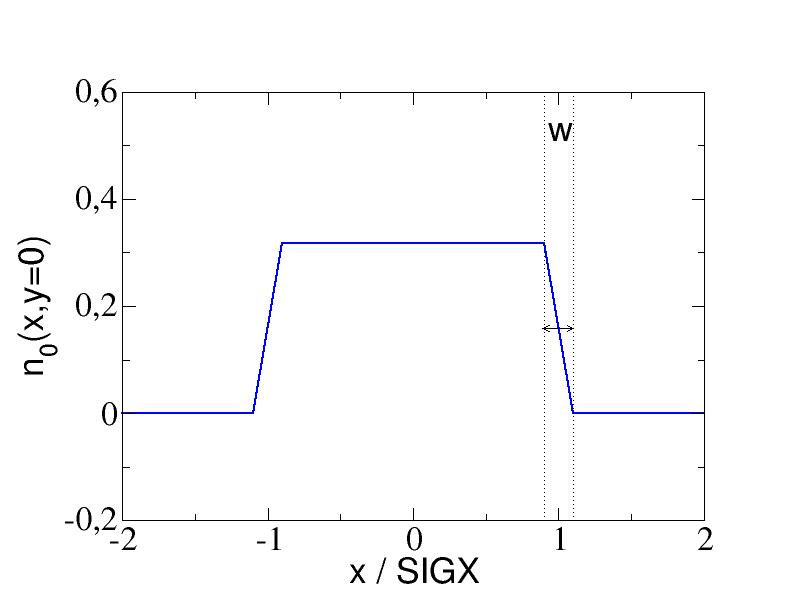
\includegraphics[width=400bp]{jpg/beambeam_n_trapez.jpg}
  \caption{Trapezoidal shape of radial density for beam-beam lens.}
  \label{fig:beambeam-n-trapez}
\end{figure}

       \item  \texttt{BBSHAPE=3}: hollow-parabolic shape (see
       fig.\ref{fig:beambeam-n-hollowparabol}). \texttt{SIGX, SIGY} are
       the distances from the centre to the maximum of the parabolic
       density profile in horizontal and vertical directions. \\
       Only circular opposite beam is possible, \textsl{i.e.} in the
       calculations \texttt{SIGX' = SIGY' = (SIGX+SIGY)/2} is
       used, if \texttt{SIGX} and \texttt{SIGY} have different
       values. \\
       \texttt{WIDTH} denotes the full width at half
       maximum of the parabolic density profile in units of
       \texttt{SIGX}, or \texttt{SIGX'} and \texttt{SIGY'},
       respectively, if \texttt{SIGX} and \texttt{SIGY} are
       not equal. Condition: \texttt{WIDTH \textless SQRT(2.0)}

\begin{figure}[h]
  \centering
  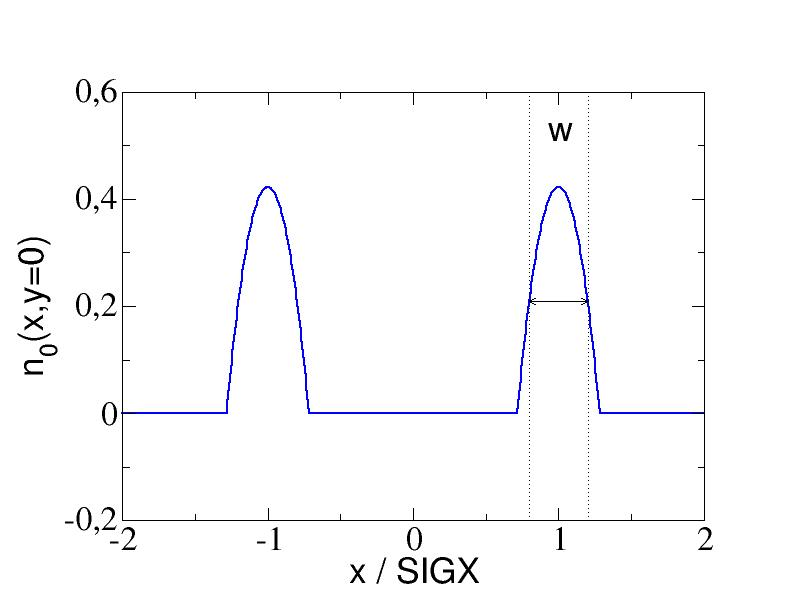
\includegraphics[width=420bp]{jpg/beambeam_n_hollowparabol.jpg}
  \caption{Hollow parabolic shape of radial density for beam-beam lens.}
  \label{fig:beambeam-n-hollowparabol}
\end{figure}

     \end{itemize}

     The restriction to circular opposite beams in the cases \texttt{BBSHAPE=2,3}
     appears to be sufficient, because such beam profiles are more important
     for the description of the interaction between the particle beam and
     an electron beam of an electron cooler, which are usually circular.


   \ttitem{BBDIR} A parameter to select the direction of motion of the
     opposite beam relative to the beam being studied. It determines
     the sign of the Lorentz force between both beams (default: -1):
     \begin{itemize}
        \item  \texttt{BBDIR=-1}: Beams move in opposite directions as in a
        collider. The Lorentz force enhances the beam-beam interaction.
        \item  \texttt{BBDIR=0}: Opposite beam does not move. The Lorentz force is
        neglected
        \item  \texttt{BBDIR=1}: Beams move in the same direction as in an
        electron cooler. The Lorentz force reduces the beam-beam interaction.
     \end{itemize}
     Note:
     \begin{itemize}
        \item  The particles in the beam considered may have a momentum
        deviation given by \texttt{DELTAP} defined in the
        \hyperref[sec:track]{\texttt{TRACK}} command.
        \item  The opposite beam is assumed to have the velocity according to
        the unperturbed energy of the particles in the beam considered. Only
        the direction of motion can be chosen.
        \item  In the case of motion in the opposite direction
        (\texttt{BBDIR=-1}), the time of interaction between the beams
        is given by \texttt{tau=length/(2*beta*clight)}, where
        \texttt{length} is the length of a bunch in the opposite beam.
        In the case of motion in the same direction (\texttt{BBDIR=1})
        as in an electron cooler, this time is given by
        \texttt{tau=length/(beta*c\_light)}, where \texttt{length} is
        the length of the cooler. Note that the factor 1/2 is inserted
        only for \texttt{BBDIR=-1} to calculate correct results.
     \end{itemize}

\end{madlist}


A beam-beam element requires the particle
\hyperref[sec:beam]{\texttt{ENERGY}} and the particle
\hyperref[sec:beam]{\texttt{CHARGE}}, as well as the number of particles
per bunch (\hyperref[sec:beam]{\texttt{NPART}}) to be set by a
\hyperref[sec:beam]{\texttt{BEAM}} command before any
calculation is performed.

Example of a four-dimensional beam-beam element definition in Collider
regime:
\madxmp{
beam,   particle = positron, npart = 1.e12, energy = 50.0; \\
bb:     beambeam, sigx = 1.e-3, sigy = 5.e-4, charge = 1.;
}

\section{Wire}
\label{sec:wire}
\madbox{
label: WIRE, \= CURRENT=\{real, \ldots \}, L=real,  \\
               \> L\_INT=\{real, \ldots \}, L\_PHY=\{real, \ldots \}, \\
               \> XMA=\{real, \ldots \}, ..., YMA=\{real, \ldots \};
}

The \texttt{WIRE} element allows defining one or several WIRE elements at once. 
\begin{madlist}
   \ttitem{L} The length of the element in the sequence.
   \ttitem{CURRENT} The current for the wires in Amperes . 
   \ttitem{L\_PHY} This should correspond to the actual physical length of the wires. 
   \ttitem{L\_INT} The length where we stop integrating the effect of the field.
   It needs to be larger or the same as \texttt{L\_PHY}.
   \ttitem{XMA} This specifies the horizontal offset of the wire compared to the reference orbit. 
   \ttitem{YMA} This specifies the vertical offset of the wire compared to the reference orbit. 
\end{madlist}

The WIRE as implemented in MAD-X is imlemented as a thin kick. However, it is still 
possible to define a length of the wire but internally the element is 
placed in the middle and drift spaces are placed on each side of the \texttt{WIRE}.
Note also that the collimator element has the same attiributes as the \texttt{WIRE}
and by defining it using the same parameters you can also get the collimator with a wire
inside. 



%  Changed by: Frank Schmidt, 25-June-2003
\section{Arbitrary Matrix Element}

\madbox{
label: MATRIX, \= TYPE=string, L=real,  \\
               \> KICK1=real,..., KICK6=real, \\
               \> RM11=real, ..., RM66=real, \\
               \> TM111=real, ..., TM666=real;
}

The \texttt{MATRIX} element allows the definition of an arbitrary transfer matrix.
It has four real array attributes:
\begin{madlist}
   \ttitem{L} Length of the element, which may be zero.
   \ttitem{KICKi} Defines the kick of the element acting on the six phase
     space coordinates.
   \ttitem{RMik} Defines the linear transfer matrix ($6\times6$ terms) of the element.
   \ttitem{TMikl} Defines the second-order terms ($6\times6\times6$ terms) of the element.
\end{madlist}

Data values that are not explicitly entered are taken from the identity
transformation for the \texttt{RMik} matrix elements, and taken as zero
for the \texttt{KICKi} kick factors and the \texttt{TMikl} second order
terms.
In the \hyperref[chap:thintrack]{thin-lens tracking
module} a non-zero length for an arbitrary matrix is accepted, however
no non-zero second order terms are allowed to avoid non symplectic
tracking runs. In the latter case the tracking run is aborted.


%\section{Coordinate Transformations}
\section{Rotation around the vertical axis}
\label{sec:yrotation}

The element \texttt{YROTATION} rotates the
\hyperref[subsec:local-straight]{straight reference system} about the
vertical (\textit{y}) axis.

\madbox{
label: YROTATION, ANGLE=real;
}

\texttt{YROTATION} has no effect on the beam, but it
causes the beam to be referred to the new coordinate system  \\
\begin{equation}\begin{split}
x_2 &= x_1 \cos\theta - s_1 \sin\theta \\
s_2 &= x_1 \sin\theta + s_1 \cos\theta
\end{split}\end{equation}
%%\textit{x}$_2$=\textit{x}$_1$cos(theta)-\textit{s}$_1$sin(theta), \\
%%\textit{y}$_2$=\textit{x}$_1$sin(theta)+\textit{s}$_1$cos(theta).\\

It has one real attribute:
\begin{madlist}
   \ttitem{ANGLE} The rotation angle $\theta$ (default: 0 rad).
\end{madlist}

A positive angle means that the new reference system is rotated
clockwise about the local \textit{y}-axis with respect to the old system.

\textbf{Important note:} \\
The rotation angle $\theta$ must be \emph{small}, \textsl{i.e.} it must be at
most comparable to the transverse angles of the orbit.

Example:
\madxmp{
KINK: YROTATION, ANGLE = 0.0001;
}

\section{Rotation around the horizontal axis}
\label{sec:xrotation}

The element \texttt{XROTATION} rotates the
\hyperref[subsec:local-straight]{straight reference system} about the
vertical (\textit{x}) axis.

\madbox{
	label: XROTATION, ANGLE=real;
}

\texttt{XROTATION} has no effect on the beam, but it
causes the beam to be referred to the new coordinate system  \\
\begin{equation}\begin{split}
y_2 &= y_1 \cos\theta - s_1 \sin\theta \\
s_2 &= y_1 \sin\theta + s_1 \cos\theta
\end{split}\end{equation}
%%\textit{x}$_2$=\textit{x}$_1$cos(theta)-\textit{s}$_1$sin(theta), \\
%%\textit{y}$_2$=\textit{x}$_1$sin(theta)+\textit{s}$_1$cos(theta).\\

It has one real attribute:
\begin{madlist}
	\ttitem{ANGLE} The rotation angle $\theta$ (default: 0 rad).
\end{madlist}

A positive angle means that the new reference system is rotated
clockwise about the local \textit{x}-axis with respect to the old system.

\textbf{Important note:} \\
The rotation angle $\theta$ must be \emph{small}, \textsl{i.e.} it must be at
most comparable to the transverse angles of the orbit.

Example:
\madxmp{
	KINK: XROTATION, ANGLE = 0.0001;
}

\section{Rotation around the longitudinal axis}
\label{sec:srotation}

The element \texttt{SROTATION} rotates the
\hyperref[subsec:local-straight]{straight reference system} about the
longitudinal (\textit{s}) axis.

\madbox{
label: SROTATION, ANGLE=real;
}

\texttt{SROTATION} has no effect on the beam, but it causes the beam to be
referred to the new coordinate system \\
\begin{equation}\begin{split}
x_2 &= x_1 \cos\psi - y_1 \sin\psi \\
y_2 &= x_1 \sin\psi + y_1 \cos\psi
\end{split}\end{equation}

%%\textit{x}$_2$=\textit{x}$_1$cos(psi)-\textit{y}$_1$sin(psi),\\
%%\textit{y}$_2$=\textit{x}$_1$sin(psi)+\textit{y}$_1$cos(psi).\\

It has one real attribute:
\begin{madlist}
   \ttitem{ANGLE} The rotation angle $\psi$ (default: 0 rad)
\end{madlist}

A positive angle means that the new reference system is rotated
clockwise about the \textit{s}-axis with respect to the old system.

Example:
\madxmp{
ROLL1: SROTATION, ANGLE=  PI/2.; \\
ROLL2: SROTATION, ANGLE= -PI/2.; \\
HBEND: SBEND, L=6.0, ANGLE=0.01; \\
VBEND: LINE=(ROLL1,HBEND,ROLL2); \\
}
The \texttt{VBEND} definition above is a way to represent a bend down in the
vertical plane, it could be defined more simply by
\madxmp{
VBEND: SBEND, L=6.0, K0S=0.01/6;
}

\section{Coordinate translation}
\label{sec:translation}

The element \texttt{TRANSLATION} changes the
\hyperref[subsec:local-straight]{reference system}
by applying a translation of the reference system.

\madbox{
label: TRANSLATION, \= DX=real,  \= DY=real,  \= DS=real;
}

\texttt{TRANSLATION} moves the coordinate system. \texttt{DX} and \texttt{DY} will translate the position and \texttt{DS} will introduce a virtual drift.

\section{Change of reference system}
\label{sec:changeref}

The element \texttt{CHANGEREF} changes the
\hyperref[subsec:local-straight]{reference system}
by applying both translations and rotations.

\madbox{
label: CHANGEREF, \= PATCH\_ANG={real, real, real}, \\
                  \> PATCH\_TRANS={real, real, real};
}

\texttt{CHANGEREF} has no effect on the beam, but it causes the beam to
be referred to the new coordinate system where both translations and
rotations are applied.

\section{SixTrack Marker}

\madbox{
label: SIXMARKER, \= ELTYPE=real, ATTR=\{real, \ldots \},  \\
               \> F3STRING=string, F3VECTOR=\{real, \ldots \} ;
}
The \texttt{SIXMARKER} element allows the definition of a marker that is converted to SixTrack.
The element has no effect in MAD-X.
\begin{madlist}
   \ttitem{ELTYPE} is the element type number in SixTrack, converted to the first column in fc.2.
   \ttitem{ATTR} This defines the remaining columns of the fc.2 file.
   \ttitem{F3STRING} Defines the String that is written to the fc.3 file, \{newline\} creates a new line in the output
   and \{0\}\ldots\{10\} are being replaced with the values in \texttt{F3VECTOR}.
   \ttitem{F3VECTOR} The values defined will be converted to the location defined in the \texttt{F3STRING}. 
\end{madlist}
\textbf{Example:}
\madxmp{
sm1:SIXMARKER, ELTYPE=2, ATTR=\{0.1,2,3,4,5,6,7\}, \\
,F3STRING="NEW\_ELEMENT \{newline\} \{0\}, \{1\} \{newline\} NEXT",\\
F3VECTOR=\{0.2, 0.5\};\\
}
Will produce in the output file fc.3:
\madxmp{
NEW\_ELEMENT \\                                                                                                  
2.00000000e-01, 5.00000000e-01 \\                                                                                         
NEXT
}

%%% END
      % Physical Elements and Markers
\include{ranges}        % Ranges and Classes
\include{line}          % Beamlines
\include{sequence}      % Sequences

\part{Input and Output}
\include{tfs}           % TFS format
%%%\title{SIXTRACK Convertor}
%  Changed by: Mark HAYES, 19-Sep-2002 


\chapter{Conversion to \textit{SixTrack}}
\label{chap:sixtrack}

\textit{SixTrack}\cite{SixTrack}\cite{SixTrack-www} is a separate beam 
optics code that is often used for long term tracking of particles, 
\textsl{e.g.} for dynamic aperture studies, because of its speed and
controllability.  

However the input files are notoriously difficult to produce by
hand. This command may be used to generate \textit{SixTrack} input files
from a sequence loaded in \madx. 


\madbox{
  SIXTRACK, \=CAVALL=logical, \\
            \>MULT\_AUTO\_OFF=logical, MAX\_MULT\_ORD=integer, \\
            \>SPLIT=logical, APERTURE=logical, RADIUS=real, MARKALL=logical;
}
 
The parameters are defined as: 
\begin{madlist}
   \ttitem{CAVALL} (optional flag) This puts a cavity element
   (\textit{SixTrack} identifier 12) with Volt, Harmonic Number and Lag
   attributes at each location in the machine. Since for large hadron
   machines the cavities are typically all located at one particular
   spot in the machine and since many cavities slow down the tracking
   simulations considerably all cavities are lumped into one and located
   at the first appearance of a cavity. This default is enforced by
   omitting this flag.  

   \ttitem{MULT\_AUTO\_OFF} (optional flag, default = FALSE) If
   TRUE, this module does not process zero value multipoles. 
   Moreover, multipoles are prepared by \texttt{SIXTRACK}
   (output file fc.3) to be treated up to the order as specified with
   \texttt{MAX\_MULT\_ORD}.  

   \ttitem {MAX\_MULT\_ORD} (optional parameter, default = 11) Process up
   to this order for \texttt{MULT\_AUTO\_OFF = TRUE}.  

   \ttitem{SPLIT} (optional flag) OBSOLETE. This splits all the
   elements in  two. This is for backward compatibilty only. The user
   should now use the \hyperref[chap:makethin]{\texttt{MAKETHIN}} command
   instead.   

   \ttitem{APERTURE} (optional flag) flag to convert the apertures
   from \madx to \textit{SixTrack} so that \textit{SixTrack} can track
   with apertures defined. The aperture data is found in file
   \texttt{fc.3.aper}. 

   \ttitem{RADIUS} (optional, default value is 1~m). This sets the
   reference  radius for the magnets. This argument is optional but
   should normally be set. 

   \ttitem{MARKALL} (optional flag, default false) flag to convert all markers through the conversion. If false, only markers with names beginning with "ip" or "mt\_" are kept.

   \ttitem{LONG\_NAMES} (optional flag, default true) flag to increase the possible length of names (from 17 to 48) and increase the number of digits in the output in the conversion. 

   \ttitem{SIX\_VERSION} (optional, default value=0) Some new formats are only supported in recent versions of SixTrack. In order to output in these formats a version number higher or equal to the number when it was implemented needs to be set. If the needed SixTrack version is 5.02.03 then the version should be set to 50203.

\end{madlist}

\textbf{Important Notes:}
\begin{itemize} 
\item The files contain all information concerning optics, field errors
 and misalignments. Hence these should all be set and a   
\madxmp{TWISS, SAVE;}
command should always be issued before calling the \texttt{SIXTRACK} command.

\item The \hyperref[sec:bvflag]{BV flag} is presently ignored by \texttt{SIXTRACK}.

%% 2015-Oct-08  19:26:14  ghislain: change this after name mangling introduced
\item \textit{SixTrack} and the \madx command \texttt{SIXTRACK} are
  presently set up for names of a maximum of 16 characters!!!!! 
  Therefore, it is mandatory to respect this limit for \madx names.
\end{itemize}

The \texttt{SIXTRACK} command always produces at least one output file: 
\begin{itemize}
   \item  fc.2 -  the basic structure of the lattice. 
\end{itemize} 
It may also produce any or all of the following files, depending on the
sequence and command attributes:
\begin{itemize}
   \item  fc.3 -   multipole mask(s). 
   \item  fc.3.aux -  various beam parameters. 
   \item  fc.3.aper - aperture element data (units are \texttt{mm} and \texttt{degrees}).
   \item  fc.8 -   misalignments and tilts. 
   \item  fc.16 -  field errors and/or combined multipole kicks. 
   \item  fc.34 -  various optics parameters at various
     locations \\ This file is not needed by \textit{SixTrack} but may
     be used as input to the program \textit{SODD}\cite{SODD}.)   
\end{itemize}  

For a full description of these files see the \textit{SixTrack} 
website\cite{SixTrack-www}, the \textit{SixTrack} user 
manual\cite{SixTrack}; and for information on running {\textit SixTrack} 
see the \textit{SixTrack} run environment description\cite{SixTrack-RE}.

%% EOF
           % Conversion to Sixtrack Input Format
\include{sxf}           % SXF file input and output
\include{plot}
%%\title{RLOT}

\section{RPLOT}

RPLOT is a MAD-X plug-in that privides additional functionality using
\href{http://root.cern.ch}{ ROOT }.  It contains several tools   

\begin{description}

\item[\textbf{ RVIEWER }] 
\textit{ plotting tool that handles the results in paramremtric form }

What makes it different      from the standard PLOT module of MAD-X is
that it is also able to      deal with the parmateric results. RPLOT
proviedes graphical user interface      that allows to choose which
functions shall be drawn, set its ranges     and adjust all the details
of the plot formatting. Of course, the result     is immendiately
visible on the screen, in contrary to the standard plot tool     that is
able to work solely in the batch mode. The user can choose several
formats to save his plot, including postscript, gif, pdf, root macro and
many      others.       

RVIEWER is able to draw the lattice functions     
\begin{enumerate}
   \item  along the layout 
   \item  at given position in function of one or two knobs  
\end{enumerate}     

It provides a convienient way to set the knob values. As the value is
set,      the plotted functions are immediately drawn for the new value.            

In order to run RVIEWER simpy issue "rviewer;" command        

\item[\textbf{ RTRACKSTORE }] 
\textit{ enables storage of the tracking data in ROOT NTuple/Tree format }

Ntuple and its modern extension called Tree are formats designed
for storing particle tracking data. It is proven to provide       the
fastest data writing and reading thanks to column wise       I/O
operations. It is commonly used for data storage by HEP
experiments. Additionally, ROOT provides automatical        ZIP data
compression that is transparent for the user algorithms.
Morover, ROOT provides wide set of very comfortable tools       for
advanced analysis and plotting of the data stored in Trees.    

Addtionally, we plan to extend RVIEWER functionality that would provide
intuitive graphical user interface to most commonly used       features
in particle tracking in accelerators. Thanks to that,       the user is
not forced to learn how to use the ROOT package.    

Currently the feature is enabled only for tracking using        the
ptc\_trackline command, however, it will be extended to       other
tracking modes.           
\end{description}

\textbf{ Download } \\
The newest version is available \href{download/}{ here }\\

\textbf{ Installation }\\
Prerequisite: ROOT must be installed beforehand compilation and whenever
the user wants to use the plug-in. See explanations on
\href{http://root.cern.ch}{ROOT webpage}.  \\ 

To install RPLOT 
\begin{enumerate}
   \item  Unpack the archive, it will create directory rplot    
\begin{verbatim}
   tar xvzf rplot-X.XX.tgz
\end{verbatim}

   \item Change to rplot directory    
\begin{verbatim}
   cd rplot
\end{verbatim}

   \item Type     
\begin{verbatim}
   make install
\end{verbatim}
\end{enumerate}

\textbf{ Examples}


\textbf{SYNOPSIS}
\begin{verbatim}
RVIEWER; 
\end{verbatim}


\textbf{ PROGRAMMERS MANUAL  } \\

 To be continued... 

         % probably material for an appendix
\include{rplot_index}   % ditto

\part{\mad Modules}
1-7     *     skip         # head
*       *     any abs=1e-20 rel=1e-10
        % SURVEY: geometric layout and survey
%%\title{Twiss Module}
%  Changed by: Chris ISELIN, 27-Jan-1997 
%  Changed by: Frank Schmidt, 11-Jul-2002 
%  Changed by: Hans Grote, 15-Jan-2003 
%  Changed by: Frank Schmidt, 06-APR-2003 
%  Changed by: ghislain 18-JUN-2014   

%  Last changed: Irina Tecker, 12-OCT-2016 

\chapter{Twiss Module}
\label{chap:twiss}

The \texttt{TWISS} command calculates the
\hyperref[subsec:tables-linear]{linear lattice
  functions} \cite{Courant-Snyder1958}, and optionally the
\hyperref[subsec:tables-chrom]{chromatic functions}. 
The coupled functions are calculated in the sense of
Edwards and Teng\cite{edwards1973}.
For the uncoupled cases they reduce to the C and S functions. 

\madbox{
TWISS, \=SEQUENCE=seqname, LINE=linename, RANGE=range,\\
       \>DELTAP=real\{,real\}||initial:final:step,\\
       \>CHROM=logical, RMATRIX=logical, TAPERING=logical,\\
       \>CENTRE=logical, TOLERANCE=real,\\
       \>FILE=filename, TABLE=tabname, NOTABLE=logical,\\
       \>SECTORMAP=logical, SECTORTABLE=tabname,\\
       \>SECTORFILE=filename, SECTORPURE=logical,\\
       \>EIGENVECTOR=tabname, EIGENFILE=filename,\\
       \>KEEPORBIT=name, USEORBIT=name,\\
       \>COUPLE=logical, EXACT=logical, \\
       \>RIPKEN=logical, TAPERING=logical \\;
}

The  attributes of the \texttt{TWISS} command are: 
\begin{madlist}
  \ttitem{SEQUENCE} the name of a valid sequence for
  which the calculation of optical functions should be performed. \\ 
  \texttt{SEQUENCE} and \texttt{LINE} are mutually exclusive.\\
  (Default: sequence or beam line defined in the latest \texttt{USE}
  command) 

  \ttitem{LINE} the name of a valid beamline for which
  the calculation of optical functions should be performed. \\
  \texttt{SEQUENCE} and \texttt{LINE} are mutually exclusive.\\
  (Default: sequence or beam line defined in the latest \texttt{USE}
  command) 
  
  \ttitem{RANGE} (Default: \texttt{\#S/\#E})\\
  The \texttt{TWISS} calculation is restricted to the specified range.
  See \hyperref[sec:range]{\texttt{RANGE}}.  

  \ttitem{DELTAP}=\texttt{real\{,real\}} or \texttt{initial:final:step}
  (Default: 0.0)\\ 
  The relative energy error \texttt{DELTAP} may be entered in one of the
  two forms above. \\ 
  The first form lists several numbers, which may be general expressions,
  separated by commas. The second form specifies an initial value, a final
  value, and a step, which must be constant expressions, separated by
  colons. \\
  For example, \texttt{DELTAP=0.001} defines a single value, 
  \texttt{DELTAP=0.001,0.005} defines two values and 
  \texttt{DELTAP=0.001:0.007:0.002} defines four values. 


  \ttitem{CHROM} a logical flag to trigger computation of the
  \hyperref[subsec:tables-chrom]{chromatic functions} as well as the radiation 
  synchrotron integrals. \\
   %irina
  \textit{Please note that the calculation is done without taking coupling into 
  account. In case of coupled lattice the warning isissued that the calculation 
  of chromatic functions can be inaccurate!}\\
  \textit{Please note that this option also changes the way that the
    chromaticities are calculated: The chromaticities are normally
    calculated from the analysis of the first and second order
    matrices. With \texttt{CHROM}, the chromaticities are recalculated by
    explicitely calculating the tunes for the case of the specified momentum
    deviation \texttt{DELTAP} and for the case of a momentum deviation equal
    to \texttt{DELTAP}+1.e-6. The tune differences divided by 1.e-6 yield the
    chromaticities.}

  \ttitem{CENTRE} a logical flag to enforce the calculation of the
  \hyperref[subsec:tables-linear]{linear lattice functions} at the
  center of the element instead of the end of the element. The values in
  the tables and in the output files are affected by this
  flag. \\ (Default: false) \\ 
  \textit{ Since the lattice functions are calculated inside the element
    the closed orbit coordinates in the output also include the misalignment
    of the element.}  

  \ttitem{TOLERANCE} the maximum closed orbit error, for all six orbit 
  components, that can be tolerated during the closed orbit search. 
  The value given in the \texttt{TWISS} command is only valid for the current 
  calculation; 
  the \hyperref[sec:coguess]{\texttt{COGUESS}} command allows to 
  change the default value for all subsequent closed orbit search calculations. 
  \\ (Default: 1.e-6)

  \ttitem{FILE} causes \madx to write a \hyperref[chap:tfs]{TFS Twiss table} 
  to the file specified. (Default: ``twiss'') \\
  The columns of the table can be selected using the \texttt{SELECT}
  command with the \texttt{FLAG=twiss} attribute. 

  \ttitem{TABLE} the name of the table where 
  \hyperref[subsec:tables-linear]{linear lattice functions} as well 
  as \hyperref[subsec:tables-chrom]{chromatic functions} are stored. 
  (Default: ``twiss'') \\
%  \madx creates a full
%  \hyperref[subsec:tables-linear]{Twiss table} in
%  memory and gives it the name \texttt{TWISS}, unless \texttt{TABLE=tabname}
%  is given, then it is called "tabname". This table
%  includes linear lattice functions as well as the chromatic
%  functions for all positions.\\
  \textbf{Note:} If the \texttt{TABLE} option is given the selection of column 
  names via the \texttt{SELECT} command is ignored. Hence if both \texttt{TABLE} and
  \texttt{FILE} options are given, the table written to file is the full
  twiss table, containing all elements as rows and all known Twiss 
  parameters as columns. 

  \ttitem{NOTABLE} logical flag to prevent the creation of the internal twiss
  table. Consequently, no output file is created either.  \\ 
  (Default: false)
  

  \ttitem{RMATRIX} If this flag is used the the one-turn map at the
  location of every element is calculated and prepared for
  storage in the twiss table. Using the
  \hyperref[sec:select]{\texttt{SELECT}} command and using
  the column \texttt{RE, RE11 \ldots RE16 \ldots RE61 \ldots RE66} these
  components will be added to the twiss table, i.e. with \texttt{"COLUMN, RE"} and
  \texttt{"COLUMN, REij"} one gets all or the component "ij" respectively.    

  \ttitem{SECTORMAP} a logical flag to initiate the calculation of a 
  \hyperref[sec:sectormap]{sector map}. Default the Rij contains feed-down from higher order maps. In order to turn it off use the flag SECTORPURE. 
  
  \ttitem{SECTORACC} a logical flag to save composition of maps instead of individual maps of a
  \hyperref[sec:sectormap]{sector map}.

  \ttitem{SECTORPURE} a logical flag to save the transfer map Rij without effects from higher order map (Tijk). This option should be used to get it in the correct format for TRAIN.

  \ttitem{SECTORTABLE} the name of the table containing the \texttt{SECTORMAP}
  values. The elements (lines) and parameters (columns) 
  of the table can be tailored using the \hyperref[sec:select]{\texttt{SELECT}} 
  command as specified in \hyperref[sec:sectormap]{\texttt{SECTORMAP}} \\
  (Default: sectortable)

  \ttitem{SECTORFILE} the name of the file to which the \texttt{SECTORMAP} is
  written. 
  In order to specify the output use the SECTORTABLE as specified in
  \hyperref[sec:sectormap]{\texttt{SECTORMAP}} \\
  (Default: "sectormap")
  %% Used to write SECTORMAPs to the file
  %% SECTORFILE="filename", if missing the output of SECTORMAP
  %% will go to the file "sectormap" with the format as found in
  %% \href{../Introduction/sectormap.html}{SECTORMAP}.    

  \ttitem{EIGENVECTOR} a logical flag to output the eigenvectors in the beginning of the sequence. Multiplying with this matrix brings normalized coordinates to physical coordinates.
  \ttitem{EIGENFILE} the name of the file to which the \texttt{EIGENVECTOR} is written. 

  \ttitem{KEEPORBIT} The keeporbit attribute (with an optional name,
  keeporbit="name") stores the orbit under this name at the
  start, and at all monitors.    

  \ttitem{USEORBIT} The useorbit attribute (with an optional name,
  useorbit="name") uses the start value provided for the closed
  orbit search; the values at the monitors are used by the
  threader.    

  \ttitem{COUPLE} (obsolete) This \madeight option can no
  longer be set since TWISS in \madx is always calculated in
  coupled mode. \madx computes the coupled functions in the
  sense of Edwards and Teng \cite{edwards1973}. 
  For the uncoupled cases they reduce to the C and S functions. 

  \ttitem{EXACT} If this is used the dirft is expanded around the actual
  closed orbit instead of the ideal orbit. (Default: false)   
  
  \textit{ Twiss calculation is 4D only!} : The \texttt{TWISS}
  command calculates an approximate 6D closed orbit when the
  accelerator structure includes an active
  \hyperref[sec:rfcavity]{cavity}. However, the
  calculation of the Twiss parameters are 4D only. This may
  result in apparently non-closure of the beta values in the
  plane with non-zero dispersion. The full 6D Twiss parameters
  can be calculated with the
  \hyperref[chap:ptc-twiss]{PTC\_TWISS} command.    

  \ttitem{RIPKEN} This flag calculates the Ripken-Mais Twiss
  parameters (\texttt{beta11, beta12, beta21, beta22, alfa11, alfa12,
  alfa21, alfa22, gamma11, gamma12, gamma21} and \texttt{gamma22}) using
  the parameters \texttt{betx, bety, alfx, alfy, \\ gamax, gamay, R11, R12,
    R21} and \texttt{R22} as input.

  \ttitem{TAPERING} Adjust the strengths of the quadrupoles and sextupoles
  in order to compensate for the offset in energy. This flag triggers a
  call to the \hyperref[chap:taper]{\texttt{TAPER}} command with default
  parameters and no output file. 
  %% The phase of the RF is
  %% also adjusted in order to find a closed 6D orbit. The change of the 
  %% attributes are stored in k1tap, k2tap etc.  

\end{madlist}

The tables are suitable for \hyperref[chap:plot]{\texttt{PLOT}}.

After a successful \texttt{TWISS} run \madx creates a 
table of summary parameters named "SUMM" which includes tunes,
chromaticities, etc. versus the selected values of \texttt{DELTAP}.
Please note that with the \texttt{CHROM} attribute the calculation is done without
taking coupling into account. In case of coupled lattice the warning isissued that
the calculation of chromatic functions can be inaccurate!

Notice also that in \madx, \texttt{DELTAP} is converted to \texttt{PT},
which is used as longitudinal variable. 
Dispersive and chromatic functions are hence derivatives with
respect to \texttt{PT}. (see \hyperref[subsec:tables-summ]{summ table}). 

These summary parameters can later be accessed via the 
\hyperref[chap:tables]{table access functions} using the "SUMM" table.  

\section{Twiss Parameters for a Period}
\label{sec:twissperiod}

The simplest form of the \texttt{TWISS} command is
\madbox{
TWISS;
}
which calculates the periodic solution for the last beamline or sequence
declared in a \texttt{USE} statement, and with zero \texttt{DELTAP}.
Chromatic functions are not calculated. 
Standard tables ("TWISS" and "SUMM") are created in memory but no file
is written to disk. 

The slightly more elaborate version 
\madbox{
TWISS, DELTAP=real\{,real\}, CHROM, TABLE=tabname;
}
computes the periodic solution, including chromatic functions, for the last beam
line or sequence declared in a \texttt{USE} statement, for all values of
DELTAP entered (or for \texttt{DELTAP=0}, if none is entered). 
The tables "tabname" and "SUMM" are created in memory and no file is
written to disk. 

\textbf{Example:} 
\madxmp{
USE, period=OCT; \\
TWISS, DELTAP=0.001, CHROM;
}
computes the periodic solution for the linear lattice and
chromatic functions for the beam line OCT and for DELTAP=0.001. 

%% Apart from saving computing time, it is equivalent to the command
%% sequence  
%% \begin{verbatim}
%% RING: LINE=(4*(OCT,-OCT));
%%       USE,period=RING;
%%       TWISS,DELTAP=0.001,CHROM;
%% \end{verbatim}

\section{Initial Values from a Periodic Line}
\label{sec:twissinitial}

It is possible to track the lattice functions starting with the periodic
solution for another beam line. If this is desired the TWISS command
takes the form  
\madbox{
TWISS, \=DELTAP=real\{,real\}, LINE=beamline, \\
       \>MUX=real, MUY=real, \\
       \>TABLE=tabname;
}
No other attributes should appear in the command. For each value of
DELTAP, \madx first searches for the periodic solution for the beam line
mentioned in LINE=beamline: The result is used as an initial condition
for the lattice function tracking. 

\textbf{Example:} 
\madxmp{
xxxxxxxx\= \kill
CELL:   \>LINE=(...); \\
INSERT: \>LINE=(...); \\
USE, period=INSERT; \\
TWISS, LINE=CELL, DELTAP=0.0:0.003:0.001, CHROM, FILE;
}

For four values of DELTAP the following happens: First \madx finds the
periodic solution for the beam line CELL: Then it uses this solution as
initial conditions for tracking the lattice functions of the beamline
CELL: Output is also written on the file TWISS:  

If any of the beam lines was defined with formal arguments, actual
arguments must be provided:  
\madxmp{
CELL(SF,SD): \=LINE=(...); \\
INSERT(X):   \>LINE=(...); \\
USE, period=INSERT; \\
TWISS, LINE=CELL(SF1,SD1);
}

\section{Given Initial Values}

Initial values for \hyperref[subsec:tables-linear]{linear
lattice functions} and \hyperref[subsec:tables-chrom]{chromatic
  functions} may also be numerical.
Initial values can be specified on the \texttt{TWISS} command:  
\madbox{
TWISS,   \=BETX=real, ALFX=real, MUX=real,\\
         \>BETY=real, ALFY=real, MUY=real,\\
         \>DX=real, DPX=real, DY=real, DPY=real,\\
         \>X=real, PX=real, Y=real, PY=real,\\
         \>T=real, PT=real,\\
         \>WX=real, PHIX=real, DMUX=real,\\
         \>WY=real, PHIY=real, DMUY=real,\\
         \>DDX=real, DDY=real, DDPX=real, DDPY=real,\\
         \>R11=real, R12=real, R21=real, R22=real,  !coupling matrix\\
         \>TABLE=tabname,\\
         \>TOLERANCE=real,\\
         \>DELTAP=real:real:real;
}

All initial values for
\hyperref[subsec:tables-linear]{linear lattice functions} and
\hyperref[subsec:tables-chrom]{chromatic functions} are
permitted, but \texttt{BETX} and \texttt{BETY} are required.
Moreover, a \hyperref[sec:beta0]{BETA0} block can be added as filled by the
\hyperref[sec:savebeta]{\texttt{SAVEBETA}} command (see below).
The lattice parameters are taken from this block, but are also
overwritten by lattice parameters explicitly decalred on the command 
line. As entered, the initial conditions cannot depend on
\texttt{DELTAP},
and can thus be correct only for one such value.  

\section{SAVEBETA}
\label{sec:savebeta}
Initial lattice parameters can be saved and transfered for later commands, in
particular for \hyperref[chap:twiss]{\texttt{TWISS}} or the
\hyperref[chap:match]{match module}, with the \texttt{SAVEBETA} command
sequence.   

\madbox{
SAVEBETA, LABEL=string, PLACE=string, SEQUENCE=sequencename;
}
marks a location given by attribute \texttt{PLACE} in an expanded
sequence \texttt{sequence\_name}; at the next \texttt{TWISS} command
execution, a \hyperref[sec:beta0]{\texttt{BETA0}} block is saved at that
location with the label given by the attribute \texttt{LABEL}. This is
done only once; in order to get a new \texttt{BETA0} block at the same
location in a subsequent \texttt{TWISS} command, the \texttt{SAVEBETA}
command  must be repeated. The content of the \texttt{BETA0} block can
then be used in other commands, \textsl{e.g.} \texttt{TWISS} and
\texttt{MATCH}. 

\textbf{Example} (after sequence expansion): 
\madxmp{
SAVEBETA, LABEL=sb1, PLACE=mb[5], SEQUENCE=fivecell; \\
TWISS; \\
SHOW, sb1;
}
saves and then shows the \texttt{BETA0} block parameters at the end (!) of the
fifth element of type \texttt{mb} in the sequence.  


Parameters in tables can also be accessed 
using the \hyperref[chap:tables]{table access} functions. 
\begin{verbatim}
USE, period=...;
SAVEBETA, LABEL=name, PLACE=place, SEQUENCE=s_name;
TWISS,...;
\end{verbatim}

When reaching the \texttt{PLACE} in the
sequence \texttt{s\_name} during execution of
\hyperref[chap:twiss]{\texttt{TWISS}}, \madx saves a
\hyperref[sec:beta0]{BETA0} block with the \texttt{LABEL} name: This
block is filled with the values of all lattice parameters in place.   

\textbf{Example 1:} 
\begin{verbatim}
USE, period=CELL;
SAVEBETA, LABEL=END, PLACE=#E, SEQUENCE=CELL;
TWISS;
USE, period=INSERT;
TWISS, BETA0=END;
\end{verbatim}
This first example calculates the \hyperref[sec:twissperiod]{periodic
  solution} of the line \texttt{CELL}, and then tracks lattice parameters through
\texttt{INSERT}, using all end conditions (including orbit) in
\texttt{CELL} at the start of \texttt{INSERT}.  

\textbf{Example 2:} 
\begin{verbatim}
USE, period=CELL;
SAVEBETA, LABEL=END, PLACE=#E, SEQUENCE=CELL;
TWISS;
USE, period=INSERT;
TWISS, BETX=END->BETY, BETY=END->BETX;
\end{verbatim}
This is similar to the first example,but the beta functions are interchanged (overwritten).  

\section{BETA0: Set Initial Lattice Parameters}
\label{sec:beta0}
Initial lattice parameters can be set 'manually' for later commands, in
particular for \hyperref[chap:twiss]{\texttt{TWISS}} or the 
\hyperref[chap:match]{\texttt{MATCH}} module, by
using the \texttt{BETA0} command attached to a label.  

\madbox{
label: BETA0, \=BETX=real, ALFX=real, MUX=real,\\
              \>BETY=real, ALFY=real, MUY=real,\\
              \>\{etc for linear and chromatic lattice functions\};
}

A \texttt{BETA0} block can be used as a whole with all values declared,
as a block with overriden values explicitly, or by extracting single
values as shown in the three examples below:

Example of \texttt{BETA0} block used as a whole in \texttt{TWISS}: 
\madxmp{
initial: BETA0, \=BETX=10., ALFX=0.0, MUX=0.0, \\
                \>BETY=10., ALFY=0.0, MUY=0.0, \\
                \>DX=1., DPX=0.0;\\
TWISS, BETA0=initial;}

Example of \texttt{BETA0} block used as a whole but with overriden
values in the \texttt{TWISS} command:
\madxmp{
initial: BETA0, \=BETX=10., ALFX=0.0, MUX=0.0, \\
                \>BETY=10., ALFY=0.0, MUY=0.0, \\
                \>DX=1., DPX=0.0;\\
TWISS, BETA0=initial, ALFX=-0.1, ALFY=0.1;}

Example of using \texttt{BETA0} block by extracting single values in the
\texttt{TWISS} command:
\madxmp{
initial: BETA0, \=BETX=10., ALFX=0.0, MUX=0.0, \\
                \>BETY=10., ALFY=0.0, MUY=0.0, \\
                \>DX=1., DPX=0.0;\\
TWISS, BETX=initial-$>$BETX, BETY=initial-$>$BETY;}


%\input{Introduction/sectormap}
\section{Sectormap output}
\label{sec:sectormap}
% Begin New version: Jean-Luc Nougaret, 18-Dec-2008 

The flag \texttt{SECTORMAP} of the \texttt{TWISS} command causes a file "sectormap" to be
written.

For each user-selected element, it contains the user-selected coefficients of 
the kick vector \texttt{K} ($6$ values), of the first-order map \texttt{R} 
($6\times6$ values) and of the second-order map \texttt{T} ($6\times6\times6$ 
values)
If only certain elemenents and values are desired a SELECT command can be used. 
Note that it should be used on the TABLE as shown in the following example:
  

\madxmp{
TWISS,,SECTORMAP,SECTORTABLE=my\_sect\_table;
SELECT, FLAG=my\_sect\_table, COLUMN=name, pos, k1, r11, r66, t111;
WRITE, TABLE=my\_sect\_table, FILE="sectormap.tfs";
}

The sectormap file contains for each selected element, one element per
line, the set of chosen K, R, and T matrix coefficients: 
\\
\\
{\footnotesize
\begin{tabular}{l|l|l}
@ NAME &              \%13s &  "MY\_SECT\_TABLE" \\ 
@ TYPE &              \%09s &  "SECTORMAP" \\ 
@ TITLE &             \%08s &  "no-title" \\ 
@ ORIGIN &           \%19s &  "MAD-X 3.04.62 Linux" \\ 
@ DATE &              \%08s &  "18/12/08" \\ 
@ TIME &              \%08s &  "10.33.58"
\end{tabular}
\\
\\
\begin{tabular}{l | l | l | l | l | l }
* NAME & POS & K1 & R11 & R66 & T111 \\ 
\$ \%s & \%le & \%le & \%le  & \%le & \%le \\ 
 "FIVECELL\$START"  & 0 & 0 & 1 & 1 & 0 \\ 
 "SEQSTART"  & 0 &  0  &  1 &  1  &  0 \\ 
 "QF.1"  & 3.1 & -1.305314637e-05 & 1.042224745 & 1 & 0 \\ 
 "DRIFT\_0" & 3.265 & 7.451656548e-21 & 1 & 1 & 0 \\ 
 "MSCBH" & 4.365 & -1.686090613e-15 & 0.9999972755 & 1 & 0.006004411526 \\ 
 "CBH.1" & 4.365 & 0 & 1 & 1 & 0 \\ 
 "DRIFT\_1" & 5.519992305 & -6.675347543e-21 & 1 & 1 & 0 \\ 
 "MB" & 19.72000769 & 2.566889547e-18 & 1.000000091 & 1 & -4.135903063e-25 \\ 
 "DRIFT\_2" & 21.17999231 & -1.757758802e-20 & 1 & 1 & 0 \\ 
 "MB" & 35.38000769 & 2.822705549e-18 & 1.000000091 & 1 & -4.135903063e-25 \\ 
 "DRIFT\_2" & 36.83999231 & 2.480880093e-20 & 1 & 1 & 0 \\ 
 "MB" & 51.04000769 & 3.006954115e-18 & 1.000000091 & 1 & -4.135903063e-25 \\ 
 "DRIFT\_3" & 52.21 & -4.886652187e-20 & 1 & 1 & 0 \\ 
... & ... & ... & ... & ... & ... \\ 
... & ... & ... & ... & ... & ... \\ 
... & ... & ... & ... & ... & ...
\end{tabular}
}
\\
\\ 
Of course, the \texttt{SELECT} statement can be combined with additional
options to filter-out the list of elements, such as in the following
statement, which for instance only retains drift-type elements:  

\madxmp{
  SELECT, \=FLAG=my\_sect\_table, CLASS=drift, \\
          \>COLUMN=name, pos, k1, r11, r66, t111;
}


\texttt{K} coefficients range: 
\texttt{K1}... 
\texttt{K6}


\texttt{R} coefficients range: 
\begin{tabular}{ccc}
\texttt{R11} & ... & \texttt{R61} \\ 
\texttt{R12} & ... & \texttt{R62} \\ 
... & ... & ... \\ 
\texttt{R16} & ... & \texttt{R66}
\end{tabular}


\texttt{T} coefficients range: 
\begin{tabular}{ccc}
\texttt{T111} & ... &\texttt{T611} \\ 
\texttt{T121} & ... & \texttt{T621} \\ 
... & ... & ... \\ 
\texttt{T161} & ... & \texttt{T661} \\ 
\texttt{T112} & ... & \texttt{T612} \\ 
... & ... & ... \\ 
\texttt{T166} & ... & \texttt{T666}
\end{tabular}

 In the above notation, 
\texttt{Rij} stands for "effect on the 
\texttt{i}-th coordinate of the 
\texttt{j}-th coordinate in phase-space", whereas 
\texttt{Tijk} stands for "combined effect on the 
\texttt{i}-th coordinate of both the 
\texttt{j}-th and 
\texttt{k}-th coordinates in phase-space" along the lattice. 
% End New Version 

%  Commented by jluc, on 18 December 2008
% The flag "sectormap" on the Twiss command (together with an element
% selection via select,flag=sectormap,...) causes a file "sectormap" to
% be written. This is a fixed format file; per selected element it
% contains:
% 
% <pre>
% end_position   element_name
% kick vector (6 values)
% first order map (6 lines with 6 values each), column-wise
% second order map (36 lines with 6 columns each, column-column-wise)
% </pre>
% 
% Or more explicitly:
% 
% <pre>
% The first line is:
% K[1] ... K[6]
% 
% Then: 
% R[1,1] ... R[6,1]
% R[1,2] ... R[6,2]
% ...
% R[1,6] ... R[6,6]
% 
% 
% Then:
% T[1,1,1] ... T[6,1,1]
% T[1,2,1] ... T[6,2,1]
% ...
% T[1,6,1] ... T[6,6,1]
% T[1,1,2] ... T[6,1,2]
% ...
% T[1,6,6] ... T[6,6,6]
% </pre>
% 
   
The maps are the accumulated maps between the selected elements. They
contain both the alignment, and field errors present. Together with the
starting value of the closed orbit (which can be obtained from the
standard twiss file) this allows the user to track particles over larger
sectors, rather than element per element. Note that effects of the higher order
are included in the Rij. In order to disable this use the flag SECTORPURE. 
This flag should be activated when used to interface TRAIN.  


%\input{threader/threader}
%%\title{Threader}

\section{Beam Threader}
\label{sec:threader}

In a machine with magnetic and alignment errors it can happen that the
beam does not circulate and the closed orbit cannot be established and
measured. This can also happen in \madx and the closed orbit finder does
not converge. 

The \texttt{THREADER} simulates beam steering through such a machine
with repeated measurement of trajectory over a certain number of
monitors and correction of the trajectory with upstream correctors.   

When enabled, threading is executed whenever a trajectory or closed
orbit search is carried out by the \hyperref[chap:twiss]{TWISS}
module.   

The threader is controlled as an option. 
The following \madx command enables the threader:
\madxmp{OPTION, THREADER;}
and the threader can be disabled with
\madxmp{OPTION, -THREADER;}

During the trajectory search in \hyperref[chap:twiss]{\texttt{TWISS}}, or the first 
turn of the orbit search for a closed machine, the threader calculates at each
monitor the difference between the present trajectory reading and a
reference value.
If the difference exceeds a threshold (see below), the threader searches
backwards for the first corrector that will efficiently cancel the
difference and calculates the corresponding kick. The trajectory is then
recalculated starting again from that corrector and progressing
forward. The calculated kicks are added to already existing kicks. If
Twiss is searching for a closed orbit which involves tracking this
trajectory over many turns, the threader is only active during the first
turn.  

The reference value for the trajectory difference is zero by default but
can also be obtained from a previous orbit calculation if the current
\texttt{TWISS} command has the \texttt{USEORBIT} flag enabled and a previous
\texttt{TWISS} command had the \texttt{KEEPORBIT} flag enabled. This allows
for example to thread the beam into a machine with orbit bumps present.  

The threshold values for triggering the threader correction can be set
with the command  
\madbox{
THREADER, VECTOR=\{xmax, ymax, att\};
}
where 
\begin{madlist}
  \ttitem{xmax, ymax} threshold orbit excursions beyond which the threader
  is applied. \\ Defaults: 0.005, 0.005
  \ttitem{att} attenuation factor for the kicks applied by the threader
  \\ Default: 1.0 
\end{madlist}

The attenuation factor defines the fraction of the calculated kick that
is actually applied by the threader.  
An attenuation factor of 0.5 will apply 50\% of the calculated kicks.

\section{Closed Orbit Guess}
\label{sec:coguess}

In order to help the initial finding of the closed orbit by the
\texttt{TWISS} module, it is possible to specify an initial guess for
the coordinates of the fixed point at the start of the lattice.

\madbox{
COGUESS, \=X=real, PX=real, Y=real, PY=real, T=real, PT=real, \\
         \>TOLERANCE=real, \\
         \>CLEAR=logical;
}

The \texttt{COGUESS} command has the following attributes:
\begin{madlist}
  \ttitem{X, PX, Y, PY, T, PT} each parameter specified defines a first guess for all future closed orbit
  searches in case they are different from zero.  
  
  \ttitem{TOLERANCE} sets the required convergence precision in the closed
  orbit search. \\ (Default: 1.e-6)  
  
  \ttitem{CLEAR} a flag to reset the tolerance to its default value and to
  cancel the effect of a previous \texttt{COGUESS} in defining a first
  guess for subsequent closed orbit searches. \\ (Default:~false) 

\end{madlist}


\textbf{Example}\\
\madxmp{
COGUESS, X=1.e-3; \\
... \\
TWISS; \\
... \\
COGUESS, Y=-2.e-3; \\
... \\
TWISS; \\
... \\
COGUESS, CLEAR; \\
... \\
TWISS; \\
... \\
}
\section{Coupling}
\label{sec:coupling}

In order to calculate Twiss parameters ($\beta$, $\alpha$ and $\phi$) MAD-X uses Edwards-Teng approach.

For coupled motion the matrix transformation can be written in a form $M = VUV^{-1}$, where $M$ is a symplectic 1-turn map, $U$ is a symplectic decoupled block-diagonal matrix, $V$ is a symplectic "rotation" matrix. Initial coupling parameters are calclulated based on decoupled $U$ matrix. 
  
Given that $M_1$ is the one-turn matrix at point 1, $M_2$ is the one-turn matrix at point 2 , and we know $M_{12}$, the transfer matrix between points 1 and 2, we can express the change of the one-turn map from point 1 to point 2 by {\color{blue} $M_2 = M_{12}M_1M^{-1}_{12}$}. Then $U_2 = V_2^{-1}M_2V_2 = V_2^{-1} {\color{blue}M_{12}M_1M^{-1}_{12}} V_2 = ( V_2^{-1} M_{12} {\color{blue}V_1) U_1 (V_1^{-1}} M^{-1}_{12} V_2)$.

So,  $U_2 = W_{12} U_1 W_{12}^{-1} \textrm{, where } W_{12} \equiv V_2^{-1} M_{12}  V_1 $
Knowing $V_1$ and $M_{12}$  (transfer matrix of the element), we can calculate $V_2 W_{12} = M_{12} V_1,$ where we use $V_{2}$ for computing the coupling parameters and $W_{12}$ to propagate to the end of the element. One can find $V_2$ such that $W_{12}$ is block-diagonal or off block-diagonal. 
  
For weakly coupled lattice MAD-X always uses \textbf{block-diagonal} solution, i.e. large tune (mode1) is associated with x-plane, and smaller tune (mode2) is associated with y-plane by convention. For a highly coupled lattice, it may happen at some places in the lattice that mode1 is associated with y-plane, and mode2 with x-plane. Switching the association of mode1 and mode2 with x and y-planes as one propagates the twiss parameters through the lattice is called "modes flip" (use \textbf{off-block diagonal} solution for $W_{12}$). In case the modes flip is triggered, there is an additional stability check, either the calculation of twiss parameters can be done with modes flip or not. 

\section{Intermediate values}

The \texttt{SELECT, FLAG=interpolate} command allows to select locations for
output of intermediate values for the \texttt{TWISS} command. If interpolation
points have been selected for an element, the \texttt{TWISS} command will add
the values at these locations to the TFS table rather than at the end of the
element.

\madbox{
SELECT, \=FLAG=interpolate, SEQUENCE=string, RANGE=string, CLASS=string, \\
        \>CLEAR, \\
        \>SLICE=integer, \\
        \>STEP=real, \\
        \>AT=\{real, \ldots \};
}

\textbf{Note:} This feature may behave unexpectecly with \texttt{CENTRE}.

Selected elements can optionally be filtered based on sequence, range and
class. Every selection specifies exactly one of the following actions which
overrides previous selections for the matching elements:

\begin{madlist}
  \ttitem{CLEAR} remove interpolation positions.
  \ttitem{SLICE} slice using a fixed number of slices.
  \ttitem{STEP} slice at every \texttt{STEP} meters.
  \ttitem{AT} slice at given locations (as fraction of the node length).
\end{madlist}


%% EOF
         % TWISS
%%\title{Matching Module}
%  Changed by: Chris ISELIN, 27-Jan-1997 
%  Changed by: Oliver Bruning, 20-Jun-2002 
%  Changed by: Hans Grote, 30-Sep-2002 
 
\chapter{Matching Module}
\label{chap:match}

Before a match operation at least one sequence must be selected by means
of a \hyperref[sec:use]{\texttt{USE}} command. Matching is 
initiated by the \hyperref[sec:match]{\texttt{MATCH}} command. The matching
module can act on more than one sequence simultaneously by  specifying
more than one sequence when initiating the matching mode.  
From this command to the corresponding
\hyperref[sec:endmatch]{\texttt{ENDMATCH}} command \madx accepts the
matching commands listed below. For a mathematical description of the
minimisation procedures see \cite{MINUIT}. 

In particular one may do the following: 
\begin{itemize}
 \item Define the sequence(s) the matching module will work on 
 \item Set initial conditions for transfer line matching 
 \item Define constraints 
 \item Define the parameters to be varied 
 \item Match by different methods. 
\end{itemize}

The matching commands are described in detail below. Some other commands
can also be issued during matching.  

\begin{itemize}
\item Enter and Leave Matching Mode
  \begin{itemize}
  \item \hyperref[sec:match]{\texttt{MATCH}}: Initiate Matching Mode
  \item \hyperref[sec:endmatch]{\texttt{ENDMATCH}}: Leave Matching Mode
  \end{itemize}
\item Define Variable Parameter
  \begin{itemize}
  \item \hyperref[sec:vary]{\texttt{VARY}}: Set Parameter to Vary
  \end{itemize}
\item Define Constraint
  \begin{itemize}
  \item \hyperref[sec:constraint]{\texttt{CONSTRAINT}}: Simple Constraint 
  \item \hyperref[sec:weight]{\texttt{WEIGHT}}: Matching Weights
  \item \hyperref[sec:global]{\texttt{GLOBAL}}: Global Constraints
  \item \hyperref[sec:gweight]{\texttt{GWEIGHT}}: Weights for Global Constraints
  \end{itemize}
\item \hyperref[sec:match-methods]{Matching Methods}
  \begin{itemize}
  \item \hyperref[subsec:match-lmdif]{\texttt{LMDIF}}: Fast Gradient Minimisation
  \item \hyperref[subsec:match-migrad]{\texttt{MIGRAD}}: Gradient Minimisation
  \item \hyperref[subsec:match-simplex]{\texttt{SIMPLEX}}: Simplex Minimisation
  \item \hyperref[subsec:match-jacobian]{\texttt{JACOBIAN}}: Newton Minimisation
  \end{itemize}
\item Expression Matching with \hyperref[sec:use-macro]{\texttt{USE\_MACRO}}
\end{itemize}

%\line(1,0){300}

%\href{http://bruening.home.cern.ch/bruening/}{Oliver Br\"uning}, June, 2002; 
%\href{http://rdemaria.home.cern.ch/rdemaria/}{Riccardo de Maria}, February, 2006. 

% add other files to the end of this file


%\input{match/match_main}
%%\title{MATCH / ENDMATCH}
%  Changed by: Chris ISELIN, 27-Jan-1997 
%  Changed by: Oliver Bruning, 20-Jun-2002 
%  Changed by: Hans Grote, 30-Sep-2002 
%  Changed by: Riccardo de Maria, 9-Jan-2008 


%% Before matching at least one
%% \href{../Introduction/sequence.html}{SEQUENCE} must be selected by means
%% of a \href{../control/general.html#use}{USE} command. The matching
%% module can act on more than one sequence simultaneously by specifying
%% more than one sequence in the \texttt{MATCH} command.


\section{MATCH \ldots ENDMATCH}
\label{sec:match}\label{sec:endmatch}

The \texttt{MATCH} command is used for matching either a \hyperref[sec:cell]{periodic cell}
or an \hyperref[sec:insertion]{insertion} to another part of the machine. 

Both matching modes are initiated by the \texttt{MATCH} command using
one of several forms outlined below. 

The \texttt{ENDMATCH} command terminates the matching section and deletes
all tables related to the matching run. 
\madbox{
ENDMATCH;
}


\section{Cell Matching}
\label{sec:cell}

The matching of a periodic cell is initiated by a \texttt{MATCH} command of
the form:

\madbox{
MATCH, \=SEQUENCE='name1', 'name2', \ldots , 'name-n', \\
       \>SLOW=logical;
}

In this first mode the matching routine is initiated only with one
attribute specifying the sequence(s) the matching module will work
on. In this matching mode the periodicity of the optics functions is
enforced at the beginning and end of the selected range. 
\madxmp{MATCH, SEQUENCE='name1', 'name2', \ldots ,'name-n';}
    


\section{Insertion Matching}
\label{sec:insertion}
The matching of an insertion to another part of the machine is initiated
by a \texttt{MATCH} command taking one of the following forms:

\madbox{
MATCH, \=SEQUENCE= 'name1', 'name2', \ldots , 'name-n',\\
       \>BETA0= 'beta01', 'beta02', \ldots , 'beta0n', \\
       \>SLOW=logical;
}

or

\madbox{
MATCH, \=SEQUENCE='seqname', \\ 
       \>BETX=real, ALFX=real, MUX=real, \\
       \>BETY=real, ALFY=real, MUY=real, \\
       \>X=real, PX=real, Y=real, PY=real, \\
       \>DX=real, DY=real, DPX=real, DPY=real, \\
       \>DELTAP=real, SLOW=logical;
}

In the second mode, called insertion matching, the matching routine is
initiated with two attributes: one specifying the sequence(s) the
matching module will work on and one specifying the initial conditions
of the optic functions for each sequence. In this case the initial
values are assumed as exact. 
    
\textbf{Specification of Initial Values:}
The initial values of the optical
functions  for the insertion matching can either be specified in form of
a \hyperref[sec:savebeta]{\texttt{SAVEBETA}} command or by
explicitly stating the individual optic function values after the
\texttt{MATCH} command. The two options can be entered as         
\madxmp{
  MATCH, \=SEQUENCE= 'name1', 'name2',.., 'name-n',\\
         \>BETA0= 'beta01', 'beta02',..., 'beta0n';
}
or
\madxmp{
  MATCH, \=SEQUENCE='seqname', \\ 
         \>BETX=real, ALFX=real, MUX=real, \\
         \>BETY=real, ALFY=real, MUY=real, \\
         \>X=real, PX=real, Y=real, PY=real, \\
         \>DX=real, DY=real, DPX=real, DPY=real, \\
         \>DELTAP=real;
}

\textbf{Example 1:}   
\begin{verbatim}
CELL: SEQUENCE=(...) ;
INSERT: SEQUENCE=(...) ;
USE, PERIOD=cell;
SAVEBETA, LABEL=bini, PLACE=#e;
TWISS, SEQUENCE=cell;
USE, PERIOD=insert;
MATCH, SEQUENCE=insert, BETA0=bini;
CONSTRAINT, SEQUENCE=insert, RANGE=#e, MUX=9.345, MUY=9.876;
\end{verbatim}

This matches the sequence 'INSERT' with initial conditions to a new
phase advance. The initial conditions are given by the periodic solution
for the sequence CELL1. 
    
\textbf{Example 2:}	
\begin{verbatim}
USE, PERIOD=insert;
MATCH, SEQUENCE=insert;
CONSTRAINT, SEQUENCE=insert, RANGE=#e, MUX=9.345, MUY=9.876;
\end{verbatim}
This matches the beam line 'INSERT' with periodic boundary conditions to
a new phase advance. 

The initial conditions can also be transmitted by a combination of a
\hyperref[sec:savebeta]{\texttt{SAVEBETA}} command and explicit
optic function specifications: 
\begin{verbatim}
USE, cell1;
SAVEBETA, LABEL=bini, PLACE=#E;
TWISS, SEQUENCE=cell1;
USE, PERIOD=line1;
MATCH, SEQUENCE=line1, BETA0=bini, MUX=1.234, MUY=4.567;
\end{verbatim}

This example transmits all values of the \texttt{SAVEBETA} array 'bini' as
initial values to the \texttt{MATCH} command and overrides the initial phase
values by the given values.

An additional \hyperref[sec:constraint]{\texttt{CONSTRAINT}} may be
imposed in other places, i.e. intermediate or end values of the optics
functions at the transition point.  
 
\section{More than one active sequence}

The matching module can act on more than one sequence simultaneously by
specifying more than one sequence after the \texttt{MATCH} command: 
\madxmp{
MATCH, SEQUENCE=line1, CELL1, BETA0=bini1, bini2;
}
This example initiates the matching mode for the 'LINE1' and the 'CELL1'
sequence. The \hyperref[chap:twiss]{Twiss} functions of the
two sequences are calculated with fixed initial conditions. 

The \texttt{SAVEBETA} array 'bini1' is used for calculating the optics
functions of sequence 'LINE1' and the \texttt{SAVEBETA} array 'bini2'
for calculating the optics functions of sequence 'CELL1'. Without the
initial conditions the matching module will work in the
\hyperref[sec:cell]{\texttt{CELL}} mode. 
 
\section{SLOW attribute}

The \texttt{SLOW} logical flag enforces the old and slow matching procedure
which allows to use the special columns.

Recently a number of parameter, like \texttt{RE56}, have been added to the
list of parameters that can be matched. 

Nevertheless, some parameters might only be available when using the
\texttt{SLOW} attribute.
 
\section{Useful TWISS attributes}

Some of the attributes of the \hyperref[chap:twiss]{\texttt{TWISS}} command
can be used in the \texttt{MATCH} command and are transmitted to the
\texttt{TWISS} command when it is internally invoked during the matching process. 

The main \texttt{TWISS} attributes that can be used also in the \texttt{MATCH}
command are:

\begin{madlist}
  \ttitem{RMATRIX} If this flag is used the one-turn map at the location of every
  element is calculated and prepared for storage in the TWISS table.
 
  Target values for the matrix elements at certain positions in the
  sequence can be specified with the help of the
  \hyperref[sec:constraint]{\texttt{CONSTRAINT}} command and the keywords:\\
  \textbf{RE, RE11...RE16...RE61...RE66}, where \textbf{REij} refers to
  the "ij" matrix component.
  

  \ttitem{CHROM} This logical flag sets the matching process to transmit
  the \texttt{CHROM} attribute to the \hyperref[chap:twiss]{\texttt{TWISS}}
  command when it is invoked, enforcing the calculation of chromatic
  functions and synchrotron radiation integrals, and the alternative
  calculation of chromaticities as documented in
  \hyperref[chap:twiss]{\texttt{TWISS}}.

  If this flag is used the chromatic functions at the location of
  every element are calculated and prepared for storage in the TWISS
  table. 
  
  Target values for the chromatic functions at certain positions in the
  sequence can be specified with the help of the
  \hyperref[sec:constraint]{\texttt{CONSTRAINT}} command and the
  repective keywords 
  \hyperref[subsec:tables-chrom]{\texttt{WX, PHIX, WY, PHIY,...}} for
  the chromatic functions. 
\end{madlist}


\textbf{Examples:}

\begin{verbatim}
MATCH, RMATRIX, SEQUENCE='name', BETA0='beta-block-name';
CONSTRAINT, SEQUENCE=insert, RANGE=#e, RE11=-2.808, RE22=2.748;
VARY, NAME=kqf, STEP=1.0e-6;
VARY, NAME=kqd, STEP=1.0e-6;
\end{verbatim}

This matches the sequence 'name' with initial conditions to new values
for the matrix elements \texttt{RE11} and \texttt{RE22} by varying the
strength of the main quadrupole circuits.


%\href{http://bruening.home.cern.ch/bruening/}{Oliver Br\"uning}, October, 2003;
%\href{http://rdemaria.home.cern.ch/rdemaria/}{Riccardo de Maria}, January, 2008.


%\input{match/match_vary}
%%\title{the mad program}
%  Changed by: Chris ISELIN, 27-Jan-1997 
%  Changed by: Oliver Bruning, 19-Jun-2002 
 
\section{VARY}
\label{sec:vary}
A parameter to be varied is specified by the command 

\madbox{
VARY, \=NAME=variable, STEP=real, LOWER=real, UPPER=real \\
      \>SLOPE=integer, OPT=real;
}

It has six attributes: 
\begin{madlist}
  \ttitem{NAME} The name of the parameter or attribute to be varied,  

  \ttitem{STEP} The approximate initial step size for varying the
  parameter. If the step is not entered, \madx tries to find a
  reasonable step, but this may not always work.  

  \ttitem{LOWER} Lower limit for the parameter (optional), 
  \ttitem{UPPER} Upper limit for the parameter (optional). 

  \ttitem{SLOPE} allowed change rate (optional, available only using
  \hyperref[subsec:match-jacobian]{JACOBIAN} routine). Limit the
  parameter to increase (\texttt{SLOPE=1}) or decrease (\texttt{SLOPE=-1}) only.

  \ttitem{OPT} optimal value for the parameter (optional, available
  only using \hyperref[subsec:match-jacobian]{JACOBIAN} routine).  
\end{madlist}

\textbf{Examples:}
\madxmp{
xxxxxxxxxxxxxxxxxxxxxxxxxxxxxxxxxxxxxxx\= \kill
VARY, NAME=PAR1, STEP=1.0E-4;          \>! vary global parameter PAR1 \\
VARY, NAME=QL11->K1, STEP=1.0E-6;      \>! vary attribute K1 of the QL11 \\ 
VARY, NAME=Q15->K1, STEP=0.0001, LOWER=0.0, UPPER=0.08; ! vary with limits
}

If the upper limit is smaller than the lower limit, the two limits are
interchanged. If the current value is outside the range defined by the
limits, it is brought back to range. 

If a parameter comes outside the
limits during the matching process the matching module resets the
parameter to a value inside the limits and informs the user with a
message. If such a 'rescaling' occurs more than 20 times the matching
process terminates. The user should either eliminate the corresponding
parameters from the list of varied parameters or change the
corresponding upper and lower limits before restarting the matching
process. 

After a matching operation all varied attributes retain their
value after the last successful matching iteration. Using
\hyperref[subsec:match-jacobian]{JACOBIAN} routine, \texttt{STRATEGY=3}, in case
the number of parameters is greater than the number of constraint, if a
parameter comes outside the limits, it is excluded automatically from
the set of variables and a new solution is searched.  

%\href{http://bruening.home.cern.ch/bruening/}{Oliver Br\"uning}, June, 2002. 
%\href{http://rdemaria.home.cern.ch/rdemaria/}{Riccardo de Maria}, February, 2006.



%\input{match/match_con}
%%\title{Matching Constraints}
%  Changed by: Chris ISELIN, 27-Jan-1997 
%  Changed by: Oliver Bruning, 20-Jun-2002 
%  Changed by: Hans Grote, 25-Sep-2002 
% Changed by: Ghislain Roy, 11 Dec 2013: removed duplicate paragraph in user defined matching constraint 

\section{CONSTRAINT}
\label{sec:constraint}

Simple constraints are imposed by the \texttt{CONSTRAINT} command. 
The \texttt{CONSTRAINT} command has three attributes:   
\begin{itemize}
 \item  the \texttt{SEQUENCE} entry specifies the sequence for which the
   constraint applies.  
 \item  the RANGE entry specifies the position where the
   constraint must be satisfied. The \texttt{RANGE} can either be the name
   of a single element in the sequence or a range between two
   elements. In the later case the two element names must be
   separated by a '/': \texttt{RANGE=name1/name2}  
 \item the optics functions to be constrained. 
\end{itemize} 

The optic functions can be constrained in four different ways: 
\begin{enumerate}
 \item lower limit: \texttt{BETX $>$ value}
 \item upper limit: \texttt{BETX $<$ value}
 \item lower and upper limits: \texttt{BETX $<$ value1, 
   BETX $>$ value2} 
 \item target value: \texttt{BETX=value}
\end{enumerate} 

In case one element is affected by more than one constraint command the
last CONSTRAINT will be chosen. For example, one can specify the
maximum acceptable beta function over a range of the sequence and
specify the target beta function for one element that lies inside this
range. In this case one must first specify the constraint that affects
the whole range and then the constraint for the single element. This way
the constraint of the target value overrides the previous constraint on
the upper limit for the selected element. 

For example, the following
constraint statements limit the maximum horizontal beta function between
'marker1' and 'marker2' to 200 meter and require a horizontal beta
function of 100 meter at element 'name1':  
\madxmp{
CONSTRAINT, SEQUENCE=seqname, RANGE='marker1'/'marker2', BETX<200.0;\\
CONSTRAINT, SEQUENCE=seqname, RANGE='name1'/'marker2', BETX=100.0;
}

When the two constraint statements are interchanged, and supposing that
name1 is an element in the range marker1/marker2, the horizontal beta 
function at element 'name1' will only be limited to less than 200 meter
and NOT constrained to 100 meter! 

The CONSTRAINTS can either be specified with explicit values for the
constraints of the optic functions or via a pre-calculated
\hyperref[sec:savebeta]{\texttt{SAVEBETA}} module. The first
options has the form: 
\madbox{
CONSTRAINT, \=SEQUENCE=seqname, RANGE=position,\\
            \>BETX=real, ALFX=real, MUX=real, \\
            \>BETY=real, ALFY=real, MUY=real, \\
            \>X=real, PX=real, Y=real, PY=real, \\
            \>DX=real, DY=real, DPX=real, DPY=real;
}

Here all \hyperref[subsec:tables-linear]{linear lattice functions} 
(BETX, BETY, ALFX, ALFY, MUX, MUY, DX, DY, DPX, DPY)
or \hyperref[subsec:tables-chrom]{chromatic lattice functions}
(WX, XY, PHIX, PHIY, DMUX, DUMY, DDX, DDY, DDPX, DDPY)
are constrained at the selected range to the corresponding values.

The second form of the CONSTRAINT command has the form
\madbox{
CONSTRAINT, \=SEQUENCE=seqname, RANGE=position, \\
            \>BETA0=beta0-name, MUX=real, MUY=real;
}

Here all of (\texttt{BETX, BETY, ALFX, ALFY, MUX, MUY, DX, DY, DPX, DPY})
are constrained in the selected points to the corresponding values
of a pre-calculated \hyperref[sec:savebeta]{\texttt{SAVEBETA}} module.
In the above example the phases (\texttt{MUX, MUY}) are overridden by the 
numerical values specified via \texttt{MUX=real} and \texttt{MUY=real}.
Normally \hyperref[sec:range]{\texttt{RANGE}} refers to a single position.


\section{GLOBAL}
\label{sec:global}

In addition to conventional matching constraints that specify the optics 
functions at a certain position in the sequence the user can also constrain 
global optics parameters such as, for example, the overall machine tune
and the machine chromaticity. Such global optics parameters can be
constraint via the \texttt{GLOBAL} command, having the following syntax:

\madbox{
GLOBAL, \=SEQUENCE=seqname, \\
        \>Q1=real, DQ1=real, \\ %, DDQ1=real, \\
        \>Q2=real, DQ2=real;    %, DDQ2=real, \\
%       \>DQ1DE1=real, DQ2DE2=real, DQ1DE2=real, \\
%       \>GAMMATR=real, ALFA=real;
}


All attributes are optional and have the following meaning:
\begin{madlist}
  \ttitem{SEQUENCE} the name of the sequence on which to operate the matching.
  \ttitem{Q1, Q2} enable a correction of tunes in presence of
  magnetic imperfections or misalignments
  \ttitem{DQ1, DQ2}
  enable a correction of chromaticities in presence of
  magnetic imperfections or misalignments
%  \ttitem {DDQ1, DDQ2} enable a correction of nonlinear chromaticities
%  \ttitem {DQ1DE1, DQ2DE2, DQ1DE2} enable a correction of anharmonicities,   
% \textsl{ie} the detuning with amplitudes
%  \ttitem {GAMMATR} enable a correction of the transition energy of the lattice
%  \ttitem {ALFA} enable a correction of the momentum compaction factor of the  
%lattice.
\end{madlist}


\section{WEIGHT, GWEIGHT}
\label{sec:weight}\label{sec:gweight}

The matching procedures try to fulfil the constraints
in a least square sense.
A penalty function is constructed which is the sum of the
squares of all errors, each multiplied by the specified weight.
The larger the weight, the more important a constraint becomes.
The weights are taken from a table of current values.
These are initially set to default values listed in the table below,
and may be reset at any time to different values.
Values set in this way remain valid until changed again.

The \texttt{WEIGHT} command changes the weights for subsequent
constraints: 
\madbox{
WEIGHT, \=BETX=real, ALFX=real, MUX=real, \\
        \>BETY=real, ALFY=real, MUY=real, \\
        \>X=real, PX=real, Y=real, PY=real, \\
        \>DX=real, DPX=real, DY=real, DPY=real;
}

The weights are entered with the same name as the
\hyperref[subsec:tables-linear]{linear lattice functions} and
\hyperref[subsec:tables-canon]{orbit coordinate} 
to which the weight applies.
Frequently the matching weights serve to select a restricted
set of functions to be matched.

Matching weights for global matching constraints can be set by the 
\texttt{GWEIGHT} command, having attributes identical to those of
\texttt{GLOBAL}.

\madbox{
GWEIGHT, \=Q1=real, DQ1=real, \\ %DDQ1=real, \\
         \>Q2=real, DQ2=real;  % DDQ2=real, \\
%        \>DQ1DE1=real, DQ2DE2=real, DQ1DE2=real, \\
%        \>GAMMATR=real, ALFA=real;
}


Default values for matching weights are given in the table below.

\begin{table}[ht]
  \centering
  \caption{Default Matching Weights}
  \vspace{1ex}
  \begin{tabular}{|lr|lr|lr|}
    \hline
    NAME   & WEIGHT & NAME   & WEIGHT & NAME   & WEIGHT \\
    \hline
    BETX   &   1.0  & ALFX   &  10.0  & MUX    &  10.0  \\
    BETY   &   1.0  & ALFY   &  10.0  & MUY    &  10.0  \\ 
    X      &  10.0  & PX     & 100.0  &  & \\
    Y      &  10.0  & PY     & 100.0  &  & \\
    T      &  10.0  & PT     & 100.0  &  & \\ 
    DX     &  10.0  & DPX    & 100.0  &  & \\
    DY     &  10.0  & DPY    & 100.0  &  & \\ 
    WX     &   1.0  & PHIX   &   1.0  & DMUX   &   1.0  \\
    WY     &   1.0  & PHIY   &   1.0  & DMUY   &   1.0  \\ 
    DDX    &   1.0  & DDPX   &   1.0  &  & \\
    DDY    &   1.0  & DDPY   &   1.0  &  & \\ 
    Q1     &  10.0  & DQ1    &   1.0  &  & \\ %& DDQ1    &  0.1  \\
    Q2     &  10.0  & DQ2    &   1.0  &  & \\ %& DDQ2    &  0.1  \\
    %      DQ1DE1 &    ??  & DQ2DE2 &    ??  & DQ1DE2  &   ??  \\
    %      GAMMATR&    ??  & ALFA   &    ??  &  & \\
    \hline
    %% name   & weight & name   & weight & name   & weight & name   & weight & name   & weight & name   & weight \\ 
    %% BETX   &   1.0  & ALFX   &  10.0  & MUX    &  10.0  & BETY   &   1.0  & ALFY   &  10.0  & MUY    &  10.0  \\ 
    %% X      &  10.0  & PX     & 100.0  & Y      &  10.0  & PY     & 100.0  & T      &   0.0  & PT     &   0.0  \\ 
    %% DX     &  10.0  & DPX    & 100.0  & DY     &  10.0  & DPY    & 100.0  & - \\ 
    %% WX     &  10.0  & PHIX   &  10.0  & DMUX   & 100.0  & WY     &  10.0  & PHIY   &  10.0  & DMUY   & 100.0  \\ 
    %% DDX    &  10.0  & DDPX   & 100.0  & DDY    &  10.0  & DDPY   & 100.0  & - \\ 
    %% MVAR1    & 10.0  & MVAR2    & 10.0  & MVAR3    & 10.0  & MVAR4    & 10.0  & -
  \end{tabular}
\end{table}



%\href{http://bruening.home.cern.ch/bruening/}{Oliver Br\"uning}, June, 2002


%\input{match/match_xeq}
%%\title{the mad program}
%  Changed by: Chris ISELIN, 27-Jan-1997 
%  Changed by: Oliver Bruning, 20-Jun-2002 

\section{Matching Methods}
\label{sec:match-methods}

\madx currently supports four different matching algorithms each associated to 
a command with its own attributes. 

\subsection{LMDIF: Fast Gradient Minimisation}
\label{subsec:match-lmdif}
The \texttt{LMDIF} command minimises the sum of squares of the constraint
functions using their numerical derivatives. It is the fastest
minimisation method available in \madx.
 
\madbox{
LMDIF, CALLS=integer, TOLERANCE=real;
}

The command has two attributes:  
\begin{madlist}
   \ttitem{CALLS} The maximum number of calls to the penalty
   function. (Default:~1000) 
   \ttitem{TOLERANCE} The desired tolerance for the minimum. 
   (Default:~1E-6)  
\end{madlist}

\subsection{MIGRAD: Gradient Minimisation}
\label{subsec:match-migrad}
The \texttt{MIGRAD} command minimises the penalty function using the numerical
derivatives of the sum of squares.  

\madbox{
MIGRAD, CALLS=integer, TOLERANCE=real, STRATEGY=integer;
}

The command has three attributes: 
\begin{madlist}
   \ttitem{CALLS} the maximum number of calls to the penalty
   function. (Default:~1000) 
   \ttitem{TOLERANCE} the desired tolerance for the minimum. 
   (Default:~1E-6)
   \ttitem{STRATEGY} specifies the strategy to be used. (Default:~1) \\
   Details are given in \cite{MINUIT}.  
\end{madlist} 

\subsection{SIMPLEX: Simplex Minimisation}
\label{subsec:match-simplex}
The \texttt{SIMPLEX} command minimises the penalty function by the simplex
method. Details are given in \cite{MINUIT}.

\madbox{
SIMPLEX, CALLS=integer, TOLERANCE=real;
}

The command has two attributes: 
\begin{madlist}
   \ttitem{CALLS} The maximum number of calls to the penalty
   function. (Default:~1000) 
   \ttitem{TOLERANCE} The desired tolerance for the minimum. 
   (Default:~1E-6)
\end{madlist} 

\subsection{JACOBIAN: Newton Minimisation}
\label{subsec:match-jacobian}
The \texttt{JACOBIAN} command minimises the penalty function calculating the
Jacobian and solving the linear problem. A $Q R$ or $L Q$  decomposition is
performed when the system is over or under-determined. Before starting
the matching routine two optional transformations (\texttt{COOL} and
\texttt{RANDOM}) are performed. 

\madbox{
JACOBIAN, \=CALLS=integer, TOLERANCE=real, REPEAT=integer, \\
          \>STRATEGY=integer, COOL=real, BALANCE=real, \\
          \>RANDOM=real;
}

The command has the folowing attributes: 
\begin{madlist}
  \ttitem{CALLS} The maximum number of calls to the penalty
  function. (Default:~30)  

  \ttitem{TOLERANCE} The desired tolerance for the minimum. 
  (Default:~1E-6)

  \ttitem{REPEAT} The number of calls of the JACOBIAN routine. 
  (Default:~1) 

  \ttitem{BISEC} Selects the maximum number of iteration used to
  determine the step length which reduces the penalty function during
  the main iteration. A large number (i.e. 6) reduces the probability
  to diverge from the solution, but increases the probability of being
  trapped in a local minimum.  

  \ttitem{STRATEGY} A code for the strategy to be used. (Default:~3)\\
  If STRATEGY=1 the routine resets the values of the variables which
  exceeds the limits. If STRATEGY=2 the routine print the Jacobian
  and exit without matching. If STRATEGY=3 the routine  disables the
  variables which exceeds the limits keeping however the number of
  variables greater or equal to the number of the constraints.  

  \ttitem{COOL, BALANCE} The factors which specify the following
  transformation: 
  \madxmp{
   xxx\=xxxxxxxxx\= \kill
   if \>"balance" >=0 \\
      \>newval = (1-cool)*oldval +  \& \\
      \>       \>cool*((1-balance)*maxval + balance*minval)\\
   else \\
      \>newval = (1-cool)*oldval + cool*optval
  }
  where \texttt{newval} is the new value after the transformation,
  \texttt{oldval} is the previous value, \texttt{maxval, minval,
    optval} are the maximum, minimum and optimal value of
   the variable specified in the \texttt{VARY} command. 

   \ttitem{RANDOM} The factors which specify the following transformation:
   \madxmp{newval = ( 1 + random * rand() ) * oldval}
   where \texttt{newval} is the new value after the transformation,
   \texttt{oldval} is the previous value, \texttt{rand()} is a stochastic
   variable with a uniform (-0.5,0.5) distribution.   
\end{madlist} 


%\href{http://bruening.home.cern.ch/bruening/}{Oliver Br\"uning}, June, 2002. 
%\href{http://rdemaria.home.cern.ch/rdemaria/}{Riccardo de Maria}, February, 2006. 


%\input{match/match_um}
%%\title{Expression Matching with USE\_MACRO}
%  Changed by: Chris ISELIN, 27-Jan-1997 
%  Changed by: Oliver Bruning, 20-Jun-2002 
%  Changed by: Hans Grote, 30-Sep-2002 

\section{USE\_MACRO}
\label{sec:use-macro}
 
It is possible to match user defined expressions with the
\texttt{USE\_MACRO} keyword. 

The general input structure for a \texttt{MATCH} command is the following:

\begin{verbatim}
MATCH,USE_MACRO;
... VARY statements ...
USE_MACRO, NAME=macro1;
     or
macro1: MACRO={ ... madx statements};
CONSTRAINT, expr=  "lhs1 < | = | > rhs1";
CONSTRAINT, expr=  "lhs2 < | = | > rhs2";
...  CONSTRAINT statements ...
MACRO 2 definition
... CONSTRAINT statements ...
MACRO n definition
... CONSTRAINT statements ...
... METHODS statements ...
ENDMATCH;
\end{verbatim}
 
The algorithm for evaluating the penalty function is the following:
 
\begin{itemize}
   \item  execute the first macro,
   \item  evaluate and compute the difference between the left hand side
     (lhs) and the right hand side (rhs) of the first set of expressions, 
   \item in case of other macros, evaluates in order the macro and the
     expressions 
   \item  the set of differences are  minimized by the selected method
     using the variables defined in the VARY statements. 
\end{itemize}

\subsection{Initiating the Matching Module with \texttt{USE\_MACRO}}
 
With:
\madxmp{
MATCH, USE\_MACRO;
}
the \texttt{MATCH} command can be used for matching any expression which
can be defined through expression. It requires a slightly different syntax.

\subsection{VARY statements}
In the \texttt{USE\_MACRO} mode the \texttt{VARY} statement follows the
same rules of the other modes explained in the section
\hyperref[sec:vary]{Define Variable Parameter} 

\subsection{Macro definitions}
The macro to be used in the matching routine can be defined in two ways:
 
\begin{itemize}
\item using USE\_MACRO statement:
  \madxmp{USE\_MACRO, NAME=macro1;}
  defining a new macro on the fly using the usual syntax for
  \hyperref[sec:macro]{\texttt{MACRO}}s.  
\end{itemize}
 
After a macro definition a set of constraints should be defined, with
the following syntax for the \texttt{CONSTRAINT} command:
 
\madxmp{
CONSTRAINT, expr = "lhs = rhs"; \\
CONSTRAINT, expr = "lhs < rhs"; \\
CONSTRAINT, expr = "lhs > rhs"; 
}

where "lhs" and "rhs" are well defined \madx expressions. 
Another set of macro and constraints can be defined afterwards. 

\subsection{Examples}
The \texttt{USE\_MACRO} mode can emulate a matching script
which uses the normal syntax. 

Normal syntax:
\begin{verbatim}
MATCH,SEQUENCE=LHCB1,LHCB2;
    VARY, NAME=KSF.B1, STEP=0.00001;
    VARY, NAME=KSD.B1, STEP=0.00001;
    VARY, NAME=KSF.B2, STEP=0.00001;
    VARY, NAME=KSD.B2, STEP=0.00001;
    GLOBAL,SEQUENCE=LHCB1,DQ1=QPRIME;
    GLOBAL,SEQUENCE=LHCB1,DQ2=QPRIME;
    GLOBAL,SEQUENCE=LHCB2,DQ1=QPRIME;
    GLOBAL,SEQUENCE=LHCB2,DQ2=QPRIME;
    LMDIF, CALLS=10, TOLERANCE=1.0E-21;
ENDMATCH;
\end{verbatim}

USE\_MACRO syntax:

\begin{verbatim}
MATCH,USE_MACRO;
    VARY, NAME=KSF.B1, STEP=0.00001;
    VARY, NAME=KSD.B1, STEP=0.00001;
    VARY, NAME=KSF.B2, STEP=0.00001;
    VARY, NAME=KSD.B2, STEP=0.00001;
    M1: MACRO={ TWISS,SEQUENCE=LHCB1; };
    CONSTRAINT, EXPR= TABLE(SUMM,DQ1)=QPRIME;
    CONSTRAINT, EXPR= TABLE(SUMM,DQ2)=QPRIME;
    M2: MACRO={ TWISS,SEQUENCE=LHCB2; };
    CONSTRAINT, EXPR= TABLE(SUMM,DQ1)=QPRIME;
    CONSTRAINT, EXPR= TABLE(SUMM,DQ2)=QPRIME;
    LMDIF, CALLS=10, TOLERANCE=1.0E-21;
ENDMATCH;
\end{verbatim}

%\line(1,0){300}

%\href{http://bruening.home.cern.ch/bruening/}{Oliver Br\"uning},October, 2003;
%\href{http://rdemaria.home.cern.ch/rdemaria/}{Riccardo de Maria}, February, 2006.


%\input{match/match_xmpl}
%%\title{the mad program}
%  Changed by: Chris ISELIN, 16-Sep-1997 
%  Changed by: Oliver Bruning, 27-Jun-2002 
%  Changed by: Hans Grote, 25-Sep-2002 
 
\section{Matching Examples}
\label{sec:match-examples}

All matching examples and the related files for executing the \madx
sample jobs can be found in the examples directory
(\href{http://cern.ch/madx/madX/examples}{http://cern.ch/madx/madX/examples})
of the \madx webiste.
  
\begin{itemize}
   \item Simple Periodic Cell\\
     Match a simple cell to given phase advances: 
     \href{http://cern.ch/madx/madX/examples/match/5cell/job.5cell.madx}{FIVE-CELL}
     
   \item Simple Periodic Cell\\
     Match the matrix elements of the linear transfer matrix at the
     end of a sequence 5 periodic cells:  
     \href{http://cern.ch/madx/madX/examples/match/r-matrix/job.r-matrix.madx}{RMATRIX}
     
   \item Transfer line with initial conditions\\
     Match a sequence of 5 periodic cells with initial conditions  to
     given beta-functions at the end of the sequence:  
     \href{http://cern.ch/madx/madX/examples/match/line/job.line.madx}{Transfer line}
     
   \item Global tune matching in a sequence of 5 periodic cells \\
     Match the global tune of a sequence of 5 periodic cells: 
     \href{http://cern.ch/madx/madX/examples/match/global-tune/job.global-tune.madx}{Global tune}
     
   \item Global tune matching for the LHC\\
     Match the global tune for beam1 of the LHC: 
     \href{http://cern.ch/madx/madX/examples/match/lhc.tune/job.lhc.tune.madx}{Global tune for the LHC}
     
   \item Global chromaticity matching for the LHC\\
     Match the global chromaticity for beam1 of the LHC: 
     \href{http://cern.ch/madx/madX/examples/match/lhc.chromaticity/job.lhc.chromaticity.madx}{Global
       chromaticity for the LHC} 
     
   \item Global chromaticity matching for both beams of the LHC\\
     Match the global chromaticity for beam1 and beam2 of the LHC: 
     \href{http://cern.ch/madx/madX/examples/match/lhc.2chromaticity/job.lhc.2chromaticity.madx}{Global
       chromaticity for both beams of the LHC} 
     
   \item IR8 insertion matching for beam1 of the LHC\\
     Match the insertion IR8 with initial conditions to given values
     of the optics  functions at the IP and the end of the insertion:  
     \href{http://cern.ch/madx/madX/examples/match/lhc.insertion/job.lhc.insertion.madx}{IR8
       insertion matching} for beam1 of the LHC 
     
   \item IR8 insertion matching for beam1 of the LHC with upper
     limits on the optics functions\\ 
     Match the insertion IR8 with initial conditions to given values
     of the optics  functions at the IP and the end of the insertion
     while limiting the maximum acceptable beta functions over the
     whole insertion:  
     \href{http://cern.ch/madx/madX/examples/match/lhc.insertion-upper/job.lhc.insertion-upper.madx}{IR8
       insertion matching} for beam1 of the LHC with upper limits for
     all beta functions inside the insertion 
     
   \item Simultaneous orbit matching at IP8 for beam1 and beam2 of
     the LHC\\ 
     Match simultaneously the orbit of beam1 and beam of the LHC at
     IP8  with initial conditions to the same given values at the IP:  
     \href{http://cern.ch/madx/madX/examples/match/lhc.iporbit/job.lhc.iporbit.madx}{Orbit
       matching at IP8} for beam1 and beam2 of the LHC 
     
   \item IR8 beta squeeze for beam1 using JACOBIAN matching routine\\
     Try to find a beta squeeze for IR8 starting from 10 meters. 
     \href{http://cern.ch/madx/madX/examples/match/lhcV65.ir8squeeze/job.lhcV65.ir8squeeze.madx}{Beta
       squeeze for IR8} 
     
   \item Matching first and second order chromaticity of the LHC
     using USE\_MACRO option. \\
     Match simultaneously the first and second order chromaticity by
     defining macros which compute them using the TWISS command or
     PTC.  
     \href{http://cern.ch/madx/madX/examples/match/lhc.qpp/job.lhc.qpp.madx}{Second
       order chromaticity} 
     
   \item Matching s position using VLENGTH flag.\\
     match the positions of elements and the total sequence length
     for a simple sample sequence.  
     \href{http://cern.ch/madx/madX/examples/match/s-match/job.s-match.madx}{s position matching}
     
   \item Matching s position using USE\_MACRO.\\
     match the positions of elements and the total sequence length for a simple sample sequence using USE\_MACRO. 
     \href{http://cern.ch/madx/madX/examples/match/s-match-usemacro/job.s-match-usemacro.madx}{s position matching}
     
\end{itemize}

%\href{http://bruening.home.cern.ch/bruening/}{Oliver Br\"uning}, June, 2002; 
%\href{http://rdemaria.home.cern.ch/rdemaria/}{Riccardo de Maria}, August, 2007. 

%% EOF
         % MATCH: general matching process
%%\title{EMIT}
%  Changed by: Chris ISELIN, 27-Jan-1997 
%  Changed by: Hans Grote, 15-Oct-2002 
%  Changed by: Ralph Assmann, 02-Sep-2003 

\chapter{EMIT: Equilibrium emittances} 
\label{chap:emit}
%Fully Coupled Motion and Radiation}

\texttt{EMIT} calculates the equilibrium emittances: 

\madbox{
EMIT, DELTAP=real, TOL=real;
}\vspace{5mm}

The attributes for the \texttt{EMIT} command are: 

\begin{madlist}
  \ttitem{DELTAP} the average energy error. \\
  \texttt{EMIT} adjusts the RF frequencies in order to obtain this
  average energy error: the revolution frequency $f_0$
  is determined for a fictitious particle with constant momentum error  
  %DELTAP = delta$_\textit{s}$ = delta(\textit{E}) / \textit{p$_s$ c}
  $\mathtt{DELTAP} = \delta_s = \delta(E) / p_s c$ travelling along the
  design orbit. The RF frequencies are then set to   
  %\textit{f$_{RF}$ = h f$_0$}. 
  $f_{RF} = h f_0$. 

  \ttitem{TOL} The tolerance attribute is for the distinction between
  static and dynamic cases: \\
  if for the eigenvalues of the one-turn matrix, $|$e\_val\_5$|$ \textless
  tol and $|$e\_val\_6$|$ \textless tol, then the longitudinal motion is
  not considered, otherwise it is. \\
  (Default:~1.000001)  
\end{madlist}

\textbf{Output:}\\
Traditionally the output from the \texttt{EMIT} module has only been 
shown in the standard output. However, since 5.08.00 there output is also
stored in the table : emit and emitsumm. They can be written to file using 
the normal table commands.
\textbf{Example:}
\madxmp{
Emit, DELTAP=0.0 ; \\
write, table=emit, file="emittab.tfs" ; \\
write, table=emitsumm, file="emitsums.tfs" ;
}
If the machine contains at least one RF cavity, and if synchrotron
radiation is enabled with \hyperref[sec:beam]{\texttt{BEAM,
    RADIATE=true;}}, the 
\texttt{EMIT} command computes the equilibrium emittances and other
electron beam parameters using the method in \cite{chao1979}.

In this calculation the effects of quadrupoles, sextupoles and
octupoles along the closed orbit are also considered. Thin multipoles are
used only if they have a fictitious length \texttt{LRAD} different from zero.  

If the machine does not contain any RF cavity, if synchrotron radiation is
turned off (\hyperref[sec:beam]{\texttt{BEAM, RADIATE=false;}}, or if the longitudinal
motion is not stable, \texttt{EMIT} only computes the parameters that
are not related to radiation and does not update the \texttt{BEAM} values.

If synchrotron radiation is enabled (\hyperref[sec:beam]{\texttt{BEAM, RADIATE=true;}}, 
and the \texttt{DELTAP} attribute is zero, and the longitudinal motion is stable, 
\texttt{EMIT} calculates and updates the following values for the \texttt{BEAM} attached 
to the current sequence: both geometric and normalized transverse emittances, 
longitudinal emittance and beam sizes ($\sigma_E$ and $\sigma_t$), 
damping partition numbers, energy loss per turn and synchrotron tune.


\textbf{Example:}
\madxmp{
RFC: RFCAVITY, HARMON..., VOLT=...; \\
\ldots \\
BEAM, ENERGY = 100.0, RADIATE=true; \\
EMIT, DELTAP = 0.01;
}

\textbf{Remark:}\\
This module assumes nearly constant lattice functions
inside elements. This assumption works for many machines, like LEP
%(\href{http://cern.ch/frs/mad-X_examples/emit/LEP/}{see example}),
but it fails when the lattice functions largely vary inside single
elements. In the later case it is advised to slice the elements.
%as shown in the example pertaining to
%\href{http://cern.ch/frs/mad-X_examples/emit/ALBA/}{ALBA}.     

% \href{Rogelio HREF=http://consult.cern.ch/xwho/people/69118}{R.Tom\'as} 
% \textbf{Last updated:} 03/13/2013 13:47:20

          % EMIT: calculation of equilibrium values
%%\title{APERTURE AND TOLERANCES}
%  Changed by: Mark HAYES, 19-Sep-2002 
%  Changed by: Ivar Waarum, 24-Feb-2005 
 
\chapter{Physical Aperture}
\label{chap:aperture}

Physical apertures can be defined and associated to most elements 
in \madx. 
 
The \hyperref[sec:aperture]{\texttt{APERTURE}} command calculates 
the beam stay clear values (n1 values). 

During tracking the particle excursion can be checked against the 
available aperture, and the particle lost if it falls outside 
the defined aperture.


\section{Aperture definition}
\label{sec:def-aper}
The aperture for a particular element or class of elements can be 
set in \madx at the time of definition or instantiation of the 
element or class. 

Note that instantiation can also happen at the time of declaration of 
an element in a \hyperref[chap:sequence]{sequence}.  

The aperture can be specified for any element or class of elements, 
with the exception of drift spaces. 

The definition of the aperture takes the following form and parameters:\\
\madbox{
 ..., \=APERTYPE=string,  APERTURE=\{values\}, \\
      \>APER\_OFFSET=\{values\}, APER\_TOL=\{values\},...
}

where the four specific  attributes are attributes of an element 
declaration or instantiation. 

The minimum aperture definition uses the following two attributes:

%% A new feature of MAD-X is the ability to set an aperture for a
%% particular  element, or parent of a set of elements. This removes the
%% need of placing a collimator next to every element to do aperture
%% tracking.  The aperture of any elements can be specified (excepts
%% drifts) by the use of the following parameters:  



\begin{madlist}
  \ttitem{APERTYPE} defines the aperture type from a set of
  preselected types, or from a file if a filename is provided as argument.
  The preselected types are:
  \begin{madlist}
    \ttitem{CIRCLE}
    \ttitem{RECTANGLE} 
    \ttitem{ELLIPSE} 
    \ttitem{RECTCIRCLE} a superposition of a \texttt{CIRCLE} and a
    \texttt{RECTANGLE}  
    \ttitem{LHCSCREEN} an alias for \texttt{RECTCIRCLE}
    \ttitem{RECTELLIPSE} a superposition or intersection of an
    \texttt{ELLIPSE} and a \texttt{RECTANGLE} 
    \ttitem{RACETRACK} the union of an \texttt{ELLIPSE} and a 
    \texttt{RECTANGLE} forming a \texttt{RACETRACK} shape with four
    quarters of ellipse, one per quadrant, connected by straight lines
    \ttitem{OCTAGON} a simply connex octagon
  \end{madlist}
  If a filename is provided as argument, the file must contain a 
  list of x and y coordinates, one pair per line, outlining the complete aperture shape, 
  i.e. no symmetry is assumed. In order to speed up the tracking it is also possible to
  provide an rectangle that is checked before the arbitrary polygon is checked. If the 
  rectangel is bigger than the polygon the arbitrary shape is not checked. 
  When a filename is provided as argument, the \texttt{APERTURE} attribute is ignored.\\
  \\
  \ttitem{APERTURE} is an array of values, the number and meaning 
  of which depends on the \texttt{APERTYPE}.  
\end{madlist}

\begin{table}[ht]
  \caption{Defintion of aperture types}
  \label{table:apertype}
  \vspace{1ex}
  \begin{tabular}{|l | c | p{7.5cm}|}
    \hline 
    \textbf{APERTYPE} & \textbf{\# of values} & \textbf{meaning of values}\\
    \hline
    \texttt{CIRCLE} & 1 &  radius of circle \\
    \hline
    \texttt{RECTANGLE} & 2 & half width and half height of rectangle\\ 
    \hline
    \texttt{ELLIPSE} & 2 & horizontal and vertical semi-axes of ellipse \\  
    \hline
    \texttt{RECTCIRCLE} or \texttt{LHCSCREEN} & 3 & half width and half height 
    of rectangle, radius of circle\\
    \hline
    \texttt{RECTELLIPSE} & 4 & half width and half height of rectangle, 
    horizontal and vertical semi-axes of ellipse \\
    \hline
    \texttt{RACETRACK} & 4 & half width and half height along main axes, 
    and horizontal and vertical semi-axes of ellipse for the rounding 
    of the corners \\
    \hline
    \texttt{OCTAGON} & 4 & half width and half height along main axes, 
    two angles sustaining the cut corner in the first quadrant, 
    given in radians and in order of increasing values. \\
    \hline
    \texttt{"FileName"} & 2 & In addition to the points in the file which
    are defining geometry it is also possible add two parameters
    to APERTURE attribute. These values are used for a check identical to 
    the RECTANGLE check. \\    
    \hline
  \end{tabular}
\end{table}

\vskip 5mm

\textbf{Examples}\\
The following statements are equivalent in setting an elliptic aperture 
using the variables \texttt{APH} and \texttt{APV}:
\madxmp{
..., APERTYPE=ellipse, APERTURE=\{APH, APV\}; \\
..., APERTYPE=rectellipse, APERTURE=\{APH, APV, APH, APV\}; \\
..., APERTYPE=racetrack, APERTURE=\{APH, APV, APH, APV\}; 
}

Similarly the following statements are equivalent in setting a rectangular 
aperture using the variables \texttt{APX} and \texttt{APY}, 
and \texttt{APR:=SQRT(APX**2+APY**2)}:
\madxmp{
..., APERTYPE=rectangle, APERTURE=\{APX,APY\}; \\
..., APERTYPE=rectellipse, APERTURE=\{APX, APY, APR, APR\}; \\
..., APERTYPE=racetrack, APERTURE=\{APX, APY, 0.0, 0.0\}; 
}

When the aperture is described in a file, the only parameter to be provided is 
a filename given as value to the \texttt{APERTYPE} attribute:
\madxmp{
MB: SBEND, L=l.MB, APERTYPE="MB-aper.txt", APERTURE=\{APH, APV\} ;
}
where \texttt{"MB-aper.txt"} contains the list of x-y coordinates defining the
aperture shape:
\madxmp{
*****\= \kill
x0   \>y0 \\
xi   \>yi \\
\ldots \\
xn   \>yn
}
and \texttt{APX} and \texttt{APY} are the settings for the rectangle 
that is checked first. The rectangle parameters are optional and are 
only used to speed up the aperture checks in tracking.

There is also another way to define an arbitrary polygon aperture using 
the attributes \texttt{APER\_VX} and \texttt{APER\_VY}. They can also be
defined in combination standard aperture defintions. The standard
aperture definitions are then checked first and in case it is outside
the standard definition of aperture the arbitrary is checked. An example
of how to use it can be found: 
\href{https://github.com/MethodicalAcceleratorDesign/MAD-X/blob/master/tests/test-track-13/test-track-13.madx}{here}. 
\textbf{Notes}
\begin{itemize}
   \item There are inconsistencies in the parameter definition for the
     different aperture types. This is historical and is kept for
     backwards compatibility. Pay some attention to the parameters you
     introduce! 


	\item The \texttt{RECTELLIPSE}  and \texttt{RACETRACK} shapes are fundamental 
	in the sense that both can properly model the other \texttt{CIRCLE}, 
	\texttt{ELLIPSE} and \texttt{RECTANGLE} shapes, and that \texttt{RECTCIRCLE} 
	and \texttt{LHCSCREEN} shapes are a particular of \texttt{RECTELLIPSE}

	\item It is considered good practice to always set the first two 
	\texttt{APERTURE} parameters for predefined shapes to be the maximum
	horizontal and vertical extents. This proves useful when trying to 
	plot horizontal and vertical beam stay-clear. 
	For example, it is better to use
	\madxmp{
..., APERTYPE=rectellipse, APERTURE={APX, APY, APX, APY};
	}
	rather than
	\madxmp{
..., APERTYPE=rectellipse, APERTURE={100, 100, APX, APY};
	}

   \item When \hyperref[chap:makethin]{\texttt{MAKETHIN}} is called all
     thin slices inherit the aperture of their respective original thick
     lens version.  

   \item When the \hyperref[chap:sixtrack]{\texttt{SIXTRACK}} command is called (see the
     \hyperref[chap:sixtrack]{SixTrack converter module}) the apertures are
     ignored by default. To convert the apertures as well the \texttt{APERTURE}
     flag has to be set in \texttt{C6T}.  

   \item  Aperture parameters are like all parameters and are inherited
     by derived elements. Like other parameters they can also be overridden by
     the derived elements if necessary.  

   \item The \texttt{APERTYPE} and the \texttt{APERTURE}s themselves can be
     conveniently added to the \hyperref[chap:twiss]{\texttt{TWISS}} 
     (\autoref{chap:twiss}) table by using the
     \hyperref[sec:select]{\texttt{SELECT}} command
     (\autoref{sec:select}). For example the command:     
\madxmp{
xxxxxxxxxxxxxxxxxxxxxxxxxxx\= \kill
Select, flag=twiss, clear; \\
Select, flag=twiss, column= \>name,s,betx,alfx,mux,bety,alfy,muy, \\
                            \>apertype,aper\_1,aper\_2; \\
}
     and a subsequent \texttt{TWISS} command put the aperture information together 
     with the specified \texttt{TWISS} parameters into the \texttt{TWISS} table.

   \item The minimum beam stay-clear value (n1 value) computed along the 
     beamline is printed to standard out and is also available as an output 
     variable \texttt{N1MIN} of the \hyperref[sec:beam]{\texttt{BEAM}} command: 
\madxmp{
Value, beam->n1min;\\
nmin = beam->n1min;
}

\end{itemize}

\section{Aperture tolerance definition}
\label{sec:apertol}
A parameter closely connected to the aperture is the sum of the
mechanical and alignment tolerances. The mechanical tolerance is 
the maximal error margin of errors in the element body which 
causes a decrease of aperture, and the alignment tolerance is a 
misalignment of the element in the accelerator, which also causes a 
decrease of aperture. The tolerance is given in the transverse plane 
as a racetrack, like in picture \ref{fig:aperture-tol} below. 

\begin{figure}[htb]
  \centering
  \includegraphics[width=250bp]{jpg/tolerance.jpg}
  \caption{Definition of aperture tolerances}
  \label{fig:aperture-tol}
\end{figure}

A tolerance can be assigned to each element in a \madx sequence as a vector: 
\madbox{
APER\_TOL = \{r, g, s\};
}
\textbf{Example:}
\madxmp{
MB: SBEND, L=l.MB, APER\_TOL=\{1.5, 1.1, 0\};
}

\section{Aperture offset definition}
\label{sec:aperoffset}

An aperture offset can be assigned to each element in a \madx sequence as a vector: 
\madbox{
APER\_OFFSET = \{real, real\};
}

where the two real values are respectively the horizontal and vertical
offsets of the aperture inside the element. 

The offsets are only used in the
\hyperref[chap:thintrack]{\texttt{tracking}}  
module of \madx and are ignored by the \texttt{APERTURE} command and by 
\hyperref[sec:ptc-track]{\texttt{PTC\_TRACK}}.


\section{APERTURE}
\label{sec:aperture}
\textbf{The APERTURE module was developed specifically for the LHC.\\ 
Default parameter values are LHC values.} 

The \texttt{APERTURE} module computes the \texttt{n1} values for a piece of machine. 
Each element is sliced into thick sub-elements at given intervals, and
the available aperture is computed at the end of each slice. 
The \texttt{APERTURE} module gets the geometric emittances from the values given 
or calculated in the \hyperref[chap:beam]{\texttt{BEAM}} command. 
The computation is based on the last Twiss table computed by the 
\hyperref[chap:twiss]{\texttt{TWISS}} command. 
It is important to properly define a \texttt{BEAM}, and run 
\hyperref[chap:twiss]{\texttt{TWISS}} and \texttt{APERTURE} commands 
on the same period or sequence.

The \texttt{APERTURE} example below also shows how to \hyperref[chap:plot]{plot} 
the resulting \texttt{n1} values.

The minimum \texttt{n1} value is written to the last Twiss table, to
allow for \hyperref[chap:match]{matching by aperture}.

\madbox{
APERTURE, \=RANGE=range, \\
          \>DQF=real, DPARX=real, DPARY=real, \\
          \>BETAQFX=real, BBEAT=real, DP=real, \\
          \>COR=real,  NCO=integer, \\
          \>HALO=\{real,real,real,real\}, HALOFILE=filename,\\
          \>INTERVAL=real, SPEC=real, NOTSIMPLE=logical, \\
          \>TRUEPROFILE=filename, OFFSETELEM=filename, \\
          \>FILE=filename;  
}

where the parameters have the following meaning: 
\begin{madlist}
	\ttitem{RANGE} \hyperref[sec:range]{Range} given by
	elements. Default = \texttt{\#s/\#e}  
	\ttitem{DQF} Peak linear dispersion $(\partial x / \partial p_t)$[m]. Default = 2.086 
	\ttitem{DPARX} Fractional horizontal parasitic dispersion. Default = 0.273 
	\ttitem{DPARY} Fractional vertical parasitic dispersion. Default = 0.273 
	\ttitem{BETAQFX} Beta x in standard qf [m]. Default = 170.25 
	\ttitem{BBEAT} Beam size increase. This can be used to include beta-beat but note that it is a increase of the beamsize.  Default = 1.1 
	\ttitem{DP} Bucket edge at the current beam energy. Note that this should be given in $p_t$ and not deltap. For high energy machines such as the LHC this makes no difference. Default = 0.0015 
	\ttitem{COR} Maximum radial closed orbit uncertainty [m]. Default = 0.004 
	\ttitem{NCO} Number of azimuth per quadrant for halo radial scan. Default = 5 
	\ttitem{HALO} Halo parameters: \{n, r, h, v\}. n is the radius of the
	primary halo,  r is the radial part of the secondary halo, h and v
	is the horizontal and  vertical cuts in the secondary halo. Default
	= \{6, 8.4, 7.3, 7.3\}  
	\ttitem{HALOFILE} Input file with halo polygon coordinates. Will
	suppress  an eventual halo parameter. Default = none  
	\ttitem{INTERVAL} Approximate length in meters between
	measurements. Actual value:  nslice = nodelength/interval, nslice
	is rounded down to closest integer,  interval =
	nodelength/nslice. Default = 1.0  
	\ttitem{SPEC} Aperture spec, for plotting only. Gives the spec line in
	the plot. Default = 0.0  
	\ttitem{NOTSIMPLE} Use only if one or more beam-screens in the range are
	considered not to  be a "simply connex". Since all predefined \madx aperture 
	types are simply connex, this is only possible  if an input file with
	beam screen coordinates are given. See below for a graphical
	example. Default = false.  
	\ttitem{TRUEPROFILE} A file containing a list of magnets, and for each
	magnet a list of horizontal and vertical deviations from the ideal
	magnet axis. These values may come from measurements done on the
	magnet. See below for example. Default = none.  
	\ttitem{OFFSETELEM} A file containing a reference point in the machine,
	and a list of magnets with their offsets from this point described
	as a parabola. See below for example. Default = none. \\
	\textbf{Note that the reference point should be within the range of
	elements given for the offsets to be taken into account.}
	\ttitem{FILE} Output file with aperture table. Default = none 
\end{madlist}

\section{Not simply connex beam pipe profiles} 
\label{sec:notconnex}
The algorithm for finding the largest possible halo is the following: \\
The distance from halo centre to the first apex (i = 0)
in the halo is calculated (l\_i), and the equation for a line going
through these points is derived. This line is then compared with all
lines making the pipe polygon to find their respective intersection
coordinates. The distance h\_i between halo centre and intersection are
then divided by l\_i, to find the maximal ratio of enlargement, as seen
in figure \ref{fig:notsimple0} below. 
This procedure is then repeated for all apexes i in the halo
polygon, and the smallest ratio  of all apexes is the maximal
enlargement ratio for this halo to just touch the pipe at this
particular longitudinal position. 

\begin{figure}[h]
  \centering
  \includegraphics[width=250bp]{jpg/notsimple0.jpg}
  \caption{Determination of maximum halo size}
  \label{fig:notsimple0}
\end{figure}

There is one complication to this solution; polygons which are not
simple connexes. (Geometrical definition of ``simply connex'': A figure
in which any two points can be connected by a line segment, with all
points on the segment inside the figure.) The figure \ref{fig:notsimple1}
below shows what happens when a beam pipe polygon is not a simple
connex. The halo is expanded in such a way that it overlaps the external
polygon in the area where the latter is dented inwards. 

\begin{figure}[htb]
  \centering
  \includegraphics[width=250bp]{jpg/notsimple1.jpg}
  \caption{Not connex beam pipe profile: problem}
  \label{fig:notsimple1}
\end{figure}

\begin{figure}[htb]
  \centering
  \includegraphics[width=250bp]{jpg/notsimple2.jpg}    
  \caption{Not connex beam pipe profile: solution}
  \label{fig:notsimple2}
\end{figure}

To make the module able to treat all sorts of polygons, the logical
attribute \texttt{NOTSIMPLE} must be specified. With this option activated,
apexes are strategically added to the halo polygon wherever the beam pipe
polygon might have an inward dent. This is done by drawing a line from
halo centre to each apex on the pipe polygon. An apex with its
coordinates on the intersection point line-halo is added to a table of
halo polygon apexes. The result is that the halo polygon has a few
``excessive'' points on straight sections, but the algorithm used for
expansion will henceforth not miss a dent in the beam pipe. See
figure \ref{fig:notsimple2}. The use of the
notsimple option significantly increases computation time. 
\section{Dispersion}
The aperture module uses both the parasitic dispersion which is based on inputs from the aperture module as well as the design dispersion which is
obtained from \texttt{TWISS}. The spurious dispersion is given by:
\begin{equation}
D_{spur}(s) =  D_m(s)(\sigma_{increase}-1) +\frac{\sigma_{increase}(\sqrt{\beta _m (s)}  f_{dqf}D_{para}}{\sqrt{\beta _{arc}}}),
\end{equation}
where $D_m(s)$, $\beta_m(s) $is the dispersion and $\beta$-function from TWISS at the given location, 
\texttt{DQF}=$f_{dqf}$ , \texttt{DPARX}=$D_{para}$, \texttt{BETAQFX} = $\beta_{arc}$, \texttt{BBEAT} =$\sigma_{increase}$. 

When the aperture is calculated the two extrem points are checked for the model dispersion, i.e. +\texttt{DP} and -\texttt{DP}. The spurious dispersion is then added to this point in the way that it reduces the aperture the most for the given angle. This is the same method that is used for mechanical tolerances as well. The way the dispersion is added is shown in figure~\ref{fig:aper:dispersion}. In case \texttt{NOTSIMPLE} is chosen 10 points between +\texttt{DP} and -\texttt{DP} is evaluated. This is only needed in case of concave apertures and slows down the calculations significantly. 
 
\begin{figure}[htb]
  \centering
  \includegraphics[width=250bp]{jpg/dispersion_calc.pdf}    
  \caption{The closed orbit is the black spot and the blue spots are displaced due to the design dispersion. The green rectangles show the spurious dispersion being added. Note that the points in the left corner of the figure has the same parameters but with $p_t$ being negative. }
  \label{fig:aper:dispersion}
\end{figure}

\section{Trueprofile file syntax}
\label{sec:trueprofile}
This file contains magnet names, and their associated displacements of
the axis for  an arbitrary number of S, where So is the start of the
magnet and Sn the end. The interval between each S must be regular, and
X and Y  must be given in meters. The magnet name must be identical to
how it appears in the  sequence. The displacements are only valid for
this particular magnet, and cannot be  assigned to a family of
magnets. n1 is calculated for a number of slices determinated by the
number of Si. 
\\
\textbf{Layout of file:}
\madxmp{
xxxxx\=xxx\= \kill
magnet.name1 \\
So   \>X   \>Y \\
Si   \>X   \>Y \\
Si   \>X   \>Y \\
Sn   \>X   \>Y \\
\\
magnet.name2 \\
So   \>X   \>Y \\
Si   \>X   \>Y \\
Si   \>X   \>Y \\
Sn   \>X   \>Y \\
\\ 
etc.
}

\textbf{Example of file:}
\begin{verbatim}
mb.a14r1.b1
0        0.0002        0.000004
7.15     1.4e-5        0.3e-3
14.3     0.0000000032  4e-6

mq.22r1.b1
0      0.3e-5     1.332e-4
1.033  0.00034    0.3e-9
2.066  0          0.00e-2
3.1    4.232e-4   0.00000003
\end{verbatim}

\section{Offsetelem file syntax}
\label{sec:offsetelem}
This file contains parameters describing how certain elements are
actually located in space with respect to a given reference element in
the machine.  

The basis for this file is a pair of coordinate systems, \{s,x\} and \{s,y\} 
with the origin at the reference point. The units for s, x and y are
meters.

The actual location of the magnetic axis of a given element can be
described, in each plane, as a parabola defined with three coefficients: 
\madxmp{
X\_act(s) = DDX\_OFF * s**2  +  DX\_OFF * s  +  X\_OFF \\
Y\_act(s) = DDY\_OFF * s**2  +  DY\_OFF * s  +  Y\_OFF
}

The reference position for the element, X\_ref(s) and Y\_ref(s), is
calculated  by \madx via an internal call to the
\hyperref[chap:survey]{\texttt{SURVEY}} module, taking the reference element
as the origin.   

The resulting offset, in each plane, which is taken into account in the
aperture calculation, is the difference between reference position and
actual position:  
\madxmp{
X\_offset(s) = X\_ref(s) - X\_act(s) \\
Y\_offset(s) = Y\_ref(s) - Y\_act(s)
}

The offsets are only calculated for elements for which actual positions 
have been given through the \texttt{OFFSETELEM} file mechanism. 

The file must be given in \texttt{TFS} format according to the following
template, with mandatory header and any number of data lines, one per element. 

{\footnotesize
\begin{verbatim}
@ NAME             %06s "OFFSET" 
@ TYPE             %06s "OFFSET" 
@ REFERENCE        %10s "reference-element-name" 
* NAME          S_IP       X_OFF     DX_OFF    DDX_OFF    Y_OFF    DY_OFF     DDY_OFF
$ %s            %le        %le       %le       %le        %le      %le        %le
"elementname"   real       real      real      real       real     real       real
\end{verbatim}}

Note that the column \texttt{S\_IP} is actually not used, and the values
are ignored, but the column and values are parsed nevertheless and must
be present. The absence of this column will trigger an error. 

\textbf{Example:}
{\footnotesize
\begin{verbatim}
@ NAME             %06s "OFFSET" 
@ TYPE             %06s "OFFSET" 
@ REFERENCE        %10s "mq.12r1.b1" 
* NAME          S_IP       X_OFF     DX_OFF    DDX_OFF    Y_OFF    DY_OFF     DDY_OFF
$ %s            %le        %le       %le       %le        %le      %le        %le
"mq.12r1.b1"    0.0        -3.0      -2.56545   0.0       0.0      -2.344366  0.0
"mcbxa.3r2"     0.0        -0.84     32.443355  0.3323    0.0      32.554363  0.2522
\end{verbatim}}

%A python script to convert a file from the old V.3.XX format to the new V4.xx can be found at :
%/afs/cern.ch/eng/lhc/optics/V6.503/aperture/convert_offsets.py
%usage : convert_offsets.py filename

As an example we see in the picture below how the horizontal axes of
elements \texttt{m1} and \texttt{m2} do not coincide with the reference
trajectory. 
\begin{figure}[htb]
  \centering
  \includegraphics[width=400bp]{jpg/offsetelem.jpg}
  \caption{Illustration of effect of \texttt{OFFSETELEM}}
  \label{fig:offsetelem}
\end{figure}

Note that prior to \madx version 4, the layout of the file was different
and not formatted as TFS file: 

\madxmp{
reference-element-name \\
\\
elementname \\
DDX\_OFF   \=DX\_OFF   \=X\_OFF \\
DDY\_OFF   \>DY\_OFF   \>Y\_OFF 
} 


\textbf{Example:} 
\madxmp{
! Reference point \\
mq.12r1.b1 \\
\\
! List of elements and their displacement w.r.t. reference point. \\
mcbxa.3l2 \\
0   -2.5654500 -3 \\
0   -2.3443666  0 \\
\\
! The next element uses the same reference point. \\
! Elements offset w.r.t. another point must be given in another file, \\
! together with the new reference point. \\
mcbxa.3r2 \\
0.3323  32.443355 -0.84 \\
0.2522  32.554363  0.0
}


%% This file contains coordinates describing how certain elements are
%% displaced w.r.t. a  given reference point in the machine. It might be
%% used with elements in insertions, or other special-purpose elements that
%% has a magnet axis which does not coincide with the reference
%% trajectory. We operate with two coordinate system, s,x and s,y, where
%% the reference point is the origin and the actual element axis is
%% described as a parabola with coefficients A, B and C. For each element
%% we give two sets of coefficients, one for horizontal displacement and
%% one for vertical:  
%% \begin{verbatim}
%% X_offs(s) = Ax*s^2 + Bx*s + Cx 
%% \end{verbatim}
%% and 
%% \begin{verbatim}
%% Y_offs(s) = Ay*s^2 + By*s + Cy
%% \end{verbatim}.
%% The coordinate systems are in meters. 

%% \textbf{Layout of file: --- FOR MADX VERSION 3.XX AND OLDER ONLY--- }
%% \begin{verbatim}
%% reference.point

%% magnet.name1
%% Ax   Bx   Cx
%% Ay   By   Cy

%% magnet.name2
%% Ax   Bx   Cx
%% Ay   By   Cy

%% etc.
%% \end{verbatim}

%% \textbf{Example of file:}
%% \begin{verbatim}
%% !This is the start of the file.
%% !First we give a reference point. The origin of the 
%% !coordinate system will be at the START of this element.

%% mq.12r1.b1

%% !Then we give a list of elements and their displacement 
%% !w.r.t. the reference point.

%% mcbxa.3l2
%% 0   -2.56545   -3
%% 0   -2.3443666  0

%% !The next nodes use the same reference point.
%% !Elements offset w.r.t. another point must be given in another file,
%% !together with the new reference point.

%% mcbxa.3r2
%% 0.3323  32.443355 -0.84
%% 0.2522  32.554363 0.0

%% !This is the end of the file.
%% \end{verbatim}

%% \textbf{Layout of file: --- FOR MADX VERSION 4.XX ONWARDS : now TFS format --- }\\ 
%% note that variable names changes with : Ax -\textgreater DDX\_OFF,   Bx
%% -\textgreater DX\_OFF,  Cx -\textgreater X\_OFF, same for Y The column
%% S\_IP is useless but mandatory (!). It results from a
%% misunderstanding. Content is ignored. In a future version, it will be
%% suppressed (but will not induce an error if present).  

%% % I aligned below lines by hand, do not touch them
%% \begin{verbatim}
%% @ NAME             %06s "OFFSET" 
%% @ TYPE             %06s "OFFSET" 
%% @ REFERENCE        %10s "mq.12r1.b1" 
%% * NAME         S_IP   X_OFF  DX_OFF     DDX_OFF   Y_OFF  DY_OFF      DDY_OFF
%% $ %s    %le    %le    %le    %le        %le       %le    %le'
%% "mq.12r1.b1"   0.0   -3.0    -2.56545   0.0       0.0    -2.3443666  0.0
%% "mcbxa.3r2"    0.0   -0.84   32.443355  0.3323    0.0    32.554363   0.2522
%% \end{verbatim}

%% %% A python script to convert a file from the old V.3.XX 
%% %% format to the new V4.xx can be found at :
%% %% /afs/cern.ch/eng/lhc/optics/V6.503/aperture/convert_offsets.py
%% %% usage : convert_offsets.py filename

%% As an example we see in the picture below how the horizontal axes of
%% elements m1 and m2 does not coincide with the reference trajectory.  
%% \\
%% \includegraphics[width=450bp]{Introduction/offsetelem.jpg}
%% %%\includegraphics{offsetelem.jpg align=center width=780}
%% \\ 
%% The X\_ref(s) and Y\_ref(s) of the reference trajectory are
%% calculated via an internal call to the
%% \href{../survey/survey.html}{Survey} module. X\_offs(s) and Y\_offs(s)
%% are derived from the coefficients given in the file. The resulting  
%% \begin{verbatim}
%% X_tot(s) = X_ref(s) - X_offs(s)
%% \end{verbatim} 
%% and 
%% \begin{verbatim}
%% Y_tot(s) = Y_ref(s) - Y_offs(s)
%% \end{verbatim} 
%% are taken into account in the aperture calculations.  


\section{Aperture command example}
\label{sec:aperexample}
The aperture module needs a Twiss table to operate on. It is important
not to USE another period or sequence between the Twiss and aperture
module calls, else aperture looses its table. One can choose the ranges
for Twiss and aperture freely, they need not be the same.  

\begin{verbatim}
use, period=lhcb1;
select, flag=twiss,range=mb.a14r1.b1/mb.a17r1.b1,column=keyword,name,
parent,k0l,k1l,s,betx,bety,n1;
twiss, file=twiss.b1.data, betx=beta.ip1, bety=beta.ip1, x=+x.ip1, 
y=+y.ip1, py=+py.ip1;
plot,haxis=s,vaxis=betx,bety,colour=100;

select, flag=aperture, column=name,n1,x,dy;
aperture, range=mb.b14r1.b1/mb.a17r1.b1, spec=5.235;
plot,table=aperture,noline,vmin=0,vmax=10,haxis=s,vaxis=n1,spec,
on_elem,style=100;
\end{verbatim}

The \hyperref[sec:select]{\texttt{SELECT}} command can be  used to
choose which columns to print in the output file.   
\\ Column names: \texttt{name, n1, n1x\_m, n1y\_m, apertype, aper\_1, aper\_2,
aper\_3, aper\_4, rtol, xtol, ytol, s, betx, bety, dx, dy, x, y, on\_ap,
on\_elem, spec}  

\texttt{n1} is the maximum beam size in sigma, while n1x\_m and n1y\_m is the n1
values in si-units in the x- and y-direction.  

Note that specifying the \texttt{apertype} column automatically selects also the
\texttt{aper\_1, aper\_2, aper\_3} and \texttt{aper\_4} columns. The statement
\madxmp{
SELECT, FLAG=aperture, COLUMN=apertype;
}
is equivalent to
\madxmp{
SELECT, FLAG=aperture, COLUMN=apertype, aper\_1, aper\_2, aper\_3, aper\_4;
}

aper\_\# means for all apertypes but racetrack:
\\ aper\_1 = half width rectangle
\\ aper\_2 = half heigth rectangle
\\ aper\_3 = half horizontal axis ellipse (or radius if circle)
\\ aper\_4 = half vertical axis ellipse

For racetrack, the aperture parameters will have the same meaning as the
tolerances: 
\\ aper\_1 and xtol = horizontal displacement of radial part 
\\ aper\_2 and ytol = vertical displacement of radial part 
\\ aper\_3 and rtol = radius 
\\ aper\_4 = not used 

\texttt{ON\_ELEM} indicates whether the node is an element or a drift, and
\texttt{ON\_AP} whether it has a valid aperture. The Twiss parameters are the
interpolated values used for aperture computation.  

When one wants to plot the aperture, the \texttt{TABLE=aperture} parameter
is necessary. The normal line of hardware symbols along the top is not
compatible with the aperture table, so it is best to include
\texttt{NOLINE}. Plot instead the column \texttt{ON\_ELEM} along the
\texttt{VAXIS} to have a simple picture of the hardware. \texttt{SPEC}
can be used for giving a limit value for \texttt{n1}, to have something
to compare with on the plot. The following plot shows the \texttt{n1},
beta functions, and the hardware symbolized by \texttt{ON\_ELEM}.     

\begin{figure}[ht]  
  \centering
  \includegraphics[width=440bp]{jpg/aperexample.jpg}
  \caption{Example of plot showing aperture limits and n1}
  \label{fig:aperexample}  
\end{figure}

% Ivar Waarum, 24.02.05  -  Mark Hayes, 19.06.02 

      % APERTURE: defining and calculating apertures 
%%\title{MAKETHIN}
%  Changed by: Helmut Burkhardt,  7-April-2005 
%  Changed by: Helmut Burkhardt, Ghislain Roy -  6-Mai-2014 
 
\chapter{Slicing a sequence into thin lenses}
\label{chap:makethin}

This module takes a sequence with thick elements and creates another one 
with similar functionality but composed of
thin (zero length) element slices or simplified thick slices as required
by \madx tracking or conversion to \texttt{SIXTRACK} input format.

DISCLAIMER: Several \madx commands such as {\texttt{ELIGN}}, {\texttt{EFCOMP}} won't directly work on sequences produced by {\texttt{MAKETHIN}}. In order to use such commands on a thin sequence, it is advisable to save the sequence on a file, and then re-load it. Also note that after \texttt{MAKETHIN} you will have to do a \texttt{USE} command.  

\section{MAKETHIN}
\label{sec:makethin}

The slicing is performed by the command: 
\madbox{
MAKETHIN, SEQUENCE=seqname, STYLE=string, MAKEDIPEDGE=logical;
}

The parameters are defined as: 
\begin{madlist}
   \ttitem{SEQUENCE} seqname is the name of the sequence to be
   processed to thin slices. The sequence must be active, i.e. it should
   have been previously loaded with a \hyperref[sec:use]{\texttt{USE}} command.  
   The sequence must use the default positioning of elements
   ({\texttt{REFER=centre}}). To use the sliced sequence you have to again use the command
   \hyperref[sec:use]{\texttt{USE}} with the sequence name. 

   \ttitem{STYLE} the slicing style to be used for all active elements (excluding corrector magnets).
   The corrector magnets and the inactive elements are instead sliced so there is a slice in the 
   beginning and in end of the location of the thick element.  \\
   Available slicing styles are: 

   \begin{madlist}
   	\ttitem{TEAPOT} is the default slicing algorithm for all elements 
   	except collimators and is described in \cite{burkhardt2013}. 
   	\texttt{TEAPOT} is a clear improvement over the \texttt{SIMPLE} algorithm.
   	
   	\ttitem{SIMPLE} produces slices of equal strength and length at equidistant
   	positions.
   	
   	\ttitem{COLLIM} is the default slicing algorithm for collimators. 
   	If only one slice is chosen it is placed in the middle of the old
   	element. If two slices are chosen they are placed at either
   	end. Three slices or more are treated as one slice. 
   	
   	\ttitem{HYBRID} is the previous default algorithm 
   	that was active up to version 5.02.05 when the \texttt{STYLE} 
   	attribute was not given; the standard slicing for all
   	elements, except collimators, is \texttt{TEAPOT} if the number
   	of slices is less or equal to four, and \texttt{SIMPLE} otherwise.
   
   \end{madlist}
   
   \ttitem{MAKEDIPEDGE} is a logical flag to control the generation of
   \texttt{DIPEDGE} elements at the start and/or end of bending magnets,
   to conserve edge focusing from pole face angles \texttt{E1, E2}
   or extra fields described by \texttt{FINT, FINTX}, in the
   process of slicing bending magnets to thin multipole slices.   
   Selection with \texttt{THICK=true} will translate a complex thick 
   \texttt{RBEND} or \texttt{SBEND}, including edge effects, to a simple
   thick \texttt{SBEND} with edge focusing transferred to extra 
   \texttt{DIPEDGE} elements. \\ 
   (Default:~true)
\end{madlist}

Example:
\madxmp{
! keep translated rbend as thick sbend \\
SELECT, FLAG=makethin, CLASS=rbend, THICK=true;
}

\section{Controlling the number of slices}
\label{sec:numberofslices}

The number of slices can be set individually for elements or groups of
elements using the \texttt{SELECT} command
\madxmp{
SELECT, \=FLAG=makethin, \\
        \>RANGE=range, CLASS=class, PATTERN=pattern[,FULL][,CLEAR], \\
        \>THICK=logical, SLICE=integer;
}
where the argument to the attribute \texttt{SLICE} stands for the number of
slices for the selected elements. The default is one slice and
\texttt{THICK=false} for all elements, i.e. conversion of all thick
elements to a single thin slice positioned at the centre of the original
thick element.

Note that \texttt{THICK=true} only applies to dipole or quadrupole magnetic
elements and is ignored otherwise.

\texttt{MAKETHIN} allows for thick quadrupole slicing with insertion of
thin \texttt{MULTIPOLE} elements between thick slices. 
Positioning is done with markers between
slices, here however with thick slice quadrupole piece filling the whole
length.

\textbf{Examples:}
\madxmp{
! slice quadrupoles in three thick slices, insert 2 markers per quadrupole \\
SELECT, FLAG=makethin, CLASS=quadrupole, THICK=true, SLICE=3; \\ 
\\
! thick slicing for quadrupoles named mqxa, insert one marker in the middle \\
SELECT, FLAG=makethin, PATTERN=mqxa$\backslash$., THICK=true, SLICE=2; 
}

Slicing can be turned off for certain elements or classes by specifying
a number of slices $< 1$. Examples: 
\madxmp{
! turn off slicing for sextupoles \\
SELECT, FLAG=makethin, CLASS=sextupole, SLICE=0;  \\
\\
! keep elements unchanged with names starting by mbxw \\
SELECT, FLAG=makethin, PATTERN=mbxw$\backslash$., SLICE=0; 
}
This option allows to introduce slicing step by step and monitor the 
resulting changes in optics parameters.

Keep in mind however that subsequent tracking generally requires full
slicing, with possible exception of dipole and quadrupole magnetic elements. 

\section{Choice of options for dipoles}

There are several options that affect the slicing of a sequence. 
Depending whether dipole magnets (\hyperref[sec:bend]{\texttt{RBEND} 
or \texttt{SBEND}}) are kept as thick elements 
(See \hyperref[sec:select]{\texttt{SELECT, FLAG=makethin}}) and 
whether the \hyperref[sec:makethin]{\texttt{MAKEDIPEDGE}} option 
of \texttt{MAKETHIN} is used to generate 
\hyperref[sec:dipedge]{\texttt{DIPEDGE}} elements around these bending magnets, 
the resulting sequence is more adapted to optics calculation or tracking. 
The following table gives an indication of the best choice of options for 
dipole elements 

\begin{table}[ht]
  \caption{Best choice of options in \texttt{MAKETHIN}}
  \vspace{1ex}
  \centering
  \begin{tabular}{|l|l|l|}
    \hline
    & \texttt{THICK=false} & \texttt{THICK=true}\\
    \hline
    \texttt{MAKEDIPEDGE=false} & backward compatibility & thick optics calculations \\
    \hline
    \texttt{MAKEDIPEDGE=true} & thin tracking & thick tracking \\
    \hline
  \end{tabular}
\end{table}

The combination of \hyperref[sec:numberofslices]{\texttt{THICK=false}} 
(dipoles converted to thin lenses) 
and \hyperref[sec:makethin]{\texttt{MAKEDIPEDGE=false}} 
(no \hyperref[sec:dipedge]{\texttt{DIPEDGE}} 
thin elements inserted around the dipoles) results in a lattice with 
Twiss parameters that can differ significantly from those of 
the original sequence. 
This is most obvious with the tune or phase advance parameters 
that are generally differing by a significant amount (see first 
hint below). This combination is however useful for backward compatibility 
with previous versions of \texttt{MAKETHIN} before 
\hyperref[sec:dipedge]{\texttt{DIPEDGE}} elements were
implemented. 

The combination of \hyperref[sec:numberofslices]{\texttt{THICK=true}} 
(dipoles are kept as thick elements and not converted to thin lenses) 
and \hyperref[sec:makethin]{\texttt{MAKEDIPEDGE=false}} 
(\hyperref[sec:dipedge]{\texttt{DIPEDGE}} thin elements 
are not inserted around the thick dipoles to replace the edge effects 
that stay with the bends themselves) 
results in a lattice with \hyperref[chap:twiss]{\texttt{TWISS}} parameters 
very comparable to those of the original sequence. The dipoles are still 
thick elements, eventually sliced, with proper edge effects up to second 
order, although non-symplectic.
This is the best combination for optics studies without particle tracking, 
e.g. with \hyperref[chap:twiss]{\texttt{TWISS}}. 

The combination of \hyperref[sec:numberofslices]{\texttt{THICK=false}}
for dipoles and \hyperref[sec:makethin]{\texttt{MAKEDIPEDGE=true}} 
transforms the original dipoles into one or several thin slices without 
any edge effect, surrounded by a pair of
\hyperref[sec:dipedge]{\texttt{DIPEDGE}}  
elements at the original location of dipole entrance and exit. 
Note however that these \hyperref[sec:dipedge]{\texttt{DIPEDGE}}
elements only contain first order effects for the purpose of tracking. 

The combination of \hyperref[sec:numberofslices]{\texttt{THICK=true}}
for dipoles and \hyperref[sec:makethin]{\texttt{MAKEDIPEDGE=true}} 
conserves the dipoles as thick element dipole bodies only while their
associated edge effects are transferred to
\hyperref[sec:dipedge]{\texttt{DIPEDGE}} elements that are taken into
account at first order only for symplectic tracking. 

\section{Additional information}

The generated thin lens sequence has the following properties: 
\begin{itemize}
\item The new sequence has the same name as the original. 
  The original sequence is replaced by the new one in memory. 
  If the original sequence is needed for further processing in \madx, 
  it should be reloaded.
\item The algorithm also processes any sub-sequence inserted in the main
  sequence. These sub-sequences are also given the same names as the
  original ones. 
\item Any element transformed into a single thin lens element has the
  same name as the original. 
\item If an element is sliced into more than one \textbf{thin} slices, the individual
  slices have the same basename as the original element plus a suffix 
  \texttt{..1}, \texttt{..2}, etc. and a marker with the name of the
  original element is placed at the location of the center of the
  original element. 
\item If an element is sliced into more than one \textbf{thick} slices, the individual
  slices have the same basename as the original element plus a suffix \texttt{\_EN} the first one, a suffix \texttt{\_EX} the last one, and a suffix \texttt{\_BO} the ones in between.
\end{itemize}


\textbf{Hints}
\begin{enumerate}
\item Compare the main optics parameters like tunes before and after slicing
  with \texttt{MAKETHIN}. Rematch tunes and chromaticity as necessary after
  \texttt{MAKETHIN}. 

\item In tests, turn off slicing for some of the main element classes to
  identify the main sources of changes. 

\item For sextupoles and octupoles, a single slice should always be sufficient.

\item Increase the number of slices for critical elements like mini-beta
  quadrupoles. Even there, more than four slices should rarely be
  required. 

\item In case of problems or doubts, consider to
  \texttt{FLATTEN} the sequence before slicing.  

\item See the
  \href{http://madx.web.cern.ch/madx/madX/examples/makethin/}{examples}
  for makethin. \\ 
  See also the presentations on the upgrade of the makethin module:\\
  \href{http://ab-dep-abp.web.cern.ch/ab-dep-abp/LCU/LCU_meetings/2012/20120918/LCU_makethin_2012_09_18.pdf}{LCU\_makethin\_2012\_09\_18.pdf}, and \\
  \href{http://ab-dep-abp.web.cern.ch/ab-dep-abp/LCU/LCU_meetings/2013/20130419/LCU_makethin_2013_04_19.pdf}{LCU\_makethin\_2013\_04\_19.pdf}. \\ 
  TEAPOT is documented in \href{http://accelconf.web.cern.ch/AccelConf/IPAC2013/papers/mopwo027.pdf}{IPAC'13 MOPWO027}

\end{enumerate}

%%%%%%%%
      % MAKETHIN: Conversion to Thin Lens
%%\title{Error Definitions}

\chapter{Error Definitions}
\label{chap:error}
This chapter describes the commands which provide error assignment and
output of errors assigned to elements. It is possible to assign
alignment errors and field errors to single beam elements or to ranges
or classes of beam elements.

Elements, classes or ranges of elements are selected by the
\hyperref[sec:select]{\texttt{SELECT}} command.

ATTENTION: since errors can only be assigned to machine elements, it is
necessary to \hyperref[sec:flatten]{\texttt{FLATTEN}} a sequence
if it includes other sequences.

Errors can be specified with both constant or random values.

Error definitions consist of four types of statements listed below. They
may be entered after having selected a beam line by means of a
\hyperref[sec:use]{\texttt{USE}} command.  

WARNING: any further \hyperref[sec:use]{\texttt{USE}} command
will destroy the assigned errors. Use the
\hyperref[sec:esave]{\texttt{ESAVE}} option to save and reload errors.

WARNING: if errors are to be applied to a thin sequence produced by \hyperref[chap:makethin]{\texttt{MAKETHIN}}, it is advisable to save the sequence on a file and then reload it, in order for \madx to reinitialize its data structures in a suitable way.
%\href{http://consult.cern.ch/xwho/people/1808}{Werner Herr} 18.6.2002 


%\input{error/error_align}
%%\title{EALIGN}
%  Changed by: Hans Grote, 13-Sep-2000 
%  Changed by: Werner Herr, 19-Jun-2002 
%  Changed by: Hans Grote, 19-Jun-2002 
%  Changed by: Werner Herr, 24-Jul-2002 
%  Changed by: Werner Herr, 02-Sep-2002 
%  Changed by: Hans Grote, 25-Sep-2002 

WARNING: The \hyperref[sec:bvflag]{BV-flag} is not considered in the magnetic field strenghts of the ERROR tables!


\section{EALIGN: Alignment Errors and permanent misalignments} %EALIGN: Define Misalignments} 
\label{sec:ealign}

There are two ways of introducing misalignments in MAD-X.
\subsection{EALIGN}

Alignment errors are defined by the \texttt{EALIGN} command. 
The misalignments refer to the
\hyperref[sec:reference]{local reference system} for a
perfectly aligned machine.  
Misalignments are defined as displacements along the three coordinate
axes, and rotations about the coordinate axes. 
Alignment errors can be assigned to all beam elements except drift
spaces. 
The effect of misalignments is treated in a linear
approximation.

\hyperref[sec:monitor]{Beam Position Monitors} can be given readout errors as 
well as readout scaling errors in both horizontal and vertical planes. 
Monitor readout and scaling errors are ignored for all elements other than 
\hyperref[sec:monitor]{monitors}.

Each new \texttt{EALIGN} statement replaces the misalignment errors for all 
elements in its range, unless the logical \texttt{ADD} attribute of 
\hyperref[sec:eoption]{\texttt{EOPTION}} has been specified.

Alignment errors are defined by the statement 

\madbox{
xxxxxxxx\= \kill
SELECT, \>FLAG=ERROR, RANGE=range, CLASS=name, PATTERN=string; \\
EALIGN, \>DX=real, DY=real, DS=real, \\
        \>DPHI=real, DTHETA=real, DPSI=real,  \\
        \>MREX=real, MREY=real, \\
        \>MSCALX=real, MSCALY=real,\\
        \>AREX=real, AREY=real;
}
for elements selected by the
\hyperref[sec:select]{\texttt{SELECT}} command. 

\begin{figure}[ht]
	\centering
	\setlength{\unitlength}{1pt}
	\includegraphics{figures/f-xsdisp.pdf}
	\caption{Alignment errors in the $(x,s)$-plane}
	\label{F-XSDISP}
\end{figure}

\begin{figure}[htb]
	\centering
	\setlength{\unitlength}{1pt}
	\includegraphics{figures/f-xydisp.pdf}
	\caption{Alignment errors in the $(x,y)$-plane}
	\label{F-XYDISP}
\end{figure}

\subsection{Permanent Misalignments}
The second way of introducing misalignments in MAD-X is
to define them directly in the creation of a sequence. The name 
and effect of the orientation is the same as for the \texttt{EALIGN}. 
In case EALIGN and permanent misalignment are used togheter the values 
are added togheter component by component. The effect of the permanent misalignment
is ignored by SURVEY by default but by adding the \text{PERM\_ALIGN\_SURVEY} the 
start and end location of each element is given. The permanent misalignemnt need to 
be defined in the creation of the sequence. An example is given below:
\textbf{Examples:}
\madxmp{
a=0.06; \\
q1:quadrupole, l=1, k1=0.01; \\
myseq: sequence, l=10; \\
q1, at=5, dtheta=0.1, dphi=0.2, dpsi=0.3, dx=0.04, dy=0.05, ds:=a; \\
endsequence; \\
}
It is also possible to defined the permanet misalignments using defered expresions.
%% \begin{figure}[ht]
%% \centering
%% \setlength{\unitlength}{1pt}
%% \begin{picture}(400,140)(0,30)
%% \thinlines
%% \put(50,75){\line(1,0){96}}
%% \put(154,75){\vector(1,0){246}}
%% \put(50,75){\makebox(0,0)[r]{\shortstack{original \\beam line}}}
%% \put(390,65){\makebox(0,0)[r]{s}}
%% \put(150,75){\circle{8}}
%% \put(150,75){\circle*{2}}
%% \put(140,85){\makebox(0,0){x}}
%% \put(150,30){\line(0,1){41}}
%% \put(150,79){\vector(0,1){91}}
%% \put(140,160){\makebox(0,0){y}}
%% \put(130,55){\vector(1,1){15}}
%% \put(130,55){\makebox(0,0)[tr]{\shortstack{original entrance \\
%% of the magnet}}}
%% \thicklines
%% \put(150,55){\vector(1,0){50}}
%% \put(175,45){\makebox(0,0){DS}}
%% \put(130,75){\vector(0,1){50}}
%% \put(125,100){\makebox(0,0)[r]{DY}}
%% \thinlines
%% \put(125,125){\line(1,0){185}}
%% \put(200,50){\line(0,1){120}}
%% \put(200,125){\circle*{4}}
%% \thicklines
%% \put(168,133){\vector(4,-1){144}}
%% \put(189,81){\vector(1,4){22}}
%% \bezier{30}(300,125)(300,113)(297,101)
%% \put(299,109){\vector(-1,-4){2}}
%% \put(305,113){\makebox(0,0)[l]{DPHI}}
%% \put(278,97){\line(1,4){4}}
%% \put(198,117){\line(1,4){4}}
%% \put(202,133){\line(4,-1){80}}
%% \put(198,117){\line(4,-1){80}}
%% \put(150,67){\line(1,0){80}}
%% \put(150,83){\line(1,0){80}}
%% \put(150,67){\line(0,1){4}}
%% \put(150,79){\line(0,1){4}}
%% \put(230,67){\line(0,1){16}}
%% \end{picture}
%% \caption{Example of Misplacement in the $(y,s)$-plane (WRONG)}
%% \label{F-YSDISP}
%% \end{figure}

\begin{figure}[ht]
	\centering
	\setlength{\unitlength}{1pt}
	\includegraphics{figures/f-ysdisp.pdf}
	\caption{Alignment errors in the $(y,s)$-plane}
	\label{F-YSDISP}
\end{figure}

The attributes are: 
\begin{madlist}
  \ttitem{DX} The misalignment in the \textit{x}-direction for the entry of
  the beam element. (Default:~0~m).  \\ 
  \texttt{DX}$>$0 displaces the element in the positive \textit{x}-direction 
  
  \ttitem{DY} The misalignment in the \textit{y}-direction for the entry of
  the beam element. (Default:~0~m). \\
  \texttt{DY}$>$0 displaces the element in the positive \textit{y}-direction 

  \ttitem{DS} The misalignment in the \textit{s}-direction for the entry of
  the beam element. (Default:~0~m). \\
  \texttt{DS}$>$0 displaces the element in the positive \textit{s}-direction 
  
  \ttitem{DPHI} The rotation around the \textit{x}-axis. (Default:~0~rad). \\ 
  A positive angle gives a greater \textit{y}-coordinate for the exit
  than for the entry. 

  \ttitem{DTHETA} The rotation around the \textit{y}-axis according to the
  right hand rule. (Default:~0~rad).  

  \ttitem{DPSI} The rotation around the \textit{s}-axis according to the
  right hand rule. (Default:~0~rad).  

  \ttitem{MREX} The horizontal read error for a monitor. This is ignored if
  the element is not a monitor. Note that this is ignored by TWISS and TRACK
  and only used by the orbit correction command.  \\
  If \texttt{MREX}$>$0 the reading for \textit{x} is too high (default: 0 m). 

  \ttitem{MREY} The vertical read error for a monitor. This is ignored if
  the element is not a monitor. Note that this is ignored by TWISS and TRACK
  and only used by the orbit correction command.  \\  
  If \texttt{MREY}$>$0, the reading for \textit{y} is too high (default: 0 m). 

  \ttitem{MSCALX} The relative horizontal scaling error for a monitor. This
  is ignored if the element is not a monitor. Note that this is ignored by TWISS and TRACK
  and only used by the orbit correction command.  \\ 
  If \texttt{MSCALX}$>$0 the reading for \textit{x} is too high (default: 0). A
  value of 0.5 implies that the actual reading is multiplied by 1.5.  

  \ttitem{MSCALY} The relative vertical scaling error for a monitor. This is
  ignored if the element is not a monitor. Note that this is ignored by TWISS and TRACK
  and only used by the orbit correction command.  \\ 
  If \texttt{MSCALY}$>$0 the reading for \textit{y} is too high (default: 0). A
  value of -0.3 implies that the actual reading is multiplied by 0.7.  

  \ttitem{AREX} The misalignment in the \textit{x}-direction for the entry
  of an aperture limit (default: 0 m). \\ 
  \texttt{AREX}$>$0 displaces the element in the positive \textit{x}-direction 

  \ttitem{AREY} The misalignment in the \textit{y}-direction for the entry
  of an aperture limit (default: 0 m). \\ 
  \texttt{AREY}$>$0 displaces the element in the positive \textit{y}-direction 

\end{madlist}

\begin{figure}[htb]
	\centering
	\setlength{\unitlength}{1pt}
	\includegraphics{figures/f-ermoni.pdf}
	\caption{Readout errors in a monitor}
	\label{F-ERMONI}
\end{figure}

\textbf{Examples:}
\madxmp{
SELECT, FLAG = ERROR, CLASS = MQ; \\
EALIGN, DX = 0.002, DY = 0.0004*RANF(), DPHI = 0.0002*GAUSS();
}
Assigns alignment errors to all elements of class \texttt{MQ}.

\madxmp{
SELECT, FLAG = ERROR, PATTERN = "QF.*"; \\
EALIGN, DX = 0.001*TGAUSS(2.5), DY = 0.0001*RANF();
}
Assigns alignment errors to all elements starting with \texttt{"QF"}. \texttt{
TGAUSS(2.5)} specifies a Gaussian distribution cut at 2.5 sigma.

%\href{http://consult.cern.ch/xwho/people/1808} {Last updated:} 02.9.2002 \\ 
%\href{http://consult.cern.ch/xwho/people/1808}{Werner Herr} 18.6.2002 

%\input{error/error_field}
%%\title{Field Errors}
%  Changed by: Hans Grote, 19-Jun-2002 

\section{EFCOMP: Field Errors}
\label{sec:efcomp}
Field errors can be entered as relative or absolute errors. Different
multipole components can be specified with different kinds of errors
(relative or absolute). Relations between absolute and relative field
errors are listed below.  

In \madeight two commands were used for that purpose: \texttt{EFIELD} 
and \texttt{EFCOMP}.
Only \texttt{EFCOMP} was implemented in \madx since it provides the full 
functionality
of \texttt{EFIELD} and there was no need for duplication.  

All field errors are specified as the integrated value $\int K ds$ 
of the \hyperref[sec:sign-convention]{field components} along the magnet axis 
in $m^{-i}$. There is no provision
to specify a global relative excitation error affecting all field
components in a combined function magnet. Such an error may only be
entered by defining the same relative error for all field components.  

Field errors can be specified for all magnetic elements by the statement  

%% \begin{verbatim}
%% SELECT, FLAG = ERROR, RANGE = range, CLASS = name, PATTERN = string;
%% EFCOMP, ORDER := integer, RADIUS := real,
%%         DKN  := {dkn(0), dkn(1), dkn(2),...},
%%         DKS  := {dks(0), dks(1), dks(2),...},
%%         DKNR := {dknr(0),dknr(1),dknr(2),...},
%%         DKSR := {dksr(0),dksr(1),dksr(2),...};
%% \end{verbatim}

\madbox{
xxxxxxxx\=xxxxxx\= \kill
SELECT, \>FLAG=ERROR, RANGE=range, CLASS=name, PATTERN=string; \\
EFCOMP, \>ORDER=integer, RADIUS=real, \\
xxxxxxxx\=xxxxxx\=xxxxxxxxxx\=xxxxxxxxx\= \kill
        \>DKN= \>\{dkn(0),  \>dkn(1),  \>dkn(2),\ldots\}, \\
        \>DKS= \>\{dks(0),  \>dks(1),  \>dks(2),\ldots\}, \\
        \>DKNR=\>\{dknr(0), \>dknr(1), \>dknr(2),\ldots\}, \\
        \>DKSR=\>\{dksr(0), \>dksr(1), \>dksr(2),\ldots\};
}
for elements selected by the
\hyperref[sec:select]{\texttt{SELECT}} command.

Each new \texttt{EFCOMP} statement replaces the field errors for all
elements in its range(s). Previous field errors present in the range are
discarded or incremented depending on the setting of
\texttt{ADD} logical attribute of the
\hyperref[sec:eoption]{\texttt{EOPTION}} command. 
\texttt{EFCOMP} defines the field errors in terms of
relative or absolute components.

The attributes are: 
\begin{madlist}
  \ttitem{ORDER} If relative errors are entered for multipoles, this defines
  the order of the base component to which the relative  errors
  refer. This reference strength $k_{ref}$ always refers to the
  normal component. In order to use a skew component as the reference, the
  reference radius should be specified as a negative number. (Default:~0)  \\
  Please note that this implies to specify $k_0$ to assign
  relative field errors to a bending magnet since $k_0$ is used
  for the normalization and NOT the ANGLE. 

  \ttitem{RADIUS} radius \textit{R} where dknr(i) or dksr(i) are specified
  for 0...i...20 (default 1 m). This attribute is required if dknr(i) or
  dksr(i) are specified. If \textit{R} is negative, the skew component is
  used for the reference strength.  

  \ttitem{DKN(i)} Absolute error for the normal multipole strength with
  (2i+2) poles. (Default:~0~m$^{-i}$).  

  \ttitem{DKS(i)} Absolute error for the skewed multipole strength with
  (2i+2) poles. (Default:~0~m$^{-i}$).  

  \ttitem{DKNR(i)} Relative error for the normal multipole strength with
  (2i+2) poles. (Default:~0). The absolute error is computed from \texttt{DKNR(i)} using the following formula
  $$\Delta K_{i}=\texttt{DKNR(i)}\cdot\left(k_{ref}\right)\cdot R^{n-j}\cdot\frac{j!}{n!}$$
  where $n$ is the order of the reference strength, $k_{ref}$, specified in \texttt{ORDER}, and $R$ is the \texttt{RADIUS}.

  \ttitem{DKSR(i)} Relative error for the skewed multipole strength with
  (2i+2) poles. (Default:~0). The absolute error is computed from \texttt{DKSR(i)} using the following formula
  $$\Delta K_{i}=\texttt{DKSR(i)}\cdot\left(k_{ref}\right)\cdot |R|^{n-j}\cdot\frac{j!}{n!}$$
  where $n$ is the order of the reference strength, $k_{ref}$, specified in \texttt{ORDER}, and $R$ is the \texttt{RADIUS}. 
\end{madlist}

 Please note that even though that any order of field errors can be specified 
 for all elements, only those which are defined for an element will be taken into account.
 Only \texttt{K0} and  \texttt{K1} are be considered for  \hyperref[sec:bend]{\texttt{BEND}} 
 transfer map, and, in addition, \texttt{K2} and \texttt{K1S} for radiation effect. Only 
 \texttt{K1} and \texttt{K1S} are considered for  \hyperref[sec:quadrupole]{\texttt{QUADRUPOLE}}; 
 \texttt{K2}  and \texttt{K2S} - for \hyperref[sec:sextupole]{\texttt{SEXTUPOLE}}. Only 
 \hyperref[sec:multipole]{\texttt{THIN MULTIPOLE}} considers the erros of all orders. 
 
\textbf{Time memory effects:}

The relative errors can be corrected for possible time memory effects. A
correction term is computed and added to the relative error. 

The correction term is parametrized as a 3rd order polynomial in the
reference strength $k_{ref}$ according to:  
\[ \Delta = \sum (c_i * {\mathit k}^{i}_{ref})            i = 0...3\]
The coefficients $c_i$ for the polynomial must be supplied in the
command.  

Two additional parameters and options are required: 
\begin{madlist}
  \ttitem{HYSTER} if it is set to 1 applies the correction term derived from the
  reference strength and the coefficients.  

  \ttitem{HCOEFFN, HCOEFFS} normal and skew coefficients for the computation
  of the correction term. The four coefficients are specified in increasing
  order, starting with the 0th order. Each group of four coefficients is
  valid for one order of the field errors. Trailing zeros can be omitted,
  preceding zeros must be given.  
\end{madlist}

\textbf{Examples:}

Example to assign relative errors to quadrupoles: 
%% \begin{verbatim}
%% select, flag = error, pattern = "q.*";
%% efcomp, order = 1, radius = 0.010,
%% dknr := {0, 4e-1, 1e-1, 2e-3, 0, 0, 0, 0, 0, 0, 0, 0, 0, 0, 0, 0, 0, 0, 0, 0},
%% dksr := {0, 4e-1, 1e-1, 2e-3, 0, 0, 0, 0, 0, 0, 0, 0, 0, 0, 0, 0, 0, 0, 0, 0};
%% \end{verbatim}
\madxmp{
xxxxxxxx\=xxxxxxx\= \kill
SELECT, FLAG=error, PATTERN="q.*"; \\
EFCOMP, \>ORDER=1, RADIUS=0.010, \\
        \>DKNR=\{\>0, 4e-1, 1e-1, 2e-3, 0, 0, 0, 0, 0, 0, \\
        \>       \>0, 0, 0, 0, 0, 0, 0, 0, 0, 0\}, \\
        \>DKSR=\{\>0, 4e-1, 1e-1, 2e-3, 0, 0, 0, 0, 0, 0, \\
        \>       \>0, 0, 0, 0, 0, 0, 0, 0, 0, 0\};
}


Example to add time memory effect to relative errors: 
%% \begin{verbatim}
%% select, flag = error, pattern = "^q.*";
%% efcomp, order = 1, radius = 0.020, hyster = 1,
%% hcoeffn := {0.000, 0.000, 0.000, 0.000,   // coefficients multipole order 0
%%             0.001, 0.000, 0.000, 0.000,   // coefficients multipole order 1
%%             0.000, 0.000, 0.002, 0.000},  // coefficients multipole order 2
%% dknr := {0, 1e-2, 2e-4, 4e-5, 1e-5, 0, 0, 0, 0, 0, 0, 0, 0, 0, 0, 0, 0, 0, 0, 0},
%% dksr := {0, 1e-2, 2e-4, 4e-5, 1e-5, 0, 0, 0, 0, 0, 0, 0, 0, 0, 0, 0, 0, 0, 0, 0};
%% \end{verbatim}
\madxmp{
xxxxxxxx\=xxxxxxx\= \kill
SELECT, \>FLAG=error, PATTER="\^ q.*"; [FIXME] \\ 
EFCOMP, \>ORDER=1, RADIUS=0.020, HYSTER=1, \\
        \>DKNR=\{\>0, 1e-2, 2e-4, 4e-5, 1.e-5, 0, 0, 0, 0, 0, \\
        \>       \>0, 0, 0, 0, 0, 0, 0, 0, 0, 0\}, \\
        \>DKSR=\{\>0, 1e-2, 2e-4, 4e-5, 1.e-5, 0, 0, 0, 0, 0, \\
        \>       \>0, 0, 0, 0, 0, 0, 0, 0, 0, 0\}, \\
xxxxxxxx\=xxxxxxxxx\=xxxxxxxxxxxxxxxxxxxxxxxxxxxxx\= \kill
        \>HCOEFFN=\{\>0.000, 0.000, 0.000, 0.000, \>! coeff. mult. order 0 \\
        \>          \>0.001, 0.000, 0.000, 0.000, \>! coeff. mult. order 1 \\
        \>          \>0.000, 0.000, 0.002, 0.000\};\>! coeff. mult. order 2
}

See also: \hyperref[subsubsec:random]{random values}
and \hyperref[sec:defer]{deferred expressions}.  

%\href{http://consult.cern.ch/xwho/people/1808}{Werner Herr}  6.12.2004 


%\input{error/error_option}
%%\title{EOPTION}
%  Changed by: Hans Grote, 13-Sep-2000 
%  Changed by: Werner Herr, 19-Jun-2002 

\section{EOPTION: Set Options for Error Definition} %EOPTION: Set Error Options}
\label{sec:eoption}
The error option command specifies different seeds for random values:  

\vspace{2mm}
\madbox{
EOPTION, SEED=integer, ADD=logical;
}\vspace{5mm}

\begin{madlist}
  \ttitem{SEED} Seeds or starts a particular sequence of random values. 
  A valid \texttt{SEED} value is an integer in the range [0...999999999] or
  an expression that evaluates to an integer in the same range. 
  (default: 123456789).\\
  Internally the code takes as the effective seed the value
  \texttt{ABS(seed)\%1.e10} hence normalizing the provided seed to an
  appropriate value in the range irrespective of the provided value. \\ 
  Note that the seed set with this command is shared with the
  \hyperref[sec:track]{\texttt{TRACK}} and
  \hyperref[sec:coption]{\texttt{COPTION}} commands.
  See also: \hyperref[subsubsec:random]{Random Values}. 

  \ttitem{ADD} If this logical flag is set, an \texttt{EALIGN} or \texttt{EFCOMP} 
  causes the errors to be added on top of existing ones. If it is not set,
  new errors overwrite any previous definitions. The default value is
  TRUE if it is omitted in the \texttt{EOPTION} command. The default value is
  false if no \texttt{EOPTION} command is used.  
  \\Please note a recent modification: the default value for the ADD
  option is only applied as long as the ADD option has not been set
  explicitly. 
  \\Once it was set with \texttt{EOPTION}, it is NOT reset to the default when
  the \texttt{ADD} option is omitted in subsequent calls to \texttt{EOPTION}.  
\end{madlist}

Example: 
\madxmp{EOPTION, SEED = 987456321;}

The random number generator for \madx is taken from
\cite{knuth1981}. 


%\input{error/error_print}
%\href{http://consult.cern.ch/xwho/people/1808}{Werner Herr} 18.6.2002 
%%\title{EPRINT}
%  Changed by: Hans Grote, 13-Sep-2000 

\section{EPRINT: List Machine Imperfections}  
\label{sec:eprint}
This command prints a table of errors assigned to elements. The range
for these elements has to be specified. Field errors are printed as
absolute errors, because all relative errors are transformed to the
corresponding absolute error at definition time. An error print is
requested by the statement  

\madbox{
SELECT, FLAG=ERROR, RANGE=range, CLASS=name, PATTERN=string;\\
EPRINT;
}
and elements are now selected by the
\hyperref[sec:select]{\texttt{SELECT}} command.  

A listing for ALL elements, i.e. not only the selected, can be obtained
with the command  
\madbox{
EPRINT, FULL=TRUE;
}
In that case, the \texttt{SELECT} command has no effect.

% \href{http://consult.cern.ch/xwho/people/1808}{Werner Herr} 18.6.2002 

%\input{error/error_save}
%%\title{ESAVE}
%  Changed by: Hans Grote, 13-Sep-2000 
%  Changed by: Werner Herr, 19-Jun-2002 
%  Changed by: Hans Grote, 30-Sep-2002 

% ESAVE: Save Machine Imperfections and read back from file}
\section{ESAVE: Writing errors to a file}
\label{sec:esave}

\madbox{
ESAVE, FILE=string;
}

This command saves a table of errors assigned to elements on a file,
using a format which can be read in again to obtain the same
results. This allows dumping the errors and reloading them after a new
USE command. The range for these elements has to be specified. An error
save is requested by the statement  

Example: 
\madxmp{
SELECT, FLAG=ERROR, RANGE=range, CLASS=name, PATTERN=string;
ESAVE, FILE=err.file;
}
and elements selected by the  \hyperref[sec:select]{\texttt{SELECT}}
command are saved to the file.  


To save the errors of all elements to a file, one can use: 
\madxmp{
SELECT, FLAG = ERROR, FULL; \\
ESAVE, FILE = err.file;
}

\textbf{Please note: in case of field errors, the absolute errors are
  saved and not relative errors. } 

\section{ETABLE: Saving the errors to a table}
\label{sec:esave}

\madbox{
ESAVE, TABLE=string;
}

This command saves a table of errors assigned to elements on a table,
using a format which can be read in again to obtain the same
results. This allows storing the errors and reloading them after a new
USE command. 

Example: 
\madxmp{
SELECT, FLAG=myerrortable, RANGE=range, CLASS=name, PATTERN=string; \\
ETABLE, TABLE=myerrortable;
}
and elements selected by the  \hyperref[sec:select]{\texttt{SELECT}}
command are stored to the table.  


\section{SETERR: Reading errors from a table or file}
\label{sec:seterr}

To assign errors from a file is not a priori straightforward. It may be
required to re-assign existing errors after a \hyperref[sec:use]{\texttt{USE}}
command was executed since the \texttt{USE} command deletes all errors attached to 
a sequence).

Errors stored in the form of an internal table (\textit{errtab}) can  be
directly attached to the appropriate positions in the sequence with the
command:  

\madbox{
SETERR, TABLE=errtab;
}

The table \textit{errtab} can be generated internally or from an
external file (\textit{errfile}) with the generic command \texttt{READTABLE}.
 

The command sequence: 
\madxmp{
READTABLE, file=errfile, table=errtab; \\
SETERR, TABLE=errtab;
}

reads the file \textit{errfile} into the table \textit{errtab} and the
command \texttt{SETERR} attaches the errors to the elements in the active
sequence.  

The file \textit{errfile} can be produced by a preceding \texttt{ESAVE} command
or any other utility. It should follow the format of a file generated
with \texttt{ESAVE} (see example program). 

\textbf{Please note:}
\begin{enumerate}
   \item To assign correctly the errors from the file to the elements in
     the sequence, all elements must have individual names, otherwise an
     identification is not possible. Elements in the file not identified
     in the active sequence are ignored.  
   \item Errors are assigned to ALL elements found in the file and the
     \texttt{FLAG=ERROR} is set. Therefore the number of elements selected
     corresponding to a command like
     \\ \texttt{SELECT, FLAG=ERROR,...;}
     \\ can be different after the execution of \texttt{SETERR}. 
\end{enumerate}

%\href{http://consult.cern.ch/xwho/people/1808}{Werner Herr} 18.6.2002 

%% EOF
         % EFCOMP, EALIGN: Field and alignment errors
%%%\title{Orbit Correction}
%  Changed by: Hans Grote, 13-Sep-2000 
%  Changed by: Werner Herr, 19-Jun-2002 
%  Changed by: Werner Herr, 02-Sep-2002 
%  Changed by: Werner Herr, 01-Oct-2002 
%  Changed by: Werner Herr, 01-May-2003 
%  Changed by: Werner Herr, 05-April-2004 
%  Changed by: Werner Herr, 01-Dec-2004 
%  Changed by: Werner Herr, 22-Oct-2008 
%  Changed by: Ghislain Roy, 2013-06-26
%  Changed by: Ghislain Roy, 2014-01-06
%  Changed by: Ghislain Roy, 2014-03-03

\chapter{Orbit Correction}  

This chapter describes the commands to correct a closed orbit or a
trajectory. The initial orbit or trajectory to be corrected can be
obtained  from an internal or external TFS table.   

The purpose of this orbit module is to provide some basic tools to
assess the performance of an orbit correction system of a machine in the
design phase.  

Although some interface is available, it cannot and does not provide the
full functionality expected from a dedicated online orbit correction and
steering program.  

%\input{cororbit/co_correct}
\section{CORRECT}  
\label{sec:correct}

The CORRECT statement makes a complete closed orbit  or trajectory
correction using the \textbf{computed} values at the monitors  from the
Twiss table.   

The CORRECT command has the following format (some options are valid
only for special algorithms):   

\madbox{
CORRECT, \=SEQUENCE=seqname, \\        
         \>FLAG=string, MODE=string, PLANE=string, \\
         \>COND=integer, NCORR=integer, \\
         \>SNGVAL=real, SNGCUT=real, \\
         \>MONERROR=integer, MONON=real, MONSCALE=real, \\
         \>CORRLIM=real, TWORING=logical, UNITS=real, \\           
         \>CORZERO=integer, ERROR=real,\\         
         \>ORBIT=table, MODEL=table, TARGET=table, \\
         \>BEAM1TAB=table, BEAM2TAB=table, \\
         \>EXTERN=logical, \\
         \>NAME\_COL=string, X\_COL=string, Y\_COL=string, \\
         \>CLIST=filename, MLIST=filename, \\
         \>RESOUT=integer, TWISSUM=integer;         
}

%% "correct: correct correct 0 0 "
%% "error    = [r, 1.e-5], "   v
%% "ncorr    = [i, 0], "       v
%% "monerror = [i, 0], "       v 
%% "monscale = [i, 0], "       v
%% "monon    = [r, 1], "       v
%% "moncut   = [r, 0], "       v
%% "corrlim  = [r, 1], "       v
%% "resout   = [i, 0], "       v
%% "sequence = [s, {none}], "  v
%% "clist    = [s, none], "    v
%% "mlist    = [s, none], "    v
%% "plane    = [s, x], "       v
%% "flag     = [s, ring], "    v
%% "mode     = [s, micado], "  v
%% "cond     = [i, 0], "       v
%% "twissum  = [i, 0], "       v
%% "orbit    = [s, none], "    v
%% "model    = [s, none], "    v
%% "corzero  = [i, 0], "       v
%% "tworing  = [l, false, true], " v
%% "beam1tab = [s, none], "    v
%% "beam2tab = [s, none], "    v
%% "target   = [s, none], "    v
%% "name_col = [s, none], "    v
%% "x_col    = [s, none], "    v
%% "y_col    = [s, none], "    v
%% "units    = [r, 1], "       v
%% "sngcut   = [r, 50], "      v
%% "sngval   = [r, 2], "       v
%% "extern   = [l, false, true]; " v


The command \texttt{CORRECT} is set up with defaults which should allow a
reasonable correction for most cases with a minimum of required options
(see Example 1 below).  

The orbit correction must always be preceded by \texttt{TWISS} commands  which
generate Twiss tables. The most recent Twiss table is assumed to contain
the optical parameters and the distorted orbits. 

The options used in the \texttt{CORRECT} command are: 

\begin{madlist}
   \ttitem{FLAG} can be "ring" or "line", either a circular machine
     or a trajectory is corrected.   
     \\ (Default: ring) 

   \ttitem{MODE} defines the method to be used for corrections. 
     \\ Available modes are \texttt{LSQ, MICADO} and \texttt{SVD}.  
     The first performs a
     least squares minimization using all available correctors. The mode
     \texttt{SVD} uses a Singular Value Decomposition to compute a correction
     using all available correctors. The latter can also be used to
     condition the response matrix for the modes \texttt{LSQ} or \texttt{MICADO} (using
     \texttt{COND=1}). It is highly recommended to precede a \texttt{LSQ} correction by a
     \texttt{SVD} conditioning (set \texttt{COND=1}).  
     \\ The mode \texttt{MICADO} is a "best kick" algorithm. Naive use or using
     it with a large number of correctors (see option \texttt{NCORR}) can get
     unexpected results. To avoid the creation of local bumps, it is
     recommended to precede a \texttt{MICADO} correction by a \texttt{SVD} conditioning
     (set \texttt{COND=1}).  
     \\ (Default: \texttt{MICADO})

   \ttitem{PLANE} With \texttt{PLANE=x}, the orbit correction
     is performed for the horizontal plane; With \texttt{PLANE=y}, 
     the correction is performed for the vertical plane. made. (This
     differs from the \madeight implementation).  
     \\ (Default: X for horizontal plane) 

   \ttitem{COND} When \texttt{COND=1}, a Singular Value Decomposition is
     performed and  the response matrix is conditioned to avoid linearly
     dependent correctors. This can be used to avoid creation of
     artificial bumps during a \texttt{LSQ} or \texttt{MICADO} correction.  
     Please note: this option is not robust since it
     depends on parameters which control the determination of singular
     values and redundant correctors. These can be set with the attributes
     \texttt{SNGVAL} and \texttt{SNGCUT}. Both parameters depend on the machine and may
     need adjustment. Default values are adjusted to large machines and give
     "reasonable" performance for smaller machines.

   \ttitem{NCORR} Defines the number of correctors to be used by the 
     \texttt{MICADO} algorithm. If \texttt{NCORR=0} all available
     correctors are used. Only used by the \texttt{MICADO} algorithm.
     \\ (Default: 0 i.e. all available correctors)

   \ttitem{SNGVAL}  Used to set the threshold for finding singular values
     with the \texttt{COND} attribute. (Hint: smaller number finds fewer singular
     values).  
     \\ \textbf{Use with care !}
     \\ (Default: 2.0)

   \ttitem{SNGCUT}  Used to set the threshold for finding redundant
     correctors with the \texttt{COND} attribute. (Hint: larger number finds fewer
     redundant correctors).  
     \\ \textbf{Use with extreme care !}
     \\ (Default: 50.0) 

   \ttitem{MONERROR} When \texttt{MONERROR} is 1, the \texttt{MREX} and \texttt{MREY} 
     alignment errors on monitors assigned  by \hyperref[sec:ealign]{EALIGN} 
     are taken into account, otherwise they are ignored.
     \\ (Default: 0)

   \ttitem{MONSCALE} When \texttt{MONSCALE} is 1, the MSCALX and
     MSCALY scaling errors on monitors assigned  by \hyperref[sec:ealign]{EALIGN}  
     are taken into account, otherwise they are ignored.
     \\ (Default: 0)

   \ttitem{MONON} takes a real number between 0.0 and 1.0. It
     determines the number of available monitors. If the command is
     given, each monitor is considered valid with a probability
     \texttt{MONON}. In the average a fraction $(1.0 - \texttt{MONON})$ 
     of the monitors will be disabled for the correction, i.e. they are 
     considered not existing.  This allows to study the effect of missing monitors.
     \\ (Default: 1.0 i.e. 100 \%) 

   \ttitem{CORRLIM}  A limit on the maximum corrector strength can be
     given and a WARNING is issued if it is exceeded by one or more
     correctors.  Please note: the strengths computed by the correction
     algorithms are NOT limited, only a warning is printed ! 
     \\ (Default: 1.0 mrad)

   \ttitem{TWORING} When true, the correction will be done on two rings at
     once. The only correction mode available in this case is
     \texttt{MICADO}. The attribute \texttt{ORBIT=table} is ignored and \texttt{BEAM1TAB=table} and
     \texttt{BEAM2TAB=table} are used instead.  
     \\ (Default: false)

   \ttitem{UNITS} when this parameter is set the value is a multiplier [TO BE COMPLETED] 
     \\ Default unknown

   \ttitem{CORZERO} an integer value to specify whether corrector settings 
     should be all reset to zero before starting the orbit correction 
     (\texttt{CORZERO}$>0$) 
     or corrector settings calculated by the orbit correction should be added to 
     existing corrector settings (\texttt{CORZERO}$=0$, Default).

   \ttitem{ERROR} specifies the maximum RMS value, in meters, of the 
     orbit to be reached by the correction algorithm, 
     e.g. \texttt{ERROR=1.e-3} for a 1~mm RMS target value. 
     \\ (Default: 1.e-5 m)

\end{madlist}

Normally the last active table provides the orbit to be
corrected and the model for the correction. This can be overwritten
by the appropriate options. Optionally, these tables can be given
names like in \hyperref[chap:twiss]{\texttt{TWISS, TABLE=name;}}. 
To use these named tables, one of the following optional
parameters must be  used:  

\begin{madlist}
   \ttitem{ORBIT} When this parameter is given, the orbit to be corrected
     is taken from a named table. The default is the last (named or
     unnamed) Twiss table.  

   \ttitem{MODEL} When this parameter is given, the model for the
     correction is taken from a named Twiss table. The default is the
     last (named or unnamed) Twiss table.  

   \ttitem{TARGET} When this parameter is given, the correction is made to
     a named target orbit, pre-computed with a \texttt{TWISS} command. Default is
     correction to the zero orbit.  

   \ttitem{EXTERN} (default: false): When false, the \texttt{ORBIT} and 
     \texttt{TARGET} table
     are assumed to be computed by \mad with a previous \texttt{TWISS}
     command. When set to true, that option allows to use twiss tables
     imported from an external file (with the \texttt{READTABLE} command), for
     example to use measured BPM data. In that case, the imported twiss
     table is allowed to contain coordinate data only at the location of
     the monitors. Note that the list has to be in order and that you
     cannot skip any locations of the monitors you have included. 
     
   \ttitem{NAME\_COL} The name of the column that contains the name of 
     monitors in the tables. (Default: "\texttt{name}")
   \ttitem{X\_COL} The name of the column that contains the \texttt{X} position 
     readings of monitors in the tables. (Default: "\texttt{X}")
   \ttitem{Y\_COL} The name of the column that contains the \texttt{Y} position 
     readings of monitors in the tables. (Default: "\texttt{Y}")
     
\end{madlist}

Example of use of \texttt{CORRECT} to reproduce a measured orbit: 
\begin{verbatim}
! To have a refererence optical model
twiss, table=twiss_ref;

! The bpm.tsv is a reduced Twiss file containing only lines for the BPMs
readtable, file="bpm.tsv", table="twiss_bpm";

! correct orbit using external measurements
correct, flag=ring, mode=micado, ncorr=5, cond=1 ,plane=x, extern,
         model=twiss_ref, orbit=twiss_ref, target=twiss_bpm, 
         error=1.0e-21;
\end{verbatim}


Two attributes affect the printing of tables and results: 
\begin{madlist}
   \ttitem{CLIST} the name of the file where corrector settings (in units of rad)
     before and after correction are printed.

   \ttitem{MLIST} the name of the file where monitor readings (in units of m) before
     and after correction are printed.

   \ttitem{RESOUT} This command outputs the results for all monitors and
     all correctors in a computer readable format if its integer
     argument is larger than 0. The argument is added to the
     output. Useful to analyze runs with loops to produce large
     statistics. \\
     \textbf{ATTENTION: May produce gigantic outputs for large
       machines.} 

   \ttitem{TWISSUM} If the attribute value is larger than 0, \texttt{CORRECT}
     prints maximum orbit and r.m.s. values for both planes, taken from the
     Twiss summary table, in computer readable form. This allows to analyze
     orbits etc. at elements that are not monitors or correctors. The
     argument is added to the output.  This attributes is used only to produce 
     output: no correction is made, and all other attributes are ignored.  
\end{madlist}

Obsolete commands or options:
\begin{verbatim}
ITERATE, ITERMAX             /* Done with loop feature in MAD commands */
THREADER, THRTOL, WRORBIT    /* Not part of orbit correction module */
M1LIST, M2LIST               /* Replaced by MLIST */
C1LIST, C2LIST               /* Replaced by CLIST */
GETORBIT, PUTORBIT           /* Replaced by generic TFS access */
GETKICK, PUTKICK             /* Replaced by generic TFS access */
\end{verbatim}

\textbf{EXAMPLES:}\\ 
for complete MAD input files see section on examples:

Example 1: correct orbit in horizontal plane, taken from most recent
Twiss table, using default algorithm (MICADO)
\begin{verbatim}
 CORRECT, PLANE = x; 
\end{verbatim}

Example 2: no correction, only output of Twiss summary 
\begin{verbatim}
CORRECT, TWISSUM = 1; 
\end{verbatim}

Example 3: correct orbit in horizontal plane, corrector and monitor
output on table 
\begin{verbatim}
CORRECT, PLANE = x, MODE = lsq, CLIST = corr.out, MLIST = mon.out;   
\end{verbatim}

Example 4: correct orbit in horizontal plane, use alignment and scaling
errors, 15\% of orbit correctors faulty
\begin{verbatim}
CORRECT, PLANE = x, MONERROR = 1, MONSCALE = 1, MONON = 0.85; 
\end{verbatim}

Example 5: correct orbit in horizontal plane for a two-beam machine,
using MICADO with no SVD conditioning, zeroing correctors before the
correction. 
\begin{verbatim}
CORRECT, FLAG=ring,
         TWORING, BEAM1TAB=twb1, BEAM2TAB=twb2,
         MODE=micado, COND=0, NCORR=4, ERROR=1E-6, PLANE=x,
         MLIST='mx12.tab', CLIST='cx12.tab', RESOUT=1, CORZERO=1;
\end{verbatim}




%\input{cororbit/co_activate}
\section{USEMONITOR, USEKICK}
\label{sec:activate}
To provide more flexibility with orbit correction two commands are
provided:  

\madbox{
USEMONITOR, \=STATUS=flag, SEQUENCE=sequence, RANGE=range, \\
            \>CLASS=class, PATTERN=regex; \\
\\
USEKICK,    \>STATUS=flag, SEQUENCE=sequence, RANGE=range, \\
            \>CLASS=class, PATTERN=regex;
}

The command \texttt{USEMONITOR} activates or deactivates a
selection of beam position monitor. 
This command affects elements of types \texttt{MONITOR, HMONITOR},
and \texttt{VMONITOR}.    

The command  \texttt{USEKICK} activates or deactivates a selection
of orbit correctors. This command
affects elements of types \texttt{KICKER, HKICKER} and \texttt{VKICKER}. 


Both commands have the same attributes: 
\begin{madlist}
   \ttitem{STATUS} If this flag is true (on), the selected elements
     are activated. Active orbit monitor readings will be
     considered, and active correctors can change their strengths
     in subsequent correction commands. Inactive elements will be
     ignored subsequently.  
   \ttitem{SEQUENCE} The sequence can be specified, otherwise the
     currect sequence is used for this operation.  
   \ttitemn{RANGE, CLASS, PATTERN}: The usual selection commands are
     used to identify the elements for this operation.  
\end{madlist} 

Example:
{\small
\begin{verbatim}
USE,...                                ! set working beam line 
...                                    ! define imperfections 
USEKICK, STATUS = OFF, RANGE = ...;    ! deactivate selected correctors 
USEMONITOR, STATUS = OFF, RANGE = ...; ! deactivate selected monitors   
CORRECT, NCORR = 32;                   ! uses different set of correctors
USEKICK, STATUS = OFF, RANGE = ...;    ! deactivate different set of correctors 
CORRECT, NCORR = 32;                   ! uses different set of correctors
\end{verbatim}
}

%\input{cororbit/co_corrsave}
\section{CSAVE}
\label{sec:csave}
 This section is under construction, options presently only available in
 MADX development version.  

\section{SETCORR}
\label{sec:setcorr}
 This section is under construction, options presently only available in
 MADX development version.  


%\input{cororbit/co_option} 
\section{COPTION}
\label{sec:coption}

\madbox{
COPTION, SEED=integer, PRINT=integer;      
}

In the orbit program monitors can be randomly disabled and the correct
option command specifies different seeds for random values:  

\begin{madlist}
   \ttitem{SEED} Seeds or starts a particular sequence of random values. 
   A valid \texttt{SEED} value is an integer in the range [0...999999999], or
   an expression that evaluates to an integer in the same range 
   (Default: 123456789).\\
   Internally the code takes as the effective seed the value
   \texttt{ABS(seed)\%1.e10} hence normalizing the provided seed to an
   appropriate value in the range irrespective of the provided value. \\
   Note that the seed set with this command is shared with the
   \hyperref[sec:track]{\texttt{TRACK}}  and
   \hyperref[sec:eoption]{\texttt{EOPTION}}  commands.
   See also: \hyperref[subsubsec:random]{Random values}.
     
   \ttitem{PRINT} A flag taking integer values to control the printout. 
     \\ In general: the higher the value the more printout is produced.  
     For \texttt{PRINT=0} no output is produced. 
     The default value is 1 (Correction summary is given). 
\end{madlist}

\textbf{Example:}
\madxmp{
COPTION, SEED=987456321, PRINT=2;
}

Note that the random generator for \mad is taken from \cite{knuth1981}.

%% EOF
      % CORRECT: Orbit correction
%%\title{TAPER}
% Time-stamp: <15 October 2021 11:59:08 ghislain>

\chapter{TAPER: strength tapering for energy variation}
\label{chap:taper}

\texttt{TAPER} calculates the adjustment to the strengths of elements to
account for small momentum variations through RF cavities or synchrotron
radiation. 

\madbox{
TAPER, \= ITERATE=integer, STEPSIZE=real, FILE=filename, RESET=logical;
}
%\vspace{5mm}

The attributes for the \texttt{TAPER} command are: 
\begin{madlist}
  \ttitem{ITERATE} the number of iterations through the element maps. \\
  Because the energy loss in dipoles is strongly non linear, \madx
  can cycle \texttt{ITERATE} times through the dipole map to converge to the 
  appropriate tapering value of the element corresponding to the energy
  loss through the adjusted bending magnet.  \\
  For quadrupoles and sextupoles, a tracking through the map is
  done only once for any positive non-zero value of
  \texttt{ITERATE}. \\  
  If \texttt{ITERATE=0} is specified, the tapering is only calculated
  from the momentum deviation at the entrance of the element and no
  account is taken of the energy loss through the current element. \\
  A maximum value of \texttt{ITERATE=10} is enforced. (Default:~3)
  
  \ttitem{STEPSIZE} the tapering step size for stepwise tapering. if
  \texttt{STEPSIZE} is non-zero and positive, tapering values are
  calculated as multiples of \texttt{STEPSIZE}. (Default:~0)  
  
  \ttitem{FILE} causes \madx to write the tapering values applied to
  each sequence node to the file specified. The file can be
  \texttt{LOAD}ed in a subsequent \madx run. \\
  (Default: ``taper.madx'') 

  \ttitem{RESET} causes \madx to reset tapering values of all nodes
  in the current sequence to zero values. All other command parameters
  are ignored. 
  
\end{madlist}

The \texttt{TAPER} command is only meaningful when at least one of the
following conditions is true for the \texttt{SEQUENCE} being used:
\begin{itemize}
  \item the \texttt{SEQUENCE} contains at least one active
    \texttt{RFCAVITY} providing energy gain, 
  \item the energy loss by synchrotron radiation is enabled with
    \hyperref[sec:beam]{\texttt{BEAM, RADIATE=true;}}. 
\end{itemize}
In these conditions the energy of the reference particle changes along
the beam line and the nominal strength of elements after the location
where energy variation occurs are not ideally adapted to the actual
energy of the reference particle. 

The tapering is calculated as a \textbf{relative} change in strength
between the nominal strength and the strength adapted to the local
energy of the reference particle, relative to the nominal strength,
taken as the average between the local energies at the entrance and at
the exit of the element. 

For a quadrupole, the focusing strength \texttt{K1act}
actually used is calculated from the nominal strength \texttt{K1nom} and 
\texttt{KTAP} as \madxmp{K1act = K1nom * (1 + KTAP)}

For a dipole with a given geometric \texttt{ANGLE} and \texttt{LENGTH},
the tapering value \texttt{KTAP} is applied through the
\hyperref[sec:bend]{\texttt{KO}} mechanism with the actual strength of
the dipole calculated as \texttt{K0 * LENGTH = ANGLE * (1 + KTAP)}.

The \texttt{KTAP} attribute can be calculated and stored, or applied
from input file, for each node of type \texttt{BEND},
\texttt{QUADRUPOLE} or \texttt{SEXTUPOLE} in the active sequence. 

If \texttt{STEPSIZE} is not specified or specfied as zero, the
calculated value is stored and each node has a unique value 
for tapering.

If \texttt{STEPSIZE} is non-zero the calculated value is rounded to the
nearest multiple of the \texttt{STEPSIZE} resulting in a quantization of
the tapering values; the same tapering value can be assigned to several
adjacent nodes in the sequence.

Setting \texttt{STEPSIZE} to a non-zero value is useful to explore tolerances of a
beamline to tapering and determine a likely strategy for stepwise and/or piecewise
tapering, {\it i.e.} applying the same tapering to a set of elements or
part of a beamline.

\texttt{TAPER} uses the closed orbit finding algorithm of the
\hyperref[chap:twiss]{\texttt{TWISS}} package to calculate the
tapering values of all elements if \texttt{STEPSIZE} is zero.
If \texttt{STEPSIZE} is non-zero it could be difficult to ensure a
closure condition for the tapering values and the first turn algorithm
of \madx is used instead, also from the
\hyperref[chap:twiss]{\texttt{TWISS}} package. Hence for evaluation of
tapering of an open line the \texttt{STEPSIZE} should be set to a
non-zero value.   

Every call to the \texttt{TAPER} command first resets all tapering
values to zero in order to be able to adjust the
\hyperref[chap:beam]{\texttt{BEAM}} before recalculating the orbit with
tapering. This is also the case when the \texttt{TAPER} command is
called internally from \hyperref[chap:twiss]{\texttt{TWISS}} or
\hyperref[chap:match]{\texttt{MATCH}} command with option
\texttt{TAPERING=true}.  

\textbf{Example:}
\madxmp{
BEAM, ENERGY = 100.0, RADIATE=true; \\
TAPER;
}

calculates tapering in the current sequence where each node is
attributed a tapering value corresponding to the local energy of the
reference particle. The \texttt{STEPSIZE} is zero and the calculation is
done with closed orbit finding algorithm.


\textbf{Example:}
\madxmp{
BEAM, ENERGY=100.0, RADIATE=true; \\
TAPER, STEPSIZE=1.e-3, FILE=''mytaper'';
TWISS;
}

calculates tapering in the current sequence where each node is
attributed a tapering value corresponding to the local energy of the
reference particle, but rounded to the nearest multiple of the
\texttt{STEPSIZE} which is one per mil. The calculation is done with the
first turn algorithm only. The tapering values are written out to the
file ``mytaper''. The following \texttt{TWISS} command will use the
tapered values for calculating the closed orbit and twiss parameters. 

% end of file

         % TAPER: tapers the element strengths
\include{sodd}          % SODD: Second Order Detuning 
\include{touschek}      % Touschek effect
% original version by:  Nikos Drakos, CBLU, University of Leeds
% * revised and updated by:  Marcus Hennecke, Ross Moore, Herb Swan
% * with significant contributions from:
%   Jens Lippmann, Marek Rouchal, Martin Wilck and others 

%Edited:
% Frank Schmidt 2003-05-23 
% Ghislain Roy 2014-08-07


\chapter{Intra-Beam Scattering}
\label{chap:ibs}

The Intra-Beam Scattering command computes the contribution to emittance
growth rates due to Coulomb scattering of particles within relativistic
beams. The algorithms in this module have been derived from the formalism
presented in 1982 by J.D.~Bjorken and S.K.~Mtingwa
\cite{bjorken-mtingwa1982}, and are also using the expansion of M.~Conte
and M.~Martini \cite{conte-martini1985} developped in 1985, generalized
to the case of nonzero vertical dispersion.  

The present implementation of the IBS module in \madx is described in a
forthcoming note  \cite{antoniou-zimmermann2012}.


The syntax of the \texttt{IBS} command is:
\madbox{
%IBS, TOLERANCE=real, STEPS=integer, FILE=string;
IBS, FILE=string;
}

The \texttt{IBS} command has one attribute:
\begin{madlist}
%  \ttitem{TOLERANCE} ??? (Default:~1.e-7) % declared, never used
%  \ttitem{STEPS} number of steps ??? (Default:~50) % declared, never used
  \ttitem{FILE} outputs the resulting "ibs" table to
  the named file. (Default:~"ibs")
\end{madlist}

The Bjorken-Mtingwa formalism takes into account the variation of the
lattice parameters (beta and dispersion functions) around the
machine and consequently, the knowledge of the optical functions along
the machine is required: \texttt{IBS} should only be called after fully
qualified \texttt{BEAM} command and a \texttt{TWISS} command. 

\textbf{Warning:} Calling \texttt{EMIT} between the \texttt{TWISS} and
\texttt{IBS} commands leads to \texttt{IBS} using wrong beam parameters,
even if the \texttt{BEAM} command is reiterated.

The \texttt{IBS} module does not include a consistent treatment of
linear betatron coupling.   

The intra-beam scattering growth times are given by:
\[
 \frac{1}{\tau_i} \quad = \quad C_i \times \frac{N}{\gamma \epsilon_x
   \epsilon_y \epsilon_s} \qquad (i = x, y, s) 
\]
where $C_i$ accounts for some constants and the integrals for the
scattering functions, N is the number of particles in the bunch,
$\gamma$ is the relativistic factor and $\epsilon_i$ are the normalized
emittances in the horizontal, vertical and longitudinal plane
respectively. These key beam parameters must be specified through the
\texttt{BEAM} command. 

If the \texttt{CENTRE=true} option of \texttt{TWISS} was specified,
the optical functions are calculated by \texttt{TWISS} at the center of 
each element and \texttt{IBS} uses these values for the element. 
If by default \texttt{TWISS} calculated the optical functions at the end
of each element, \texttt{IBS} calculates the values at the center of
each element by performing a linear interpolation between the end values
for the previous element and the end values for the current element.

  
\textbf{Input of the beam parameters:}\\
A number of parameters have to be present in the  \texttt{BEAM} command
in order to run the IBS module: 

\begin{madlist}
  \ttitemn{PARTICLE} This is mandatory but \madx provides default
  value of \texttt{PARTICLE=proton}. For ions, this parameter specifies
  only the name of the ions, and the MASS (approximated to the atomic
  unit number times the unified atomic mass \texttt{UMASS}) and CHARGE must be
  provided as well.

  \ttitemn{NPART} the number of particles (or number of ions).

  \ttitemn{ENERGY} The definition of the energy (total, kinetic, total
  energy of the ions or energy per nucleon) is a difficult one. In the
  present approach, the energy is the \textbf{total} energy of the
  particle. For ions, the expected input is the \textbf{proton
    equivalent} energy, i.e. the total energy a proton would have when
  circulating in the defined machine. As an illustration, in the LHC,
  protons will be injected with an energy of 450 GeV. Consequently, to
  evaluate the growth times for Lead ions at injection in the LHC, one
  has to input \texttt{ENERGY=450*charge}. \\
  An important check for the correctness of the input is the printed value
  of the relativistic factor  $\gamma$. The latter should correspond to:   
  \[
  \gamma_{ion} \quad = \quad \gamma_{proton} \times \frac{charge}{nucleon}
  \]

  \ttitemn{emittances} This part of the input is used to define the
  normalized horizontal, vertical and longitudinal emittances. 
  The required parameters are the \texttt{physical} transverse
  emittances, \texttt{EX} and \texttt{EY}, and the longitudinal
  emittance \texttt{ET}.\\  
  The longitudinal emittance is defined  as the product of the bunch
  length \texttt{SIGT} times the relative energy spread \texttt{SIGE},
  which are therefore required input. \\  
  If only the longitudinal emittance is defined, and \texttt{SIGT}
  and \texttt{SIGE} are omitted, an active RF cavity is also
  necessary in the lattice to infer \texttt{SIGT} and \texttt{SIGE}.

\end{madlist}


\textbf{Example of BEAM input:}\\
A beam of fully stripped Lead ions at the LHC injection energy may be
defined as follows for \texttt{IBS} calculations: 
\madxmp{
nucleon = 208; \\
charge = 82; \\
\\
BEAM, \=PARTICLE= lead, CHARGE= charge, MASS= nucleon*umass, \\
      \>ENERGY= 450*charge, NPART= 1.1E7, BUNCHED, \\
      \>EX= 7.82E-9, EY= 7.82E-9, SIGE= 4.68E-4, SIGT= 0.115;
}


\textbf{Resulting Table and File:} \\
The \texttt{IBS} command produces a table "ibs" containing the following
data for 
each element of the machine: element name, position, optical functions
(beta, alfa, dispersion and derivative) in both transverse planes, as
well as the particular variables \texttt{DELS}, the length difference in
meters between consecutive elements, and \texttt{TXI, TYI} and
\texttt{TLI}, the IBS growth times in the two transverse and
longitudinal planes.  

This table can be accessed through the usual mechanisms. If the
attribute \texttt{FILE="file\_name"} is also given, \madx writes the
table to the named file.  



\textbf{Features:} \\
The average growth rates in [sec] are defined as variables called
\texttt{ibs.tx}, \texttt{ibs.ty}, \texttt{ibs.tl} for the horizontal,
vertical and longitudinal growth times respectively. They are directly
accessible as variables after the \texttt{IBS} command, e.g.
\madxmp{
IBS; \\ 
Tx = ibs.tx;}   
defines a variable Tx which is the average horizontal growth rate in seconds. 



\textbf{Examples:} \\
The two examples provided for the module Intra-Beam Scattering
illustrate the commands required to run the module. The two examples
have been selected such as to highlight the differences between a
computation for protons and that for ions. Both examples compute the IBS
growth times at injection into the LHC.\\
The examples are located at
\href{http://madx.web.cern.ch/madx/madX/examples/ibs/}{http://madx.web.cern.ch/madx/madX/examples/ibs/}. 


%% EOF
           % IBS: Intra Beam Scattering
%% TRACKING chapter
\chapter{Particle Tracking}
\label{chap:tracking}\label{chap:thintrack}

\section{Introduction to \madx Tracking Modules}
\label{sec:trackintro}

A number of particles with given initial conditions can be tracked
through a beam-line or a ring. The particles can be tracked either for a
single passage or for many turns.  


While \madx keeps most of the functionality of \madeight, the
trajectory tracking in \madx is considerably modified compared to
\madeight. 
The reason is that in \madeight the thick lens tracking is inherently not
symplectic, which implies that the phase space volume is not preserved
during the tracking, i.e. contrary to the real particle the tracked
particle amplitude is either growing or decreasing. 


The non-symplectic tracking as in \madeight has been completely excluded
from \madx by taking out the thick lens part from the tracking
modules. Instead two types of tracking modules (both symplectic) are
implemented into \madx. 


The first part of this design decision is the thin-lens tracking module
(\hyperref[sec:trackoverview]{\texttt{THINTRACK}})  which tracks
symplecticly through drifts and kicks and by replacing the end effects
by their symplectic part in the form of an additional kick on either end of
the element. This method requires a preliminary conversion of a sequence
with thick elements into one composed of thin elements (see the
\hyperref[chap:makethin]{\texttt{MAKETHIN}} command).


The second part of this design decision is to produce a thick lens
tracking module based on the \ptc code of E.~Forest that
allows a symplectic treatment of all accelerator elements giving the
user full control over the precision (number of steps and integration
type) and exactness (full or extended Hamiltonian) of the results. 


The first \ptc thick-lens tracking module is named
\hyperref[sec:ptc-track]{PTC\_TRACK}. 
It has the same features as the thin-lens tracking code
(\hyperref[sec:trackoverview]{thintrack}) except that it
treats thick-lenses in a symplectic manner. 


There is a second \ptc tracking module called the line tracking module
(\hyperref[sec:ptc-trackline]{\texttt{PTC\_TRACKLINE}}). It was developped
for tracking particles in
\href{http://clic-study.web.cern.ch/CLIC-Study/}{CLIC}, with the
specificities that it can deal with beam-lines containing traveling-wave
cavities and includes actual beam acceleration. 


%%\title{Thin-Lens Tracking Module (thintrack)}
%  Created by: Andre VERDIER, 21-Jun-2002 
%  Changed by: Andre Verdier, 26-Jun-2002 
%  Changed by: Alexander Koschik, 07-Mar-2006 
%  Changed by: Alexander Koschik, 29-Mar-2006 
%  Changed by: Alexander Koschik, 02-Feb-2007 

\section{Overview of Thin-Lens Tracking} % Module (thintrack)}
\label{sec:trackoverview}

The \textbf{thin-lens tracking module} of \madx performs element per
element tracking of one or several particle trajectories in the last
\hyperref[sec:use]{\texttt{USE}}d sequence.  
 
%  either for single passage (option <var class="option">onepass</var>)
%  or for many turns (default option).  

Only thin elements are allowed (apart from the element \texttt{DRIFT}),
which guarantees the symplecticity of the coordinate transformation. Any
lattice can be converted into a "thin element" lattice by invoking the
\hyperref[chap:makethin]{\texttt{MAKETHIN}} command. 

Several commands are actually required to complete a tracking run:

\madbox{
xxxxxxx\= \kill
TRACK, \>DELTAP=real, ONEPASS=logical, DAMP=logical; \\
      \>QUANTUM=logical, SEED=integer, UPDATE=logical, \\
      \>ONETABLE=logical, RECLOSS=logical, FILE=filename, \\
      \>APERTURE=logical,ONLY\_AVERAGE=logical; \\
xxxx\=xxxxxxx\= \kill
  \>\ldots \\
  \>START, X=real, PX=real, Y=real, PY=real, T=real, PT=real;  \\
  \>START, FX=real, PHIX=real, FY=real, PHIY=real, \\
  \> \>FT=real, PHIT=real;\\  
  \>\ldots \\
  \>OBSERVE, PLACE=string; \\  
  \>\ldots \\
  \>RUN, TURNS=integer, MAXAPER=double\_array, FFILE=integer; \\
  \>\ldots\\
  \>DYNAP, \>TURNS=real, FASTUNE=logical, LYAPUNOV=real,\\
  \>       \>MAXAPER=real\_array, ORBIT=logical;\\
  \>\ldots \\
ENDTRACK;
}


Inside the block \texttt{TRACK}-\texttt{ENDTRACK} a series 
of initial trajectory coordinates can be specified by the \texttt{START} 
command (as many commands as trajectories). This will be usually done in a 
\texttt{WHILE}-loop. \textbf{Note} that the coordinates are either 
\textbf{canonical} coordinates or \textbf{action-angle} variables!

For usual tracking (single/multi-turn), all coordinates are specified
with respect to the actual closed orbit (possibly off-momentum, with
magnet errors) and \textbf{NOT} with respect to the reference orbit. 

If the option \texttt{ONEPASS} is used, the coordinates are specified
with respect to the reference orbit. The name \texttt{ONEPASS} might be
misleading: Still tracking can be single- or multi-turn!   

The tracking is actually started with the \texttt{RUN} command, where
the option \texttt{TURNS} defines for how many turns the particles will
be tracked in the given sequence. 

If the option \texttt{DUMP} is used, the particle coordinates are
written to files at each turn. The output files are named
automatically. The name given by the user is followed by
\texttt{.obsnnnn} (observation point), followed by
\texttt{.pnnnn} (particle number).\\
Hence filenames look like \texttt{track.obs0001.p0001}.  

Tracking creates a number of internal tables and can create files on disk: 
\texttt{TRACKSUMM, TRACKLOSS}, and \texttt{TRACKONE} or
\texttt{TRACK.OBS\$\$\$\$.P\$\$\$\$} (depending on the attribute
\texttt{ONETABLE} of the \texttt{RUN} command)
\texttt{ONLY\_AVERAGE} when used with ONETABLE it will only output
the average of all the particles. 

These internal tables can be accessed via the
\hyperref[chap:tables]{\texttt{TABLE}}-access functions.

Plotting of particle coordinates or other data in these tables is
possible in \madx. Plotting can also be done with external programs by
using the files created by \texttt{TRACK}.  

\madx also has the capability to treat space-charge during tracking
runs. There is no space-charge command per se but space charge is
controlled through several options of \madx (see
\hyperref[sec:option]{\texttt{OPTION}}) and specific attributes of the
\hyperref[sec:run]{\texttt{RUN}} command in this \texttt{TRACK} environment. A
section specific to space charge options and particularities appears
below.

\section{TRACK}
\label{sec:track}

The \texttt{TRACK} command initiates trajectory tracking by entering the 
thin-lens tracking module. 

\madbox{
xxxxxxx\= \kill
TRACK, \>DELTAP=real, ONEPASS=logical, DAMP=logical; \\
       \>QUANTUM=logical, SEED=integer, UPDATE=logical, \\
       \>ONETABLE=logical, RECLOSS=logical, FILE=filename, \\
       \>APERTURE=logical;
}

The attributes of the TRACK command are:

\begin{madlist}
  \ttitem{DELTAP} relative momentum offset for reference closed orbit (switched
  off for \texttt{ONEPASS}) \\  
  Defining a non-zero \texttt{DELTAP} results in a change of the beam
  momentum/energy without changing the magnetic properties in the
  sequence, which leads to an off-momentum closed orbit different from
  the on-momentum reference orbit. Particle coordinates are then given
  with respect to this new closed orbit, unless the option
  \texttt{ONEPASS=true} is used! \\  
  (Default:~0.0)

  \ttitem{ONEPASS} flag to ensure that no closed orbit search is done,
  which also means that no stability test is done. This is always the
  case for transfer lines, but this option can also be enabled for
  multi-turn tracking of a circular machine. \texttt{ONEPASS=true} does
  \textbf{NOT} restrict tracking to a single turn. \\
  With \texttt{ONEPASS=true}, the particle coordinates are specified with
  respect to the reference orbit. \\  
  With \texttt{ONEPASS=false}, the closed orbit is calculated and the particle
  coordinates are given with respect to the closed orbit coordinates.\\
  This flag affects the behavior of the \hyperref[sec:option]{\texttt{BBORBIT}} flag. \\
  The name of this attribute is misleading but was kept for backwards
  compatibility.  \\ 
  (Default:~false)

  \ttitem{DAMP} flag to introduce synchrotron damping (needs RF cavity
  and flag \texttt{RADIATE} in the \texttt{BEAM} command). \\ (Default:~false)

  \ttitem{QUANTUM} flag to introduce quantum excitation via random
  number generator and table look-up (\texttt{SYNRAD} $=1$, see ref. \cite{roy1990}) or polynomial
  interpolation (\texttt{SYNRAD} $=2$, see ref. \cite{hbu2007}) for photon emission.
  The choice of the generator can be selected via the command
  \hyperref[sec:option]{\texttt{OPTION}} attribute \texttt{SYNRAD}. \\ (Default:~2)

  \ttitem{SEED} If \texttt{QUANTUM} is true, seeds or starts a
  particular sequence of random values. 
  A valid \texttt{SEED} value is an integer in the range
  [0...999999999], or an expression that evaluates to an integer in the
  same range (default: 123456789). \\
  Internally the code takes as the effective seed the value
  \texttt{ABS(seed)\%1.e10} hence normalizing the provided seed to an
  appropriate value in the range irrespective of the provided value. \\
  Note that the seed set with this command is shared with the
  \hyperref[sec:coption]{\texttt{COPTION}} and
  \hyperref[sec:coption]{\texttt{EOPTION}} commands. See also:
  \hyperref[subsubsec:random]{Random Values}. 

  \ttitem{DUMP} flag to write the particle coordinates in files, whose
  names are generated automatically. \\ (Default:~false)

  \ttitem{APERTURE} a logical flag to trigger aperture check at the entrance 
  of each element (except \texttt{DRIFT}s). A particle is lost from the table of 
  tracked particles if its position lies outside the aperture of the current 
  element at the entrance of this element. \\ 
  (Default:~false) \\
  
  The \hyperref[chap:aperture]{\texttt{APERTYPE}} and 
  \hyperref[chap:aperture]{\texttt{APERTURE}} information of each element 
  in the sequence is used to assess the particle loss. 
  However \texttt{TRACK} only takes into account the predefined aperture 
  types listed in table \ref{table:apertype}
  \\
  
  Note that if no aperture information was specified for an element, 
  the following procedure still takes place:
  \\
  $\rightarrow$ No aperture definition for element $\rightarrow$ 
  Default apertype/aperture assigned (currently this is   
  \texttt{APERTYPE=circle, APERTURE=\{0\}}) 
  \\ $\rightarrow$  
  If tracking with \texttt{APERTURE} is used and an
  element with \texttt{APERTYPE=circle} AND \texttt{APERTURE=\{0\}}  
  is encountered, then the first value of the \texttt{MAXAPER} vector
  is assigned as the circle's radius (no permanent assignment!). 
  See option \hyperref[sec:run]{\texttt{MAXAPER}} for the default values. 
  \\ $\Rightarrow$
  Hence even if no aperture information is specified by the user for
  certain elements, default values will be used! 


  \ttitem{ONETABLE} flag to write all particle coordinates in a single
  file instead of one file per particle. \\ (Default:~false)

  \ttitem{RECLOSS} flag to create in memory a table named "trackloss"
  containing the coordinates of lost particles.\\
  (Default:~false) \\
  Traditionally, when a particle is lost on the aperture, this information
  is written to stdout. To allow more flexible tracking studies, the
  coordinates of lost particles and additional information can also be
  saved in a table in memory. Usually one would save this table to a
  file using the \texttt{WRITE} command after the tracking run has
  finished. The following information is available in the TFS table
  "trackloss":          
  \begin{itemize}
  \item Particle ID (number)
  \item Turn number
  \item Particle coordinates (x,px,y,py,t,pt)
  \item Longitudinal position in the machine (s)
  \item Beam energy
  \item Element name, where the particle is lost
  \end{itemize}

  \ttitem{FILE} name for the track table. The default name is different
  depending on the value of the \texttt{ONETABLE} attribute. \\ 
  (Default: "track" if \texttt{ONETABLE=true}, "trackone" if \texttt{ONETABLE=false})

  \ttitem{UPDATE} flag to trigger parameter update per turn. \\  
  (Default:~false) \\
  \textbf{Note} that \ttitem{tr\$macro} needs to be defined even if only the access
  to the turn number \texttt{tr\$turni} is used.
  Specifying \texttt{UPDATE=true} gives access to the following additions:   
  \begin{madlist}
    \ttitem{tr\$turni} this special variable contains the turn number;
    it can be used in expressions like \texttt{KICK := SIN(tr\$turni)} and is
    updated at each turn during tracking.     
    \ttitem{tr\$macro}  this special macro can be
    user-defined and is executed/updated at each turn, during tracking.
    A macro structure is necessary to provide for table access.
    \textsl{e.g.} \\ 
    \texttt{
      tr\$macro(turn): macro=\{ \\
      commands that can depend on the turnnumber;\\
      \};
    }

   \ttitem{KEEPTRACK} a logical flag to keep data from previous tracking and append new results to tables. (Default:~false)

  \end{madlist}

\end{madlist}

\textbf{Remarks}\\
\emph{IMPORTANT:} If an RF cavity has a non-zero voltage, synchrotron
oscillations are automatically included. If tracking with constant
momentum is desired, then the voltage of the RF cavities has to be set
to zero. If an RF cavity has a no zero voltage and \texttt{DELTAP} is non zero, 
tracking is done with synchrotron oscillations around an off-momentum
closed orbit.


%% \begin{tabular}{c p{5cm} p{3cm} c}
%%   \hline 
%%   \textbf{Option} & \textbf{Meaning} & \textbf{Default Value} &
%%   \textbf{Value Type} \\  
%%   \hline
%%   DELTAP & relative momentum offset for reference closed orbit (switched
%%   off for onepass) &  0.0 & double \\  
%%   \hline
%%   ONEPASS & the sequence is treated as transfer line (no stability test,
%%   ie. no closed-orbit search) & .FALSE.= closed-orbit search & logical
%%   \\  
%%   \hline
%%   DAMP & introduce synchrotron damping (needs RF cavity, RADIATE in
%%   BEAM)  & .FALSE.= no damping & logical \\  
%%   \hline
%%   QUANTUM & introduce quantum excitation via random number generator and
%%   tables for photon emission & .FALSE.= no excitation & logical \\  
%%   \hline
%%   DUMP & write the particle coordinates in files (names generated
%%   automatically)  & .FALSE.= no file generated & logical \\  
%%   \hline
%%   APERTURE & particle is lost if its trajectory is outside the aperture
%%   of the current
%%   element. \hyperlink{track:remarks:aperture:notes}{Notes}. & .FALSE.=
%%   no aperture check & logical \\  
%%   \hline
%%   ONETABLE & write all particle coordinates in a single file & .FALSE.=
%%   one file per particle & logical \\  
%%   \hline
%%   RECLOSS & create a table named "trackloss" in memory with lost
%%   particles' coordinates & .FALSE.= no table & logical \\  
%%   \hline
%%   FILE & name for the track table   & "track", "trackone" & string \\ 
%%   \hline
%%   UPDATE & parameter update per turn   & .FALSE.= no update & string \\  
%%   \hline
%% \end{tabular}



\section{START}
\label{sec:start}

After the \texttt{TRACK} command, initial trajectory coordinates must be
provided for each trajectory or particle to be tracked, with one
\texttt{START} command per trajectory or particle.

The coordinates can be expressed as either
\hyperref[subsec:tables-canon]{\textbf{canonical}}
or \textbf{action-angle} coordinates.

\madbox{
START, \=X=real, PX=real, Y=real, PY=real, T=real, PT=real;  \\
START, \>FX=real, PHIX=real, FY=real, PHIY=real, \\
       \>FT=real, PHIT=real;
}

For the case of action-angle coordinates, the normalised amplitudes are
expressed in number of r.m.s. beam size $F_X$, $F_Y$, $F_T$ (the actions
being computed with the emittances given in the \texttt{BEAM} command)
\textbf{in each mode plane}. 
The phases are $\Phi_X$, $\Phi_Y$ and $\Phi_T$ expressed in
radian. In the uncoupled case, we have in the plane mode labelled z, and
with $E_z$ being the r.m.s. emittance in that plane:\\
\begin{equation}
Z = F_z \sqrt E_z \cos\Phi_z , \qquad P_z= F_z \sqrt E_z \sin\Phi_z
\end{equation}

The attributes of the START command are:
\begin{madlist}
  \ttitem{X, PX, Y, PY, T, PT} canonical coordinates. 
  \ttitem{FX, PHIX, FY, PHIY, FT, PHIT} action-angle coordinates.
\end{madlist}

\textbf{Remarks} \\
For usual tracking (single/multi-turn), all coordinates are specified
with respect to the actual closed orbit (possibly off-momentum, with
magnet errors) and \textbf{NOT} with respect to the reference orbit.

If the option \texttt{onepass} of the \texttt{TRACK} is used, the
coordinates are specified with respect to the reference orbit.

\section{OBSERVE}
\label{sec:observe}

During the tracking process, particle coordinates at specific named
locations along the machine can be printed to file(s). The declaration of
an observation point is with the OBSERVE command: 

\madbox{
OBSERVE, PLACE=string;  
}

The single attribute of \texttt{OBSERVE} is:
\begin{madlist}
  \ttitem{PLACE} the name of the observation point. 
\end{madlist}
  
Several \texttt{OBSERVE} commands can be given for the same tracking
job, one per observation point. 

If no \texttt{OBSERVE} command is given in a tracking job, but the
\texttt{DUMP} option in the \texttt{TRACK} command is used, the
trajectory coordinates are still recorded and one observation point is
provided at the starting point of the sequence. 
     
The output files are named automatically. The name given by
the user (attribute \texttt{FILE} of the \texttt{TRACK} command) is
followed by ".obsnnnn", where nnnn is the observation point number, and followed by 
".pnnnn"  wherer nnnn is now the particle number. Hence the default
filename for the first obseration point and first particle looks like
\texttt{track.obs0001.p0001}.


\section{RUN}
\label{sec:run}

The actual tracking is triggered by the \texttt{RUN} command.

\madbox{
RUN, TURNS=integer, MAXAPER=real\_array, FFILE=integer, KEEPTRACK=logical;
}

The \texttt{RUN} command has three attributes:

\begin{madlist}
  \ttitem{TURNS} number of turns to be tracked.

  \ttitem{MAXAPER} defines the maximum aperture (by
  aperture type) beyond which the particle is considered
  to be lost upper and, in addition, limits for the six coordinates.\\
  (Default: \{0.1, 0.01, 0.1, 0.01, 1.0, 0.1\} \\
  The limits defined by the \texttt{MAXAPER} option are only being taken
  into account if the \texttt{APERTURE} option of the \texttt{TRACK}
  command is used. 

  \ttitem{FFILE} defines the turn periodicity for printing coordinates at
   observation points. (Default:~1)\\

   \texttt{FFILE=n} will print coordinates every n-th turn only. 

   \ttitem{TRACK\_HARMON} is used to calculate the maximum time difference before a particle is considered lost ($t_{max}$). 
    $t_{max} =\frac{C}{h_{track}*\beta}$ where $h_{track}$=TRACK\_HARMON and $C$ is the total length of the machine.  (Default: 1)
\end{madlist}


%%\title{DYNAP}
%  Changed by: Hans Grote, 17-Jun-2002 
%  Changed by: Frank Zimmermann, 18-Jun-2002 
%  Inserted in THINTRACK by ghislain, 2014-Aug-07  14:43:45  

\section{DYNAP}

The \texttt{DYNAP} command calculates tunes, tune footprints, smear and
Lyapunov exponent from tracking data. \texttt{DYNAP} can be called
instead of \texttt{RUN} inside a \texttt{TRACK} command environment.

\madbox{
DYNAP, \=TURNS=integer, FASTUNE=logical, LYAPUNOV=real,\\
       \>MAXAPER=real\_array, ORBIT=logical;
}
 
For each previously entered start command, \texttt{DYNAP} tracks two
close-by particles over a selected number of turns (minimum 64 and 
maximum 1024), from which it obtains the betatron tunes with error, 
the action smear, and an estimate of the lyapunov exponent. 
Many such companion particle-pairs can be tracked at the same time,
which speeds up the calculation.

The \textit{smear} is defined as  
$2 \times (\ wxy_{max} - wxy_{min}\ ) / (\ wxy_{max} + wxy_{min}\ )$,
where the $wxy_{min,max}$ refer to the  minimum and
maximum values of the sum of the transverse betatron invariants
$wx+wy$ during the tracking. 

The tunes are computed by using an FFT and formula (18) in reference 
\cite{bartolini1995} if the number of turns is 64 or less, or formula (25) in 
the same reference if the number of turns is strictly larger than 64.
 
\texttt{DYNAP} has the following attributes: 
\begin{madlist}
   \ttitem{TURNS} the number of turns to be tracked (Default:~64,
   minimum:~64 and maximum:~1024). 
     
   \ttitem{FASTUNE} a logical flag to compute the tunes. (Default:~false)
 
   \ttitem{MAXAPER} a vector of 6 real numbers defining the maximum
   aperture beyond which the particle is considered to be lost.\\
   (Default: \{0.1, 0.01, 0.1, 0.01, 1.0, 0.1\}
     
   \ttitem{LYAPUNOV} the initial distance which is added to the
   \textit{x} coordinate of the companion particle of every particle
   declared with \texttt{START} commands. (Default:~1.e-7~m)
   
   \ttitem{ORBIT} A logical flag. If set, the flag \textit{orbit} 
   is true during the tracking and its initialization
   (default: true).
   \textbf{This flag should be set to be true, if 
     normalized coordinates are to be entered.}
\end{madlist}

%% Example:
%% \begin{verbatim}
%% BEAM,PARTICLE=ELECTRON,ENERGY=50,EX=1.E-6,EY=1.E-8,ET=0.002,SIGT=1.E-2;
%% ...
%% USE,PERIOD=FODO;
%% ...
%% TRACK;
%% START,X=0.0010,Y=0.0017,PT=0.0003;
%% DYNAP,FASTUNE,TURNS=1024,LYAPUNOV=1.e-7;
%% ENDTRACK;
%% ...
%% \end{verbatim}

The first command defines the beam parameters. It is  essential that the
longitudinal emittance \texttt{ET} is set. The command \texttt{USE}
selects the beam line or sequence. The \texttt{TRACK} command activates the
tracking module, \texttt{START} enters the starting coordinates (more
than one particle can be defined),  \texttt{DYNAP} finally tracks two
nearby particles  with an initial distance equal to the value of the \texttt{
LYAPUNOV} attribute  for each
\texttt{START} definition over \texttt{TURNS} revolutions, and
\texttt{ENDTRACK} terminates the execution of the tracking module. 

The results are stored in the \texttt{DYNAP} and \texttt{DYNAPTUNE}
tables, and can be obtained by the two commands  
 
\madxmp{
VALUE, \=TABLE(dynap,smear); \\
VALUE, \>TABLE(dynaptune,tunx), \\
       \>TABLE(dynaptune,tuny), \\
       \>TABLE(dynaptune,dtune);
}

More generally, all results can be printed to a file, using the commands 
\madxmp{
WRITE, TABLE=dynap, FILE; \\
WRITE, TABLE=dynaptune, FILE;
}
The output file \texttt{lyapunov.data} lists the turn number and phase
distance between the two Lyapunov partners, respectively, allowing for
visual inspection of chaoticity.
 
\section{ENDTRACK}
\label{sec:endtrack}

Tracking is terminated by the command \texttt{ENDTRACK} with no
attributes. 

\madbox{ENDTRACK;}

\section{Space Charge}

\madx can perform tracking using a frozen space charge model using
beam-beam elements in a thin lattice. This process requires careful
setting of several options and switches as well as the insertion of
space-charge kicks inserted within  regular elements. The Space-Charge
specifics of \madx are documented in~\cite{kapin2013}.

Two new additional tables mytracksumm and mytrackloss have been added
with the table types and columns being defined in mad\_gcst.h and
mad\_gcst.c. The tables themselves are created in mad\_track.c and are
copies of the original tracksumm and trackloss tables except that they
are no longer deleted and recreated each time a RUN control command is
issued. These old tables are kept to avoid potential interference with
standard trrun calls. The table names needed to be changed to avoid
possible confusion with the old tables.

A set of tools has been added to control various options of the
mytracksumm table. It is assumed that the mytrackloss table will
always be small, the maximum entries being the total number of
particles in the simulation. Therefore, no further control parameters
were needed for mytrackloss table.

The tools for the mytracksumm table control an optional and fixed
limits on the number of lines entered, the frequency of entering a
turn into the table and options to control a range of which particle
tracks are entered into the table.

%All the new or changed code lines are tagged with the comment 'hrr
%Month Year' and include changes for improving speed of execution. The
%routines changed are: mad\_gcst.c, mad\_gcst.h, mad\_dict.c,
%mad\_track.c, util.f90 and trrun.f90.
% and are stored in:\hfill\\/afs/cern.ch/project/lhcnap/projects/renshall/madX\_SC/frs

The new MAD-X {\it options}  must be refined before any RUN command.

\subsection{Space-Charge Flags}
The first set of logical flags are MAD-X {\it options}.
\begin{itemize}
\item {\bf bb\_ultra\_relati (Default =  FALSE)}\\ For the nominal BB
  treatment the proper energy has been taken into account with this
  flag set to {\bf FALSE}. For the SC treatment we need to be in
  control to apply the proper gamma and beta functions to achieve the
  desired SC kick. To this end the flag has to be set to {\bf TRUE}.
\item {\bf bb\_sxy\_update (Default = FALSE )}\\ This flag if {\bf
  FALSE} switches off any remnant of the space charge treatment so
  that the nominal tracking operates as usual. Obviously, the flag has
  to be set to {\bf TRUE} to activate the space charge treatment.
\item {\bf emittance\_update (Default = TRUE)}\\ In case the user
  does not want the adaptive nature of the space charge treatment it
  can be switched off by setting this flag to {\bf FALSE}. In that
  case the sigma values in all 3 planes (that depend on the
  emittances) are determined at the start of the run and kept
  constant. This flag becomes defunct for the implementation after
  2018 since in that case the emittances are always updated.
\item {\bf fast\_error\_func (Default = FALSE)}\\ An additional
  speed-up of some 30\% can be achieved by putting this flag to {\bf
    TRUE}. Internally to MAD-X an optimized evaluation of the
  complex error function has been implemented following the work of
  late G.A~Erskine.
%  The details can be found in Ref.~\cite{MADX-SC-OPENMP}.
\item {\bf sc\_chrom\_fix (Default = TRUE)}\\ This flag basically
  corrects for a programming bug early on that did not properly
  consider the fifth coordinate. It should always be kept at {\bf
    TRUE} except for occasional runs that should be backwards
  compatible.
\item {\bf exit\_loss\_turn (Default = FALSE)}\\ The problem with
  the {\bf checkpnt\_restart} flag (see below) is that in case of a
  particle loss a bit-by-bit precision of a continuation of the
  simulation run is not possible. In fact, it rather is the reverse,
  meaning that once a particle loss takes place there is no reasonable
  way of programming in MAD-X that would allow a for a correct
  evaluation of the simulations after such a particle loss. This has
  to do with the fact that right after the loss one would have to
  initiate a MAD-X TWISS which is not possible from within TRRUN. The
  {\bf exit\_loss\_turn} flag has been introduced to minimize this
  problem by stopping the TRRUN module at the end of the turn in which
  the loss has occurred. This will cause a minor deviation only and
  thereafter the simulations will carry on correctly.
\end{itemize}

The 2018 flags to introduce a symplectic 3D SC kick and the
``periodic'' and ``free'' or self-consistent modes are (please refer
to Ref.~\cite{YURI2} for details):

\begin{itemize}
\item {\bf sc\_3d\_kick (Default=FALSE)} \\ When this flag is set to
  {\bf TRUE} the 2018 implementation becomes active that features
  this 3D symplectic SC kick and the following flag.
\item {\bf sc\_3d\_periodic (Default=FALSE)} \\ This flag needs the
  above flag to be set to: {\bf sc\_3d\_kick=TRUE}. For {\bf
    sc\_3d\_periodic=TRUE} the ``period'' version is used as
  explained in Ref.~\cite{YURI2} this is an adaptive mode type while
  for {\bf sc\_3d\_kick=FALSE} the ``free'' or self-consistent mode
  is used. As attractive as the ``free'' mode may seem, for most
  practical purpose it will be of little use since significant noise
  is created that leads to large artificial emittance growth. To
  overcome this issue very large number of macro-particles would be
  needed resulting in prohibitive slowing of the computing speed.
\item In Fig.~\ref{RUN_EXAMPLE_3D} one finds the reference to two
  required optics parameter files ``my\_sector.tfs'' which holds the
  Twiss sectortable at each element and the file ``rmatrix.dat'' which
  is the one-turn transfer matrix at the end of the machine. These two
  files maybe produced beforehand.

  Find below the MAD-X syntax to create these files:
\begin{verbatim}
select,flag=sectortable,clear;
select,flag=sectortable,column=name,s,r11,r12,r13,r14,r15,r16,
r21,r22,r23,r24,r25,r26,r31,r32,r33,r34,r35,r36,r41,r42,r43,r44,r45,r46,
r51,r52,r53,r54,r55,r56,r61,r62,r63,r64,r65,r66;
twiss,sectormap,SECTORFILE=my_sector.tfs;
select, flag=twiss, range=#s,column=name,s,RE;
twiss, table=twiss,rmatrix,file=rmatrix.dat;
\end{verbatim}
\end{itemize}

The new 2022 logical flags of the MAD-X with Space Charge {\it
  options} are:

\begin{itemize}
\item {\bf sc\_mytracksumm\_maxlines (Default=4000008)} \\The set
  Value is printed as an Info.

The default value comes from
Npart(=2000)*Turns(=1000)*Safety(=2)+8. At the end of each RUN
command, and after any checksum\_restart file is written, the tracks
from the last turn are written to the mytracksumm table (see, however
the sc\_mytracksumm\_per\_turns control below) and the total number of
lines in the table are checked with a table\_range call. If they
exceed the maxlines limit the code stops with an error message.

There is an additional pre-compiled limit on the number of lines in
the variable

\item {\bf mytracksumm\_maxlineso (Default=16000008)} \\This is an
  additional pre-compiled limit on the number of lines which is
  defined in util.f90 within the module SCdat. If this line limit is
  exceeded the code stops with an error message.

\item {\bf sc\_mytracksumm\_per\_turns (Default=1)}  \\The set Value
  is printed as an Info.


This option controls the frequency at which a mytracksumm table entry
is made after the last turn of a RUN command. With the default value of 1
every last turn of a RUN command is entered. With a value of 2 only the
last turn of every second RUN command is entered and so on. Note
that the first turn, turn 0, of a MAD-X execution is always written to
the mytracksumm table. Redefinition of sc\_mytracksumm\_per\_turns
between RUN commands is allowed and takes immediate effect. A simple way
to enter the final turn of a multi-turn RUN sequence into the
mytracksumm table would be to add a final one turn RUN command.


\item {\bf sc\_mytracksumm\_start\_particle (Default=1)} \\  The set
value is printed as an Info.

This, and the following option, control the range of particle
identifiers that are written to the mytracksumm table. At the
start of the first RUN command the particle identifiers are renumbered
incrementally from 1 to the number of particles either read from a
checkpoint\_restart file or a start\_particles file. The start and end
particle ranges are for this numbering
convention though in the mytracksumm table the particle identifiers
stored may be different from this original numbering in the case of a
lost
particle, for example if particle 1 is lost then the first particle in
the mytracksumm table range from 1 will have the particle id of 2.

\item {\bf sc\_mytracksumm\_end\_particle (Default=0)}  The set value
  is printed as an Info.

The default value of 0 sets the end particle to be the last one.

This option defines the last particle in the range as above to be
entered into the mytracksumm table. The default value of 0 sets the
end particle to be the last one defined. In the case of a lost
particle the end\_particle value will be set to the minimum of the
defined value and the remaining number of particles.
\end{itemize}

The second set of parameters/flags are either created automatically,
are set in the {\bf BEAM} command or are input to the {\bf RUN} MAD-X
command in the {\bf TRACK} environment.
\begin{itemize}
\item {\bf N\_particles}, Number of Particles used in the MAD-X {\bf
  BEAM} command as {\bf Npart}: \\In the third step of the preparatory
  phase-I this parameter has to be set in the \\{\bf
    spcharge\_input\_parameters.madx} MAD-X input file. Notice, that in
  our realization of MAD-X with Space Charge, it is supposed that {\bf
    N\_particles} is the number of particles in a coasting beam. It
  can be evaluated with the Laslett tune shift formula
  Eq.~\ref{LASLETT} (see Sec.~\ref{SEC:LASLETT}) with a default value
  for $L_{\textrm{bunch}} = L_{\textrm{ring}}$, which ensures $B_f=1$
  for the coasting beam.

  For bunched Gaussian beams the Eq.~\ref{LASLETT-BUNCH} can be
  used. To this end $B_f$ has to be calculated via Eq.~\ref{BF} which
  can be achieved by simply setting the (effective) {\bf
    Bunch\_length} to $\sqrt{2\pi} \cdot \sigma_z$ in [m] in the {\bf
    spcharge\_input\_parameters.madx} file.
\item {\bf Ex\_spch, Ey\_spch}, Un-normalized transverse Emittance: \\set
  also in the {\bf spcharge\_input\_parameters.madx} MAD-X input
  file. As an example here the normalized emittances of the PS
  experiments transferred to the un-normalize ones: \hfill\\{\bf
    Ex\_spch=3.5E-6/gamma/beta;
    Ey\_spch=2.2E-6/gamma/beta;}.
\item {\bf N\_part\_gain (DEFAULT = 1.)}, a {\bf RUN} command
  attribute:\\ is a supplementary factor for {\bf N\_particles} used
  as a knob for precise settings (or corrections) of tune shift
  values. For example, it can be used either for serial express
  calculations with slightly different tune shifts or in order to
  compensate tune shift reductions in arcs with $(D>0)$ for bunches
  with significant momentum spreads (dp>0) as illustrated in the
  Appendix.
\item {\bf checkpnt\_restart (DEFAULT = FALSE)}, a {\bf RUN} command
  attribute:\\ This flag set to {\bf TRUE} allows to continue a
  previous run with bit-by-bit precision. All relevant data for such a
  run continuation is written in binary format to the file {\bf
    checkpoint\_restart.dat} at the end of each tracking run. See
  however limitations in case of lost particles as discussed above for
  the {\bf exit\_loss\_turn} flag.
\end{itemize}

The following four {\bf RUN} input parameters are not essential for SC
calculations but are meant to detect particles outside of the
bucket. Start coordinate input files with particles outside the bucket
will not be accepted and the MAD-X run stops with an error. During the
run a particle will be considered lost once it is outside the bucket.
This has been found necessary to avoid the frequent appearance of NaNs
during runs. Moreover, a proper error handling has been put into
place.

\begin{itemize}
\item {\bf sigma\_z (DEFAULT = 0.)}: Longitudinal beam sigma in [m].
\item {\bf track\_harmon (DEFAULT = 1)}: Harmonic Number: Originally
  this optional parameter has been introduced to safeguard the user
  from particles outside the bucket at the beginning of the
  run. However, in cases of frozen SC treatment without adaptive
  changes to the longitudinal ``sigma\_t'', the value of
  ``track\_harmon'' can be used to create any arbitrary initial
  ``sigma\_t'' value.
\item {\bf deltap\_rms (DEFAULT = 0.)}: RMS of deltap over p.
\item {\bf deltap\_max (DEFAULT = 1.e20)}: Maximum value of deltap
  over p.
\end{itemize}

For the functioning of the code there are internal parameters that are
listed here for a better understanding. None of the following can be
modified from the input:
\begin{itemize}
\item {\bf N\_macro\_max = 10000}, Maximum allowed macro-particle
  number: This limit is hardwired in the code, on request this value
  may be increased.
\item {\bf N\_macro\_surv}, Surviving Macro-Particle Number:

  The total surviving number of macro-particles is set automatically
  to the number of lines in the start coordinate file which the user
  has to provide. Fig.~\ref{START} shows an example of how such a file
  has to be set-up.

  In fact, in the tracking step some external tools have been provided
  to create a 3D Gaussian distribution using the adequate beam sigma
  values in the 3 planes.

  During run time this number is reduced after each particle loss.
\item {\bf z\_factor}, Factor of the initial longitudinal sigma
  divided by the actual longitudinal sigma.
\item {\bf N\_for\_i}, Number of macro-particles found to be in the
  Gaussian distribution: this is calculated by a special
  routine~\footnote{The algorithm for the routine has been formulated
    by Yu.~Alexahin.}  that also calculates the emittances from the
  distribution of macro-particles.
\item {\bf rat\_bb\_n\_ions}, Factor of the SC strength: $\frac{\bf
  N\_for\_i}{\bf N\_macro\_surv}\times {\bf z\_factor}$. This factor
  is applied to the SC strength when {\bf emittance\_update = TRUE}.
\end{itemize}

\begin{figure}[H]
\centering 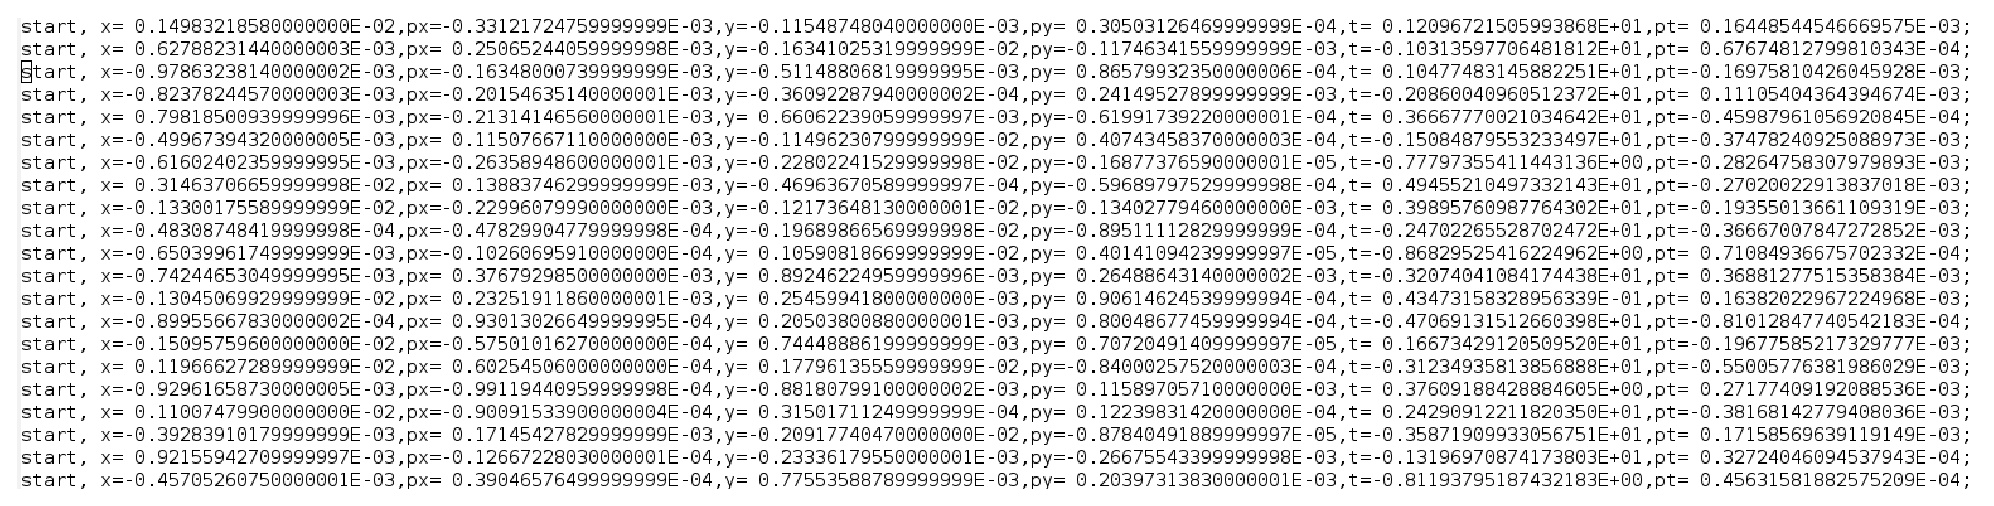
\includegraphics[height=4cm]{eps/start_coordinates}
\caption{Example of a start coordinates file.}
\label{START}
\end{figure}

\subsection{Set-Up Example}\label{SETUP}

In this section it will be described how the user's MAD-X lattice will
be instrumented with thin SC kicks. As an arbitrary example we are
using the CERN PS. It uses MAD-X internal routines and a set MAD-X
control and MACRO files.

This set-up is documented at the web-site:
\href{https://cernbox.cern.ch/index.php/s/olVfNdB8RsfYaCD}{Set-up of MAD-X with Space Charge}

One finds the following directories:
\begin{enumerate}
\item{\bf Manual}\newline
  There, one will find updated versions of this manual.
\item{\bf 6D-Matched-Distribution}\newline
  This MAD-X SC implementation requires 6D linearly matched
  distributions of a couple of 1'000 macro-particles. One finds all
  tools and instructions to prepare such distributions adapted to the
  user's machine case.
\item{\bf Set-Up\_Macros}\newline
  \begin{enumerate}
    At this location one finds the following directories:
  \item{\bf PS-example}\newline
    This directory hold's a fully instantiated example run for the
    CERN PS. It has been run on the CERN lxplus system via the
    command, given that one has placed ``~mad/bin'' in the LINUX
    \$PATH environment:
    \begin{verbatim}
madx make_machine_sequence.madx | tee out_1
  \end{verbatim}
    The MAD-X executables with Space Charge can be downloaded at the
    web at:
%\htmladdnormallink{MAD-X with SC Executables}{http://frs.web.cern.ch/frs/Source/madX_SC/exec}.
%\htmladdnormallink{MAD-X with SC Executables}{https://cern.ch/madx/releases/last-rel/}.

The relevant output file is
    ``ring\_seq\_bb\_spch\_thin.madx''. This is the thin lens PS
    lattice file instrumented with SC kicks at a particular tune
    working point. This file is one of essential input file for
    the SC simulation together with the 6D linearly matched
    distributions, as discussed above.
  \item{\bf Generic-Macros}\newline
    In this directory one finds the generic MACROs that should work
    for any machine case. In Appendix~\ref{APPENDIX2} the input file
    ``madx\_spch\_input.madx'' is explained that allows the standard
    user to modify a title in the Set-Up procedure. More relevant is
    the main input file ``make\_machine\_sequence.madx'' which is
    discussed in Appendix~\ref{APPENDIX3}. Basically, this file
    consist of a part 1 where the user is required to set-up and
    simplify the lattice of the particular machine case to be
    studied. This is followed by part 2 where, after some standard
    MAD-X commands, the user is required to specify the machine
    parameters like ``kinetic\_energy\_gev'' and 2 MACRO control
    parameters explained in the Appendix. Last, for reference of the
    purpose of the applied MACROs in Appendix~\ref{APPENDIX4} the file
    ``main\_make\_spch.madx'' is shown. The standard user will not be
    required to change anything in that file.
  \end{enumerate}
\end{enumerate}

\subsection{Run Example}

In Fig.~\ref{RUN_EXAMPLE} the SC tracking part of a typical runs is
depicted:
\begin{itemize}
\item In a first step the TFS tables {\bf time\_var\_mul} for time
  varying multipoles are read-in (see Fig.~\ref{TIME_VAR_MUL}). The
  first column has the element name, the second is the running number
  of different multipoles. In this case there are 3 different
  sextupoles. The next column gives the number of turns after which
  the multipole strength will be changed. If turn numbers are missing
  no change of the multipoles will be applied for those turn
  numbers. The following 20 columns are reserved for multipoles of up
  to $10^{th}$ order. The normal coefficients are followed by the skew
  ones: i.e. normal dipole, vertical dipole, normal quadrupole, skew
  quadrupole, normal sextupole etc. In this example the normal
  sextupoles (fifth multipole column) hold values different from
  zero. The remaining 15 columns are not shown.

  Then the TFS table of phase trombone {\bf time\_var\_pha} is read-in
  (see Fig.~\ref{TIME_VAR_PHA}). It has the same structure as the TFS
  table for multipoles. However, in this case the 36 matrix elements
  are contained in this table (32 columns have been suppressed in the
  figure). In this example there is only one phase trombone.

  This example contains no time varying cavity. The {\bf
    time\_var\_cav} file would just have the necessary first 3 columns
  and a single column with the desired {\bf VOLT} in [MV].
\item Notice that after any TWISS command one has to read-in the table
  {\bf  spch\_bb\_twiss\_ini.dat}.
\item A set of flags are needed to activate the SC treatment.
\item The MAD-X {\bf TRACK} environment is being opened and the start
  coordinates are being read-in.
\item On the MAD-X {\bf RUN} command special care has been taken to
  avoid numerical exception by defining the RF bucket.
\item A run with a single turn is followed by a loop of runs with a
  TWISS parameter recalculation after every turn at all positions of
  the SC elements. Notice, that the table {\bf
    spch\_bb\_twiss\_ini.dat} has to be read-in after each TWISS command.
\item Last, the tracking output is written out for the emittance
  evolution, the final TWISS parameters, the 6D coordinate printout
  and the record of lost particles respectively.
\item Fig.~\ref{RUN_EXAMPLE_3D} shows a {\bf RUN EXAMPLE} available
  in the implementation after 2018 featuring the flags {\bf
    sc\_3d\_kick}, {\bf sc\_3d\_periodic=TRUE} (``periodic'' mode) and
    {\bf sc\_3d\_periodic=false} (``free'' mode), see above for more
    details.

\end{itemize}

%\newpage
\begin{figure}[H]
\centering 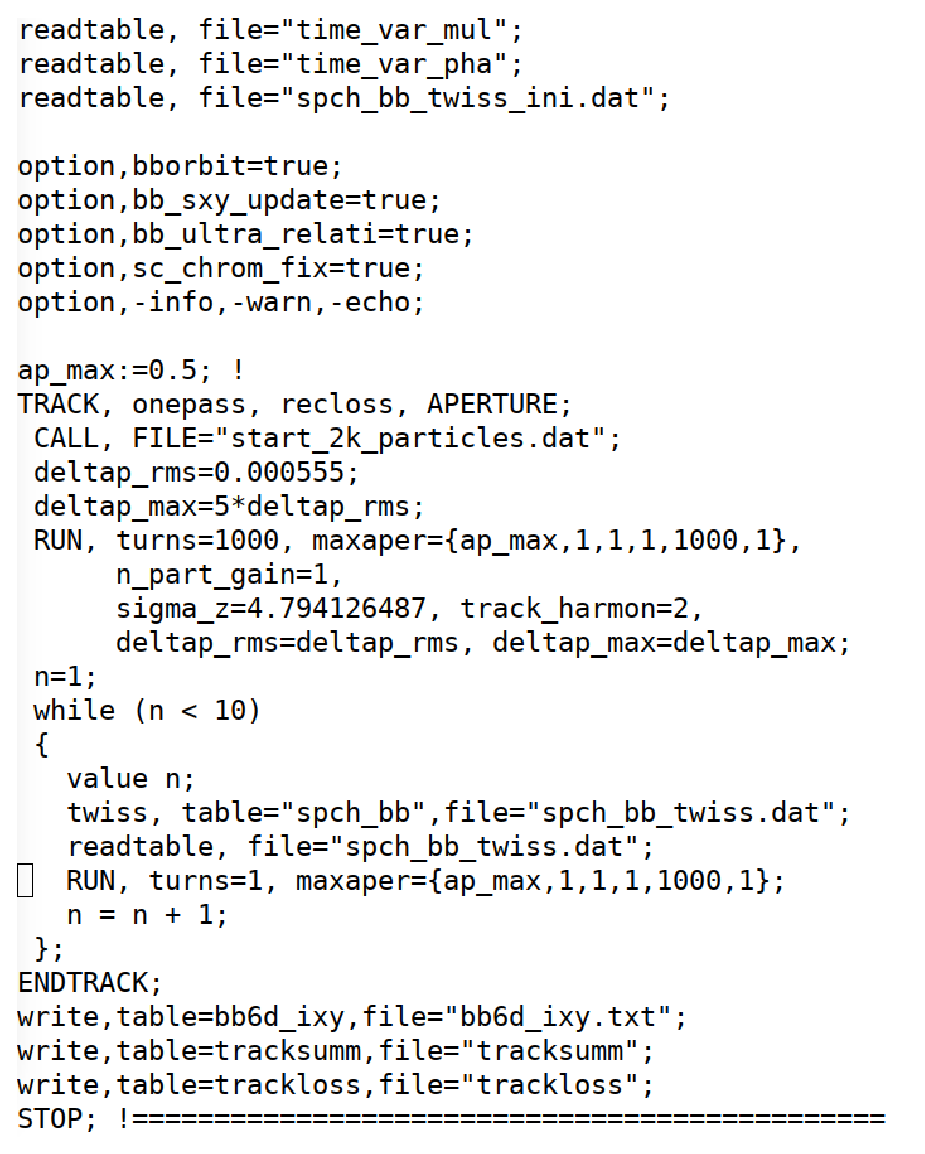
\includegraphics[width=8cm]{eps/run_example2_new}
\caption{A typical run example before the 2018 implementation,
  i.e. adaptive and purely frozen mode.}
\label{RUN_EXAMPLE}
\end{figure}

\newpage
\begin{figure}[H]
\centering 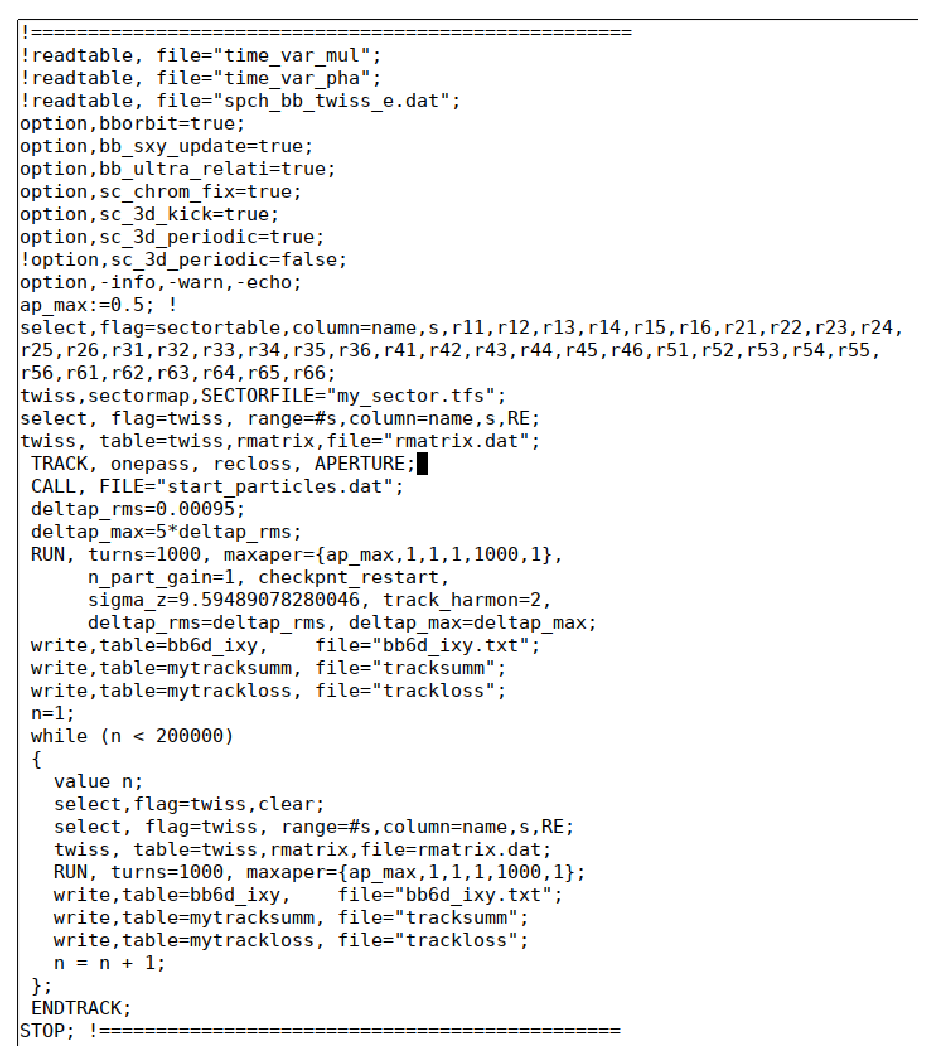
\includegraphics{eps/run_example_3D2_new}
\caption{A typical run example after 2018 implementation,
  i.e. with the symplectic SC 3D kick and ``periodic'' or
  ``free''(self-consistent) mode.}
\label{RUN_EXAMPLE_3D}
\end{figure}

\newpage
\begin{figure}[H]
\centering
\begin{minipage}[b]{0.45\linewidth}
  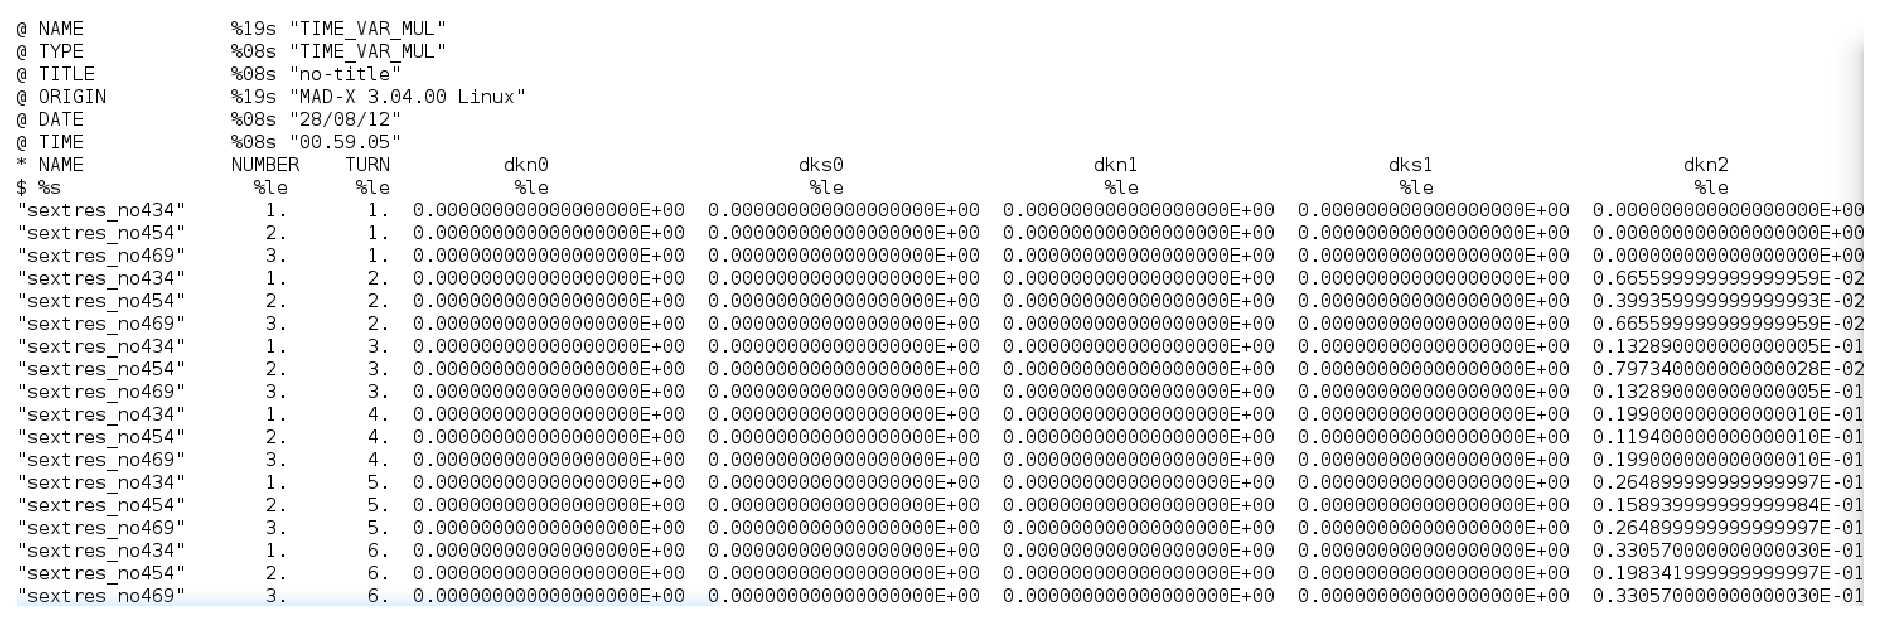
\includegraphics[height=7cm,angle=-90]{eps/cut_out_time_var_mul}
\caption{Example of a Time Variation Multipole TFS table.}
\label{TIME_VAR_MUL}
\end{minipage}
\quad
\begin{minipage}[b]{0.45\linewidth}
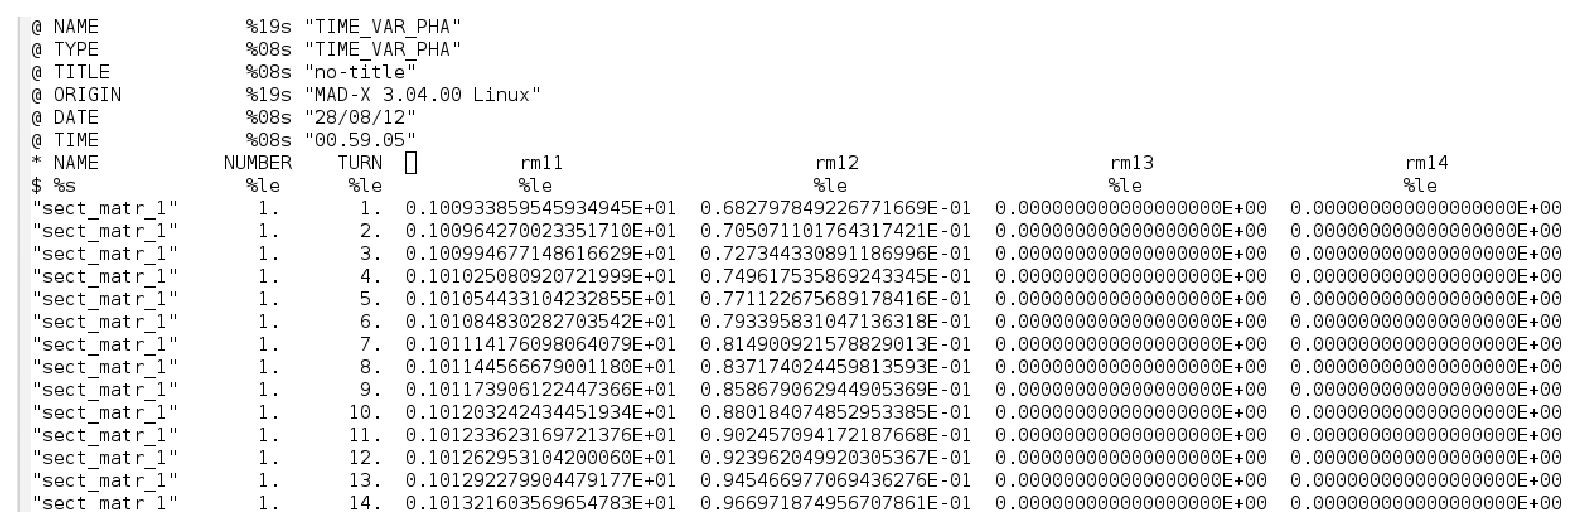
\includegraphics[height=7cm,angle=-90]{eps/cut_out_time_var_pha}
\caption{Example of a Time Variation Phase Trombone TFS table.}
\label{TIME_VAR_PHA}
\end{minipage}
\end{figure}

\subsection{Laslett Tune Shift Formulae}\label{SEC:LASLETT}

Here the formula as used in the file {\bf
  spcharge\_laslett\_tune\_shift.madx} in the third step of the
preparatory phase-I, with the tunes from TWISS:
\begin{equation}
\nu_{x, y},
\end{equation}
averaged $\bar{\beta}$ value and length of the machine
$L_{\textrm{ring}}$ relate:
\begin{equation}
\bar{\beta}_{x, y} = \frac{L_{\textrm{ring}}}{2\pi\nu_{x, y}},
\end{equation}
and averaged $\bar{\sigma}$:
\begin{equation}
\bar{\sigma}_{x, y} = \sqrt{\epsilon_{x, y}\bar{\beta}_{x, y}},
\end{equation}
the SC tune-shift reads:
\begin{equation}\label{LASLETT}
\Delta\nu_{x, y} = \frac{r_pN_p \cdot \bar{\beta}_{x, y}}{2\pi\cdot
  B_f \cdot \gamma^3 \beta^2 \cdot \bar{\sigma}_{x, y}(\bar{\sigma}_x
  + \bar{\sigma}_y)},
\end{equation}
with $B_f$ as the bunching factor.\\ \mbox{ }\\ For the particular
case of bunched Gaussian beams the SC tune shift formula reads as
follows:
\begin{equation}\label{LASLETT-BUNCH}
\Delta\nu_{x, y} = \frac{r_pN_p}{(2\pi)^{\frac{3}{2}} \cdot \gamma^3
  \beta^2 \cdot \sigma_z}\cdot \oint{\frac{\beta_{x, y}(s) \cdot
    ds}{\sigma_{x, y}(s)(\sigma_x(s) + \sigma_y(s))}}.
\end{equation}
After integration one gets:
\begin{equation}
\Delta\nu_{x, y} = \frac{r_pN_p \cdot \bar{\beta}_{x,
    y}}{(2\pi)^{\frac{3}{2}} \cdot \gamma^3 \beta^2 \cdot
  \frac{\sigma_z}{L_{\textrm{ring}}} \cdot \bar{\sigma}_{x,
    y}(\bar{\sigma}_x + \bar{\sigma}_y)}.
\end{equation}
The bunching factor can be defined as the ratio of the ``effective
length'' $L^{\textrm{eff}}_{\textrm{bunch}}$ to the length of the ring
$L_{\textrm{ring}}$.
\begin{equation}
B_f = \frac{L^{\textrm{eff}}_{\textrm{bunch}}}{L_{\textrm{ring}}}.
\end{equation}
where the "effective" bunch length can be seen as the length of an
ideal bunch with uniform distribution, which contains the same number
of particles as a bunch with an arbitrary non-uniform distribution,
e.g. a Gaussian bunch.

This implies that for Gaussian beams with the
$L^{\textrm{eff}}_{\textrm{bunch}} = \sqrt{2\pi} \cdot \sigma_z$ the
bunching factor $B_f$ should read:
\begin{equation}\label{BF}
B_f = \sqrt{2\pi} \cdot \frac{\sigma_z}{L_{\textrm{ring}}}.
\end{equation}

\subsection{Beam Modes}
Remarks on the transition from coasting to non-monochromatic and then
to bunched beams.

Demonstrated with a numerical example for the FNAL
debuncher~\cite{KAPIN-I}:
\begin{itemize}
\item[1.)]  For {\bf coasting} 4D beam $N=1.75\cdot10^{13}$ with a
  tune shift of $\Delta\nu=-0.0148$ there is a good agreement between
  the analytic Laslett's tune shift (at $B_f=1$) and the numerical
  TWISS determination.

\item[2.)]  For non-monochromatic beams in the debuncher, let's take
  into account the well-known Formulae for the beam size in the arcs
  with ($D>0$) for bunches with significant momentum
  spread~\cite{MACKEY}:
  \begin{equation}\label{DISP}
    \sigma^2_{tot}= \sigma^2_\beta + [D_x(s) \sigma_p]^2.
  \end{equation}
  With ($\sigma_p=4.5\cdot10{-3}$) and due to the large $D_x$ the tune
  shift reduces to ($\Delta\nu=-0.0054$). This value has been
  calculated numerically via MAD-X with both TWISS commands using Eq.~\ref{DISP}
  and TBT tracking over 1024 turns. Therefore, one should increase
  Npart for SC-elements by a factor of $N\_part\_gain=2.7$, i.e. by
  $\frac{0.0148}{0.0054}$, to get back ($\Delta\nu=-0.0148$) as for
  non-monochromatic beams.
\item[3.)] Number of particles in coasting and bunched beam producing
  the same Laslett tune shift:
  \begin{equation}
    \begin{split}
      Npart(6D)= Npart(4D, B_f=1) * N\_part\_gain * B_f=\\ Npart(4D,
      B_f=1) * N\_part\_gain *
      (\sqrt{2\pi}*\sigma_z/L_{\textrm{ring}})=\\
1.75\cdot10^{13}*(2.7)*(2.5*12/505)=2.8\cdot10^{12}.
  \end{split}
  \end{equation}
\end{itemize}
\subsubsection{General MAD-X Set-Up Input}\label{APPENDIX2}
The user may modify the input file ``madx\_spch\_input.madx''. In
particular the {\it\bf title\_madx\_script} entry maybe modified to
the user's taste: it will appear in MAD-X output files during the
Set-Up phase and does not alter the outcome otherwise. Changing the
other two items is discouraged and should only be performed by experts
since it will require various other changes in the generic MACROS.
\begin{verbatim}
*****************************************************************************
input file: madx_spch_input.madx:
********************************
&input_filename
twiss_element_list_filename='twiss_element_list.txt'
                 ! created in 1a_step
&END

&madx_job_title
title_madx_script='2021: PS Run'
&END

&ring_seq_filename
filename_ring_elements_seq='machine_sequence.madx'
                       ! ring sequence with SAVE, SEQUENCE=<>,file=<>.madx;
&END
*****************************************************************************
\end{verbatim}

\subsubsection{Preparing MAD-X Lattice for SC Kicks}\label{APPENDIX3}
The main input file ``make\_machine\_sequence.madx'' consist of a
user defined simplified original lattice definition of the user's
machine case. This part is followed by some generic MAD-X commands
and a list of input parameters that the user needs to adapt to his case.
This second part of the file is depicted below. Besides evident
parameters like ``kinetic\_energy\_gev'' there are 2 relevant
parameters:
\begin{enumerate}
\item{\bf L\_div\_max}\newline
  This parameter defines the maximum distance between 2 SC kicks in
  [m]. For the PS we have been using 1 [m] which has allowed for a
  dense enough coverage of SC kicks around the machine and about 1'100
  kicks seems good enough. Obviously, one should not overdo the number
  of kicks because this number is directly proportional to the
  execution time of the run. As an example: for the PS 500'000 turns
  take about 6 weeks computing time on modern computer PCs.
\item{\bf delta\_nu\_min}\newline
  The MAD-X SC Set-Up procedure is turning on the strength of the SC
  kicks adiabatically to avoid potential TWISS command crashes because the
  strength of the SC kicks depend on the TWISS parameters itself. The
  {\it\bf delta\_nu\_min} parameter controls the speed of the
  convergence. Typically we are using {\it\bf delta\_nu\_min=0.25} but
  for the PS we needed to do it in finer steps: {\it\bf
    delta\_nu\_min=0.07}.
\end{enumerate}
\begin{verbatim}
*****************************************************************************
input part of file: make_machine_sequence.madx:
***********************************************
!
! Create file=twiss_element_list.txt printing element list
 SELECT, flag=twiss,clear;
 SELECT, flag=twiss, column=name, keyword, L;
 TWISS, file=twiss_element_list.txt;

! Do former "2_step MAD-X SC internally
 option,sc_setup=true; ! required do not change
 TWISS;
 option,sc_setup=false; ! required do not change

! Write out the machine sequence as file=machine_sequence.madx
 SAVE,SEQUENCE=MACHINE,file=machine_sequence.madx;
 call,file=machine_sequence.madx;

!
!Machine Parameters: Example PS
!
!Parameters to be set
kinetic_energy_gev =   2.0 ;
Ex_norm=3.5E-6 ; ! Normalized horizontal emittance
Ey_norm=2.2E-6 ; ! Normalized vertical emittance
Bunch_length_4s=135e-9 ; ! 4 sigma bunch_length [ns]
NPART_tot=55e10 ; ! Total number of particles in the machine
L_div_max=1.; value, L_div_max;  ! Upper limit for segment length
delta_nu_min=0.07; ! Typical 0.25; ! FRS 02.09.2020 Constant for tune-shift of PS

L_ring:=table(summ,length);
value, L_ring;
rest_energy_gev =   pmass ;
total_energy_GeV:=kinetic_energy_GeV+rest_energy_GeV;
gamma=total_energy_GeV/rest_energy_gev;
beta=sqrt(1.-1./gamma^2);
value, gamma,beta;
Ex_spch:=Ex_norm/gamma/beta; Ey_spch:=Ey_norm/gamma/beta; ! [m] ! PS tracking
Bunch_length:= Bunch_length_4s/4.*clight*beta; ! PS 1 RMS bunchlength in [m]
value,Bunch_length, clight, beta;
NPART:=NPART_tot*L_ring/Bunch_length/sqrt(2*pi); ! PS new definition
value, NPART;
N_spch:=SC_count-1;
value, L_div_max,N_spch,SC_count,delta_nu_min;

! EXPERTS Usuage only! Needed for backwards compatibility mode
CALL, FILE=input_compatibility.madx; ! required do not change

! Do former "3_step" with generic MACROs
CALL, FILE=main_make_spch.madx; ! required do not change
stop;
*****************************************************************************
\end{verbatim}

\subsubsection{Adiabatic Switching on SC}\label{APPENDIX4}
The execution of the MACROs is controlled by the file
``main\_make\_spch.madx''. There is no need to modify this file by
the standard user. It is just shown for a reference of the purpose of
each individual MACRO.
\begin{verbatim}
*****************************************************************************
input file: main_make_spch.madx:
*******************************
! Start file: "main_make_spch.madx"
! Calling MACROS
option,info,warn,echo,bb_ultra_relati;
set,format="24.16e";
debug_print=0;

value,rest_energy_GeV,kinetic_energy_GeV,total_energy_GeV,clight,gamma,
beta,Bunch_length,N_particles,Z_particle,A_particle,r0_particle,prad,L_div_max;

CALL FILE=spcharge_macro_20090316.madx;

! backwards compatibility mode
!CALL FILE=spcharge_constants_and_formulae.madx; ! <= constants for space charge

! backwards compatibility mode
!CALL FILE=spcharge_input_parameters.madx; ! <=input parameters for space charge

Call FILE=spcharge_beam_command.madx;     ! BEAM command

CALL FILE=spcharge_ring_seq.madx;       ! <= read lattice sequence
                                        ! with universal name (file generated by CVF)

USE, PERIOD=ring; TWISS;

Call FILE=spcharge_beam_command.madx;     ! second BEAM command

! =====  Analytical  tune shift ===============================
CALL FILE=spcharge_laslett_tune_shift.madx; ! <= Analytical evaluation 

debug_print=0;

CALL FILE=spcharge_matrix.madx;

debug_print=0;

CALL FILE=spcharge_bbkick.madx;

! MAKETHIN
CALL, FILE = spcharge_makethin.madx;

twiss;
emit;
stop;
! End file: "main_make_spch.madx"
! End MAD-X file "make_machine_sequence.madx"
\end{verbatim}
*****************************************************************************

%% EOF
     % THINTRACK: Thin-Lens Tracking Module 

\part{\ptc Commands}
%%\title{PTC Set-up Parameters}
%  Created by: Valery KAPIN, 21-Mar-2006
%  Changed by: ____________, ___________

\chapter{\ptc Set-up Parameters}
\label{chap:ptc-setup}

The Polymorphic Tracking Code \cite{forest2002} of Etienne
Forest is a kick code, allowing a symplectic integration through all
accelerator elements giving the user full control over the precision
(number of   steps and integration type) and exactness (full or extended
Hamiltonian) of the   results.
The degree of exactness is determined by the user and the speed of his
computer.
The main advantage is that the code is inherently based on the map
formalism and provides users with all associated tools.

The \ptc code is actually a library that can be used in many different
ways to create an actual module that calculates some property of
interest.

\textbf{Attention:}
\ptc exists inside of \madx as a library. \madx offers the interface to
\ptc, \textsl{i.e.} the \madx input file is used as input for \ptc.
Internally, both \ptc and \madx have their own independent databases
which are linked via the interface. With the
\hyperref[sec:ptc-create-layout]{\texttt{PTC\_CREATE\_LAYOUT}} command,
only numerical values are transferred
from the \madx data structures to the \ptc data structures. Any
modification to the \madx data structure is unknown to \ptc until the
next call to \hyperref[sec:ptc-create-layout]{\texttt{PTC\_CREATE\_LAYOUT}}.
For example, a \hyperref[sec:defer]{deferred expression} of \madx is
only evaluated at the time of the
\hyperref[sec:ptc-create-layout]{\texttt{PTC\_CREATE\_LAYOUT}} command and
is ignored within \ptc afterwards.


Several modules using the PTC code have been presently implemented in
\madx. These {\madx}-{\ptc} modules\cite{schmidt2005} are executed by
the following commands:
\hyperref[chap:ptc-twiss]{\texttt{PTC\_TWISS}},
\hyperref[chap:ptc-normal]{\texttt{PTC\_NORMAL}},
\hyperref[chap:ptc-track]{\texttt{PTC\_TRACK}},
\hyperref[sec:ptc-trackline]{\texttt{PTC\_TRACK\_LINE}}.

To perform calculations with these {\madx}-{\ptc} commands, the \ptc
environment must be initialized, handled and turned off by special
commands within the \madx input script.

\section{Command Synopsis}
\label{sec:ptc-synopsis}

A typical set of commands to invoke \ptc is given below:

\madxmp{
PTC\_CREATE\_UNIVERSE, \=SECTOR\_NMUL\_MAX= integer, SECTOR\_NMUL= integer,  \\
                       \>NTPSA= logical, SYMPRINT= logical; \\
\\
PTC\_CREATE\_LAYOUT, \=TIME= logical, MODEL= integer, \\
                     \>METHOD= integer, NST= integer, EXACT= logical, \\
                     \>OFFSET\_DELTAP= double, ERRORS\_OUT= logical, \\
                     \>MAGNET\_NAME= string, RESPLIT= logical,  \\
                     \>THIN= double, XBEND= double,  \\
                     \>EVEN = logical; \\
... \\
PTC\_MOVE\_TO\_LAYOUT, INDEX= integer; \\
...\\
PTC\_READ\_ERRORS, OVERWRITE= logical; \\
... \\
PTC\_ALIGN; \\
...\\
PTC\_END;
}

\section{PTC\_CREATE\_UNIVERSE}
\label{sec:ptc-create-universe}

The \texttt{PTC\_CREATE\_UNIVERSE} command is required to set-up the
\ptc environment.

\madbox{
PTC\_CREATE\_UNIVERSE, \=SECTOR\_NMUL\_MAX=integer, SECTOR\_NMUL=integer, \\
                       \>NTPSA=logical, SYMPRINT=logical;
}

The attributes are:
\begin{madlist}

   \ttitem{SECTOR\_NMUL\_MAX} a global variable in \ptc needed for exact
   sector bends defining up to which order Maxwell's equation are solved
   (see \cite{forest2002}~page~76-77).
   The value of \texttt{SECTOR\_NMUL\_MAX} must not be smaller than
   \texttt{SECTOR\_NMUL} otherwise \madx stops with an error.
   If a negative value is passed than it is identified automatically
   by scanning the currently selected sequence.
   \\ (Default:~-1)

   \ttitem{SECTOR\_NMUL} a global variable in PTC needed for exact
   sector bends defining up to which order the multipole are included in
   solving Maxwell's equation up to order \texttt{SECTOR\_NMUL\_MAX}.
   Multipoles of order N with N $>$ \texttt{SECTOR\_NMUL} and N $\leq$
   \texttt{SECTOR\_NMUL\_MAX} are treated similar to \textit{SixTrack}.
   If a negative value of \\
   \texttt{SECTOR\_NMUL\_MAX} is passed than it is also identified automatically.
   However, if multipolar parameters of the bends are to be modified inside the PTC universe,
   for example with \texttt{PTC\_READ\_ERRORS},
   then this parameter needs to be set to a corresponding value.
   Please note that using large values (above 10) slows down the computations,
   so the smallest required value should be used. We recommended a minimum of
   MAX(\texttt{ORDER}+1,N+2) (where \texttt{ORDER} is the order of the map), 
   however \texttt{order}+1+N would give the most accurate results. \\
   (Default:-1)

   \ttitem{NTPSA} invokes the Differential Algebra (DA) package
   written in C++ and kindly provided by Lingyun Yang (lyyang@lbl.gov). \\
   Etienne Forest has written the wrapper to allow the use of both
   the legendary DA package written in Fortran by Martin Berz
   (default) and this new DA package of Lingyun~Yang.
   It is expected that this DA package will allow for the efficient
   calculation of a large number of DA parameters. \\ (Default:~false)

   \ttitem{SYMPRINT} a flag to enable the printing of the check of
   symplecticity. It is recommended to leave this flag set to TRUE. \\
   (Default: true)
\end{madlist}


\section{PTC\_CREATE\_LAYOUT}
\label{sec:ptc-create-layout}

The \texttt{PTC\_CREATE\_LAYOUT} command creates the \ptc-layout
according to  the specified integration method and fills it with the
current \madx sequence defined in the latest
\hyperref[sec:use]{\texttt{USE}} command.

\madbox{
PTC\_CREATE\_LAYOUT, \=TIME=logical, MODEL=integer, METHOD=integer,  \\
                     \>NST=integer, EXACT=logical, OFFSET\_DELTAP=double, \\
                     \>ERRORS\_OUT=logical, MAGNET\_NAME=string, \\
                     \>RESPLIT=logical, THIN=double, XBEND=double, \\
                     \>EVEN=logical;
}

The attributes are:
\begin{madlist}

  \ttitem{TIME} a logical flag to control which coordinate system
  is being used. \\ (Default=~true) \\ \\
  Please see \texttt{TIME} of \hyperref[sec:ptc-setswitch]{\texttt{PTC\_SETSWITCH}}
  command for more details.

  \ttitem{MODEL} an integer to switch between models:\\
  1 for "Drift-Kick-Drift";  (Default value)\\
  2 for "Matrix-Kick-Matrix" and \\
  3 for "Delta-Matrix-Kick-Matrix" (SixTrack-code model). \\
  Note: Model 1 usually will require more integration and slicing than model 2.

  \ttitem{METHOD} the integration order: 2, 4, 6 or 8. This will either use
  Forest-Yoshida integration or Boole's rule (See \cite{forest2002}~Chapter~K for 
  more details). The optimum \texttt{METHOD} value corresponds to
  the value beyond which the studied properties no longer change 
  (in conjunction with increasing slicing). \texttt{METHOD} has a greater effect
  on this convergence, while not increasing the amount of computations as much 
  as slicing would to achieve the same convergence \\ (Default: 2)

  \ttitem{NST} the number of integration steps.  (Default:~1)\\
  The body of each element is divided into \texttt{NST} equal slices and
  Forest-Yoshida integration is carried out on each slice.
  For best results \texttt{NST} should increase with strength
  and length of elements. The optimum \texttt{NST} value corresponds to
  the value beyond which the studied properties no longer change.
  However, for time consuming calculations the user may
  reduce \texttt{NST}. (See below the \texttt{RESPLIT} option for automatic
  adjustment.)\\
  This attribute sets the same \texttt{NST} value  for all "thick" elements
  ($l > 0$) of a beam-line; however each individual element may also have
  its own \texttt{NST} value defined independently
  (\hyperref[sec:add-option-PTC]{see below}).

  \ttitem{EXACT} a logical flag to turn on calculations with an exact
  Hamiltonian, otherwise the expanded Hamiltonian is used. \\
  (Default:~false)

  \ttitem{OFFSET\_DELTAP} \textbf{[ Beware: Expert attribute! ]}
  provides relative momentum deviation of the reference particle (6D case
  ONLY). This option implies \texttt{TOTALPATH=true}. \\
  (Default: 0.0)

  \ttitem{ERRORS\_OUT} a logical flag to write-out multipolar errors
  in \hyperref[sec:efcomp]{\texttt{EFCOMP}} table format.
  \\ (Default: false) \\
  Two tables are created and filled: "errors\_field" contains only
  field errors, "errors\_total" contains also desired field
  components, which can include the strength of correctors.
  The choice of magnets is defined by the \texttt{MAGNET\_NAME}
  attribute (see below).
  The tables can be \hyperref[sec:write]{written} to file, and can be
  read back via the \texttt{ERRORS\_IN} flag.\\
  The \texttt{ERRORS\_IN} flag has precedence over this \texttt{ERRORS\_OUT} flag.

  \ttitem{MAGNET\_NAME} a string giving a simple selection for the
  names of magnet to be used for an error write-out using the
  \texttt{ERRORS\_OUT} flag (see above). The errors are recorded for all
  magnets with names starting with the exact string given here, which
  would be equivalent to the ??? regular expression.\\
  (Default:~nil)

  \ttitem{RESPLIT} a logical flag to apply the \ptc resplit
  procedure. This is meant to create an "adaptive" setting of the
  \texttt{METHOD} and \texttt{NST} attributes according to the strengths
  of quadrupoles (using the \texttt{THIN}  attribute) and dipoles (using
  the \texttt{XBEND} attribute). The \texttt{EVEN} attribute further
  controls the number of splits.  \\
  (Default:~false)

  \ttitem{THIN} is the main \texttt{RESPLIT} attribute and is meant for
  splitting quadrupoles according to their strength. The default value
  \texttt{THIN=0.001} has shown in practice to work well without costing
  too much with respect of performance.

  \ttitem{XBEND} is an optional \texttt{RESPLIT} attribute and is meant for
  splitting dipoles. A value \texttt{XBEND=0.001} is also advisable for
  dipoles. \\
  (Default: -1.0 for no splitting)

  \ttitem{EVEN} a logical switch to ensure even number of splits when
  using the \texttt{RESPLIT}  procedure of \ptc, which is particularly
  useful when one attempts to calculate \texttt{PTC\_TWISS} with the
  \texttt{CENTER\_MAGNETS} option, i.e. to calculate the \texttt{TWISS}
  parameters in the center of the element.
  Uneven number of splits is ensured with \texttt{EVEN=false}.
  (Default:~true)
\end{madlist}

\section{PTC\_SETSWITCH}
\label{sec:ptc-setswitch}

The \texttt{PTC\_SETSWITCH} command allows to set some global \ptc states and to configure the interface between {\madx} and {\ptc}, adapting the behavior of the program to the needs.

\madbox{
	PTC\_SETSWITCH, \=DEBUGLEVEL=integer, MAPDUMP=integer, MADPRINT=logical, \\
	\>EXACT\_MIS=logical, TOTALPATH=logical, RADIATION=logical, \\
	\>ENVELOPE=logical, STOCHASTIC=logical, MODULATION=logical,\\
	\>FRINGE=logical, TIME=logical, SEED=integer, \\
  \>MAXACCELERATION=logical, NOCAVITY=logical, NOCHARGE=logical;
}

The command parameters and switches are:
\begin{madlist}
	\ttitem{DEBUGLEVEL} (Default: 1)\\
	Sets the level of debugging printout: 0 prints none, 4 prints everything

  \ttitem{MAPDUMP} (Default: 0)\\
  Sets the level of map dump printout in all tracking codes. \\
  0: None,\\
  1: Order 0,\\
  2: Order 1,\\
  3: The full map.

  \ttitem{MADPRINT} (Default: false)\\
  Sets map dump printout format so that it can be read by MAD-NG

	\ttitem{EXACT\_MIS} (Default: false)\\
	Switch ensures exact misalignment treatment.

	\ttitem{TOTALPATH} (Default: false)\\
	If true, the 6th variable of PTC, i.e. 5th of MAD-X, is the total path.  \\
	If false it is deviation from the reference particle,
	which is normally the closed orbit for closed layouts. \\
	This switch changes behaviour of the RF cavities,
	including RF multipoles and crab cavities.
	If it is false, the time of flight effect between the cavities
	(or the ring length) is ignored because the kick is proportional to \\
	$sin(2\pi \cdot \rm{FREQ} \cdot t/c + \rm{LAG})$, where $t$ is the time coodinate.
	So only distance from the synchronous particle plays a role.
	For example, changing ring length will not affect the cavity.
	On the other hand, it gurantees that the defined LAG is observed.
	Conversely, if \texttt{TOTALPATH} is true then $t$ becomes the total time of flight
	so its effect is accounted for. In the case when cavity is detuned
	the closed orbit momentum will change and in ray tracking phase slippage from turn
	to turn will be seen. However, \texttt{LAG} of cavities needs to be
	carefuly calculated because its phasing will depend on its position.
	Naturally, in cases with only one RF cavity the closed orbit search will automatically
	determine the offset.

	\ttitem{RADIATION} (Default: false)\\
	Sets the radiation switch/internal state of PTC. In PTC basically all the elements
	radiate including sextupoles, solenoids and orbit correctors.

	\ttitem{ENVELOPE} (Default: false)\\
	Sets the envelope switch/internal state of PTC. It allows to calculate
	dumping due to radiation and stochastic effects.
	Warning: this makes the tracking approximately twice slower, so low order
	should be used.

	\ttitem{STOCHASTIC} (Default: false)\\
	Sets the stochastic switch/internal state of PTC.
	It enables stochastic emission of photons in ray tracking,
                    it only affects \texttt{PTC\_TRACK} and \texttt{PTC\_TRACKLINE}.
	The emission is calculated during map tracking therefore
	\texttt{PTC\_TWISS} or \texttt{PTC\_NORMAL}
	needs to be invoked before launching the tracking
	(also with \texttt{RADIATION}, \texttt{ENVELOPE} and \texttt{STOCHASTIC} set to true).
	Every tracked ray will receive the same stochastic kicks.

	\ttitem{MODULATION} (Default: false)\\
	Sets the modulation switch/internal state of PTC.
	It needs to be set to true to observe effect of AD dipoles.

	\ttitem{FRINGE} (Default: false)\\
	Sets the fringe switch/internal state of PTC. \\
	If true the influence of the fringe fields is evaluated for quadrupole fringe fields based on the $b_2$ and $a_2$ components of the element.

	Please note that currently fringe fields are always taken into
	account for some elements (e.g. traveling wave cavities) even if
	this flag is set to false. The detailed list of elements
	will be provided later, when the situation in this matter will be
	definitely settled.

	\ttitem{TIME} (Default: true)\\
	If true, Selects time of flight (\textit{cT} to be precise) rather
	than path length as the 6th variable of PTC, i.e. 5th of MAD-X. \\
                    This option changes the canonical coordinate system depending
	whether the calculation is done in 5D or 6D:
	 \begin{madlist}
	   \ttitem{5D} if \texttt{TIME} is true, the fifth coordinate is
	   \hyperref[subsec:tables-canon]{\texttt{PT}},
	   $p_t = \Delta E / p_0 c$ \\
	   if \texttt{TIME} is false, the fifth coordinate is
	   \hyperref[subsec:tables-canon]{\texttt{DELTAP}},
	   $\delta_p = \Delta p / p_0$

	   \ttitem{6D} if \texttt{TIME} is true, the
	   \hyperref[subsec:tables-canon]{\madx coordinate system}
	   \{$-ct$, $p_t$\} is used. \\
	   if \texttt{TIME} is false, the second \ptc coordinate system
	   \{-pathlength, $\delta_p$\} is used.
	 \end{madlist}

	\textbf{Note:} at small energy ($\beta_0 << 1$),
	momentum-dependent variables like dispersion will depend  strongly on
	the choice of  the logical input variable \texttt{TIME}. In fact, the
	derivative ($\frac{\partial}{\partial \delta_p}$)  and
	($\frac{\partial}{\partial p_t}$)  are different by the
	factor $\beta_0$. One would  therefore typically  choose
	the option \texttt{TIME=false},  which sets the fifth variable to
	the relative momentum deviation $\delta_p$.


	\ttitem{SEED} (Default: 123456789)\\
	Sets the seed of PTC random number generator,
	which is independent from the MADX generators.

	\ttitem{MAXACCELERATION} (Default: true)\\
	Switch to set cavities phases so the reference orbit is always on
	the crest, i.e. gains max energy.

  \ttitem{NOCAVITY} (Default: false)\\
  Switch to turn off the RF cavities, with \texttt{NOCAVITY=true}, 
  RF cavities are ignored.

  \ttitem{NOCHARGE} (Default: true)\\
  Switch to ignore the charge of your beam. If set to false, 
  the charge of the beam is taken into account.


\end{madlist}

%% \textbf{PROGRAMMERS MANUAL}
%% Values of the switches are stored in Fortran 90 module
%% mad\_ptc\_intstate (mad\_ptc\_intstate.f90). The command is processed by
%% pro\_ptc\_setswitch C function, in file madxn.c, that calls appropriate
%% routines of the Fortran module to set each of the switches:
%% \begin{itemize}
%%    \item  ptc\_setdebuglevel
%%    \item  ptc\_setaccel\_method
%%    \item  ptc\_setexactmis
%%    \item  ptc\_setradiation
%%    \item  ptc\_settotalpath
%%    \item  ptc\_settime
%%    \item  ptc\_setfringe
%% \end{itemize}

\section{PTC\_MOVE\_TO\_LAYOUT}
\label{sec:ptc-move-to-layout}

Several \ptc layouts can be created within a single \ptc-"universe".
The layouts are automatically numbered with sequential integers by the
\madx code. The \texttt{PTC\_MOVE\_TO\_LAYOUT} command is used to
activate a specific layout, and the next \ptc commands will be
applied to this active \ptc layout until a new \ptc layout is created
or activated.

\madbox{
PTC\_MOVE\_TO\_LAYOUT, INDEX=integer;
}

The only attribute is:
\begin{madlist}
	\ttitem{INDEX} is the numeric index of the \ptc layout to be
	activated.\\ (Default:~1)
\end{madlist}

\section{PTC\_READ\_ERRORS}
\label{sec:ptc-read-errors}

The \texttt{PTC\_READ\_ERRORS} command reads any number of
\textbf{"errors\_read"} table through the
\hyperref[sec:readtable]{\texttt{READTABLE}} mechanism.

\madbox{
PTC\_READ\_ERRORS, OVERWRITE=logical;
}

The only attribute is
\begin{madlist}
   \ttitem{OVERWRITE} a flag to specify that the read-in errors
   overwrite previous errors instead of adding the read-in errors to
   existing errors, ie multipole components already present.\\
   (Default:~false)
\end{madlist}

\textbf{Note:}\\
  For calculations with exact flag set to true,
  \texttt{SECTOR\_NMUL} parameter of \texttt{PTC\_CREATE\_UNIVERSE}
  needs to be set to a value bigger than the highest order of an error in bending magnets.

\textbf{Note:}\\
Because of the way the table is read in memory, a warning will always be
issued by default in the form:
{\small
\begin{verbatim}
warning: string_from_table_row: row out of range: errors_read->name[1>=n+1<=n]
\end{verbatim}
}
where \texttt{n} is  the number of records read from the table.
This warning has no consequence on the errors read and the following
calculation. \\
The warning is purely the result of the way that the reading loop is
programmed with a break based on the return value of the routine
\textsl{string\_from\_table\_row}.
But if \textsl{string\_from\_table\_row} tries to read in a row (\texttt{n+1})
past the last row (\texttt{n}) of the table, it prints a warning before
returning a value that will effectively break the loop. Of course this
will only happen if the \texttt{WARN} option is true and this can be turned
off with \madxmp{OPTION, -WARN;}



\section{PTC\_ALIGN}
\label{sec:ptc-align}

The \texttt{PTC\_ALIGN} command is used to apply the \madx alignment
errors to the current PTC layout, and takes no attributes.

\madbox{
PTC\_ALIGN;
}


\section{PTC\_END}
\label{sec:ptc-end}

The \texttt{PTC\_END} command turns off the \ptc environment,
which releases all memory and returns control to the \madx world proper.

\madbox{
PTC\_END;
}


\section{Additional Options for Physical Elements}
\label{sec:add-option-PTC}

For some of the \madx elements, additional attributes can be defined
that are available to \ptc only. \ptc also uses standard \madx
attributes in a slightly different way.

\madbox{
SBEND | \=RBEND | QUADRUPOLE | SEXTUPOLE | OCTUPOLE | SOLENOID ,\\
        \>L=real, ... , TILT=real, ... , NST=integer, ... ,\\
        \>KNL=\{real, real, real,...\}, KSL=\{real, real, real,...\};
}

These attributes are:
\begin{madlist}
  \ttitem{L} the length of the element. \\ \ptc treats bending magnets
  (\hyperref[sec:bend]{\texttt{SBEND}} or \hyperref[sec:bend]{\texttt{RBEND}})
  as \hyperref[sec:marker]{\texttt{MARKER}} if their length is equal to zero.

  \ttitem{NST} gives a specific \hyperref[sec:ptc-twiss]{\texttt{NST}}
  values for a particular "thick" element ($L > 0$). \\
  \\
  For example RF cavities are represented in \madx
  by a single kick, while \ptc splits the RF cavity into
  \texttt{NST} segments thereby taking into account properly the
  transit-time effects of the cavity. Specifying explicitly \texttt{NST=1}
  for RF cavity reproduces in \ptc the approximate results of \madx,
  ignoring transit time effects.
  \\

  \ttitem{KNL, KSL} The full range of  normal and skew multipole
  components on the bench can be  specified for the following physical
  elements:
  \hyperref[sec:bend]{\texttt{sbend}},
  \hyperref[sec:bend]{\texttt{rbend}},
  \hyperref[sec:quadrupole]{\texttt{quadrupole}},
  \hyperref[sec:sextupole]{\texttt{sextupole}},
  \hyperref[sec:octupole]{\texttt{octupole}} and
  \hyperref[sec:solenoid]{\texttt{solenoid}}.
  \texttt{KNL} and \texttt{KSL} multipole coefficients are specified as the
  integrated value ($\int K ds$) of the field components along the
  magnet axis. The multipole components in \ptc are spread over
  the length of thick elements. This is a considerable
  advantage of \ptc input compared  to \madx  which allows only
  \hyperref[sec:multipole]{thin multipoles}.
  \begin{madlist}
    \ttitem{KNL} is an array representing the normal multipole
    coefficients. \\ (Default:~0~m$^{-1}$)
    \ttitem{KSL} is an array representing the skew multipole
    coefficients. \\ (Default:~0~m$^{-1}$)
  \end{madlist}

  A full range of additional multipole \hyperref[sec:efcomp]{field
    errors} can be additionally specified with the
  \hyperref[sec:efcomp]{\texttt{EFCOMP}} command. Errors are added to
  the above multipole fields on the bench.\\
  If you specify the corresponding multipole coefficient in a magnet that can accept 
  a non integrated value, these are added together, i.e. 
  $\texttt{k}_1 = \texttt{k}_1 + \texttt{knl}[2]/\texttt{l}$, 
  where \texttt{knl[2]} is the value of the second element of the array knl and .

\end{madlist}

\subsection{Additional Fringe Field Parameters}

The following parameters are available for the following elements 
(Additional details can be found in \ref{sec:bend}):

\madbox{
SBEND | \=RBEND | QUADRUPOLE | SEXTUPOLE | OCTUPOLE | SOLENOID ,\\
        \>FINT=real, FINTX=real, HGAP=real, FRNGMAX=integer, \\
        \>F1=real, F2=real, FRINGE=integer, ...;
}

\begin{madlist}

  \ttitem{FINT} (Default:  0) \\
  The fringe field integral at entrance and exit of the
  bend.\\ This has been activated for all elements listed above, 
  not just for \texttt{(S|R)BEND}, as in \madx. 

  \ttitem{FINTX} (Default: =\texttt{FINT}) \\
  If defined and positive, the fringe field integral at
  the exit of the element, overriding \texttt{FINT} for the
  exit. \\
  This allows to set different fringe field integrals at entrance
  (\texttt{FINT}) and exit (\texttt{FINTX}) of the element.\\
  This has been activated for all elements listed above, 
  not just for \texttt{(S|R)BEND}, as in \madx. 

  \ttitem{HGAP} (default: 0 m) \\
  The half gap of the magnet.\\
  This has been activated for all elements listed above, 
  not just for \texttt{(S|R)BEND}, as in \madx. 

  \ttitem{FRNGMAX} (default: 2) \\
  The maximum multipole component to be included in the multipolar fringe field.

  \ttitem{F1} (default: 0) \\
  The entry linear fringe field coefficient for quadrupoles, from SAD \cite{sad_quad_2022}. \\

  \ttitem{F2} (default: 0) \\
  The exit linear fringe field coefficient for quadrupoles, from SAD \cite{sad_quad_2022}. \\
  
  \ttitem{FRINGE} (default: 0) \\
  This is a bit mask that specifies the fringe field model to be used.
  The bits are defined as follows:\\

  1: The dipole fringe field is performed using the \texttt{FINT}, 
  \texttt{FINTX} and \texttt{HGAP} parameters. 
  Note: It is not possible to remove this fringe from a bend element, as \ptc
  will always use the dipole fringe field for bending magnets.\\

  2: The multipole fringe field is performed, integrating up to the minimum of 
  \texttt{FRNGMAX} and the highest multipole component specified.\\

  4: Use the linear fringe field map for the quadrupole from the SAD code, 
  using parameters \texttt{F1}, \texttt{F2} \cite{sad_quad_2022}. \\ \\


  An example use of the \texttt{FRINGE}, would be to specify a dipole fringe and 
  the multipolar fringe field, has \texttt{FRINGE=3}, but to specify the multipolar
  fringe field and the SAD fringe field map, use \texttt{FRINGE=6}.

\end{madlist}

\subsection{Additional Pole Face Parameters}

The following parameters are available for the following elements, 
not just for \texttt{(S|R)BEND}, as in \madx 
(Additional details can be found in \ref{sec:bend}):

\madbox{
  SBEND | \=RBEND | QUADRUPOLE | SEXTUPOLE | OCTUPOLE ,\\
          \>..., E1 = real, E2 = real, ..., H1 = real, H2 = real;
}

\begin{madlist}
  \ttitem{E1} (default: 0 rad) \\
  The entry pole face rotation angle.\\

  \ttitem{E2} (default: 0 rad) \\
  The exit pole face rotation angle.\\

  \ttitem{H1} (default: 0 m$^{-1}$) \\
  The entry pole face curvature.\\

  \ttitem{H2} (default: 0 m$^{-1}$) \\
  The exit pole face curvature.\\

\end{madlist}

\subsection{Additional Parameters for the \texttt{SBEND} and \texttt{RBEND} elements}

The following parameters are available for the \texttt{SBEND} and \texttt{RBEND} elements:

\madbox {
  SBEND | \=RBEND, \\
  \>..., K0=real, K0S=real, K1=real, K1S=real, \\
  \>K2=real, K2S=real, K3=real, K3S=real, ...;  
}

The philosophy of the implementation of these components is the same as described 
in \ref{sec:add-option-PTC}, i.e. the multipole components (divided by the element length) 
are added to the strengths listed above.


\subsection{Parameters for the \texttt{CAVITY} elements}

The following parameter is available for the following elements:
\madbox{
  RFCAVITY | \=RFMULTIPOLE | CRABCAVITY, \\
  \> ..., no\_cavity\_totalpath=logical, ... ;
}

\begin{madlist}
  \ttitem{no\_cavity\_totalpath} (default=\texttt{false}) \\
  If \texttt{true}, the total path length of the cavity is not taken into account.
  See \texttt{TOTALPATH} in \ref{sec:ptc-setswitch} for more details. This parameter
  has a higher priority than \texttt{TOTALPATH} in \ref{sec:ptc-setswitch} and therefore 
  can override this value per element.
\end{madlist}

Note that the \texttt{PNL} and \texttt{PSL} parameters, used in \madx, are not
considered in \ptc.

Furthermore, the implementation of the \texttt{CRABCAVITY} element means that 
the following are equivalent:
\madbox{
  CRABCAVITY \=, L=LENGTH, VOLT=V, LAG=lag, \\     
             \> FREQ=freq, ...,; \\
  RFMULTIPOLE\>, L=LENGTH, VOLT=0, LAG=(lag-0.25), \\
             \> FREQ=freq, ..., KNL=\{V/1000 * LENGTH\};
}

Essentially, the voltage is set to zero and converted to a dipole compenet, and 
the lag is reduced. 

\subsection{Additional Parameter for \texttt{DRIFT} Element}
\madbox{
  DRIFT, L=real, ... , TILT=real;
}
\begin{madlist}
  \ttitem{TILT} The DRIFT can also be tilted. 
\end{madlist}

\subsection{Additional Parameter for \texttt{MULTIPOLE} Element}
\madbox{
  MULTIPOLE, LRAD=real, KSI=real, ... ;
}

\begin{madlist}
  \ttitem{LRAD} A fictitious length (default: 0 m), originally only used to 
  compute synchrotron radiation effect.
  \ttitem{KSI} The \texttt{KSI} (default: 0 rad)parameter is used to specify the 
  integrated solenoid component. If \texttt{KSI} is specified, but \texttt{LRAD}
  is not, or 0, then this attribute is ignored and a warning is emmited.
\end{madlist}

\section{The \texttt{RBEND} element in \ptc}

For the \texttt{RBEND} element, the \ptc environment provides
three types of this element:
\madbox{
  RBEND, L=real, ... , TRUE\_RBEND=logical, E1=real, E2=real, ...;
}

The attributes \texttt{TRUE\_RBEND}, \texttt{E1} and \texttt{E2} are used to 
decide which \texttt{RBEND} is used in \ptc. 
The default is \texttt{TRUE\_RBEND=FALSE}.

\begin{madlist}
  \ttitem{CURVED RBEND} (\texttt{TRUE\_RBEND=FALSE}) \\
  This is the normal rbend that is used in \madx, which is equivalent
  to an \texttt{SBEND} with an \texttt{E1} and \texttt{E2} set to \texttt{ANGLE}/2. \\
  Note: This means that additional multipole components are integrated in curved space,
  therefore also requires more computation and \texttt{SECTOR\_NMUL\_MAX} must be considered.

  \ttitem{STRAIGHT RBEND} (\texttt{TRUE\_RBEND=TRUE}) \\
  This is equivalent to the \texttt{LIKEMAD=TRUE} case
  in \cite{forest2002}~Subsection~K.4.12 Figure~19. \\
  Note: This means that additional multipole components are integrated in straight space.
  
  \ttitem{TRUE PARALLEL RBEND} (\texttt{TRUE\_RBEND=TRUE \& (E1 > 2*PI | E2 > 2*PI)}) \\
  This is equivalent to the \texttt{LIKEMAD=FALSE} case in \cite{forest2002}~Subsection~K.4.12 Figure~19. \\
  This \texttt{RBEND} element performs a translation, to ensure the orbit is restored,
  at the entry (if \texttt{E1 > 2*PI}) or exit (if \texttt{E2 > 2*PI}) of the element.
  If both \texttt{E1} and \texttt{E2} are greater than \texttt{2*PI}, then an 
  error is thrown. \\
  The sum of \texttt{E1} and \texttt{E2} will be the total bend angle
  and therefore if \texttt{E(1|2)} is greater than \texttt{2*PI}, 
  then, \texttt{E(2|1)} dictates the rotation on entry and exit of the element.
  This magnet is equivalent to the \texttt{RBEND\_STRAIGHT} if \texttt{E(1|2) > 2*PI} 
  and \texttt{E(2|1) = ANGLE/2}.
  

\end{madlist}

It is important to note that each of these different rbends will have different 
lengths, since the \texttt{L} parameter is the path length (\texttt{LD}). 
Therefore, the weighting of your multipole components will be different 
for each of these elements, which uses the true element length. We calculate 
the true element length as follows, where the input length of the user is 
\texttt{L$_D$}, the input \texttt{ANGLE} is $\theta$ and the $\alpha$ is the value
of \texttt{E(1|2)} when \texttt{E(2|1) > 2*PI}.

\begin{madlist}
  \ttitem{CURVED RBEND} $L = L_D$
  \ttitem{STRAIGHT RBEND}  $L =\frac{L_D\sin \theta/2}{\theta/2}$
  \ttitem{TRUE PARALLEL RBEND} $L = \frac{L_D\sin \theta/2}{\theta/2} \cos{(\theta/2-\alpha)} $
\end{madlist}

%\href{mailto:kapin@itep.ru}{  V.Kapin}(ITEP) and
%\href{mailto:Frank.Schmidt@cern.ch}{  F.Schmidt}, March  2006
     % Set-up Parameters
%%\title{Thick-Lens Tracking Module (PTC-TRACK Module)}
%  Created by: Valery KAPIN, 06-Apr-2006 
%  Changed by: ____________, ___________ 


\chapter{Thick-Lens Tracking Module}
\label{chap:ptc-track}

The \texttt{PTC-TRACK} module \cite{kapin2006,schmidt2005} is the
symplectic thick-lens tracking facility in \madx.  It is based on \ptc
library \cite{forest2002} written by E.~Forest.  The commands of this
module are described below, optional parameters are denoted by square
brackets ([]).

Prior to using this module the active beam line must be selected by
means of a \hyperref[sec:use]{USE} command.  
The general \hyperref[chap:ptc-setup]{PTC environment} must
also be initialized.  

\textbf{Examples}\\
Several examples can be found on the web at
\href{http://cern.ch/frs/mad-X_examples/ptc_track}{http:\/\/cern.ch\/frs\/mad-X\_examples\/ptc\_track}. 


\section{Synopsis}
\label{sec:ptc-track-synopsis}

A typical tracking job in \ptc requires a number of commands to be issued:

\madxmp{
xxxx\= \kill
PTC\_CREATE\_UNIVERSE; \\
PTC\_CREATE\_LAYOUT, MODEL=integer, METHOD=integer, NST=integer, [EXACT];\\
\>\ldots\\
\>PTC\_START, X=real, PX=real, Y=real, PY=real, T=real, PT=real;\\
\>PTC\_START, FX=real,PHIX=real, FY=real,PHIY=real, FT=real,PHIT=real;\\
\>\ldots\\
\>PTC\_OBSERVE, PLACE=string; \\
\>\ldots\\
\>PTC\_TRACK, \ldots ;\\
\>\ldots\\
\>PTC\_TRACKLINE, \ldots ;\\
\>\ldots \\
\>PTC\_TRACK\_END;\\
\>\ldots\\
PTC\_END;
}


\section{PTC\_START}
\label{sec:ptc-start}

To start particle tracking, a series of initial trajectory coordinates
must be given with the \texttt{PTC\_START} command;  and as many
commands as initial trajectories can be given. 

\texttt{PTC\_START} commands must appear before the
\hyperref[sec:ptc-track]{\texttt{PTC\_TRACK}} command. 

\madbox{  
PTC\_START, \=X=real, PX=real, Y=real, PY=real, T=real, PT=real,\\
            \>FX=real, PHIX=real, FY=real, PHIY=real, FT=real, PHIT=real; 
}

The coordinates can be 

\begin{madlist}
   \ttitem{X, PX, Y, PY, T, PT} i.e. the standard canonical
   coordinates. \\ (Default: 0.0)  

   \ttitem{FX, PHIX, FY, PHIY, FT, PHIT} i.e. the action-angle
   coordinates which are expressed by the normalized amplitude, $F_z$ and
   the phase, $\Phi_z$ for the \textit{z}-th mode plane 
   (\textit{z = x, y, t}).
   The actions are computed with the values of the emittances,
   $F_z$, which must be specified in a preceding 
   \hyperref[sec:beam]{\texttt{BEAM}} command. $F_z$ are expressed in number
   of r.m.s. beam sizes and $\Phi_z$ are expressed in
   radians.\\ (Default: 0.0) 
\end{madlist}


\textbf{Remarks} \\
In the uncoupled case, the canonical and the action-angle
variables are related with equations 
\begin{equation} 
z = F_z (E_z)^{1/2} cos(\Phi_z) \qquad  p_z = F_z (E_z)^{1/2} sin(\Phi_z)
\end{equation}

If both the canonical and the action-angle coordinates are 
given in the \texttt{PTC\_START} command, they are summed after conversion
of the action-angle coordinates to canonical coordinates.

The use of the action-angle coordinates requires the option 
\hyperref[opt:closed-orbit]{\texttt{CLOSED\_ORBIT}} in the 
\hyperref[sec:ptc-track]{\texttt{PTC\_TRACK}} command. 

If the option
\hyperref[opt:closed-orbit]{\texttt{CLOSED\_ORBIT}} in the
\hyperref[sec:ptc-track]{\texttt{PTC\_TRACK}} command is active
(see above) all coordinates are specified with respect to the actual
closed orbit (possibly off-momentum with magnet errors) and NOT with
respect to the reference orbit. 
If the option \hyperref[opt:closed-orbit]{\texttt{CLOSED\_ORBIT}} is absent,
then coordinates are specified with respect to the reference orbit.  

\section{PTC\_OBSERVE} 
\label{sec:ptc-observe}

Besides the beginning of the beam-line, one can define an additional
observation points along the machine. Subsequent \texttt{PTC\_TRACK}
command will then record the tracking data on all these observation
points.  

\madbox{
PTC\_OBSERVE, PLACE=string; 
}

The only attribute is 
\begin{madlist}
  \ttitem{PLACE} the name of observation point.  \\ (Default: NULL)
\end{madlist}


\textbf{Remarks}\\
The first observation point at the beginning of the beam-line is marked
as \textbf{"start"}.  
       
It is {\em strongly} recommended to specify markers as observation points.

The data at observation points other than \textbf{"start"} can be produced
in two different ways:
\begin{enumerate}
  \item traditional element-by-element tracking. (See
    \hyperref[chap:thintrack]{\madx thin tracking}) which 
    requires the option
    \hyperref[opt:element-by-element]{\texttt{ELEMENT\_BY\_ELEMENT}} of
    \hyperref[sec:ptc-track]{\texttt{PTC\_TRACK}} to be active. 

  \item coordinate transformation from \textbf{"start"} to the
  respective observation points using high-order \ptc transfer
  maps, which requires the option
  \hyperref[opt:closed-orbit]{\texttt{CLOSED\_ORBIT}} of
  \hyperref[sec:ptc-track]{\texttt{PTC\_TRACK}} to be active, and the
  options \hyperref[opt:radiation]{\texttt{RADIATION}} 
  and \hyperref[opt:element-by-element]{\texttt{ELEMENT\_BY\_ELEMENT}} of
  \hyperref[sec:ptc-track]{\texttt{PTC\_TRACK}} to be inactive.
\end{enumerate} 


\section{PTC\_TRACK}
\label{sec:ptc-track}

The \texttt{PTC\_TRACK} command initiates trajectory tracking by
entering the thick-lens tracking module.  

The tracking can be done "element-by-element" or "turn-by-turn".
In the first case particle coordinates are tracked from element to element,
and if an element is an observation point than the coordinates are saved in a table.
In the second case particle coordinates are always tracked over full turn (from start to start) 
and afterwards these coordinates are transformed using Transfer Map from the start to a given observation point.
The order of the transfer map is defined by \texttt{NORMAL\_NO} switch.

Tracking is done in parallel, i.e. the coordinates of all particles are
transformed through each beam element, or over full turns. 

A particle is lost if its trajectory is outside specified boundaries. 
In \ptc, there is a continuous check that the particle trajectories stay
within the aperture limits.  

The Normal Form calculation is controlled through options of the 
\texttt{PTC\_TRACK} command.

\textbf{Remarks} \\
If \texttt{TOTALPATH} is set to true than the 5th coordinate is 
total path length or time of flight and the PTC conversion is kept
for the output tables and files.
In particular, initial coordinates provided in \texttt{PTC\_START}
will appear with swapped sign. \\
Please also remember that as the total time or path length becomes
larger as it becomes less precise and calculation gets more vulnerable
to numerical instabilities. \texttt{PTC\_TRACK} internally attempts to 
periodically subtract from it a value corresponding to 
common wavelenth of all oscillating elements, however, in cases when
ratios of all the frequency pairs are not rational numbers 
than it can not be done. 



\madbox{
PTC\_TRACK, \=ICASE=integer, DELTAP=real, CLOSED\_ORBIT=logical,\\ 
            \>ELEMENT\_BY\_ELEMENT=logical, TURNS=integer, \\
            \>DUMP=logical, ONETABLE=logical, RECLOSS=logical, \\
            \>MAXAPER=real\_array, \\
            \>NORM\_NO=integer, NORM\_OUT=logical, \\
            \>FILE[=string], EXTENSION=string, FFILE=integer, \\
            \>X=real, PX=real, Y=real, PY=real, T=real, PT=real, \\
            \>RADIATION=logical, RADIATION\_MODEL1=logical, \\
            \>RADIATION\_ENERGY\_LOSS=logical, \\
            \>RADIATION\_QUAD=logical, \\
            \>BEAM\_ENVELOPE=logical, SPACE\_CHARGE=logical;
}

The attributes are: 
\begin{madlist}
  
  \ttitem{ICASE} the user-defined dimensionality of the phase-space 
  (4, 5 or 6). \\ 
  \texttt{ICASE} has higher priority over other options. In particular:
  \begin{enumerate}
    \item RF cavities with non-zero voltage are ignored for
      \texttt{ICASE=4} or \texttt{ICASE=5}.
    \item A non-zero \texttt{DELTAP} is ignored for \texttt{ICASE=4} or \texttt{ICASE=6}.
  \end{enumerate}
  However, if an RF cavity has voltage set to zero and \texttt{ICASE=6} is
  specified, \ptc sets \texttt{ICASE=4}.
  \\(Default: 4)

   \ttitem{DELTAP} the relative momentum offset for reference closed
   orbit (used for 5D case ONLY). \\
   \texttt{DELTAP} is ignored for \texttt{ICASE=6}, but the option 
   \texttt{OFFSET\_DELTAP} of command \hyperref[sec:ptc-create-layout]{
   \texttt{PTC\_CREATE\_LAYOUT}} may be used, if the reference particle should
   have a momentum offset. \\ 
   (Default: 0.0) 

   \ttitem{CLOSED\_ORBIT}\label{opt:closed-orbit}
   a logical switch to activate the closed orbit calculation.
   This option must be used for closed rings only. This
   option allows to activate the Normal Form analysis, if
   required. With \texttt{CLOSED\_ORBIT=false}, the sequence is treated as
   a transfer line. \\ (Default: false)
     
   \ttitem{ELEMENT\_BY\_ELEMENT}\label{opt:element-by-element}
   a logical switch to activate the element-by-element tracking, from
   the default turn-by-turn tracking. \\ (Default: false)

   \ttitem{TURNS} number of turns to be tracked. \\ (Default: 1)

   \ttitem{DUMP} a logical flag to enforce writing particle coordinates
   to formatted text files. \\
   (Default: false)

   \ttitem{ONETABLE}\label{opt:onetable} a logical switch to write all 
	particle coordinates to a single file instead of separate files.\\
	(Default: false) \\
	Tracks are reported at the defined observation points
	(see \hyperref[sec:ptc-observe]{\texttt{PTC\_OBSERVE}} command)
	plus at the end of each turn and at the start.
	In order to make the file more readable each reported location (file segment)
	is marked by comment line like \\
	\texttt{\#segment s\_no nobsp npart ielem el\_name}, \\ where 
	\texttt{s\_no} is sequential number of the reported segment, 
	\texttt{nobsp} is total number of the user defined observation points, 
	\texttt{npart} is number of particles reported at the observation point.
	\texttt{ielem} is index of the element and 
	\texttt{el\_name} is name of the element.
	\\

   \ttitem{RECLOSS} flag to create in memory a table named "trackloss"
   containing the coordinates of lost particles.\\
   (Default:~false) \\
   See \hyperref[sec:track]{\texttt{TRACK}} section for the details.

   \ttitem{MAXAPER} an array defining upper limits for particle
   coordinates, essentially defining the aperture to trigger particle
   loss. \\ 
   (Default: \{0.1, 0.01, 0.1, 0.01, 1.0, 0.1\}) \\
   Please watch that the check is performed directly on the PTC variables, 
   therefore the last 2 variables change their meaning depending if 
   \texttt{TIME} switch of PTC is set to true or false, see 
   \texttt{PTC\_SETSWITCH} command for more details.
   If \texttt{TOTALPATH} is set to true then check on the 5th coordinate
   is not done.
   If \texttt{ELEMENT\_BY\_ELEMENT} is false then the check is performed
   only at the end of each turn (at the end of the layout). 
   

   \ttitem{NORM\_NO} order of the internally used Transfer Maps and Normal Forms.\\
   \texttt{NORM\_NO=1} makes them linear (always true for \madx). \\
   The Transfer Maps are used to transform track coordinates from \texttt{START} to given observation point
   if \texttt{ELEMENT\_BY\_ELEMENT} is false.
   The Normal Form is used to transform coordinates between Cartesian and action-angle variables.
   \\ (Default: 1)

   \ttitem{NORM\_OUT} a logical switch to transform canonical variables
   to action-angle variables. \\ (Default: false) 

   \ttitem{FILE} if FILE is omitted, no output is written to file.\\
   if FILE is present, track tables are printed, optionally to 
   files with name constructed from the base filename specified. \\
   The actual name of the output file is constructed from
   the baseline given with \texttt{FILE} to which are appended the
   strings ".obsnnnn" (where nnnn is the observation point index) and
   ".pnnnn" (where nnnn is now the particle number), unless the
   \hyperref[opt:onetable]{\texttt{ONETABLE}} option is activated.  \\
   (Default: "track") 

   \ttitem{EXTENSION} a string providing the filename extension for the
   track table files, e.g., txt, doc...  \\ (Default: nil)

   \ttitem{FFILE} defines the periodicity \texttt{n} of the printout:
   coordinates are printed every n turns. \\ (Default: 1)

   \ttitem{X, PX, Y, PY, T, PT} the initial
   \hyperref[subsec:tables-canon]{canonical} coordinates for the closed orbit search. \\ (Default: 0.0) \\

   \ttitem{RADIATION}\label{opt:radiation} a logical flag to turn on
     the synchrotron radiation calculated by an internal procedure of
     \ptc. \\
     The option \texttt{RADIATION} has precedence over \texttt{RADIATION\_MODEL1}
     when both are activated. 
     \\ (Default: false)

   \ttitem{RADIATION\_MODEL1} a logical flag to turn on the synchrotron
   radiation according to the method given in \cite{roy1990}. This model
   simulates quantum excitation via a random number generator and tables
   for photon emission. It can be used only with the option
   \hyperref[opt:element-by-element]{\texttt{ELEMENT\_BY\_ELEMENT}}.\\ 
   (Default: false) 

   \ttitem{RADIATION\_ENERGY\_LOSS} a logical flag to add back the
   average energy loss thereby taking only the quantum excitation into
   effect. It applies only when for \texttt{RADIATION\_MODEL1} is
   active.\\
   (Default: false)

   \ttitem{RADIATION\_QUAD} a logical flag to add the effect of
   synchrotron radiation in quadrupoles. It supplements either model
   \texttt{RADIATION} or \texttt{RADIATION\_MODEL1}. \\
   (Default: false)

   \ttitem{BEAM\_ENVELOPE} a logical switch to activate the calculation
   of the beam envelopes with \ptc. It requires the options
   \texttt{RADIATION} and \texttt{ICASE=6}.\\
   (Default: false)

   \ttitem{SPACE\_CHARGE} \textbf{[under construction]}\\
     a logical flag to activate the simulation of space charge forces
     between particles. \\ (Default: false)  
\end{madlist}


\section{PTC\_TRACKLINE}
\label{sec:ptc-trackline}

The \texttt{PTC\_TRACKLINE} command performs particle tracking that takes
into account acceleration in travelling wave cavities. 
It must be invoked in the scope of correctly initialized
\hyperref[chap:ptc-setup]{PTC environment}, \textsl{i.e.} after
\hyperref[sec:ptc-create-universe]{\texttt{PTC\_CREATE\_UNIVERSE}} 
and \hyperref[sec:ptc-create-layout]{\texttt{PTC\_CREATE\_LAYOUT}} commands, and before
corresponding \hyperref[sec:ptc-end]{\texttt{PTC\_END}}. 

All tracks created with \hyperref[sec:ptc-start]{\texttt{PTC\_START}}
commands before \texttt{PTC\_TRACKLINE} command is issued are 
tracked. Track parameters are dumped at every defined observation point
(see \hyperref[sec:ptc-observe]{\texttt{PTC\_OBSERVE}} command). 

Please note that \madx always creates an observation point at the end of a
sequence.

\madbox{
PTC\_TRACK\_LINE, \=TURNS=integer, \\ 
                  \>ONETABLE=logical, FILE=string, EXTENSION=string, \\
                  \>ROOTNTUPLE=logical, \\
                  \>EVERYSTEP=logical, TABLEALLSTEPS=logical, \\
                  \>GCS=logical;
}

The attributes are:
\begin{madlist}
   \ttitem{TURNS} number of turns to be tracked. If the layout of the
   machine is not closed, this value is forced to \texttt{TURNS=1} by \ptc 
   \\ (Default: 1)
     
   \ttitem{ONETABLE}\label{opt:onetable2} a logical switch to write all
   particle coordinates to a single file instead of separate files. \\
   %% If false one file per track per observation point is written.\\ 
   %% File format is filename.obsNNNN.pMMMM, where NNNN and MMMM are
   %% respectively the number of the observation point and of the track\\
   %% Filename is defined by the switch described below. \\
   %% If false, tracking data are written to a single table for each
   %% track for each observation point. Table names follow the naming
   %% \textit{filename}.obsMMMM.pNNNN, where \textit{filename} is
   %% settable prefix with \textbf{file} parameter (see below), MMMM is
   %% observation point number and NNNN is track number. \\  
   %% If true, all data are written to single table called onetable. \\
   (Default: false) [to be clarified]

   \ttitem{FILE} if FILE is omitted, no output is written to file.\\
   if FILE is present, track tables are printed, optionally to 
   files with name constructed from the base filename specified. \\
   The actual name of the output file is constructed from
   tyhe baseline given with \texttt{FILE} to which are appended the
   strings ".obsnnnn" (where nnnn is the observation point index) and
   ".pnnnn" (where nnnn is now the particle number), unless the
   \hyperref[opt:onetable2]{\texttt{ONETABLE}} option is activated.  \\
   (Default: "track") 

   \ttitem{EXTENSION} a string providing the filename extension for the
   track table files, e.g., txt, doc...  \\ (Default: nil)

   \ttitem{ROOTNTUPLE} a logical switch to store data to ROOT file as
   ntuple. Accessible only if \hyperref[sec:rplot]{\texttt{RPLOT}} plugin is
   available. i.e. only if \madx is dynamically linked and
   \hyperref[sec:rplot]{\texttt{RPLOT}} plugin is present. \\ 
   (Default: false)

   \ttitem{EVERYSTEP} a logical switch to activate the recording of
   track parameters at every integration step. Normally tracking data
   are stored internally only at the end of each element. \texttt{EVERYSTEP}
   provides the user with finer data points. It implies usage of the so
   called node (thin) layout. \\ 
   Track parameters are stored for each step in file
   "thintracking\_ptc.txt". Storage of parameters in a table for each
   step might be very memory consuming. To switch it off use option
   \texttt{TABLEALLSTEPS}.\\  
   Collective effects can be taken into account only using this mode
   (this feature of PTC is not interfaced into MAD-X). \\
   (Default: false)

   \ttitem{TABLEALLSTEPS} (to be completed) \\ (Default: false)
   
   \ttitem{GCS} a logical switch to store track parameters in Global
   Coordinate System - normally it starts at the entrance face of the
   first element. \\ (Default: false)
\end{madlist}


%% Depending on value of \texttt{ONETABLE} switch, all output information
%% is stored in one table (and also file), or in one table per track per
%% observation point is written if the switch is false. 

Plotting of track parameters (see \hyperref[sec:plot]{\texttt{PLOT}}
command) is only possible if \texttt{ONETABLE} switch is set to false (status 
as for Feb. 2006). This unfortunate solution is the legacy of the
regular \madx \hyperref[chap:thintrack]{\texttt{TRACK}} command, 
designed for circular machines where the user usually tracks a few
particles for many turns rather then many particles for one turn each.

Tracks that do not fit in the defined aperture for elements are
immediately stopped.  

Behavior of PTC calculations can be adapted with
\hyperref[sec:ptc-setswitch]{\texttt{PTC\_SETSWITCH}} command 
and with appropriate switches of
\hyperref[sec:ptc-create-layout]{\texttt{PTC\_CREATE\_LAYOUT}} command.  


%% \textbf{PROGRAMMER'S MANUAL}\\
%% The routine PTC\_TRACKLINE is implemented in file
%% madx\_ptc\_trackcavs.f90\\
%% Its single parameter is the number of observation points.  

%% The call sequence from MAD-X interpreter is the following 
%% \\ exec\_command in madxp.c; 
%% \\ pro\_ptc\_trackline in madxn.c; This routine creates appropriates
%% tables where the track parameters are stored, and after execution of the
%% Fortran routine dumps filled table(s) to files. 
%% \\ w\_ptc\_trackline\_ in wrap.f90; Just interface to the appropriate
%% Fortran module  
%% \\ ptc\_trackline in madx\_ptc\_trackline.f90 

%% The key routine that enables appropriate calculation of beam and track
%% parameters in the presence of traveling wave cavities is setcavities.  

%% Firstly, the ptc\_trackline routine finds out which are the observation
%% points. For this purpose array of integers observedelements is
%% allocated. Its length is equal to the number of elements in the
%% sequence. All elements are zero by default. If an element with an index
%% n is an observation point then observedelements[n] is equal to 1. This
%% solution enables fast checking if track parameters should be sent to a
%% table after a given element.  

%% Further \href{../ptc_auxiliaries/PTC_SetCavities.html}{setcavities
%%   subroutine} is called if it was not executed yet before.   

%% PTC\_TRACKLINE reads the track initial parameters from the table with
%% the help of gettrack function (implemented in C in file madxn.c). For
%% the performance reasons gettrack creates a two dimensional array and
%% buffers there all the initial track parameters upon first call. The
%% array is destroyed with a call of deletetrackstrarpositions function
%% that is performed at the very end of ptc\_trackline subroutine.  

%% Tracking itself is implemented in a doubly nested loop.  The external
%% one goes over all initiated tracks,  and the internal one performs
%% tracking of a given track element by element. The key PTC routine is
%% called TRACK. It propagates a track described by an array of 6 real
%% numbers, denoted as X in equations below. The important issue is that
%% they are the canonical variables. In order to follow the standard MAD-X
%% representation the values that are written to tables and files are
%% scaled appropriately to the reference momentum for a given element. In
%% the general case it changes along the line if traveling wave cavities
%% are present. Hence, momenta xp, yp and zp are  

%% \begin{verbatim}
%% zp=sqrt((1+x(5))**2 - x(2)**2 - x(4)**2) 
     
%% xp = x(2)/zp
     
%% yp = x(4)/zp
%% \end{verbatim}  

%% where array x containing 6 elements is the track position in the PTC
%% representation, i.e. x(1) is horizontal spatial coordinate, x(2) -
%% horizontal momentum, x(3) - vertical spatial coordinate, x(4) - vertical
%% momentum, x(5) - $\delta$p/p$_0$c, x(6) - longitudinal coordinate
%% (caution, the exact meaning depends on the PTC settings, see
%% \href{../ptc_auxiliaries/PTC_SetSwitch.html}{ PTC\_SETSWITCH command }).   





\section{PTC\_TRACK\_END}
\label{sec:ptc-track-end}

The \texttt{PTC\_TRACK\_END} command terminates the command lines related
to the \texttt{PTC\_TRACK} module. 

\madbox{
PTC\_TRACK\_END;
}

The initial and final canonical coordinates are collected in the
internal table "tracksumm", which can be \hyperref[sec:write]{written}
to file.


\section{Choice of options}
\label{sec:choice-options}

The following table facilitates the choice of the correct options for a
number of typical tasks: 

\begin{enumerate} 
   \item The tracking of a beam-line with default parameters.
   \item Smilar to "1." but with element-by-element tracking and an output 
     at observation points. 
   \item Tracking in a closed ring with closed orbit search and the 
     Normal Forms calculations.\\ 
     Both canonical and action-angle input/output coordinates are
     possible.\\
     Output at observation points is produced via PTC maps. 
   \item Similar to "3." except that output at observation points is 
     created by element-by-element tracking.
   \item The ??? with PTC radiation.
\end{enumerate}
    

\begin{tabular}{|lccccc|}
\hline 
\textbf{Option} & \textbf{case 1} & \textbf{case 2} & \textbf{case 3} & \textbf{case 4} & \textbf{case 5 } \\ 
\hline
\texttt{CLOSED\_ORBIT} & - & - & + & + & + \\ 
\hline
\texttt{ELEMENT\_BY\_ELEMENT} & - & + & - & + & - \\ 
\hline
\texttt{PTC\_START, X, PX, ...} & + & + & + & + & + \\ 
\hline
\texttt{PTC\_START, FX, PHIX, ...} & -  & - & + & + & + \\ 
\hline
\texttt{NORM\_NO} & - & - & $>$1 & $>$1 & $>$1 \\ 
\hline
\texttt{NORM\_OUT} & - & - & + & - & + \\ 
\hline
\texttt{PTC\_OBSERVE} & - & + & + & + & - \\ 
\hline
\texttt{RADIATION} & - & - & - & - & + \\ 
\hline
\texttt{RADIATION\_MODEL1} & - & - & - & - & - \\ 
\hline
\texttt{RADIATION\_ENERGY\_LOSS} & - & - & - & - & - \\ 
\hline
\texttt{RADIATION\_QUAD} & - & - & - & - & +/- \\ 
\hline
\texttt{BEAM\_ENVELOPE} & - & - & - & - & - \\ 
\hline
\texttt{SPACE\_CHARGE} & - & - & - & - & - \\ 
\hline
\end{tabular}



%\href{mailto:kapin@itep.ru}{V.Kapin}(ITEP) and 
%\href{mailto:Frank.Schmidt@cern.ch}{F.Schmidt}, July 2005; revised in April, 2006

       % PTC_TRACK: Thick-Lens Tracking Module
\include{ptc-twiss}       % PTC_TWISS: Ripken Optics Parameters
\include{ptc-normal}      % PTC_NORMAL: Non-Linear Machine Parameters
%%\title{PTC Set-up Parameters}

\chapter{{\madx}-{\ptc} Auxiliaries}
\label{chap:ptc-auxiliaries}

This chapter documents the interface between \madx and \ptc and the
auxiliary commands available in the \ptc library.

\textbf{Available Commands }
\begin{itemize}
   \item \hyperref[sec:ptc-setswitch]{\texttt{PTC\_SETSWITCH}}
   \item \hyperref[sec:ptc-knob]{\texttt{PTC\_KNOB}}
   \item \hyperref[sec:ptc-setknobvalue]{\texttt{PTC\_SETKNOBVALUE}}
   \item \texttt{MATCH\_WITHPTCKNOBS} \qquad \textbf{(Under Construction)}
   \item \hyperref[sec:ptc-printparametric]{\texttt{PTC\_PRINTPARAMETRIC}}
   \item \hyperref[sec:ptc-eplacement]{\texttt{PTC\_EPLACEMENT}}
   \item \hyperref[sec:ptc-printframes]{\texttt{PTC\_PRINTFRAMES}}
   \item \hyperref[sec:ptc-select]{\texttt{PTC\_SELECT}}
   \item \hyperref[sec:ptc-select-moment]{\texttt{PTC\_SELECT\_MOMENT}}
   \item \hyperref[sec:ptc-moments]{\texttt{PTC\_MOMENTS}} \qquad \textbf{(Under Construction)}
   \item \hyperref[sec:ptc-dumpmaps]{\texttt{PTC\_DUMPMAPS}}
   \item \hyperref[sec:ptc-setcavities]{\texttt{PTC\_SETCAVITIES}}
\end{itemize}

\newpage

\section{PTC\_KNOB}
\label{sec:ptc-knob}

\madbox{
PTC\_KNOB, \=ELEMENTNAME=string, \\
           \>KN=integer\{, integer\}, KS=integer\{, integer\}, \\
           \>EXACTMATCH=logical;
}

Sets knobs in \ptc calculations. This is currently valid only in
\texttt{PTC\_TWISS}; \texttt{PTC\_NORMAL} will follow.

Knobs appear as additional parameters of the phase space. Twiss
functions are then obtained as functions of these additional parameters
(Taylor series).
Map elements may also be stored as functions of knobs.
The \hyperref[sec:ptc-select]{\texttt{PTC\_SELECT}} command
description shows how to request a given element to be stored as a
Taylor series.

The parametric results can also be:
\begin{enumerate}
   \item  written to a file with
     \hyperref[sec:ptc-printparametric]{\texttt{PTC\_PRINTPARAMETRIC}}.
   \item  plotted and studied using rviewer command
     (\hyperref[sec:rplot]{\texttt{RPLOT}} plugin).
   \item  used to rapidly obtain approximate values of lattice
     functions for given values of knobs
     (\hyperref[sec:ptc-setknobvalue]{\texttt{PTC\_SETKNOBVALUE}}). This
     feature is the foundation of a fast matching algorithm with \ptc.
\end{enumerate}


Command parameters and switches:
\begin{madlist}
   \ttitem{ELEMENTNAME} a string in range format (Default: NULL)\\
     Specifies name of the element containing the knob(s) to be set.

   \ttitem{KN,KS} list of integers (Default: ???)\\
     Defines which order

   \ttitem{EXACTMATCH} (Default: .true.)\\
     Normally a knob is a property of a single element in a layout.
     The specified name must match 1:1 to an element name. This is the
     case when exactmatch is true.\\
     Knobs might be also set to all family of elements. In such case
     the exactmatch switch must be false. A given order field
     component of all the elements that name starts with the
     name specified by the user become a single knob.

   \ttitem{INITIAL} ???
\end{madlist}


\textbf{Example}\\
\href{http://cern.ch/frs/mad-X_examples/ptc_madx_interface/knobs/knobs.madx}{dog
leg chicane}: Dipolar components of both rbends and dipolar and
quadrupolar components of the focusing quads set as knobs. Some first
and second order map coefficients set to be stored as parametric
results. ptc\_twiss command is performed and the parametric results are
written to files in two formats.

\href{http://cern.ch/frs/mad-X_examples/ptc_madx_interface/matchknobs/matchknobs.madx}{dog
  leg chicane}: Knob values are matched to get requested lattice
functions.



% <h3> PROGRAMMERS MANUAL </h3>
%
% <p>
% The command is implemented pro_ptc_knob function in madxn.c and
% by subroutine xxxx in madx_ptc_xxx.f90.
% <p>
% Sopecified range is resolved with help of get_range command. Number of the element in the current sequence
% is resolved and passed as the parameter to the fortran routine. It allows to resolve uniquely the corresponding
% element in the PTC layout.
% <p>


\section{PTC\_SETKNOBVALUE}
\label{sec:ptc-setknobvalue}

The \texttt{PTC\_SETKNOBVALUE} command sets a given knob value.

\madbox{
PTC\_SETKNOBVALUE, \=ELEMENTNAME=string, \\
                   \>KN=integer\{,integer\}, KS=integer\{,integer\}, \\
                   \>VALUE=real;
}

All values in the twiss table used by the last \texttt{PTC\_TWISS}
command and the columns specified with
\hyperref[sec:ptc-select]{\texttt{PTC\_SELECT, PARAMETRIC=true;}}  are
reevaluated using the buffered parametric results.

The parameters of the command basically contain the fields that allow
to identify uniquely the knob and the value to be set.

Command parameters and switches:
\begin{madlist}
   \ttitem{ELEMENTNAME} a string in range format that specifies the name
   of the element containing the knob to be set. \\
     (Default: none)

   \ttitem{KN, KS} are lists of integers that define the knob.\\
   (Default: -1)

   \ttitem{VALUE} specifies the value to which the knob is to be set.\\
   (Default: 0)
\end{madlist}

\textbf{Example:}\\
\href{http://cern.ch/frs/mad-X_examples/ptc_madx_interface/matchknobs/matchknobs.madx}{dog
  leg chicane}: strength of dipole field component in quadrupoles is
matched to obtain the required R56 value.


% <h3> PROGRAMMERS MANUAL </h3>
%
% <p>
% The command is implemented pro_PTC_SETKNOBVALUE function in madxn.c and


\section{PTC\_VARYKNOBS (Under Construction)}
\label{sec:ptc-varyknobs}

The \texttt{PTC\_VARYKNOBS} command allows matching with \ptc knobs.

\madbox{
PTC\_VARYKNOB, \=INITIAL=string, ELEMENT=string, \\
               \>KN=integer\{,integer\}, KS=integer\{,integer\}, \\
               \>EXACTMATCH=logical, TRUSTRANGE=real, \\
               \>STEP=real, LOWER=real, UPPER=real;
}

where the attributes are
\begin{madlist}
  \ttitem{INITIAL}
  \ttitem{ELEMENT}
  \ttitem{KN, KS}
  \ttitem{EXACTMATCH}
  \ttitem{TRUSTRANGE} defines the range over which the expansion is
  trusted \\ (Default:~0.1)
  \ttitem{STEP}
  \ttitem{LOWER}
  \ttitem{UPPER}
\end{madlist}

This matching procedure takes advantage of the parametric results that
are accessible with \ptc. Namely, parameters occurring in the matching
constrains are obtained as functions (polynomials) of the matching
variables. In other words, each variable is a knob in \ptc
calculation. Evaluation of the polynomials is relatively fast comparing
to the regular \ptc calculation which makes finding the minimum with the
parametrized constraints very fast.

However, the algorithm is not faster in a general case:
\begin{enumerate}
   \item  The calculation time dramatically increases with the number of
     parameters and at some point penalty rising from this overcomes the
     gain we get from the fast polynomial evaluation.
   \item  A parametric result is an approximation that is valid only
     around the nominal parameter values.
\end{enumerate}

The algorithm is described below. \\

\begin{verbatim}
MATCH, use_ptcknobs=true;
...
PTC_VARYKNOB:
  initial = [s, none] ,
  element = [s, none] ,
  kn    = [i, -1],
  ks    = [i, -1],
  exactmatch = [l, true, true],
  trustrange    = [r, 0.1],
  step     = [r, 0.0],
  lower    = [r, -1.e20],
  upper    = [r,  1.e20];
...
END_MATCH;
\end{verbatim}

For user convenience the limits are specified in the \madx units (k1,k2,
etc). This also applies to dipolar field where the user must specify
limits of \texttt{K0 = angle/path\_length}. This guarantees consistency in
treatment of normal and skew dipole components.

\textbf{Important:} Note that inside the code skew magnets are represented
only by normal component and tilt, so the nominal skew component is
always zero.  Inside \ptc tilt can not become a knob, while skew
component can.  Remember about this fact when setting the limits of skew
components in the matching.  When the final results are exported back to
\madx, they are converted back to the "normal" state, so the nominal
skew component is zero and tilt and normal component are modified
accordingly.

\textbf{Example}\\
\href{http://cern.ch/frs/mad-X_examples/ptc_madx_interface/matchknobs/.madx}{dog leg chicane}.

\textbf{Algorithm}\\
\begin{enumerate}
   \item Buffer the key commands (\texttt{ptc\_varyknob},
     \texttt{constraint}, \texttt{ptc\_setswitch}, \texttt{ptc\_twiss},
     \texttt{ptc\_normal}, etc) appearing between \texttt{match,
       useptcknobs=true;} and any of matching actions calls
     (migrad, lmdif, jacobian, etc)
   \item  When matching action appears,
     \begin{enumerate}
       \item set "The Current Variables Values" (TCVV) to zero
       \item perform THE LOOP, i.e. points 3-17
     \end{enumerate}
   \item Prepare PTC environment (ptc\_createuniverse,
     ptc\_createlayout)
   \item Set the user defined knobs (with ptc\_knob).
   \item Set TCVV using ptc\_setfieldcomp command.
   \item Run a PTC command (twiss or normal).
   \item Run a runtime created script that performs a standard matching;
     all the user defined knobs are variables of this matching.
   \item Evaluate constraints expressions to get the matching function
     vector (I).
   \item Add the matched values to TCVV.
   \item End PTC session (run ptc\_end).
   \item If the matched values are not close enough to zeroes then goto 3.
   \item Prepare PTC environment (ptc\_createuniverse,
     ptc\_createlayout).
   \item Set TCVV using ptc\_setfieldcomp command.
     \\   ( --- please note that knobs are not set in this case  -- )
   \item Run a PTC command (twiss or normal).
   \item Evaluate constraints expressions to get the matching function
     vector (II).
   \item Evaluate a penalty function that compares matching function
     vectors (I) and (II).\\     See points 7 and 14.
   \item If the matching function vectors are not similar to each other
     within requested precision then goto 3.
   \item Print TCVV, which are the matched values.
\end{enumerate}



% <h3> PROGRAMMERS MANUAL </h3>
%
% <p>
% The command is implemented pro_PTC_SETKNOBVALUE function in madxn.c and
%


\section{PTC\_PRINTPARAMETRIC}
\label{sec:ptc-printparametric}

Prints parametric results obtained with \texttt{PTC\_TWISS} 
after defining paramteters (knobs) with \texttt{PTC\_KNOB} command 
(see \hyperref{sec:ptc-knob}). 
The resulting optical functions are represented as polynomials of the knobs.


\madbox{
PTC\_PRINTPARAMETRIC, \=FORMAT=string, FILENAME=string;
}

Command parameters and switches:
\begin{madlist}
   \ttitem{FORMAT} output file format. Valid entries are 'tex' and 'txt'.
   \ttitem{FILENAME} the name of the output file.
\end{madlist}


\section{PTC\_EPLACEMENT}
\label{sec:ptc-eplacement}

Places a given element at required position and orientation.  All
rotations are made around the front face of the element.

\madbox{
PTC\_EPLACEMENT, \=RANGE=string, REFFRAME=string, \\
   \>X=real, Y=real, Z=real, PHI=real, THETA=real, \\
   \>ONLYPOSITION=logical, ONLYORIENTATION=logical, \\
   \>AUTOPLACEDOWNSTREAM=logical, SURVEYALL=logical;
}

   %% range = [s, none],
   %% x     = [r, 0],    y = [r, 0],    z = [r, 0],
   %% phi   = [r, 0],    theta = [r, 0],
   %% onlyposition    = [l, false, true] ,
   %% onlyorientation = [l, false, true] ,
   %% autoplacedownstream = [l, true, true] ,
   %% refframe = [s, gcs] ;

Command parameters and switches:
\begin{madlist}
   \ttitem{RANGE} a string in range format that specifies the name of
   the element to be moved. \\

   \ttitem{REFFRAME} defines the coordinate system with respect to which coordinates and
     angles are specified. \\
     Possible values are:
     \begin{madlist}
        \ttitem{gcs}  global coordinate system  (Default)
        \ttitem{current}   current position
        \ttitem{previouselement}  end face of the previous element
     \end{madlist}

   \ttitem{X, Y, Z} shifs of the front face of the
   magnet. \\ (Default: 0.0)

   \ttitem{THETA} pitch angle, rotation around x axis. \\ (Default: 0.0)

   \ttitem{PHI} yaw angle, rotation around y axis. \\ (Default: 0.0)

   \ttitem{PSI} roll angle, rotation around s axis. \\ (Default: 0.0)

   \ttitem{ONLYPOSITION} a flag to perform only translation changes, and
   orientation of element is left unchanged. \\ (Default: false)

   \ttitem{ONLYORIENTATION} a flag to perform only rotation changes and
   position of element is left unchanged. \\ (Default: false)

   \ttitem{AUTOPLACEDOWNSTREAM} a logical flag: if true all elements
   downstream are placed at default positions with respect to the moved
   element; if false the rest of the layout stays untouched. \\
   (Default: true)

   \ttitem{SURVEYALL} a logical flag used essentially for debugging.
     If true, an internal survey of the entire line is performed after element
     placement at new position and orientation. \\
     (Default: true)
\end{madlist}

\textbf{Example }\\
\href{http://cern.ch/frs/mad-X_examples/ptc_madx_interface/eplacement/chicane.madx}{Dog
  leg chicane}: position of quadrupoles is matched to obtain required
\texttt{R566} value.


%% \textbf{PROGRAMMER'S MANUAL}

%% The command is implemented pro\_ptc\_eplacement function in madxn.c and
%% by subroutine ptc\_eplacement() in madx\_ptc\_eplacement.f90.

%% Specified range is resolved with help of get\_range command. Number of
%% the element in the current sequence is resolved and passed as the
%% parameter to the fortran routine. It allows to resolve uniquely the
%% corresponding element in the PTC layout.

%% TRANSLATE\_Fibre and ROTATE\_Fibre routines of ptc are employed to place
%% and orient an element in space. These commands adds rotation and
%% translation from the current position. Hence, if the specified reference
%% frame is other then "current", the element firstly needs to be placed at
%% the center of the reference frame and then it is moved about the user
%% specified coordinates.

%% After element placement at new position and orientation patch needs to
%% be recomputed. If autoplacedownstream is false then patch to the next
%% element is also recomputed. Otherwise, the layout is surveyed from the
%% next element on, what places all the elements downstream with default
%% position with respect to the moved element.

%% At the end all the layout is surveyed, if surveyall flag is true, what
%% normally should always take place.




\section{PTC\_PRINTFRAMES}
\label{sec:ptc-printframes}

Print the \ptc geometry of a layout to a specified file.

\madbox{
PTC\_PRINTFRAMES, FILE=filename, FORMAT=string;
}

Command parameters and switches:
\begin{madlist}
   \ttitem{FILE} specifies the name of the file.

   \ttitem{FORMAT} specifies the format of geometry data.
     Currently two formats are accepted:
     \begin{madlist}
	\ttitem{text} prints a simple text file. (Default)
	\ttitem{rootmacro} creates \href{http://root.cern.ch}{ROOT}
          macro that can be used to produce a 3D display of the geometry.
     \end{madlist}
\end{madlist}



\textbf{Example }\\
\href{http://cern.ch/frs/mad-X_examples/ptc_madx_interface/eplacement/eplacement.madx}{Dog
  leg chicane} with some elements displaced with help of \texttt{PTC\_EPLACEMENT}.


% <h3> PROGRAMMERS MANUAL </h3>
%
% <p>
% The command is implemented pro_ptc_knob function in madxn.c and
% by subroutine xxxx in madx_ptc_xxx.f90.
% <p>
% Sopecified range is resolved with help of get_range command. Number of the element in the current sequence
% is resolved and passed as the parameter to the fortran routine. It allows to resolve uniquely the corresponding
% element in the PTC layout.
% <p>

\section{PTC\_SELECT}
\label{sec:ptc-select}

Selects a map element to be stored in a user-defined table, or stored as
a function (Taylor series) of a defined \hyperref[sec:ptc-knob]{knob}.
Both cases can be joined in a single \texttt{PTC\_SELECT} command.

\madbox{
PTC\_SELECT, \=TABLE=tabname, COLUMN=string{,string}, \\
             \>POLYNOMIAL=integer, MONOMIAL=string, PARAMETRIC=logical, \\
             \>QUANTITY=string;
}

Command parameters and switches:
\begin{madlist}
   \ttitem{TABLE} the name of the table where values should be
   stored.

   \ttitem{COLUMN} the name of the column in the table where values
   should be stored.

   \ttitem{POLYNOMIAL} specifies the row of the map.

   \ttitem{MONOMIAL} a string composed of digits that defines the
   monomials of the polynomial in \ptc nomenclature. The length of the
   string should be equal to the number of variables and each digit
   corresponds to the exponent of the corresponding variable.
   Monomial \texttt{'ijklmn'} defines $x^i {p_x}^j y^k {p_y}^l \Delta T^m
   (\Delta p/p)^n$.

   For example, element=2 and monomial=1000000 defines coefficient of
   the second polynomial (that defines $p_x$) close to $x$, in other
   words it is R21.

   \ttitem{PARAMETRIC} a logical switch. If true, and if any
   \hyperref[sec:ptc-knob]{knobs} is defined, the map element is stored
   as the parametric result. \\ (Default: false)

   \ttitem{QUANTITY} ??? is that the element referred above ??

\end{madlist}


To store map elements in a user-defined table and column, the table with the
named columns should pre-exist the \texttt{PTC\_SELECT} command.

To store map elements as a function of a defined knob, the
\texttt{PARAMETRIC} attribute must be set to \texttt{true}.


\textbf{Examples}\\

\href{http://cern.ch/frs/mad-X_examples/ptc_madx_interface/ptc_secordmatch/chicane.madx}{dog
  leg chicane}: strength of quads is matched to obtain required T112
value.

\href{http://cern.ch/frs/mad-X_examples/ptc_madx_interface/eplacement/chicane.madx}{dog
  leg chicane}: position of quads is matched to obtain required T566
value.

\href{http://cern.ch/frs/mad-X_examples/ptc_madx_interface/matchwithknobs/matchwithknobs.madx}{dog
  leg chicane}: dipole and quadrupole strengths are matched with the
help of knobs to obtain required momentum compaction and Twiss
functions.


%% \textbf{PROGRAMMER'S MANUAL}

%% The command is implemented pro\_ptc\_select function in madxn.c and  by
%% subroutine addpush in madx\_ptc\_knobs.f90, that is part of
%% madx\_ptc\_knobs\_module

%% On the very beginning the existance of the table and within column is
%% checked. In the case of failure, error message is printed and the
%% function is abandoned.

%% The command parameters are passed as the arguments of addpush Fortran
%% routine.  A selection is stored in a type called tablepush\_poly defined
%% madx\_ptc\_knobs.inc. A newly created object is added to array named
%% pushes.

%% More then one element might be stored in a single table, so the module
%% must assure that  each of tables is augmented only ones for each magnet
%% (or integration slice).  For that purpose array of tables to be
%% augmented (named tables) is stored separately and  we assure that a
%% table is listed here only ones. This is simply done by checking  if a
%% table name is not already listed before adding a new element to the
%% array.

%% In case the user requested an element to be stored in the paramteric
%% format, and column in the array of parametric results is reserved and
%% the index of the column is remembered in index field of tablepush\_poly
%% type is filled. In the other case this field is equal to zero.

%% The routine ptc\_twiss (defined in file madx\_ptc\_twiss.f90), after
%% tracking each of magnets  in the sequence, calls putusertable
%% routine. This routine loops over selected elemetns defined in the pushes
%% table. For each of them it extracts the requested element from the map
%% using .sub.  operator of PTC and stores it in the defined table and
%% column.  If index field is not zero and any knob is defined, it extracts
%% the polynomial using .par. operator, and stores it in the 2D array
%% called results, in the row corresponding to the number of the magnet (or
%% integration step) and column defined by the index field.



\section{PTC\_SELECT\_MOMENT}
\label{sec:ptc-select-moment}

Selects a moment to be stored in a user-defined table, or stored as
a function (Taylor series) of a defined knob.  Both cases can be joined
in one command.

\madbox{
PTC\_SELECT\_MOMENT, \=TABLE=tabname, COLUMN=string, \\
                     \>MOMENT\_S=string{,string}, MOMENT=integer, \\
                     \>PARAMETRIC= logical;
}

Command parameters and switches:
\begin{madlist}
  \ttitem{MOMENT\_S} a list of coma separated strings, each composed of
  up to 6 digits defining the moment of a polynomial in \ptc
  nomenclature: \\ the string \texttt{'ijklmn'}, where i,j,k,l,m,n are digits
  from 0 to 9, defines the moment $<x^i {p_x}^j y^k {p_y}^l \Delta T^m
  (\Delta p/p)^n>$.

  For example, \texttt{MOMENT\_S=100000} defines $<x^1>$

  Note that for input we always use \madx notation where dp/p is always
  the 6th coordinate. Internally to \ptc, dp/p is the 5th coordinate. We
  perform automatic conversion that is transparent for the user. As the
  consequence RMS in dp/p is always denoted as the string
  \texttt{'000002'}, even in 5D case.

  This notation allows to define more then one moment with a single
  command. In this case, the corresponding column names are built from
  the string arguments to \texttt{MOMENT\_S} with a \texttt{mu} prefix.
  However, they are always extended to 6 digits, i.e. trailing 0's are
  automatically added.

  For example, with \texttt{MOMENT\_S=2}, defines  $<x^2>$ and the
  corresponding column name is \texttt{mu200000}.

  This method does not allow to pass bigger numbers larger than 9. In
  order to define such a moment, see the attribute \texttt{MOMENT} below.

  \ttitem{MOMENT} a list of up to 6 coma separated integers that define
  the moment: \\
  $<x^i {p_x}^j y^k {p_y}^l \Delta T^m (\Delta p/p)^n>$ being
  defined as \texttt{MOMENT=i,j,k,l,m,n}\\
  (Default:~0)

  For example: \texttt{MOMENT=2} defines $< x^2 >$, \texttt{MOMENT=0,0,2}
  defines  $< y^2 >$, \texttt{MOMENT=0,14,0,2} defines $<{p_x}^{14} {p_y}^2>$,
  etc.

  \ttitem{COLUMN} defines the name of the column where values should be
  stored. If not specified then it is automatically generated from
  the \texttt{MOMENT} definition:\\
  $< x^i {p_x}^j y^k {p_y}^l \Delta T^m (\Delta p/p)^n>$ =$>$ \texttt{mu\_i\_j\_k\_l\_m\_n} \\
  (where numbers are separated with underscores). \\
  This attribute is ignored if \texttt{MOMENT\_S} is specified. \\
  (Default: none)

  \ttitem{TABLE} specifies the name of the table where the calculated
  moments are stored. \\
  (Default: moments)

  \ttitem{PARAMETRIC} a logical flag to to store the element as a
  parametric result if a \hyperref[sec:ptc-knob]{knob} has been
  defined. \\
  (Default: false)
\end{madlist}

To store a moment in a user-defined table and column, the table with the
named columns should pre-exist the \texttt{PTC\_SELECT\_MOMENT} command.

To store a moment as a function of a defined knob, the
\texttt{PARAMETRIC} attribute must be set to \texttt{true}.

\textbf{Examples}\\
from
\href{http://cern.ch/frs/mad-X_examples/ptc_madx_interface/moments/moments.madx}{ATF2}:

\madxmp{
!Here is sigmax**2 \\
xxxxxxxxxxxxxxxxxxxxxxxxxxxxxxxxxxxxx\=xxxxxxxxxx\= \kill
ptc\_select\_moment, table = momord2,   \>moment\_s=\>2; \\
\\
!Below are example how to encode other moments \\
ptc\_select\_moment, table = momord2,   \>moment\_s=\>20,11,02,002,0011,0002,00002; \\
ptc\_select\_moment, table = momord2xy, \>moment\_s=\>1010,0110,1001,0101,10001,\\
                                        \>          \>01001,00101,00011;\\
ptc\_select\_moment, table = momord4,   \>moment\_s=\>40,22,04, 004,0022,0004;\\
ptc\_select\_moment, table = momord6,   \>moment\_s=\>6;
}




% <h3> PROGRAMMERS MANUAL </h3>
%
% <p>
% The command is implemented pro_ptc_SELECT function in madxn.c and
% by subroutine xxxx in madx_ptc_xxx.f90.
% <p>
% Sopecified range is resolved with help of get_range command. Number of the element in the current sequence
% is resolved and passed as the parameter to the fortran routine. It allows to resolve uniquely the corresponding
% element in the PTC layout.
% <p>


\section{PTC\_MOMENTS}
\label{sec:ptc-moments}

The command \texttt{PTC\_MOMENTS} calculates the moments previously
selected with the
\hyperref[sec:ptc-select-moment]{\texttt{PTC\_SELECT\_MOMENT}}
command.  It uses maps saved by the
\hyperref[sec:ptc-twiss]{\texttt{PTC\_TWISS}} command, hence,
the \texttt{SAVEMAPS} switch of \texttt{PTC\_TWISS} must be set to
\texttt{true} (Default) to be able to calculate moments.

\madbox{
PTC\_MOMENTS, \=NO=integer, \\
              \>XDISTR=string, YDISTR=string, ZDISTR=string;
}


The command parameters and switches are
\begin{madlist}
   \ttitem{NO} order of the calculation, maximally twice the order of the last
     twiss. \\ (Default: 1)

   \ttitem{XDISTR, YDISTR, ZDISTR} define the distribution in x, y and z
   dimension respectively and can take one of the following values:
   \begin{madlist}
     \ttitem{gauss} Gaussian distribution (Default)
     \ttitem{flat5} flat distribution in the first of
     variables (dp over p) of a given dimension and Delta Dirac in
     the second one (T)
     \ttitem{flat56} flat rectangular distribution
   \end{madlist}
\end{madlist}

\textbf{Examples}\\
\href{http://cern.ch/frs/mad-X_examples/ptc_madx_interface/moments/moments.madx}{ATF2}


% <h3> PROGRAMMERS MANUAL </h3>
%
% <p>
% The command is implemented pro_ptc_SELECT function in madxn.c and
% by subroutine xxxx in madx_ptc_xxx.f90.
% <p>
% Sopecified range is resolved with help of get_range command. Number of the element in the current sequence
% is resolved and passed as the parameter to the fortran routine. It allows to resolve uniquely the corresponding
% element in the PTC layout.
% <p>



\section{PTC\_DUMPMAPS}
\label{sec:ptc-dumpmaps}

\texttt{PTC\_DUMPMAPS} dumps the linear part of the map for each element of the
layout into the specified file.

\madbox{
PTC\_DUMPMAPS, FILE=filename;
}

The only command parameter is:
\begin{madlist}
  \ttitem{FILE} the filename of the file to which the matrices are dumped.\\
  (Default: ptcmaps)
\end{madlist}

%% \textbf{Attention:}\\
%% For programming reasons, any element that changes the reference
%% momentum, i.e. travelling wave cavities, must be followed by a marker. If a
%% marker does not follow immediately each of these elements, \ptc
%% detects an error and stops the program.

%% \textbf{PROGRAMMERS MANUAL} \\
%% The command is implemented by subroutine ptc\_dumpmaps() in
%% madx\_ptc\_module.f90. The matrix for a single element is obtained by
%% tracking identity map through an element, that is initialized for each
%% element by adding identity map to the reference particle. For the
%% elements that change reference momentum (i.e. traveling wave cavity)  it
%% is tracked to the end of the following marker, that has updated
%% reference momentum. Hence, each cavity must be followed by a marker. If
%% it is not, setcavities subroutine detects error and stops the program.



\section{PTC\_SETCAVITIES}
\label{sec:ptc-setcavities}

The \texttt{PTC\_SETCAVITIES} command adjusts cavities and sets appropriate
reference momenta for a layout containing travelling wave cavities.

\madbox{
PTC\_SETCAVITIES;
}

The main goal is to update the reference beam energy for the elements that
follow a travelling wave cavity. \ptc traces the synchronous particle,
that is the particle that has all its parameters set to zero at the
beginning of the layout under study.

When \ptc reaches a cavity in the layout, the parameters of the cavity
may be adjusted according to the user-defined \texttt{MAXACCEL} switch
previously set in \hyperref[sec:ptc-setswitch]{\texttt{PTC\_SETSWITCH}}.

If \texttt{MAXACCEL=true} the phase of the cavity is adjusted so it gives
the maximum acceleration. The phase lag is then added to this adjusted
phase.

If \texttt{MAXACCEL=false} the cavity parameters are left unchanged.

%% There are 2 cases
%% \begin{enumerate}
%%    \item \textbf{Leaves all parameters untouched}
%%    \item \textbf{Phase of cavity is adjusted so it gives the maximum
%%      acceleration} Afterwards to the calculated phase the lag
%%      is added. This setting is acquired using set\_switch
%%      command, setting maxaccel parameter to true.
%% \end{enumerate}

The synchronous particle is then tracked through the travelling wave
cavity and the energy gain is calculated. This energy becomes the new
reference energy for all elements downstream of the cavity.

This process is repeated at every cavity encountered further in the
tracking trough the layout.

Parameters of the cavities are printed to a file named
"twcavsettings.txt".

%% At the end patches at the ends of the cavities are set,  so the
%% parameters after them are  calculated taking to the account reference
%% energy increase.

%% The exact program behavior depends on the  \href{PTC_SetSwitch.html}{
%%   PTC switches settings}.

\textbf{Attention:}\\
in \ptc the phase velocity of a cavity wave is always equal to the speed
of light.  Hence, if \ptc internal state \texttt{TIME} is \texttt{true}, which
is the most correct setting, the voltage seen by a particle is varying
along the structure. If \texttt{TIME=false}, the tracked particle is
assumed to propagate at the speed of light ($v=c$) and the particle
moves synchronously with the wave front.


\textbf{Attention:}\\
For programming reasons, any element that changes the reference
momentum, i.e. travelling wave cavities, must be followed by a marker. If a
marker does not follow immediately each of these elements, \ptc
detects an error and stops the program.
Hence two cavities cannot be placed one immediately after the other and
a marker must be inserted in between.


%%\end{document}
 % PTC Auxiliary Commands

\part{Trailing Material}
\include{defects}       % Known Differences to Other Programs 
%%\title{MAD-X RECIPES AND PITFALLS}

\chapter{\madx recipes and pitfalls}

Find a loose collection of pitfalls that may be difficult to avoid in
particular for new users but also experienced user might profit from
this list.  


\begin{description}

\item[Twiss calculation is 4D only!]  The Twiss command will calculate
  an approximate 6D closed orbit when the accelerator structure includes
  an active \hyperref[sec:rf-cavity]{cavity}. However, the calculation of
  the Twiss parameters are 4D only. This may result in apparently
  non-closure of the beta values in the plane with non-zero
  dispersion. The full 6D Twiss parameters can be calculated with the
  \hyperref[chap:ptc-twiss]{\texttt{PTC\_TWISS}} command.  The
  \hyperref[chap:thintrack]{Thinlens Tracking} module presently suffers
  from this deficiency since it requires the true 6d closed orbit and
  not the approximate one as calculated by Twiss. In this context one
  has to mention that the coordinate system for the Twiss module is not
  x, px in the horizontal plane as the advertised canonical coordinates
  instead x, x' have been used (same for the vertical plane).
  
  Be careful that for \texttt{TWISS} with the \texttt{CENTRE} attribute
  activated, \textsl{i.e.} looking inside the element, the closed orbit
  includes the misalignment of the element.  

  
\item[Dispersion for machines with small relativistic beta] 
  \madx uses the PT coordinate as the canonical momentum in the
  longitudinal plane. The derivative of e.g. dispersion is therefore
  not taken wrt delta-p over p but PT. Therefore one unfortunately finds the
  dispersion being divided by the relativistic beta which is annoying
  for low energy machines. PTC allows to change the coordinate system
  to  delta-p over p with the "time=false" option of the
  \hyperref[sec:ptc-create-layout]{\texttt{PTC\_CREATE\_LAYOUT}}
  command which delivers the proper dispersion with the
  %\hyperref{sec:ptc-twiss}{\texttt{PTC\_TWISS}} command.


\item[Non-standard definition of DDX, DDPX, DDY, DDPY] 
  The \madx proper defintion of \texttt{DDX, DDPX, DDY, DDPY} is
  \textbf{not} the second order derivative with respect to deltap/p. 
   In order to get the second order derivative you need to multiply the value by 2. 
   The corresponding values from
  \hyperref[chap:ptc-normal]{\texttt{PTC\_NORMAL}} and in
  \hyperref[chap:ptc-twiss]{\texttt{PTC\_TWISS}} are the proper
  derivaties to all orders. 
  

\item[Chromaticity calculation in presence of coupling] 
  Chromaticity calculations are typically in order and agree with \ptc
  and other codes. However, it was recently discovered that in
  presences of coupling \madx simply seems to ignore coupling when the
  chromaticity is calculated. This is surprising since the eigentunes
  Q1, Q2 are properly calculated for a given (small!) dp/p. The issue
  is under investigation.  


\item[Field errors in thick elements]
  Only a very limited number of field error components are
  considered in \hyperref[chap:twiss]{\texttt{TWISS}} calculations for
  some thick elements. Find below a complete list of all those field
  error components that are taking into account for a particular thick
  element. It should be mentioned that
  \hyperref[sec:bend]{\texttt{BEND}}s also allow a skew quadrupole
  component K1s but NOT in the body of the magnet. It is only active in
  the edge effect for radiation (expert use only).  


{\renewcommand{\arraystretch}{2}
  \begin{tabular}{c | c | c}
    \hline 
    \textbf{Magnet Type} & \textbf{Normal Field Components} & \textbf{Skew Field Components} \\ 
    \hline
    & Dipole & ---\\
    Bend & Quadrupole & ---\\
    & Sextupole & ---\\
    \hline
    HKicker & Dipole & ---\\
    \hline
    VKicker & --- & Dipole\\
    \hline
    Quadrupole & Quadrupole & Quadrupole \\
    \hline
    Sextupole & Sextupole & Sextupole \\
    \hline
    Octupole & Octupole & Octupole \\
    \hline
  \end{tabular}
}

\item[\madx versus \ptc] 
  The user has to understand that \ptc exists inside of \madx as a
  library. \madx offers the interface to \ptc, i.e. the \madx input
  file is used as input for \ptc. Internally, both \ptc and \madx have
  their own independent databases which are linked via the
  interface. With the
  \hyperref[sec:ptc-create-layout]{\texttt{PTC\_CREATE\_LAYOUT}}
  command, only numerical numbers are transferred from the \madx
  database to the \ptc database. Any modification to the \madx
  database is ignored in \ptc until the next call to
  \hyperref[sec:ptc-create-layout]{\texttt{PTC\_CREATE\_LAYOUT}}
  For example, a deferred expression of \madx after a
  \hyperref[sec:ptc-create-layout]{\texttt{PTC\_CREATE\_LAYOUT}}
  command is ignored within \ptc.  
  
  When introducing a cavity with the \texttt{HARMON} attribute instead
  of the \texttt{FREQ} attribute (highly discouraged!) a problem arises
  for  \hyperref[sec:ptc-twiss]{\texttt{PTC\_TWISS}} due to the fact that
  internally \texttt{HARMON} is transferred to \texttt{FREQ} too late. A
  simple \hyperref[chap:twiss]{\texttt{TWISS}} command executed before \ptc
  start-up will help. However, avoiding \texttt{HARMON} is advantageous.
    

\item[SLOW attribute in matching] 
  The \texttt{SLOW} attribute enforces the old matching procedure and is
  considerably slower. Therefore we did not make it the default
  option. Recently a number of parameters, like \texttt{RE56}, have been
  added to the list of matchable parameters in the default and fast
  version. Nevertheless, some parameters are only available when using
  the \texttt{SLOW} attribute. Therefore it is advisable to check with the
  \texttt{SLOW} attribute if there are doubts about the matching procedure.  


\item[Validity of Twiss parameters]
  The standard Teng-Edwards Twiss parameters suffer from a deficiency near
  full coupling: i.e. the "donuts" of linear motion in x-x' and y-y' phase
  space have no hole anymore. This means that all energy is transfered
  from one plane to the other. In this case the Twiss parameters and the
  coupling matrix (\texttt{R11, R12, R21, R22}) become large or even infinite or
  the beta functions might become negative. The Ripken-Mais Twiss
  parameters are always well defined (they are the "average" amplitude
  functions of their proper phase space region), i.e. at full coupling we
  have: beta11 $\sim$ beta12 and beta21 $\sim$ beta22. Using the \texttt{RIPKEN}
  flag \hyperref[chap:twiss]{\texttt{TWISS}} calculates the Mais-Ripken
  parameters via a transformation from the Teng-Edwards Twiss
  parameters. Obviously this fails when the Teng-Edwards Twiss
  parameters are ill defined. In this case one has to rely on
  \hyperref[chap:ptc-twiss]{\texttt{PTC\_TWISS}}.    
  \item[MAKETHIN might invalidate a sequence]
   Several \madx commands such as {\texttt{ELIGN}}, {\texttt{EFCOMP}} won't work on sequences produced by {\texttt{MAKETHIN}}. In order to use such commands on thin sequences, it is advisable to save the sequence on a file, and then re-load it.
   
   
\end{description}



%EOF

\chapter{Relation between $p_t$ and $\delta _p$}
\label{chap:pt_rel_dp}
In this chapter we establish the exact relation of $p_t$ and $\delta _p$ and show how it can be approximated. 

Note that for simplicity $c$ has been set to 1 in this document. This does not change the outcome of the derivations. 


The definition of $p_t$ is the following:
\begin{equation}
    p_t = \frac{E-E_0}{P_0}
        \label{eqn:pt}
\end{equation}
, where $E$ is the total energy of the particle, $E_0$ is the energy of the reference particle and $P_0$ is the momentum of the reference particle. 

$\delta_p$ is defined as:
\begin{equation}
    \delta_p = \frac{P-P_0}{P_0}
\end{equation}
, where $P$ is the momentum of the particle. 
We will use the following relation in several places in the following document:
$E=\frac{P}{\beta} = \frac{P_0(1+\delta _p)}{\beta}$. 

The following part is a derivation of the relation between $p_t$ and $\delta_p$ in the general case. 
\begin{equation}
    E = \sqrt{P^2+m_0^2}= \sqrt{P_0^2(1+\delta _p)^2+m_0^2}
    \label{eqn:e1}
\end{equation}
, where $m_0$ is the rest mass of the particle. 
Rearranging equation~\ref{eqn:pt} we can also write the energy as
\begin{equation}
    E = P_0 pt + E_0 = P_0 pt + \frac{P_0}{\beta _0}
    \label{eqn:e2}
\end{equation}
, where we used the fact that $ E_0 =\frac{P_0}{\beta _0}$

Squaring equation~\ref{eqn:e1} and equation~\ref{eqn:e2} we can write:
\begin{eqnarray}
 P_0^2(1+\delta _p)^2+m_0^2 =  (P_0pt + \frac{P_0}{\beta _0})^2 = P_0 ^2 p_t ^2 + \frac{2P_0^2 p_t}{\beta_0}+\frac{P_0^2}{\beta_0 ^2}
 \label{eqn:squared_long}
\end{eqnarray}
We note that we can write $\beta _0 = \frac{P_0}{E_0} = \frac{P_0}{\sqrt{P_0^2+m_0^2}}$ which gives: 
\begin{equation}
    \frac{P_0^2}{\beta_0^2} = P_0^2 + m_0^2
    \label{eqn:p0b0}
\end{equation}
Substituting equation~\ref{eqn:p0b0} in to equation \ref{eqn:squared_long} gives:
\begin{eqnarray}
 P_0^2(1+\delta _p)^2+m_0^2 =P_0 ^2 p_t ^2 + \frac{2P_0^2 p_t}{\beta_0}+P_0^2+m_0 ^2 .
\end{eqnarray}
We can now cancel $m_0$ on both sides, divide by $P_0^2$ and then finally we take the square root and we obtain the relation:  
\begin{eqnarray}
 1+\delta _p =\sqrt{p_t ^2 + \frac{2p_t}{\beta_0}+1} 
\end{eqnarray}
If we now want an approximation to the above formula we again take the square and subtract 1 from both side and we get:
\begin{eqnarray}
 2\delta _p+\delta _p^2 =p_t ^2 + \frac{2p_t}{\beta_0} 
\end{eqnarray}
In the normal cases $p_t << 1$ so $p_t >> p_t ^2$.  We then only use the leading order in $p_t$ and $\delta _p$, which gives us:  $\frac{2p_t}{\beta_0} \approx  2 \delta _p$   
\begin{eqnarray}
p_t \approx  \beta_0 \delta _p  
\end{eqnarray}
\include{contributors}
\chapter*{Change Log}
\label{chap:changelog}
\addcontentsline{toc}{chapter}{Change Log}

\begin{center} 
\textbf{since version 5.02.00}
\end{center}

The following changes have been made to the documentation since
August 15th, 2014 in version 5.02.02

The changes are indexed by date (most recent first) and provide the \madx 
version number where the change applies. 

\begin{madlist}
  \ttitem{2018-Jun-07} version 5.04.01 \\
  Added information about the SixTrack option long\_names in the chapter: \hyperref[chap:sixtrack]{\texttt{SixTrack}}.

  \ttitem{2018-Apr-23} version 5.04.01 \\
  Fix definition of \texttt{E1} and \texttt{E2} in \hyperref[sec:bend]{\texttt{Bending Magnet}}.
	
  \ttitem{2017-Oct-20} version 5.03.07 \\
Added a comment about the relation between \hyperref[sec:track]{\texttt{ONEPASS}} and \hyperref[sec:option]{\texttt{BBORBIT}} for \hyperref[chap:thintrack]{\texttt{TRACK}}.

  \ttitem{2017-Oct-17} version 5.03.07 \\
Fix a typo in the definition of the time in the cannonical variables.

%  \ttitem{2017-Aug-7} version 5.03.06, \texttt{2a65d00c} \\
%   Removed sharing of implicit drifts. The drifts do not have globally unique names anymore and are only accessible within the context of a sequence. The objects are now created using a shallow copy.

%  \ttitem{2017-Jun-27} version 5.03.06, \texttt{92a1be1a} \\
%  Can use sigma matrix elements as constraints.

  \ttitem{2017-Jun-27} version 5.03.07 \\
  Add \texttt{SELECT, flag=interpolate} option to select positions for
  intermediate values during \texttt{TWISS}.

%  \ttitem{2017-Jun-26} version 5.03.06, \texttt{d028e6c5} \\
%  Refactor and simplify \texttt{TWISS} code for \texttt{CENTRE}.

%  \ttitem{2017-Jun-26} version 5.03.06, \texttt{73dc378b} \\
%  Decrease node size and avoid needless copies during matching.

%  \ttitem{2017-Jun-26} version 5.03.06, \texttt{1e698ee1} \\
%  Fix \texttt{INTERPOLATE} option of \texttt{PLOT}/\texttt{APERTURE} erasing expressions in elements (resolves issues \#377, \#404).

%  \ttitem{2017-Jun-23} version 5.03.06, r6315, \texttt{f80b9ac9} \\
%  Migrate MAD-X to github: \\
%  \url{https://github.com/MethodicalAcceleratorDesign/MAD-X}

%  \ttitem{2017-May-29} version 5.03.06, r6285, r6286, r6288 \\
%  Fix cmake config for building with GC on windows.

  \ttitemn{2017-May-29} version 5.03.06 \\
  Add $p_s$ definition and (local) phase slip factor. \\
 Move \texttt{PTC\_SETSWITCH} description right after \texttt{PTC\_CREATE\_LAYOUT}.

  \ttitemn{2017-Apr-11} version 5.03.00 \\
  Allow Track to specify a new seed for the quantum attribute.

  \ttitemn{2017-Apr-11} version 5.03.00 \\
  New random number generator with independent streams.

%  \ttitemn{2016-Dec-21} version 5.02.13, r6053 \\
%  New dev release.

  \ttitemn{2016-Dec-20} version 5.02.13, r6049 \\
  Lrad and tilt added to monitors for users' convenience, but not used internally.

%  \ttitemn{2016-Dec-20} version 5.02.13, r6048, r6051 \\
%  Bug fix in Survey, BV flags now affects angles, including TILT, update of TI8 sequence.
  
%  \ttitemn{2016-Dec-12} version 5.02.13, r6037 \\
%  Makethin updated to not share exit slice of thick quadrupole.
 
  \ttitemn{2016-Dec-9} version 5.02.13, r6031, r6032 \\
  New command setvars\_knob and fill\_knob.
  
%  \ttitemn{2016-Dec-2} version 5.02.13, r6024 \\
%  Added maxaper checks in Track (was partially ignored).

%  \ttitemn{2016-Nov-29} version 5.02.13, r6019 \\
%  Space charge finalization, bug fix in tilt for dipedge, bux fix in relativistic beta.

  \ttitemn{2016-Nov-28} version 5.02.13, r6018 \\
  K1 implementation in thick sbend in track.

%  \ttitemn{2016-Nov-15} version 5.02.13, r6005 \\
%  Bug fix in chrom option when twiss fails.

  \ttitemn{2016-Nov-14} version 5.02.13, r6003 \\
  Field errors ksl0 added to kickers.

%  \ttitemn{2016-Nov-2} version 5.02.13, r5992 \\
%  TKicker restored in Track and Twiss and disabled to orbit correction.

%  \ttitemn{2016-Oct-15} version 5.02.12, r5969 \\
%  New dev release: Bug fix in coupling logic, bug fix in Track command, bug fix in parser (i.e. extra ')'). New keeptrack option for Run command. Minor improvement to build system. New tests on Petra IV strongly coupled lattice.

%  \ttitemn{2016-Oct-12} version 5.02.11, r5952 \\
%  New dev release

%  \ttitemn{2016-Oct-07} version 5.02.10, r5950, 5947, 5945\\
%    some bugs fixes: bug in parser, bug in \texttt{SETERR} command for number of colums in the table , bug in arrays dimension of POL\_BLOCK\_sagan, etc 

  \ttitemn{2016-Sep-30} version 5.02.10, r5946 \\
   add flag to export all markers to Sixtrack

%  \ttitemn{2016-Sep-24} version 5.02.10, r5942, 5936, 5928 \\
%    \hyperref[sec:coupling]{coupling} fixes. Modes flip and stability checkes, as well as simplecticity checks, were added to the coupling calculation.  
  
%  \ttitemn{2016-Sep-21} version 5.02.10, r5937 \\
%    improvement of the CMake build system 
  
%  \ttitemn{2016-Jul-06}version 5.02.11, r5913, 5915\\
%    bug fixes caused by all variables initialized within declaration in Fortran 95 

  \ttitemn{2016-Jun-15} version 5.02.10, r5909 \\
   sigma matrix added to \hyperref[chap:twiss]{Twiss table}:  sig11...sig66. 

%  \ttitemn{2016-Jun-15 } version 5.02.10, r5909 \\ 
%    secondary method to cross-check fractional part of the tunes 
  
%  \ttitemn{2016-Jun-10} version 5.02.10, r5905 \\
%    F. Schmidt's Space-Charge update 

%  \ttitemn{2016-Jun-06} version 5.02.10, r5894 \\
%    new PTC and PTC tests update.
 
%  \ttitemn{2016-Apr-25} version 5.02.10, r5845 \\
%    minor improvement of the build system
  
%  \ttitemn{2016-Apr-25} version 5.02.10, r5844  \\
%    correction of a logic error in max\_mult\_ord settings in c6t. 

  \ttitemn{2016-Apr-22} version 5.02.10, r5833\\
  the function \hyperref[subsubsec:table]{TABINDEX} has been introduced and the section has been reschuffled.

%  \ttitemn{2016-Apr-19} version 5.02.10, r5816, r5817\\
%  the intialization of modules twiss, track, emit, touschek, dynap, plot, ibs has been reviewed with the introduction of the new fix point search for proper beam initialization. This affected the physics in the presence of RF with HARMON attributes or changes in deltap.

  \ttitemn{2016-Apr-19} version 5.02.10, r5816\\
  the defaults for \hyperref[sec:beam]{\texttt{BEAM}} attributes \texttt{ET, SIGT, SIGE} have been set to the values $10^{-3}, 1, 10^{-3}$ respectively (were $1, 0, 0$).

  \ttitemn{2016-Apr-07} version 5.02.10, r5810\\
  the attribute \hyperref[chap:twiss]{SECTORACC} has been added to the twiss command for sectormap computation.

  \ttitemn{2016-Feb-14} version 5.02.08, r5673\\
  fixed a bug in \hyperref[chap:emit]{\texttt{EMIT}} whereby the
  coordinates of the orbit were mixed up (through Fortran equivalence
  statements) between the vertical and longitudinal plane, leading to
  wrong results in damping partition numbers and emittances. In all tests
  in our test-suite the difference turned out to be very small but other
  users might experience otherwise.

  \ttitemn{2015-Nov-03} version 5.02.07, r5484\\
  the \hyperref[subsec:keyword]{keyword \texttt{VERSION}} has been introduced.
  
  \ttitemn{2015-Sep-15} version 5.02.07, r5407\\
  Removed the precedence information in the \hyperref[sec:beam]{\texttt{BEAM}} 
  command between the longitudinal emittance (\texttt{ET}) and beams sizes 
  (\texttt{SIGT} and \texttt{SIGE}) since this is actually not implemented in the 
  code.
  
  \ttitemn{2015-Sep-15} version 5.02.07, r5399\\
  A new option \texttt{NOEXPR} has been added to the
  \hyperref[sec:save]{\texttt{SAVE}} command to allow saving sequences
  with only values and no expressions in variables and commands.
  
  \ttitemn{2015-Sep-04} version 5.02.07, r5380\\
  Change of the trailing message printed on output that no longer 
  mentions the version number and version architecture. 
  The same information can already be found in the header message.

  \ttitemn{2015-Aug-31} version 5.02.07, r5367\\
  \texttt{TEAPOT} is now the default style for 
  \hyperref[chap:makethin]{\texttt{MAKETHIN}}. 
  The previous default style that was used when the \texttt{STYLE} 
  attribute was not specified in the \texttt{MAKETHIN} command 
  has been given the name \texttt{HYBRID} 
  and can still be used with the explicit \texttt{STYLE=hybrid} attribute. \\
  \textbf{All \texttt{MAKETHIN} commands where \texttt{STYLE} is not specified now
  use the \texttt{TEAPOT} style instead of the previously unnamed \texttt{HYBRID} 
  style}

  \ttitemn{2015-Jul-15} version 5.02.06, r5336 \\
  corrected a typo in equation \ref{eq:field-components} 
  reported by Michael Severance (Stony Brook). 
  The $B_2$ factor of the expansion of the $B_x$ 
  field was reading $(xy - \frac{h^3}{6}y^3+\cdots)$ 
  and has been corrected to $(xy - \frac{h}{6}y^3+\cdots)$.

  \ttitemn{2015-Jun-09} version 5.02.06, r5250\\
  added a guard against negative sequence length and negative 
  element lengths at the time of sequence expansion triggered 
  by a \hyperref[sec:use]{\texttt{USE}} command, with \madx then 
  finishing with fatal error. No checks were performed so far 
  on these attributes, assuming that all length were positive.

  \ttitemn{2015-Jun-05} version 5.02.06, r5247\\
  added the cardinal sine \texttt{SINC(x)} to the list of 
  \hyperref[subsec:operator]{available operators in arithmetic 
  expressions}.

  \ttitemn{2015-Mar-31} version 5.02.05, r5181\\
  added a \hyperref[sec:shrink]{\texttt{SHRINK}} command to remove 
  rows at the end of an existing table.

  \ttitemn{2015-Mar-11} version 5.02.05, r5162\\
  \textbf{Major change} to the definition of emittances in the 
  \hyperref[chap:beam]{\texttt{BEAM}} command. For historical reasons, 
  there was a factor 4 in the relation between normalised emittance 
  $\epsilon_n$ and geometric emittance $\epsilon$: 
  $\epsilon_n = 4 \beta \gamma \ \epsilon$, where $\beta$ and 
  $\gamma$ are the usual relativistic factors. \\
  The common definition $\epsilon_n = \beta \gamma \ \epsilon$ 
  is now used across all \madx modules.
  
  The \hyperref[sec:aperture]{\texttt{APERTURE}} command now gets the 
  geometric emittances from values input or calculated in the 
  \hyperref[chap:beam]{\texttt{BEAM}} command; the attributes
  \texttt{EXN} and \texttt{EYN} of the \texttt{APERTURE} command have
  been removed together with their default value of \texttt{EXN =
    2.75E-6} and \texttt{EYN = 2.75E-6} corresponding to the standard
  normalized emittances for LHC beams in collisions. 
  

  \ttitemn{2015-Mar-10} version 5.02.05, r5161\\
  \textbf{Major change} to definition of \texttt{RACETRACK} 
  \hyperref[sec:def-aper]{aperture type}. 
  The \texttt{RACETRACK} aperture now refers to a generalized shape 
  with rounding of corner with ellipse instead of circle. 
  The \texttt{APERTURE} array now takes four arguments for the 
  \texttt{RACETRACK} shape: maximum horizontal extent, maximum 
  vertical extent, horizontal semi-axis and vertical semi-axis 
  of ellipse for rounding the corner. \\
  \textbf{Note also that the definition of the first two arguments 
  has changed from horizontal and vertical offsets to horizontal 
  and vertical maximum extensions.}

  Removed also all references in the code and the manual to the 
  \texttt{MARGUERITE} aperture type (two \texttt{RECTCIRCLE}s 
  crossing at right angle) that has been deprecated for some 
  time already.

%%  \ttitemn{2015-Mar-06} version 5.02.05, r5158\\
%  \textbf{Major change} to collimator elements: the \texttt{RCOLLIMATOR} 
%  and \texttt{ECOLLIMATOR} elements are no longer defined in \madx and 
%  replaced by a generic \hyperref[sec:collimator]{\texttt{COLLIMATOR}} element.\\
%  \textbf{(give reference to web page giving details for translation...)}

  \ttitemn{2015-Feb-19} version 5.02.05, r5143\\
  added the \texttt{OCTAGON} in the list of predefined 
  \hyperref[chap:aperture]{\texttt{APERTURE}} types.
  
  \ttitemn{2015-Feb-11} version 5.02.05, r5128\\
  clarified that the \texttt{NMASS} constant is the unified atomic mass 
  unit and not the neutron mass. None of the constants have changed in 2014 PDG 
  publication with respect to the 2012 version \cite{PDG2012}. Updated
  the reference to PDG publications to include 2014 version \cite{PDG2014}.

  \ttitemn{2015-Jan-28} version 5.02.05, r5118\\
  clarified in the \hyperref[chap:elements]{definition of magnetic elements} 
  that the effect of defined magnetic strengths is always the same, 
  irrespective of the \hyperref[sec:beam]{\texttt{CHARGE}} of the particles declared 
  in the \hyperref[sec:beam]{\texttt{BEAM}} command. It is agreed in the literature 
  that a positive quadrupole (positive $K_1$) focuses positive particles in the 
  horizontal plane and defocuses negative particles in the same horizontal 
  plane, for the same direction of propagation. \\ 
  Currently \mad ignores the \hyperref[sec:beam]{\texttt{CHARGE}} attribute and 
  focuses both positive and negative particles in the horizontal plane when 
  going through a quadrupole with positive $K_1$. \\
  \textbf{THIS MAY CHANGE IN THE FUTURE TO CONFORM TO EXISTING CONVENTIONS}\\
  Electrostatic elements (\hyperref[sec:elseparator]{\texttt{ELSEPARATOR}}, 
  \hyperref[sec:rfcavity]{\texttt{RFCAVITY}},
  \hyperref[sec:crabcavity]{\texttt{CRABCAVITY}}, and the RF part of the
  \hyperref[sec:rfmultipole]{\texttt{RFMULTIPOLE}}) handle the
  \hyperref[sec:beam]{\texttt{CHARGE}} attribute appropriately and provide 
  opposite effects for opposite charges travelling in the same direction. 


  \ttitemn{2014-Dec-19} version 5.02.05, r5111\\
  added the Gauss error function \texttt{ERF} and the complementary error function 
  \texttt{ERFC} to the list of \hyperref[subsec:operator]{available operators in 
  arithmetic expressions}. Added documentation in the same section for the 
  \texttt{FLOOR}, \texttt{CEIL} and \texttt{ROUND} functions that were already 
  implemented. 
  
  
  \ttitemn{2014-Dec-10} version 5.02.04, r5093 and r5101\\
  clarified the global coordinate system figure~\ref{F-GLOB} with colors and 
  representations of projections of planes onto the horizontal Cartesian 
  plane as well as intersections of local coordinate planes with horizontal 
  Cartesian plane. 
  
  
  \ttitemn{2014-Nov-25} version 5.02.04, r5092\\
  removed the \hyperref[sec:global]{\texttt{GLOBAL}} matching constraints
  \texttt{DDQ1, DDQ2} from the documentation since they are not
  implemented in the code.  
  
  
  \ttitemn{2014-Nov-14} version 5.02.04, r5081\\
  added a \hyperref[sec:copyfile]{\texttt{COPYFILE}} command. Changed the attribute 
  name for the destination for the \hyperref[sec:renamefile]{\texttt{RENAMEFILE}} 
  command from \texttt{NAME} to \texttt{TO}.
  
  
  \ttitemn{2014-Nov-13} version 5.02.04, r5078\\
  fixed figure \ref{F-YSDISP} where the \textit{x}-axis was pointing in
  the wrong direction and the orientation of the element for positive
  \texttt{DPHI} was also not conforming to the text for the
  \hyperref[sec:ealign]{\texttt{EALIGN}} command.
  
  
  \ttitemn{2014-Nov-13}  version 5.02.04, r5080\\
  documented a bug occurring when \hyperref[sec:beamline]{\texttt{LINE}}
  or \hyperref[sec:macro]{\texttt{MACRO}} constructs appear within a
  \hyperref[sec:if]{\texttt{IF ... ELSEIF ... ELSE}} or a 
  \hyperref[sec:while]{\texttt{WHILE}} construct. This bug will not be
  fixed now. \\  
  Clarified also that \texttt{IF ... ELSEIF ... ELSE} and \texttt{WHILE}
  constructs can be nested to at least six levels deep.
  
  
  \ttitemn{2014-Oct-14} version 5.02.03, r5013\\
  fixed a documented feature of \hyperref[chap:survey]{\texttt{SURVEY}}
  where the first \texttt{KSL} component of thin
  \hyperref[sec:multipole]{\texttt{MULTIPOLE}} elements, representing a
  vertical angle for a thin dipole, was not taken into account. Both
  \texttt{KNL} and \texttt{KSL} are now properly taken into
  account. Another change was to make \texttt{SURVEY} take into account
  the \hyperref[sec:rfmultipole]{\texttt{RFMULTIPOLE}} elements in the
  same way that it treats \texttt{MULTIPOLE} elements.
  
  
  \ttitemn{2014-Aug-27} version 5.02.03, r4947 \\
  changed the behaviour of \hyperref[sec:fill]{\texttt{FILL}} to accept as
  parameter a row number equal to the current number of rows in the
  table plus one, with the effect of creating a new row and filling it. 
  
  
  \ttitemn{2014-Aug-25} version 5.02.03, r4942 and r4943\\
  harmonized the behaviour of \hyperref[sec:fill]{\texttt{FILL}},
  \hyperref[sec:setvars]{\texttt{SETVARS}} and
  \hyperref[sec:setvars-lin]{\texttt{SETVARS\_LIN}} with respect to
  negative row numbers, and updated the default values. Added
  documentation sections for \texttt{SETVARS} and \texttt{SETVARS\_LIN}
  that were hitherto undocumented.   
  
  
  \ttitemn{2014-Aug-18} version 5.02.03, r4932 \\
  a single element can now be repeated in a beamline expansion:
  \texttt{2*S} and \texttt{-2*S} are of course identical (single
  elements are not reversed head to tail), and also equivalent to
  \texttt{2*(S)} and \texttt{-2*(S)} if \texttt{S} is a single
  element.\\
  Documentation updated; see \ref{sec:reflect-repeat-lines}


\end{madlist}
  


\newpage

%% EOF



\bibliographystyle{unsrt}
\bibliography{biblio-mad}

\printindex

%%% The rest does not belong to a manual and will be best placed on the
%%% website or in other documents. 
%%\include{support}
%%\include{source}
%%\include{fortran-rules}
%%\include{foot}
%%\include{module}
%%\include{module_doc}
%%\include{news}
%%\include{cororbit/lhct.mad}

%%%%%%%%%%%%%%%%%%%%%%%%%%%%%%%%%%%%%%%%%%%%%%%%
\end{document}
